\documentclass[12pt]{article}
\usepackage[utf8]{inputenc}
\usepackage{amsmath}
\usepackage{amsfonts}
\usepackage{amsthm}
\usepackage{graphicx} % Required for including images
\usepackage{amssymb}
\usepackage{float}
\usepackage{geometry}
\geometry{a4paper, margin=1in}
\usepackage{graphicx}
\usepackage{hyperref}
\setcounter{tocdepth}{1} % Set the TOC depth to include only sections
\title{Cheat Sheet for ML Engineering and Data Science Concepts}
\author{Jared Junkin}
\date{\today}

\begin{document}
\maketitle
\tableofcontents
\newpage

%\section{Mathematical Methods for Engineers}
\section{Linear Algebra Fundamentals}


\subsection{Vector Space}
A vector space \(V\) is a set of all vectors over a field \(\mathbb{F}\) (such as the real numbers \(\mathbb{R}\) or complex numbers \(\mathbb{C}\)) and a set equipped with two operations: vector addition and scalar multiplication. The set \(V\) must satisfy the following axioms:
\begin{enumerate}
\item \textbf{Closure under addition}: For all \(\mathbf{u}, \mathbf{v} \in V\), \(\mathbf{u} + \mathbf{v} \in V\).
\item \textbf{Closure under scalar multiplication}: For all \(\mathbf{v} \in V\) and \(a \in \mathbb{F}\), \(a\mathbf{v} \in V\).
\item \textbf{Associativity of addition}: For all \(\mathbf{u}, \mathbf{v}, \mathbf{w} \in V\), \((\mathbf{u} + \mathbf{v}) + \mathbf{w} = \mathbf{u} + (\mathbf{v} + \mathbf{w})\).
\item \textbf{Commutativity of addition}: For all \(\mathbf{u}, \mathbf{v} \in V\), \(\mathbf{u} + \mathbf{v} = \mathbf{v} + \mathbf{u}\).
\item \textbf{Existence of additive identity}: There exists an element \(\mathbf{0} \in V\) such that for all \(\mathbf{v} \in V\), \(\mathbf{v} + \mathbf{0} = \mathbf{v}\).
\item \textbf{Existence of additive inverses}: For each \(\mathbf{v} \in V\), there exists an element \(-\mathbf{v} \in V\) such that \(\mathbf{v} + (-\mathbf{v}) = \mathbf{0}\).
\item \textbf{Distributivity of scalar multiplication over vector addition}: For all \(a \in \mathbb{F}\) and \(\mathbf{u}, \mathbf{v} \in V\), \(a(\mathbf{u} + \mathbf{v}) = a\mathbf{u} + a\mathbf{v}\).
\item \textbf{Distributivity of scalar multiplication over field addition}: For all \(a, b \in \mathbb{F}\) and \(\mathbf{v} \in V\), \((a + b)\mathbf{v} = a\mathbf{v} + b\mathbf{v}\).
\item \textbf{Compatibility of scalar multiplication with field multiplication}: For all \(a, b \in \mathbb{F}\) and \(\mathbf{v} \in V\), \(a(b\mathbf{v}) = (ab)\mathbf{v}\).
\item \textbf{Existence of multiplicative identity}: For all \(\mathbf{v} \in V\), \(1\mathbf{v} = \mathbf{v}\), where 1 is the multiplicative identity in \(\mathbb{F}\).
\end{enumerate}
\subsection{Example Vector Space}
Consider the vector space \(V = \{(x, y) \in \mathbb{R}^2 \mid x + y = 0\}\).

1. \textbf{Closure under addition}: If \((x_1, y_1)\) and \((x_2, y_2)\) are in \(V\), then \(x_1 + y_1 = 0\) and \(x_2 + y_2 = 0\). Therefore, \((x_1 + x_2) + (y_1 + y_2) = (x_1 + y_1) + (x_2 + y_2) = 0 + 0 = 0\), so \((x_1 + x_2, y_1 + y_2) \in V\).

2. \textbf{Closure under scalar multiplication}: If \((x, y) \in V\) and \(a \in \mathbb{R}\), then \(x + y = 0\). Therefore, \(a(x + y) = a \cdot 0 = 0\), so \((ax, ay) \in V\).

Other axioms can be verified similarly.

\subsection{Determinant}
The determinant of a square matrix is a scalar value denoted \( \det(A) \) or \( |A| \) that has important mathematical properties and applications. Only square matrices have determinants. It is calculated like this: 

% 2x2 
The determinant of a \( 2 \times 2 \) matrix is
\[
\begin{vmatrix}
a & b \\
c & d \\
\end{vmatrix}
= ad - bc,
\]

% 3x3 
and the determinant of a \( 3 \times 3 \) matrix is
\[
\begin{vmatrix}
a & b & c \\
d & e & f \\
g & h & i \\
\end{vmatrix}
= aei + bfg + cdh - ceg - bdi - afh.
\]

% nxn (Leibniz formula)
For an \( n \times n \) matrix \( A = [a_{ij}] \), the determinant is given by the Leibniz formula:
\[
\det(A) = \sum_{\sigma \in S_n} \operatorname{sgn}(\sigma) \prod_{i=1}^{n} a_{i, \sigma(i)}
\]

Understanding \( S_n \) is important and tricky.  \( S_n \) denotes set of all permutations of the matrix. A \textbf{permutation} of a matrix in this context doesn't involve literally swapping any elements of the matrix for any others, or indeed modifying the matrix at all. Rather, we multiply different elements of the matrix together. For example, for a \( 3 \times 3 \) matrix:

\[
\begin{vmatrix}
a & b & c \\
d & e & f \\
g & h & i \\
\end{vmatrix}
\]

The permutation \((3,1,2)\) is \(cdh\), the 3rd element in row 1, the 1st element in row 2, and the 2nd element in row 3.\\

\( \operatorname{sgn}(\sigma) \)  gives the the number of swaps needed to rearrange the permutation into the identity ordering \((1,2,3)\). For examle, take the second permutation above: \((+1) \cdot bfg\). This permutation is (2,3,1) because we're taking the 2nd entry from row 1, the 3rd entry from row 2, and the 1st entry from row 3. The identity permutation is \((1,2,3)\). How many numbers to we have to swap to get there? 
\[\text{Start}: (1,2,3)\]
\[\text{Swap 1}: (2,1,3)\]
\[\text{Swap 2}: (2,3,1)\]

So we need 2 swaps to complete this transposition. Since 2 is an even number, \( \operatorname{sgn}(\sigma)=+1\) for this permutation. \\ 

As another example,  \( \operatorname{sgn}(3,1,2)\) requires two swaps (swap 2 and 1, then swap 3 and 2) so \( \operatorname{sgn}(3,1,2)=+1\)\\

Repeating this procedure for the set 
\[S_n = \{(1, 2, 3), (1, 3, 2), (2, 1, 3), (2, 3, 1), (3, 1, 2), (3, 2, 1)\}\] 

Which is all possible permutations of \((1, 2, 3)\) and summing across the result is the generalized formula for computing the determinant. If you apply this to a \(2 \times 2\) or \(3 \times 3\) matrix, you'll see the result matches the formula for the determinants given above exactly.

\subsection{Rank \& Span}
The \textbf{rank} of a matrix is the dimension of the vector space spanned by its columns. This is equivalent to the maximal number of linearly independent columns and also to the maximum linearly independent number of rows. Note that this means the maximal number of linearly independent columns must necessarily equal the maximal number of linearly independent rows, for square or non-square matrices. \\
\textbf{full rank} Means the a matrix of dimensions \((m,n)\) has \(\text{min}(m,n)\) linearly independent rows and columns. 
\subsubsection{Span}

A set \(\mathbb{S}\) of vectors \textbf{span} a vector space if every vector in that space can be produced by some sequence of linear combinations involving only the vectors in \(\mathbb{S}\). \\

For example, the single vector \[\mathbf{v}_1 = (1, -1)\] 

spans the vector space 

\[V = \{(x, y) \in \mathbb{R}^2 \mid x + y = 0\}\] 

because any vector \(\mathbf{v} = (x, y)\) in \(V\) can be written as a linear combination of \(\mathbf{v}_1\). Specifically, since \(x + y = 0\), we have \(y = -x\), and thus \(\mathbf{v} = (x, -x) = x(1, -1)\). \\


\subsection{Basis}
Let \(\mathcal{V}\) be a vector space over a field \(\mathbb{F}\). A set of vectors \(\mathcal{B}=(b_1, b_2, \ldots b_n)\) is a basis of \(\mathcal{V}\) if 
\begin{itemize}
\item \textbf{Linearly Independent}: All vectors \((b_1, b_2, \ldots b_n)\) are mutally linearly independente
\item \textbf{Spanning Set}: The vectors in \(\mathcal{B}\) collectively span the vecotr space \(\mathcal{V}\), meaning every vector \(v \in \mathcal{V}\) can be expressed as a linear combination of the basis vectors.
\end{itemize}
If both these conditions are satisfied, \(\mathcal{B}\) is a basis for \(\mathcal{V}\).
The rank of a matrix is the dimensionality of the space spanned by its column vectors. 
\subsection{Conjugate}
The conjugate of a complex number is obtained by changing the sign of its imaginary part.
For a complex number \( z = a + bi \), the conjugate is \(\overline{z} = a - bi\).

\subsection{Transpose}
The transpose of a matrix is formed by swapping its rows and columns.
For a \( 3 \times 3 \) matrix \( A = \begin{pmatrix} a_{11} & a_{12} & a_{13} \\ a_{21} & a_{22} & a_{23} \\ a_{31} & a_{32} & a_{33} \end{pmatrix} \), the transpose \( A^T \) is:
\[ A^T = \begin{pmatrix} a_{11} & a_{21} & a_{31} \\ a_{12} & a_{22} & a_{32} \\ a_{13} & a_{23} & a_{33} \end{pmatrix} \]

\subsection{Conjugate Transpose}
The conjugate transpose of a matrix is the transpose of the conjugate of the matrix. It applies to both real and complex matrices, but for real matrices, it is simply the transpose since the conjugate of a real number is the number itself.
For a \( 3 \times 3 \) complex matrix \[ A = \begin{pmatrix} 1+i & 2 & 3-i \\ 4 & 5+i & 6 \\ 7-i & 8 & 9+i \end{pmatrix} \] 

the conjugate transpose \( A^* \) is:
\[ A^* = \overline{A}^T = \begin{pmatrix} 1-i & 4 & 7+i \\ 2 & 5-i & 8 \\ 3+i & 6 & 9-i \end{pmatrix} \]

\subsection{Hermitian}
A Hermitian matrix is a complex square matrix that is equal to its own conjugate transpose. This is an example of  a Hermitian matrix. Note that \( A = A^* \):
\[ A = \begin{pmatrix} 1 & i & 0 \\ -i & 2 & 3i \\ 0 & -3i & 3 \end{pmatrix} \]

All Hermitian matrices are square because the \(\text{Shape}(A) = \text{Shape}(A^T)\) only if \(A\) is square. If the dimensions change, we can't do element-wise comparisons like we'd need to in order to determine a matrix is Hermetian. 

\subsection{Trace} 

The trace of a square matrix is the sum of the diagonal elements of the matrix:
\[\text{Tr}(A) = \sum_{i=1}^n A_{ii}\] 

Among other things, it is useful becuase the trace is used to calculate the derivative of the determinant of a matrix \(A\): 

\[\frac{d}{dt}\text{det}(A(t)) = \text{Tr}\left(\text{adj}(A(t)) \frac{dA(t)}{dt}\right)\] 

Where adj(\(A(t)\)) represents the adjugate of \(A\). Only square matrices have a trace.

\subsection{Adjugate}
The adjugate (also called the adjoint) of a matrix is the transpose of the cofactor matrix of the original matrix.

The adjugate of a matrix \( A \) is the transpose of its cofactor. The cofactor matrix is composed of the cofactors of each element of \( A \). To compute the adjugate of a \(3 \times 3\) matrix:

\begin{enumerate}
\item \textbf{Compute the Cofactors}: Calculate the cofactor for each element of the matrix \( A \).
\item \textbf{Form the Cofactor Matrix}: Arrange these cofactors into a matrix.
\item \textbf{Transpose the Cofactor Matrix}:The adjugate of \( A \) is the transpose of this cofactor matrix.
\end{enumerate}


Consider the matrix \( A \):
\[ A = \begin{pmatrix} 1 & 2 & 3 \\ 0 & 4 & 5 \\ 1 & 0 & 6 \end{pmatrix} \]

\textbf{1. Compute the Cofactors:}
   \[
   C_{11} = (-1)^{1+1} \begin{vmatrix} 4 & 5 \\ 0 & 6 \end{vmatrix} = 24
   \]
   \[
   C_{12} = (-1)^{1+2} \begin{vmatrix} 0 & 5 \\ 1 & 6 \end{vmatrix} = -(-5) = 5
   \]
   \[
   C_{13} = (-1)^{1+3} \begin{vmatrix} 0 & 4 \\ 1 & 0 \end{vmatrix} = -4
   \]
   \[
   C_{21} = (-1)^{2+1} \begin{vmatrix} 2 & 3 \\ 0 & 6 \end{vmatrix} = -12
   \]
   \[
   C_{22} = (-1)^{2+2} \begin{vmatrix} 1 & 3 \\ 1 & 6 \end{vmatrix} = 3
   \]
   \[
   C_{23} = (-1)^{2+3} \begin{vmatrix} 1 & 2 \\ 1 & 0 \end{vmatrix} = 2
   \]
   \[
   C_{31} = (-1)^{3+1} \begin{vmatrix} 2 & 3 \\ 4 & 5 \end{vmatrix} = -2
   \]
   \[
   C_{32} = (-1)^{3+2} \begin{vmatrix} 1 & 3 \\ 0 & 5 \end{vmatrix} = -5
   \]
   \[
   C_{33} = (-1)^{3+3} \begin{vmatrix} 1 & 2 \\ 0 & 4 \end{vmatrix} = 4
   \]

\textbf{2. Form the Cofactor Matrix}:
   \[
   \text{Cofactor matrix} = \begin{pmatrix} 24 & 5 & -4 \\ -12 & 3 & 2 \\ -2 & -5 & 4 \end{pmatrix}
   \]

\textbf{3. Transpose the Cofactor Matrix to Get the Adjugate}:
   \[
   \text{adj}(A) = \begin{pmatrix} 24 & -12 & -2 \\ 5 & 3 & -5 \\ -4 & 2 & 4 \end{pmatrix}
   \]


\subsection{Minor}
The minor of an element of a matrix is the determinant of the submatrix that remains after removing row \(i\) and column \(j\) from the matrix. For example, if \(i=1\) and \(j=2\) for matrix 
\[ A = \begin{pmatrix} 1 & 2 & 3 \\ 0 & 4 & 5 \\ 1 & 0 & 6 \end{pmatrix} \]

Then the minor is

\[a_{12} = \begin{vmatrix} 0 & 5 \\ 1 & 6 \end{vmatrix} = (0 \cdot 6) - (5 \cdot 1) = -5\]

\subsection{Cofactor}
The cofactor of an element is the minor of that element multiplied by \( (-1)^{i+j} \). For example,  if \(i=1\) and \(j=2\) for matrix 
\[ A = \begin{pmatrix} 1 & 2 & 3 \\ 0 & 4 & 5 \\ 1 & 0 & 6 \end{pmatrix} \]

Then the minor is

\[a_{12} = \begin{vmatrix} 0 & 5 \\ 1 & 6 \end{vmatrix} = (0 \cdot 6) - (5 \cdot 1) = -5\]

And the cofactor is 

\[a_{12}\cdot -1^{1 + 2} = -a_{12} = +5\]


\subsection{Row Echelon Form}
A matrix is in row echelon form if all nonzero rows are above rows of all zeros and the leading entry of each nonzero row is to the right of the leading entry of the previous row.
For example:
\[ \begin{pmatrix} 1 & 2 & 3 \\ 0 & 4 & 5 \\ 0 & 0 & 6 \end{pmatrix} \]

\subsection{Reduced Row Echelon Form}
A matrix is in reduced row echelon form if it is in row echelon form and the leading entry in each nonzero row is 1 and is the only nonzero entry in its column.
For example:
\[ \begin{pmatrix} 1 & 0 & 0 \\ 0 & 1 & 0 \\ 0 & 0 & 1 \end{pmatrix} \]

\subsection{Eigenvectors}
An eigenvector of a matrix \( A \) is a nonzero vector \( \mathbf{v} \) such that \( A\mathbf{v} = \lambda\mathbf{v} \) for some scalar \( \lambda \).
For \( A = \begin{pmatrix} 1 & 2 & 3 \\ 0 & 4 & 5 \\ 1 & 0 & 6 \end{pmatrix} \), solve \( A\mathbf{v} = \lambda\mathbf{v} \).

\subsection{Eigenvalues}
An eigenvalue of a matrix \( A \) is a scalar \( \lambda \) such that there is a nonzero vector \( \mathbf{v} \) satisfying \( A\mathbf{v} = \lambda\mathbf{v} \).
For \( A = \begin{pmatrix} 1 & 2 & 3 \\ 0 & 4 & 5 \\ 1 & 0 & 6 \end{pmatrix} \), solve \( \det(A - \lambda I) = 0 \).

\section{Eigendecomposition}


Eigendecomposition is a type of matrix factorization where a matrix \( A \) is decomposed into its eigenvalues and eigenvectors. Specifically, for an \( n \times n \) matrix \( A \):

\[ A = V \Lambda V^{-1} \]

where:
\begin{itemize}
    \item \( V \) is an \( n \times n \) matrix whose columns are the eigenvectors of \( A \).
    \item \( \Lambda \) is an \( n \times n \) diagonal matrix whose diagonal elements are the eigenvalues of \( A \).
\end{itemize}

\subsubsection{Steps for Eigendecomposition}

\paragraph{1. Find the Eigenvalues}
To find the eigenvalues of \( A \), solve the characteristic equation:

\[ \det(A - \lambda I) = 0 \]

where:
\begin{itemize}
    \item \( \lambda \) represents the eigenvalues.
    \item \( I \) is the identity matrix of the same dimension as \( A \).
    \item \(\det\) denotes the determinant of a matrix.
\end{itemize}

\textbf{Example:} For a \( 2 \times 2 \) matrix \( A \):

\[ A = \begin{pmatrix} a & b \\ c & d \end{pmatrix} \]

The characteristic equation is:

\[ \det \begin{pmatrix} a - \lambda & b \\ c & d - \lambda \end{pmatrix} = 0 \]

\[ (a - \lambda)(d - \lambda) - bc = 0 \]

This is a quadratic equation in \( \lambda \):

\[ \lambda^2 - (a + d)\lambda + (ad - bc) = 0 \]

Solve this quadratic equation to find the eigenvalues \( \lambda_1 \) and \( \lambda_2 \).

\textbf{N x N Example}:
This computation is the same except we use the \(n \times n\) formula for the determinant:
\[\text{det}(A-\lambda I) = \sum_{\sigma \in S_n}\text{sgn}(\sigma)\prod_{i=1}^na_{i \in \sigma}\]
Where \(S_n\) is the set of all permutations of the matrix (see linear algebra section for details on what a permutation of a matrix is, \(\text{sgn}(\sigma)\) gives the sign of the permutation, and \(\prod_{i=1}^na_{i \in \sigma}\) gives the permutation itself.

\paragraph{2. Find the Eigenvectors}
For each eigenvalue \( \lambda \), find the corresponding eigenvector \( \mathbf{v} \) by solving the equation:

\[ (A - \lambda I) \mathbf{v} = 0 \]

\textbf{Example:} For \( \lambda_1 \) and \( \lambda_2 \) found in the previous step, solve:

\[ (A - \lambda_1 I) \mathbf{v}_1 = 0 \]

\[ (A - \lambda_2 I) \mathbf{v}_2 = 0 \]

This involves solving a system of linear equations to find the non-trivial solutions for \( \mathbf{v}_1 \) and \( \mathbf{v}_2 \).

\textbf{Why can we solve the equation \((A - \lambda I)v=0\) when all we know is that  \(\text{det}((A - \lambda I)v)=0\)?}

If the determinant of a matrix is 0, it is non-singular, meaning it does not have an inverse. This means that there is no unique solution to the system  \((A - \lambda I)v=0\); in fact, there are infinitely many (if [0,1] is an eigenvector, so is [0,2], [0,3], and so on). \\

\textbf{Why does solving the equation \((A - \lambda I)v=0\) give us something meaningful?}  

The matrix being singular means the columns are linearly dependent. This in turn means there exists a non-trivial vector such that

\[(A - \lambda I)v=0\]

This is the eigenvector, because if we distribute the vector across the parenthesis we get: 


\[Av - \lambda Iv\]
\[Av = \lambda v\]

Which is the definition of an eigenvector. Furthermore, a matrix that is diagonalizable will have \(n\) linearly independent eigenvectors.

\paragraph{3. Form the Matrix \( V \)}
Construct the matrix \( V \) by placing the eigenvectors \( \mathbf{v}_1, \mathbf{v}_2, \ldots, \mathbf{v}_n \) as columns:

\[ V = \begin{pmatrix} \mathbf{v}_1 & \mathbf{v}_2 & \cdots & \mathbf{v}_n \end{pmatrix} \]

\paragraph{4. Form the Diagonal Matrix \( \Lambda \)}
Construct the diagonal matrix \( \Lambda \) with the eigenvalues \( \lambda_1, \lambda_2, \ldots, \lambda_n \) on the diagonal:

\[ \Lambda = \begin{pmatrix} \lambda_1 & 0 & \cdots & 0 \\ 0 & \lambda_2 & \cdots & 0 \\ \vdots & \vdots & \ddots & \vdots \\ 0 & 0 & \cdots & \lambda_n \end{pmatrix} \]

\paragraph{5. Verify the Decomposition}
Verify that the eigendecomposition is correct by ensuring:

\[ A = V \Lambda V^{-1} \]

\subsubsection{Example for a 2x2 Matrix}

Consider \( A = \begin{pmatrix} 4 & 1 \\ 2 & 3 \end{pmatrix} \).

\paragraph{1. Find Eigenvalues:}

Characteristic equation:

\[ \det \begin{pmatrix} 4 - \lambda & 1 \\ 2 & 3 - \lambda \end{pmatrix} = 0 \]

\[ (4 - \lambda)(3 - \lambda) - 2 \cdot 1 = 0 \]

\[ \lambda^2 - 7\lambda + 10 = 0 \]

Solve for \( \lambda \):

\[ \lambda_1 = 5, \quad \lambda_2 = 2 \]

\paragraph{2. Find Eigenvectors:}

For \( \lambda_1 = 5 \):

\[ (A - 5I) \mathbf{v}_1 = 0 \]

\[ \begin{pmatrix} 4 - 5 & 1 \\ 2 & 3 - 5 \end{pmatrix} \begin{pmatrix} v_{11} \\ v_{12} \end{pmatrix} = \begin{pmatrix} -1 & 1 \\ 2 & -2 \end{pmatrix} \begin{pmatrix} v_{11} \\ v_{12} \end{pmatrix} = \begin{pmatrix} 0 \\ 0 \end{pmatrix} \]

Solve for \( \mathbf{v}_1 \):

\[ -v_{11} + v_{12} = 0 \Rightarrow v_{11} = v_{12} \]

\[ \mathbf{v}_1 = k \begin{pmatrix} 1 \\ 1 \end{pmatrix} \] (where \( k \) is a constant, typically taken as 1 for simplicity)

For \( \lambda_2 = 2 \):

\[ (A - 2I) \mathbf{v}_2 = 0 \]

\[ \begin{pmatrix} 4 - 2 & 1 \\ 2 & 3 - 2 \end{pmatrix} \begin{pmatrix} v_{21} \\ v_{22} \end{pmatrix} = \begin{pmatrix} 2 & 1 \\ 2 & 1 \end{pmatrix} \begin{pmatrix} v_{21} \\ v_{22} \end{pmatrix} = \begin{pmatrix} 0 \\ 0 \end{pmatrix} \]

Solve for \( \mathbf{v}_2 \):

\[ 2v_{21} + v_{22} = 0 \Rightarrow v_{22} = -2v_{21} \]

\[ \mathbf{v}_2 = k \begin{pmatrix} 1 \\ -2 \end{pmatrix} \] (where \( k \) is a constant, typically taken as 1 for simplicity)

\paragraph{3. Form the Matrix \( V \):}

\[ V = \begin{pmatrix} 1 & 1 \\ 1 & -2 \end{pmatrix} \]

\paragraph{4. Form the Diagonal Matrix \( \Lambda \):}

\[ \Lambda = \begin{pmatrix} 5 & 0 \\ 0 & 2 \end{pmatrix} \]

\paragraph{5. Verify the Decomposition:}

\[ A = V \Lambda V^{-1} \]

\[ A = \begin{pmatrix} 1 & 1 \\ 1 & -2 \end{pmatrix} \begin{pmatrix} 5 & 0 \\ 0 & 2 \end{pmatrix} \begin{pmatrix} 1 & 1 \\ 1 & -2 \end{pmatrix}^{-1} \]

Calculate \( V^{-1} \):

\[ V^{-1} = \frac{1}{\det(V)} \text{adj}(V) \]

\[ \det(V) = (1)(-2) - (1)(1) = -3 \]

\[ \text{adj}(V) = \begin{pmatrix} -2 & -1 \\ -1 & 1 \end{pmatrix} \]

\[ V^{-1} = -\frac{1}{3} \begin{pmatrix} -2 & -1 \\ -1 & 1 \end{pmatrix} = \begin{pmatrix} \frac{2}{3} & \frac{1}{3} \\ \frac{1}{3} & -\frac{1}{3} \end{pmatrix} \]

Thus:

\[ A = \begin{pmatrix} 1 & 1 \\ 1 & -2 \end{pmatrix} \begin{pmatrix} 5 & 0 \\ 0 & 2 \end{pmatrix} \begin{pmatrix} \frac{2}{3} & \frac{1}{3} \\ \frac{1}{3} & -\frac{1}{3} \end{pmatrix} \]

Perform the matrix multiplications to verify that the result is indeed \( A \).

\subsubsection{Summary}
Eigendecomposition allows us to decompose a matrix into its eigenvalues and eigenvectors, providing a powerful tool for understanding the structure of linear transformations and for simplifying many matrix computations.
\section{Definition of a Derivative (single variable)}
I think every engineer should know this. Here is a proof of the single variable definition of the derivative for the function \(f(x) = x^2\):\\
First, consider the points a and b. The average slope between them is

\[\frac{f(b) - f(a)}{b - a}\]
What happens when the difference between b and a becomes infinitely small? We can find out by calculating the average slope between \(f(x)\) and \(f(x+h\) and taking the limit as \(h\rightarrow0\):
\[lim_{h\rightarrow0}\frac{f(x+h) - f(x)}{(x+h)-x} = lim_{h\rightarrow0}\frac{f(x+h) - f(x)}{h}\]
How do we avoid dividing by 0? Let's plug in  \(f(x) = x^2\) and see what happens:

\[ lim_{h\rightarrow0}\frac{(x+h)^2 - x^2}{h} =  lim_{h\rightarrow0}\frac{x^2 + 2xh + h^2 - x^2}{h}\]
Now we have
\[ lim_{h\rightarrow0}\frac{2xh+h^2}{h} = 2x+h\]
Since \(h=0\), the instantaneous slope for \(f(x) = x^2\) is:
\[2x\]


\[\frac{df}{dx}, f`(x) = nx^{n-1}\]
\[f(x,y) = x^2 + y^2\]
\section{Vector Calculus Fundamentals}


Let's say you have a scalar field \(\phi(r)\) where \(r = [x, y, z]\). \(\phi(r)\) will have a different scalar value at each point \(r = [x, y, z]\). An example of a scalar field is the ambient pressure at each point in the atmosphere. 
\\
\subsubsection{Three Kinds of Derivatives}
There are three fundamental kinds of derivatives in vector calculus: 

\begin{enumerate}
\item \textbf{Gradient (Standard Derivative)}The gradient of a scalar field \(\phi\) is a vector representing the partial derivative with respect to each of the unit vectors: 
\[
\phi(x, y, z) = x^2 + y^2 + z^2
\]
\[
\nabla \phi = \left( \frac{\partial \phi}{\partial x}, \frac{\partial \phi}{\partial y}, \frac{\partial \phi}{\partial z} \right) = (2x, 2y, 2z)
\]
\item \textbf{Directional Derivative}: The directional derivative \(\frac{\partial \phi}{\partial \mathbf{a}}\) calculates the instantaneous rate of change at some point \(\mathbf{r}\) in a specific direction \(\mathbf{a}\), where \(\mathbf{\hat{a}}\) is a unit vector in the direction of \(\mathbf{a}\). If \(\nabla \phi\) represents our gradient, then our directional derivative is given by
\[\frac{\partial \phi}{\partial \mathbf{\hat{a}}} = \nabla \phi \cdot \mathbf{\hat{a}}\]
You find the directional derivative by computing the gradient and \(\mathbf{\hat{a}}\), dotting them together, then subsituting in the x,y,z coordinate triple you're interested in. 

For example:

Given:
\[
\mathbf{r} = [3,4,5], \quad \mathbf{a} = \left[\frac{1}{4}, \frac{1}{4}, 0\right], \quad \phi(\mathbf{r}) = x^2 + y^2 + z^2
\]

1. Normalize the direction vector \(\mathbf{a}\):
\[
\|\mathbf{a}\| = \sqrt{\left(\frac{1}{4}\right)^2 + \left(\frac{1}{4}\right)^2 + 0^2} = \frac{1}{2\sqrt{2}}
\]
\[
\mathbf{\hat{a}} = \frac{\mathbf{a}}{\|\mathbf{a}\|} = \left[ \frac{1}{2\sqrt{2}}, \frac{1}{2\sqrt{2}}, 0 \right]
\]

2. Compute the gradient of \(\phi\):
\[
\phi(x, y, z) = x^2 + y^2 + z^2
\]
\[
\nabla \phi = \left( \frac{\partial \phi}{\partial x}, \frac{\partial \phi}{\partial y}, \frac{\partial \phi}{\partial z} \right) = (2x, 2y, 2z)
\]
At the point \((3, 4, 5)\):
\[
\nabla \phi (3, 4, 5) = (6, 8, 10)
\]

3. Compute the directional derivative:
\[
\frac{\partial \phi}{\partial \mathbf{\hat{a}}} = \nabla \phi \cdot \mathbf{\hat{a}}
\]
\[
\frac{\partial \phi}{\partial \mathbf{\hat{a}}} = (6, 8, 10) \cdot \left[ \frac{1}{2\sqrt{2}}, \frac{1}{2\sqrt{2}}, 0 \right]
\]
\[
\frac{\partial \phi}{\partial \mathbf{\hat{a}}} = 6 \cdot \frac{1}{2\sqrt{2}} + 8 \cdot \frac{1}{2\sqrt{2}} + 10 \cdot 0 = \frac{6}{2\sqrt{2}} + \frac{8}{2\sqrt{2}} = \frac{14}{2\sqrt{2}} = \frac{7}{\sqrt{2}}
\]

\end{enumerate}

\subsubsection{Divergence, Flux, Curl, Circulation}

\textbf{Divergence}: The divergence of a vector field measures the rate at which a vector field "spreads out" or "converges" from a given point. It is defined as the dot product of the del operator \(\nabla\) and the vector field \(\mathbf{F}\). 

\textbf{Note}: Divergence, Flux, and Curl only are defined for vector fields, not scalar fields!\\

For a vector field \(\mathbf{F} = (F_x, F_y, F_z)\) in three dimensions, the divergence is given by:

\[
\nabla \cdot \mathbf{F} = \frac{\partial F_x}{\partial x} + \frac{\partial F_y}{\partial y} + \frac{\partial F_z}{\partial z}
\]

where \(F_x\), \(F_y\), and \(F_z\) are the components of \(\mathbf{F}\) along the \(x\), \(y\), and \(z\) directions, respectively.

\textbf{Example}:

Consider the vector field \(\mathbf{F}(x, y, z) = (x^2, 2y, -3z)\).

The divergence of \(\mathbf{F}\) is calculated as follows:

\[
\nabla \cdot \mathbf{F} = \frac{\partial}{\partial x}(x^2) + \frac{\partial}{\partial y}(2y) + \frac{\partial}{\partial z}(-3z)
\]

Calculating each partial derivative:

\[
\frac{\partial}{\partial x}(x^2) = 2x, \quad \frac{\partial}{\partial y}(2y) = 2, \quad \frac{\partial}{\partial z}(-3z) = -3
\]

Adding these results:

\[
\nabla \cdot \mathbf{F} = 2x + 2 - 3 = 2x - 1
\]

Therefore, the divergence of the vector field \(\mathbf{F}(x, y, z) = (x^2, 2y, -3z)\) is \(2x - 1\).\\

Note that a vector field \(\mathbf{F}(x, y, z)\) can have components that are each themselves functions of \(x\), \(y\), and \(z\). For example:
\[
\mathbf{F}(x, y, z) = [x^2yz, 2xyz, xy^2z^4]
\]
is a valid vector field. This vector field will have vectors that exhibit rotational motion, which brings us to the concept of curl:


\textbf{Flux}: Flux is the quantity of a vector field that passes through a surface. As you'll see in the Divergence Theorem, Flux and Divergence are intimately related. For a surface \(\mathbf{S}\) and a vector field \(\mathbf{F}\), the flux \(\mathbf{\Phi}\) through the surface is given by 
\[\int \int_S \mathbf{F}\cdot \mathbf{dS}\]

\textbf{Question}: What is \(\mathbf{dS}\)? I assumed this was just a meaningless piece of mathematical notation. 
\textbf{Answer}: No, \(\mathbf{dS}\) represents a tiny piece of the area of the surface \(\mathbf{S}\). So what this is saying is that you're taking every infinitesimal piece of the surface and dotting it with the flow of the vector field through it at that point. Also, note that the dot product gives the component of \(\mathbf{F}\) in the direction of \(\mathbf{S}\), so if you sum all these up you will get the total flux through the surface.

\textbf{Curl}: The curl of a vector field \(\mathbf{F}\) is a measure of the rotation or the swirling strength and direction of \(\mathbf{F}\) at a point. It is defined as:

\[
\nabla \times \mathbf{F} = \left( \frac{\partial F_z}{\partial y} - \frac{\partial F_y}{\partial z}, \frac{\partial F_x}{\partial z} - \frac{\partial F_z}{\partial x}, \frac{\partial F_y}{\partial x} - \frac{\partial F_x}{\partial y} \right)
\]

Alternatively, it can be represented using the determinant of a matrix involving the del operator \(\nabla\) and the components of the vector field \(\mathbf{F}\):

\[
\nabla \times \mathbf{F} = 
\begin{vmatrix}
\mathbf{i} & \mathbf{j} & \mathbf{k} \\
\frac{\partial}{\partial x} & \frac{\partial}{\partial y} & \frac{\partial}{\partial z} \\
F_x & F_y & F_z
\end{vmatrix}
\]

\textbf{Example}:

Consider the vector field \(\mathbf{F}(x, y, z) = (x^2, 2y, -3z)\).

To find the curl \(\nabla \times \mathbf{F}\):

First, identify the components:
\[
F_x = x^2, \quad F_y = 2y, \quad F_z = -3z
\]

Then, calculate the partial derivatives for each component of the curl:

\[
\frac{\partial F_z}{\partial y} = \frac{\partial (-3z)}{\partial y} = 0, \quad \frac{\partial F_y}{\partial z} = \frac{\partial (2y)}{\partial z} = 0
\]

\[
\frac{\partial F_x}{\partial z} = \frac{\partial (x^2)}{\partial z} = 0, \quad \frac{\partial F_z}{\partial x} = \frac{\partial (-3z)}{\partial x} = 0
\]

\[
\frac{\partial F_y}{\partial x} = \frac{\partial (2y)}{\partial x} = 0, \quad \frac{\partial F_x}{\partial y} = \frac{\partial (x^2)}{\partial y} = 0
\]

Combine these results to find the curl:

\[
\nabla \times \mathbf{F} = \left( 0 - 0, 0 - 0, 0 - 0 \right) = (0, 0, 0)
\]

Therefore, the curl of the vector field \(\mathbf{F}(x, y, z) = (x^2, 2y, -3z)\) is \((0, 0, 0)\), indicating that there is no rotational motion in this field.



\textbf{Circulation} is a concept in vector calculus that measures the total "flow" or "rotation" of a vector field along a closed curve. It essentially quantifies how much the field circulates or loops around the curve. Circulation is to Curl what Flux is to Divergence (as we'll see, the Curl analogue of the Divergence Theorem is Stokes' Theorem).


For a vector field \( \mathbf{F} = (P(x, y), Q(x, y)) \) in a plane and a positively oriented, simple closed curve \( C \), the circulation \( \Gamma \) of \( \mathbf{F} \) around \( C \) is given by the line integral:

\[
\Gamma = \oint_C \mathbf{F} \cdot d\mathbf{r} = \oint_C (P \, dx + Q \, dy)
\]

Where:
\begin{itemize}
    \item \( \mathbf{F} \) is the vector field.
    \item \( C \) is the closed curve along which the circulation is calculated.
    \item \( d\mathbf{r} \) is the differential displacement vector along the curve \( C \).
    \item \( P \) and \( Q \) are the components of the vector field \( \mathbf{F} \) in the \( x \)- and \( y \)-directions, respectively.
\end{itemize}

\subsubsection{Cylindrical Coordinates}
Cylindrical coordinates are defined as follows:

\[x = \rho\cos(\phi), \quad y = \rho\sin(\phi),\quad z = z\]
Where \(\rho\) represents the radial (straight line) distance between the coordinate point and the origin, \(\phi\) represents the angle between the coordinate point and the x axis, and z is unchanged as the height above or below the x-y plane. \\

The position vector for cylindrical coordinates may therefore be written as:

\[r = \rho\cos(\phi)\textbf{i} + \rho\sin(\phi)\textbf{j} + zk\]

And the partial derivatives of this vector with respect to our three basis variables \(\rho\), \(\phi\), and z are the following vectors:
\[e_\rho = \frac{\partial r}{\partial \rho} = \cos(\phi)\textbf{i} + \sin(\phi)\textbf{j}\]
\[e_\phi = \frac{\partial r}{\partial \phi} = -\rho(\phi)\textbf{i} + \rho\cos(\phi)\textbf{j}\]
\[e_z = \frac{\partial r}{\partial z} = \textbf{k}\]

These vectors form an orthonormal basis for cylindrical coordinates if we normalize them. The first and the third are normal already, so 

\[\hat{e_\rho} = e_\rho, \quad \hat{e_z} = e_z\]

We can normalize \(e_\phi\) like this: 
\[\hat{e_\phi} = \frac{1}{\rho}e_\phi\]

The infinitesimal vector displacement \(\partial r\) is given by: 

\[
\partial \mathbf{r} = \frac{\partial \mathbf{\hat{e}_\rho}}{\partial \rho} + \frac{\partial \mathbf{\hat{e}_\phi}}{\partial \phi} + \frac{\partial \mathbf{\hat{e}_z}}{\partial z}
\]


\subsubsection{Line Integrals}

0. \textit{Definition}: Line integrals compute the sum of a scalar or vector field along a curve, often interpreted as the total mass of a wire (scalar field) or the work done by a force field (vector field).

1. \textbf{Formula for Line Integral as a Summation}:

A line integral along a curve \( C \) can be approximated by summing the function values at points along the curve multiplied by small segments \( \Delta \mathbf{r}_i \). As the number of segments \( N \) approaches infinity and the segment length \( \Delta \mathbf{r}_i \) approaches zero, we obtain the line integral:

\[
\int_C f(x, y, z) \, ds \approx \sum_{i=1}^N f(\mathbf{r}_i) \, |\Delta \mathbf{r}_i| \quad \text{as} \quad N \to \infty, \, |\Delta \mathbf{r}_i| \to 0
\]

For a vector field \(\mathbf{F}\), the line integral along a curve \( C \) is:

\[
\int_C \mathbf{F} \cdot d\mathbf{r} \approx \sum_{i=1}^N \mathbf{F}(\mathbf{r}_i) \cdot \Delta \mathbf{r}_i \quad \text{as} \quad N \to \infty, \, |\Delta \mathbf{r}_i| \to 0
\]

2. \textbf{Open vs. Closed Line Integrals}:

- **Open Line Integrals**: Integrate along a path from a starting point to an endpoint.
- **Closed Line Integrals**: Integrate along a closed loop where the starting and ending points are the same.

3. \textbf{Direction in Closed Line Integrals}:

For closed line integrals, it is crucial to specify the direction of traversal along the loop. This direction is often indicated by a positive (counterclockwise) or negative (clockwise) orientation.

4. \textbf{Definition of Line Integrals}:

- **Open Line Integral of a Scalar Function**:

\[
\int_C f(x, y, z) \, ds = \int_a^b f(x(t), y(t), z(t)) \sqrt{\left( \frac{dx}{dt} \right)^2 + \left( \frac{dy}{dt} \right)^2 + \left( \frac{dz}{dt} \right)^2} \, dt
\]

- **Open Line Integral of a Vector Field**:

\[
\int_C \mathbf{F} \cdot d\mathbf{r} = \int_a^b \left( F_x \, dx + F_y \, dy + F_z \, dz \right)
\]

- **Closed Line Integral of a Scalar Function**:

\[
\oint_C f(x, y, z) \, ds = \oint_C f(x(t), y(t), z(t)) \sqrt{\left( \frac{dx}{dt} \right)^2 + \left( \frac{dy}{dt} \right)^2 + \left( \frac{dz}{dt} \right)^2} \, dt
\]

- **Closed Line Integral of a Vector Field**:

\[
\oint_C \mathbf{F} \cdot d\mathbf{r} = \oint_C \left( F_x \, dx + F_y \, dy + F_z \, dz \right)
\]

5. \textbf{Example Problems}:

- **Open Line Integral Example**:

  Compute the line integral of the vector field \(\mathbf{F}(x, y, z) = (y, x, z)\) along the straight line segment from \((0, 0, 0)\) to \((1, 1, 1)\).

  Parametrize the path: \(\mathbf{r}(t) = (t, t, t)\), where \( t \) ranges from 0 to 1.

  Then:
  \[
  \int_C \mathbf{F} \cdot d\mathbf{r} = \int_0^1 \left( t, t, t \right) \cdot \left( 1, 1, 1 \right) \, dt = \int_0^1 (t + t + t) \, dt = \int_0^1 3t \, dt
  \]

  Evaluating the integral:
  \[
  \int_0^1 3t \, dt = \frac{3t^2}{2} \Bigg|_0^1 = \frac{3}{2}
  \]

- **Closed Line Integral Example**:

  Compute the closed line integral of the vector field \(\mathbf{F}(x, y) = (-y, x)\) around the unit circle \( x^2 + y^2 = 1 \) traversed counterclockwise.

  Parametrize the circle: \(\mathbf{r}(t) = (\cos t, \sin t)\), where \( t \) ranges from 0 to \( 2\pi \).

  Then:
  \[
  \oint_C \mathbf{F} \cdot d\mathbf{r} = \oint_C (-\sin t, \cos t) \cdot (-\sin t, \cos t) \, dt = \int_0^{2\pi} (\sin^2 t + \cos^2 t) \, dt
  \]

  Simplifying using the Pythagorean identity \(\sin^2 t + \cos^2 t = 1\):
  \[
  \int_0^{2\pi} 1 \, dt = t \Bigg|_0^{2\pi} = 2\pi
  \]

Therefore, the value of the closed line integral is \( 2\pi \).

\subsubsection{Surface Integrals}

We can represent a surface integral as:

\[\int_S \phi \mathbf{dS} \quad \int_S \mathbf{a} \cdot \mathbf{dS} \quad \int_S \mathbf{a} \times \mathbf{dS}\]

(1) the integral of a scalar field over a surface (this would be the mass of the scalar field over the surface)\\
(2) the integral of a vector field dotted with the surface (this is flux through the surface)\\
(3) the integral of a vector field crossed with the surface (Doesn't have one clear physical representation. can represent vorticity or torque)\\

Note that these are all double integrals because we're dealing with a surface!\\


\[F = F_0(\frac{x\cos(\lambda z)}{a}i + \frac{y\cos(\lambda z)}{a}j + \sin(\lambda z)k \]

\[\mathbf{dS} = \mathbf{\hat{n}}dS\]

\(\mathbf{\hat{n}}\) represents the unit vector perpendicular to the surface \(\mathbf{S}\) at each point on that surface. Why do we need a normal vector for calculating that integral? Because we need to know the orientation of the surface to calculate the component of the vector \(\mathbf{a}\) in the direction of the surface.\\

Note that all flux is passing into the surface perpendicular to the surface at its point of entry.\\

\subsubsection{Green's Theorem}
Green's Theorem relates a line integral around a simple, closed surface C in a plane to a double integral over the region D bounded by C. In other words, it relates the circulation of a vector field around C to the curl of the vector field over the region D. It is essentially a narrower version of Stoke's Theorem which applies to only two dimensions. \\

Suppose the functions \(P(x,y)\) and  \(Q(x,y)\) are single valued, finite, and continuous inside and on the boundary \(C\) of some simply connected region \(R\) on the x-y plane.  \(P(x,y)\) and  \(Q(x,y)\) Define a two-dimensional vector field \(\mathbf{F} = (P,Q)\) on the x-y plane. In this case,
\[\oint_C (Pdx + Qdy) = \int \int_R (\frac{\partial Q}{\partial x} - \frac{\partial P}{\partial y} dx dy)\]

In other words, the circulation around the loop is equal to the double integral of the region enclosed by the curve. This is really Green's second theorem, which relates the line integral around the region \(C\) to the area integral of the curl\\

\textbf{Why does this work?} "What if I had a vector field that was zero everywhere but on the path. Surely the line integral around the path wouldn't equal the sum of the double integral of the region inside the path." Keep in mind,  \(P(x,y)\) and  \(Q(x,y)\)  must be continuous. So this isn't possible. 

\subsubsection{Divergence Theorem}

The Divergence Theorem states that the total flux (the quantity of a vector field that passes through a surface) of a vector field out of a closed surface \( S \) is equal the integral of the divergence of the vector field over the volume \( V \) enclosed by the surface:

\[
\oint_S \mathbf{F} \cdot \mathbf{dS} = \iiint_V (\nabla \cdot \mathbf{F}) \, dV
\]

Where:
\begin{itemize}
    \item \( \mathbf{F} \) is the vector field.
    \item \( S \) is the closed surface bounding the volume \( V \).
    \item \( \mathbf{dS} \) is the differential surface element vector normal to \( S \).
    \item \( \nabla \cdot \mathbf{F} \) is the divergence of \( \mathbf{F} \).
    \item \( dV \) is the differential volume element inside \( V \).
\end{itemize}

Holds for simply connected and multiply connected surfaces\\
Useful for converting surface integrals into volume integrals and vice versa\\
\textbf{Why does this make sense?}: Flux and divergence are very closely related. Flux gives the quantity of a vector field that passes through the surface, while Divergence gives the magnitude of the vector field's movement at every point. The existence of a relationship between (some form of) the integral of divergence and the total flux over an area should be intuitive. If you integrate divergence over a region, you're getting the total net magnitude of a vector field passing into or out of that region. This is precisely the definition of flux, so if you sum up the flux across that same region (which you do by integration), you will get the same quantity. 

\subsubsection{Stokes' Theorem}
Stokes' Theorem is the curl analogue of the Divergence Theorem: It states that the integral of the curl of a vector field over an open surface \(S\) is equal to the line integral of the vector field around the perimeter of the surface. A somewhat innacurate but intuitive definition is: The total rotational energy inside of a surface is equal to the rotational energy about the permieter. Mathematically, Stokes' Theorem states that:

\[\iint_\Sigma (\nabla \times \mathbf{F}) \cdot \mathbf{d\Sigma} = \oint_{\partial \Sigma}\mathbf{F}\cdot \mathbf{d\Gamma}\]

Where \(\mathbf{F}\) is a vector field 
\[\mathbf{F}(x,y,z) = (\mathbf{F}_x(x,y,z), \mathbf{F}_y(x,y,z), \mathbf{F}_z(x,y,z))\]

And \(\mathbf{\Gamma}\) denotes the permiter of the surface  \(\mathbf{S}\). The left half of the equation represents the curl of the vector field \(\mathbf{F}\) over the surface \(\mathbf{S}\). The right half represents the line integral of the vector field around the perimeter.s


\begin{figure}[H]
    \centering
    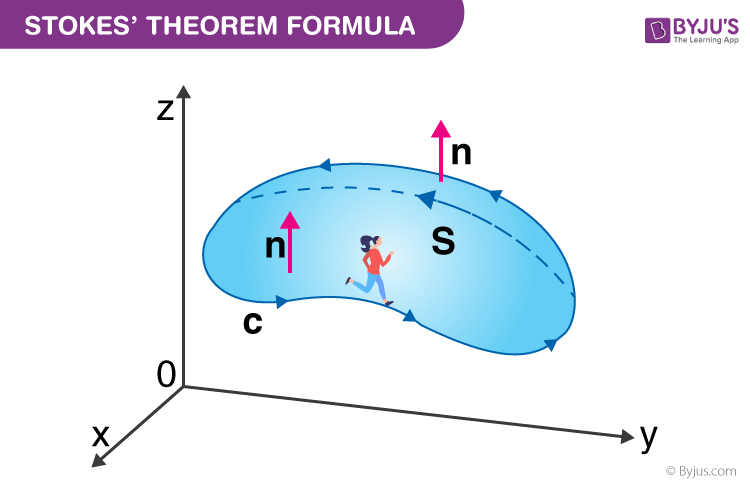
\includegraphics[width=0.8\textwidth]{./Stokes-Theorem-1.png} % Adjust the width as needed
\end{figure}
\section{Statistical Moments, Mean and Variance}
\subsection{Second Statistical Moment}
For some continuous random variable \(X\) with PDF \(f_X(x)\), the formula for the second statistical moment is 
\[
E(X^2) = \int_{-\infty}^{\infty} x^2 f_X(x) \, dx
\]
\subsubsection{Expanding the Second Statistical Moment to Relate to Mean and Variance}

We start with the integral definition of the second moment:
\[
E(X^2) = \int_{-\infty}^{\infty} x^2 f_X(x) \, dx
\]

Let \(\mu = E(X)\). We can express \(x^2\) in terms of \((x - \mu)\) as (simplify this equation below if  you don't believe me, the math works):
\[
x^2 = (x - \mu)^2 + 2\mu(x - \mu) + \mu^2
\]

Substituting this into the integral:
\[
E(X^2) = \int_{-\infty}^{\infty} \left[ (x - \mu)^2 + 2\mu(x - \mu) + \mu^2 \right] f_X(x) \, dx
\]

Splitting the integral into three terms:
\[
E(X^2) = \int_{-\infty}^{\infty} (x - \mu)^2 f_X(x) \, dx + 2\mu \int_{-\infty}^{\infty} (x - \mu) f_X(x) \, dx + \mu^2 \int_{-\infty}^{\infty} f_X(x) \, dx
\]

Evaluating each term:
\begin{enumerate}
\item \(\int_{-\infty}^{\infty} (x - \mu)^2 f_X(x) \, dx = \operatorname{Var}(X)\)
\item \(2\mu \int_{-\infty}^{\infty} (x - \mu) f_X(x) \, dx = 0\)
\item \(\mu^2 \int_{-\infty}^{\infty} f_X(x) \, dx = \mu^2\)
\end{enumerate}


So combining these, we have:
\[
E(X^2) = \operatorname{Var}(X) + \mu^2 = \operatorname{Var}(X) + [E(X)]^2
\]

\textbf{Footnote}: Why does the second integral go to zero? I don't believe you.\\
The second integral goes to zero because 
\[
2\mu \int_{-\infty}^{\infty} (x - \mu) f_X(x) \, dx = 2\mu \left(\int_{-\infty}^{\infty}x f_X(x)\, dx - \int_{-\infty}^{\infty} \mu f_X(x)\, dx \right)
\]

The first integral is the definition of the first statistical moment, so 
\[
\int_{-\infty}^{\infty}x f_X(x)\, dx = \mathbb{E}(X) = \mu
\]

For the second integral:
\[
\int_{-\infty}^{\infty} \mu f_X(x)\, dx = \mu \int_{-\infty}^{\infty} f_X(x)\, dx = \mu \cdot 1 = \mu
\]

So when you subtract these from each other, they cancel out.



\section{Differential Equations}
Standard equations relate one or more unknown functions (variables) to each other: 
\[y = 2x + 3\]
Differential equations relate one or more unknown functions and also their derivatives to each other:
\[\frac{dy}{dx} = 2x + 3\]

\textbf{What does a solution to a differential equation actually look like?}: A solution to a differential equation is a function (or a family of functions) that satisfies the differential equation when substituted into it. Unlike algebraic equations, where solutions are typically specific values of the variable(s) that make the equation true, solutions to differential equations are functions that describe how one variable changes with respect to another. For example, consider the ODE
\[\frac{dy}{dx} = y\] 
To solve this, we separate variables and integrate:

\[\frac{1}{y}dy = dx\]
\[\int \frac{1}{y}dy = \int dx\]
\[\ln |y| = x + C\]
\[y = Ce^x\]
Where C is some arbitrary constant. All functions of this family will have the relationship to their derivatives that is specified here:

\[y(x) = Ce^x\]
\[\frac{dy}{dx} = Ce^x = y(x)\]

\textbf{Note}: for PDE's the idea is generally the same, except it is a multivariable function that satisfies the partial differential equation (all partial derivatives match)

\subsection{Degree and Order}
\textbf{Order}: The order of a differential equation is the highest order of derivative that appears in the differential equation. For example,
\[\frac{dy}{dx} = 2x + 3\]
is first order, while
\[\frac{d^2y}{dx^2} = 2x + 3\]

is second order. \\

\textbf{Degree}: The degree of a differential equation is is the power to which the highest order derivative is raised after the equation has been retionalized to contain only integer powers of derivative. For example, the ODE	

\[\frac{d^3y}{dx^3} + x\left(\frac{dy}{dx}\right)^{\frac{3}{2}} + x^2y = 0\]
Is third order and second degree.\\
\subsection{Ordinary and Partial}
One sentence summary: look at the derivatives. If more than one variable is present in the denominator of the deriviatives (and you therefore have partial derivatives present) it is partial; otherwise the equation is ordinary. \\
\textbf{Ordinary} Ordinary Differential Equations (ODE's) have just a single independent variable and its derivatives in the equation. ODE's describe the relationship between a function and it's derivatives. 
\[\frac{dy}{dx} = y\] 
is ordinary. x is the independent variable because the function we're examining is y(x).

\textbf{Partial} Differential Equations (PDE's) have two or more independent variables. For example, if we have a function u(t,x) then this would be a PDE relating it to its derivatives:

\[\frac{\partial u}{\partial t} + c \frac{\partial u}{\partial x} = 0\]
\subsection{Separable ODE's}
A separable Differential Equation is one that can be written in the form:
\[\frac{dy}{dx} = g(x) \cdot h(y)\]

This is the definition because we can separate the dependent and independent variables on opposite sides of the equation:
\[h(y) \cdot dy = g(x) \cdot dx\]

\subsubsection{Solving Separable ODE's}
Solving Separable ODEs is extremely simple and can be done with the following steps:
\begin{enumerate}
\item Separate the variables
\item Integrate
\item Solve for \(y\) (dependent variable)
\end{enumerate}

\subsubsection{Example}
Consider the following separable ODE:
\[\frac{dy}{dx} = y \cdot \sin(x)\]

We will solve this using the steps outlined above:

\begin{enumerate}
\item \textbf{Separate the variables:}

\[ \frac{1}{y} \cdot dy = \sin(x) \cdot dx \]

\item \textbf{Integrate:}

Integrate both sides with respect to their respective variables:

\[ \int \frac{1}{y} \, dy = \int \sin(x) \, dx \]

This gives:

\[ \ln|y| = -\cos(x) + C \]

where \(C\) is the constant of integration.

\item \textbf{Solve for \(y\):}

To solve for \(y\), exponentiate both sides to remove the natural logarithm:

\[ y = e^{-\cos(x) + C} \]

We can rewrite \(e^C\) as a new constant, say \(C_1\):

\[ y = C_1 e^{-\cos(x)} \]

where \(C_1 = e^C\) is an arbitrary constant.
\end{enumerate}

Thus, the solution to the separable differential equation \(\frac{dy}{dx} = y \sin(x)\) is:

\[ y = C_1 e^{-\cos(x)} \]

where \(C_1\) is an arbitrary constant.
\subsubsection{Higher-Order ODEs and Separability}
Higher-order ODEs can technically be separable, but this is seldom the case in practice. Solving higher-order ODEs generally involves different techniques such as:
\begin{itemize}
\item Integration to reduce the order of the ODE.
\item Treating the higher-order ODE as a system of first-order ODEs.
\item Using special methods tailored to specific forms of higher-order ODEs.
\end{itemize}

For instance, a second-order ODE of the form:
\[\frac{d^2y}{dx^2} = f(x)\]
can be solved by integrating twice, which is a straightforward method but does not involve separation of variables in the same way as first-order separable ODEs.

\subsection{Exact ODE's}
An Exact ODE is an ODE that can be placed in the form

\[A(x,y) \, dx + B(x,y) \, dy = 0\]

where 
\[\frac{\partial A}{\partial y} = \frac{\partial B}{\partial x}\]

An exact ODE can be solved by following these steps:
\begin{enumerate}
\item Verify that the ODE is exact by checking if \(\frac{\partial A}{\partial y} = \frac{\partial B}{\partial x}\).
\item Find the potential function \(\psi(x, y)\) such that:
    \[ \frac{\partial \psi}{\partial x} = A(x, y) \]
    \[ \frac{\partial \psi}{\partial y} = B(x, y) \]

By integrating \(A(x, y)\) with respect to \(x\) to find the potential function \(\psi(x, y)\):
    \[ \psi(x, y) = \int A(x, y) \, dx + h(y) \]
\item Determine \(h(y)\) by differentiating \(\psi(x, y)\) with respect to \(y\), setting the result equal to \(B(x,y)\), and solving for \(h(y)\): 
    \[ \frac{\partial \psi}{\partial y} =  B(x, y) \]
\item Substitute \(h(y)\) back into \(\psi(x, y)\) to get the complete potential function and then this is the solution.
\end{enumerate}

\subsubsection{Example}
Consider the exact ODE:

\[ (2xy + 3) \, dx + (x^2 + 4y) \, dy = 0 \]

We will solve this using the steps outlined above:

\begin{enumerate}
\item \textbf{Verify Exactness:}
    \[ A(x, y) = 2xy + 3 \]
    \[ B(x, y) = x^2 + 4y \]
    Check if \(\frac{\partial A}{\partial y} = \frac{\partial B}{\partial x}\):
    \[ \frac{\partial A}{\partial y} = \frac{\partial}{\partial y} (2xy + 3) = 2x \]
    \[ \frac{\partial B}{\partial x} = \frac{\partial}{\partial x} (x^2 + 4y) = 2x \]
    Since \(\frac{\partial A}{\partial y} = \frac{\partial B}{\partial x}\), the equation is exact.

\item \textbf{Find the potential function \(\psi(x, y)\):}
    Integrate \(A(x, y)\) with respect to \(x\):
    \[ \psi(x, y) = \int (2xy + 3) \, dx = x^2y + 3x + h(y) \]

\item \textbf{Determine \(h(y)\):}
    Differentiate \(\psi(x, y)\) with respect to \(y\) and set it equal to \(B(x, y)\):
    \[ \frac{\partial \psi}{\partial y} = x^2 + h'(y) = x^2 + 4y \]
    This implies:
    \[ h'(y) = 4y \]
    Integrate to find \(h(y)\):
    \[ h(y) = 2y^2 + C \]

\item \textbf{Substitute back into potential function to obtain solution}:\\
    Substitute \(h(y)\) back into \(\psi(x, y)\):
    \[ \psi(x, y) = x^2y + 3x + 2y^2 + C \]

    The solution to the ODE is given by:
    \[ x^2y + 3x + 2y^2 = C \]
    where \(C\) is a constant.
\end{enumerate}

\subsection{Inexact ODE's}
Inexact ODE's are in the form

\[A(x,y) dx + B(x,y)dy = 0\]

But where
\[\frac{\partial A}{\partial y} \neq \frac{\partial B}{\partial x}\]
They can be made exact by multiplying by some integrating factor \(\mu(x,y)\) which will make the inexact equation exact:
\[\mu(x,y)A(x,y)dx + \mu(x,y)(B(x,y)dy = 0 \qquad \frac{\partial (\mu A)}{\partial y} = \frac{\partial( \mu B)}{\partial x}\]

Once the equation is exact, you can find its solution the same as described above. \\
\subsubsection{Finding Integrating Factor}
Recal that an integrating factor needs to satisfy 
\[\frac{\partial (\mu A)}{\partial y} = \frac{\partial( \mu B)}{\partial x}\]
If we assume \(\mu\) is a function of x (or y) alone, then the partial derivatives in this equation become just ordinary derivatives, and we can solve for \(\mu\) like this:

\[\frac{\partial (\mu A)}{\partial y} = \frac{\partial( \mu B)}{\partial x} \implies \mu \frac{\partial (A)}{\partial y} = \mu  \frac{\partial(B)}{\partial x} + B \frac{\partial( \mu)}{\partial x}\]

This is true because if you apply the product rule to both sides of the original equation iwth the assumption that \(\mu\) is only a function of x, you get

\[A \cdot \frac{\partial \mu}{\partial y} + \mu \frac{\partial (A)}{\partial y} = \mu  \frac{\partial(B)}{\partial x} + B \frac{\partial( \mu)}{\partial x}\]
And the first term \(\frac{\partial \mu}{\partial y} = 0\). So if \(\mu\) is only a function of y, the new equation can then be rearranged to get

\[\frac{\partial \mu}{\mu} = \frac{1}{B}\left( \frac{\partial A}{\partial y} - \frac{\partial B}{\partial x}\right)dx = f(x)dx\]
Where we can get \(\mu(x)\) from \(f(x)\) by solving the separable ODE 

 \[\frac{d \mu}{\mu} = f(x)dx\]

By integrating both sides and exponentiating, we get \(\mu\).
\subsubsection{Example}
Consider the following ODE:
\[ \frac{dy}{dx} = -\frac{2}{y} + \frac{3y}{2x} \]

Rearranging, we have:
\[ (4x + 3y^2) \, dx + 2xy \, dy = 0 \]

where
\[ A(x, y) = 4x + 3y^2 \]
\[ B(x, y) = 2xy \]

Computing the partial derivatives, we get:
\[ \frac{\partial A}{\partial y} = 6y \]
\[ \frac{\partial B}{\partial x} = 2y \]

Clearly, the ODE is not exact since \( \frac{\partial A}{\partial y} \neq \frac{\partial B}{\partial x} \).

However, we observe that:
\[ f(x) = \frac{1}{B} \left( \frac{\partial A}{\partial y} - \frac{\partial B}{\partial x} \right) = \frac{1}{2xy} (6y - 2y) = \frac{4}{2x} = \frac{2}{x} \]

This implies:
\[ \frac{d\mu}{\mu} = \frac{2}{x} \, dx \]

Integrating both sides, we get:
\[ \ln|\mu| = 2 \ln|x| + C \]
\[ \mu = e^C x^2 \]

Letting \( e^C = C_1 \), we have:
\[ \mu(x) = C_1 x^2 \]

Multiplying the original ODE by the integrating factor \( \mu(x) \):
\[ x^2 (4x + 3y^2) \, dx + x^2 (2xy) \, dy = 0 \]
\[ (4x^3 + 3x^2 y^2) \, dx + 2x^3 y \, dy = 0 \]

Checking for exactness again:
\[ \frac{\partial (4x^3 + 3x^2 y^2)}{\partial y} = 6x^2 y \]
\[ \frac{\partial (2x^3 y)}{\partial x} = 6x^2 y \]

Since \( \frac{\partial (4x^3 + 3x^2 y^2)}{\partial y} = \frac{\partial (2x^3 y)}{\partial x} \), the modified ODE is now exact.

To solve the exact ODE, find the potential function \( \psi(x, y) \):
\[ \frac{\partial \psi}{\partial x} = 4x^3 + 3x^2 y^2 \]

Integrating with respect to \( x \):
\[ \psi(x, y) = \int (4x^3 + 3x^2 y^2) \, dx = x^4 + x^3 y^2 + h(y) \]

Differentiate with respect to \( y \) and set it equal to the corresponding term in the original equation:
\[ \frac{\partial \psi}{\partial y} = 2x^3 y + h'(y) = 2x^3 y \]

Thus:
\[ h'(y) = 0 \]
\[ h(y) = C \]

Therefore, the potential function is:
\[ \psi(x, y) = x^4 + x^3 y^2 + C \]

The solution to the ODE is given by the level curves of \( \psi(x, y) \):
\[ x^4 + x^3 y^2 = C \]
\subsection{Clairaut's Equation}
Clairaut's equation is a special class of first order differential equatoin that can be written in the form:

\[y = x \frac{dy}{dx} + f\left(\frac{dy}{dx}\right)\]
Where \(f\) is a differentiable function that accepts the variable \(p  = \frac{dy}{dx}\). \\
By differentiating \(y = x p + f(p)\), we get

\[\frac{dy}{dx} = p + x \frac{dp}{dx} + f`(p)\frac{dp}{dx}\]
\[p = p + x \frac{dp}{dx} + f`(p)\frac{dp}{dx}\]
\[0=  x \frac{dp}{dx} + f`(p)\frac{dp}{dx}\]
\[0=  (x + f`(p))\frac{dp}{dx}\]

This is a system of equations. solving \(\frac{dp}{dx}=0\) gives the specific solution where p is a constant, and solving \((x + f`(p))=0\) gives the general solution.

\subsubsection{Example: Solving Clairaut's Equation}
Consider the Clairaut's equation:

\[ y = x \frac{dy}{dx} + \left(\frac{dy}{dx}\right)^2 \]

Let \( p = \frac{dy}{dx} \). Then the equation becomes:

\[ y = x p + p^2 \]

\begin{enumerate}
\item \textbf{Differentiate with Respect to \( x \)}

Differentiate both sides with respect to \( x \):

\[ \frac{dy}{dx} = p = p + x \frac{dp}{dx} + 2p \frac{dp}{dx} \]

\item \textbf{Simplify the Equation}

Subtract \( p \) from both sides:

\[ 0 = x \frac{dp}{dx} + 2p \frac{dp}{dx} \]

Factor out \( \frac{dp}{dx} \):

\[ 0 = (x + 2p) \frac{dp}{dx} \]

This implies two possible conditions:
\begin{enumerate}
\item \( \frac{dp}{dx} = 0 \)
\item \( x + 2p = 0 \)
\end{enumerate}

\item \textbf{Singular Solution}

If \( \frac{dp}{dx} = 0 \), then \( p \) is constant. Let \( p = c \), a constant. Substituting \( p = c \) into the original equation gives:

\[ y = x c + c^2 \]

This represents a family of straight lines parameterized by \( c \):

\[ y = c(x + c) \]

\item \textbf{General Solution}

For the general solution, solve \( x + 2p = 0 \):

\[ p = -\frac{x}{2} \]

Substitute \( p = -\frac{x}{2} \) back into the original equation:

\[ y = x \left(-\frac{x}{2}\right) + \left(-\frac{x}{2}\right)^2 \]
\[ y = -\frac{x^2}{2} + \frac{x^2}{4} \]
\[ y = -\frac{x^2}{4} \]

Therefore, the general solution is:

\[ y = -\frac{x^2}{4} \]

\end{enumerate}

\textbf{Combined Solution}

The combined solution consists of the family of straight lines and the parabolic curve:

\[ y = c(x + c) \]
\[ y = -\frac{x^2}{4} \]

where \( c \) is an arbitrary constant.

\subsection{Homogeneous ODEs}

A first-order differential equation is called homogeneous if it can be written in the form:
\[ \frac{dy}{dx} = f\left(\frac{y}{x}\right) \]
This means that the right-hand side is a function of the ratio \( \frac{y}{x} \) only. You can solve homogeneous ODEs via a substitution that makes them separable.

\begin{enumerate}
\item \textbf{Identify the Homogeneous Equation:}
   Start with an equation of the form \( \frac{dy}{dx} = f\left(\frac{y}{x}\right) \).

\item \textbf{Substitution:}
   Use the substitution \( v = \frac{y}{x} \). Consequently, \( y = vx \).
   Differentiate \( y = vx \) with respect to \( x \) to find \( \frac{dy}{dx} \):
   \[ \frac{dy}{dx} = v + x \frac{dv}{dx} \]

\item \textbf{Rewrite the Differential Equation:}
   Substitute \( y = vx \) and \( \frac{dy}{dx} = v + x \frac{dv}{dx} \) into the original equation. This transforms the original equation into an equation in terms of \( v \) and \( x \):
   \[ v + x \frac{dv}{dx} = f(v) \]
   Rearrange to isolate \( \frac{dv}{dx} \):
   \[ x \frac{dv}{dx} = f(v) - v \]
   \[ \frac{dv}{dx} = \frac{f(v) - v}{x} \]

\item \textbf{Separate Variables}
   Separate the variables \( v \) and \( x \):
   \[ \frac{dv}{f(v) - v} = \frac{dx}{x} \]

\item \textbf{Integrate Both Sides:}
   Integrate both sides with respect to their respective variables:
   \[ \int \frac{dv}{f(v) - v} = \int \frac{dx}{x} \]

\item \textbf{Solve the Integrals:}
   Find the antiderivatives of both sides:
   \[ \int \frac{dv}{f(v) - v} = \ln|x| + C \]
   Solve for \( v \):
   \[ G(v) = \ln|x| + C \]
   where \( G(v) \) represents the result of the integral on the left side.

\item \textbf{Substitute Back:}
   Replace \( v \) with \( \frac{y}{x} \):
   \[ G\left(\frac{y}{x}\right) = \ln|x| + C \]

\item \textbf{Solve for \( y \):}
   If possible, solve the equation for \( y \) in terms of \( x \).
\end{enumerate}
\subsection{Higher Degree First Order ODEs}
These are equations with \(p=\frac{dy}{dx}^n\) where \(n>1\). These are some methods of solving them:
\subsubsection{Equations Solvable for p}
Sometimes the LHS of the equation 
\[p^n + a_{n-1}(x,y)p^{n-1} + ... + a_1(x,y)p + a_0(x,y) = 0\]

can be directly factorized
\[(p - F1)(p - F2)...(P-Fn) = 0\]

you can then solve n first-degree first order ODEs and combine them into the general solution:
\[G_1(x,y)G_2(x,y)...G_n(x,y) = 0\]

\subsubsection{Equations Solvable for x or y}
\section{Objective Functions \& Loss Functions}

In machine learning and optimization, an \textbf{objective function} refers to the function that the algorithm aims to optimize, which can be either maximized or minimized depending on the problem. A \textbf{loss function} is a specific type of objective function that is always minimized and typically measures the discrepancy between predicted and actual values.

\subsection{Differences}
An objective function can represent both maximization and minimization problems, whereas a loss function is always minimized. In reinforcement learning, for instance, the objective is to maximize the expected cumulative reward, while in supervised learning, the goal is to minimize prediction errors.

\subsection{Common Examples}

\subsubsection{Objective Functions}
\begin{itemize}
    \item \textbf{Expected Cumulative Reward:} In reinforcement learning, the objective is to maximize the expected sum of discounted rewards:
    \[
    J(\theta) = \mathbb{E}_{\tau \sim \pi_{\theta}} \left[ \sum_{t=0}^{T} \gamma^t r_t \right]
    \]
    \item \textbf{Likelihood Maximization:} In probabilistic models, maximizing the likelihood of the observed data:
    \[
    J(\theta) = \sum_{i=1}^{N} \log p(y_i | x_i; \theta)
    \]
\end{itemize}

\subsubsection{Loss Functions}
\begin{itemize}
    \item \textbf{Categorical Cross-Entropy:} Used for classification tasks:
    \[
    L(\theta) = -\sum_{i=1}^{N} \sum_{c=1}^{C} y_{i,c} \log \hat{y}_{i,c}
    \]
    where \( y_{i,c} \) is the true label and \( \hat{y}_{i,c} \) is the predicted probability for class \( c \).
    
    \item \textbf{Mean Squared Error (MSE):} Common for regression tasks:
    \[
    L(\theta) = \frac{1}{N} \sum_{i=1}^{N} (y_i - \hat{y}_i)^2
    \]
\end{itemize}

\section{Linear Regression}
Linear regression is perhaps the simplest statistical learning algorithm. In Linear regression, assume we have an input data matrix \(X \in \mathbb{R}^{n \times d}\), where \(n\) is the number of training samples and \(d\) is the number of features.\\

Our objective is to learn weights \(w \in \mathbb{R}^d\)  and a bias term such that the prediction \(\hat{y} = Xw + b\) closely approximates \(y\).\\

We can wrap the bias term w into the weights by adding a column of 1's to \(X\) an augmented data matrix \(X' = [X, 1]\), where 1 is a column vector of 1's. Then \(w' = [w; b]\). (If this is confusing to you, don't think about it too hard. This is exactly equivalent to the original model and it doesn't change anything in its performance, it just simplifies the calculation of the gradient below because that way we dont' have to calculate two separate gradients.\\
\textbf{Note}: for Linear Regression to be an unbiased, efficient estimator the data must be \textbf{Homoscedatic}: meaing there is constant variance in the residuals:
\[\text{Var}(\epsilon_i) = \sigma^2 \forall i\]

where 
\[\epsilon_i = y_i - \hat{y}_i\]
and \( \hat{y}_i\) is our estimators prediction.
\subsection{Learning a Linear Regressor}
First we must define our loss function. For regression, MSE is a natural choice:
\[\mathcal{L}(w') = \frac{1}{n}(y - X'w')^2\]
Now let's calculate the gradient with respect to the \(w'\) (I'm just going to drop the prime to simplify the syntax. The bias term and column of 1's are still in w and X, respectively):\\

We start by expanding our loss function:
\[
\mathcal{L}(w) = \frac{1}{n} (y - Xw)^T (y - Xw)
\]
\[
\mathcal{L}(w)  = \frac{1}{n} \left( y^T y - y^T Xw - (Xw)^T y + (Xw)^T (Xw) \right)
\]
Notice that \( (Xw)^T y \) is a scalar and is equal to \( y^T Xw \). (It is scalar because \(X\) has shape \(n \times d\), wi is \(d \times 1\). so \((Xw)^T\) is \(1 \times n\). Then \(y\) is \(n\times 1\), so the product is \(1\times 1\). This is consistent with the fact that in linear regression we're "regressing" from \(n\) dimensions to 1. So our output \(y\) should be of shape \(n \times 1\) where we have \(n\) samples). Therefore:
\[
\mathcal{L} = \frac{1}{n} \left( y^T y - 2 y^T Xw + w^T X^T X w \right)
\]
Now we differentiate with respect to \(w\). The first term \( y^T y \) is constant so its derivative is 0.\\
The derivative with respect to \(w\) of \(- 2 y^T Xw\) is \(-2X^Ty\).\\
The derivative with respect to the third term \(w^T X^T X w\) is \(2X^TXw\) (because the derivative fo \(w^TAw\) where \(A\) is symmetric is \(2Aw\)).\\
So that gives us:
\[\nabla_w\mathcal{L} = \frac{1}{n}(-2X^Ty + 2X^TXw)\]
Which simplifies to
\[
\nabla_w\mathcal{L} = \frac{2}{n} X^T (Xw - y)
\]

\subsection{Learning with this gradient}
We do \textbf{not} use gradient descent to learn a linear regressor. We use maximum likelihood estimation. That means we set the gradient equal to 0 and solve for the \( w \) that minimizes the loss in a single step:

\[
-\frac{2}{n} X^T (y - X'w') = 0
\]
\[
X^T X' w' = X^T y
\]
\[
w' = (X^T X')^{-1} X^T y
\]
\section{Log-Derivative Trick}
The Log-Derivative Trick states that the derivative of the (natural) log of a function is related to the derivative of the function itself (because \( e \)). Let's say we have some multivariate function \( f_{\theta}(x) \) parameterized by \( \theta \):

\[
\nabla_{\theta} \log(f_{\theta}(x)) = \frac{\nabla_{\theta} f_{\theta}(x)}{f_{\theta}(x)}.
\]

So,

\[
f_{\theta}(x) \nabla_{\theta} \log(f_{\theta}(x)) = \nabla_{\theta} f_{\theta}(x).
\]

Note that \( f \) is a multivariate function parameterized by \( \theta \).

This is useful because differentiating the log of a function is often easier than differentiating the function itself. It's used all the time in anything involving Gaussian Distributions (see detection and estimation theory section). Let's say we have some Gaussian \( f(x; \mu, \sigma) \). The gradient of this with respect to \( \mu \) is:

\[
\nabla_{\mu} f(x; \mu, \sigma) = \frac{1}{\sqrt{2\pi\sigma^2}} e^{\left(-\frac{(x - \mu)^2}{2\sigma^2}\right)} \cdot \left(\frac{x - \mu}{\sigma^2}\right).
\]

But the log derivative is far easier to compute. We just take the derivative of the log of our function:

\[
\nabla_{\mu} \log f(x; \mu, \sigma) = \frac{x - \mu}{\sigma^2}.
\]
And then multiply it by the original function:
\[
\nabla_{\theta} f_{\theta}(x) = f_{\theta}(x) \cdot \nabla_{\mu} \log f(x; \mu, \sigma)
\]

Another thing that is useful (frankly, this is more useful than the above property): Because \(\log(x)\) is monotonically increasing, \(\nabla_{\theta}\log(f_{\theta}(x))\) will have the same extrema as \(\nabla_{\theta}f_{\theta}(x)\) for any function \(f\) that is strictly greater than 0. This means anywhere we're dealing with probability distributions, the log-derivative trick is extremely useful.
\section{Upper Confidence Bound}
Upper-confidence bound is a strategy for decision-making under uncertainty that seeks to balance exploration with exploitation to maximize the expected reward. It is frequently used in multi-armed bandit problems.\\

\textbf{Formula}:\\
Let's say that we have \(i\) possible arms (these could be actions, or state, action pairs) we could take at timestep \(t\), a hyperparameter \(c\) to control the tradeoff between exploration and exploitation, and a function \(N_i(t)\) that keeps track of the number of times we've visited \(i\). The UCB algorithm is this:

\[
i_t = \text{argmax}\left[\hat{\mu}_i + c\cdot \sqrt{\frac{\log t}{N_i(t)}} \right]
\]

It gives an upper bound on what the true reward is likely to be for arm \(i\) given the empirical reward \(\hat{\mu}_i\) and the number of visits \(N_i(t)\). The idea is that the more times an arm is pulled, the less uncertainty we have about what it's true utility is. The log term in the numerator also ensures that as t becomes large, the exploration term grows more slowly, naturally prioritizing exploitation as we reach the end of learning.\\
\textbf{Question}: at t=0, log t = 0. This doesn't make sense. We don't have no uncertainty at 0. \\
\textbf{Answer}: That's true. Typically UCB compensates for this by pulling each arm once at the start of the exploration process, or by making the numerator \(min(\log t, K)\) where K is the number of arms. 

\begin{figure}[H]
    \centering
    \includegraphics[width=0.8\textwidth]{./UCB\_heatmap.png} % Adjust the width as needed
\end{figure}
\section{Sobel Filtering}
Sobel Filters are an edge detection technique still very useful today, despite the presence of more sophisticated CV algorithms. It's especially useful as a data preprocessing step. It can efficiently and reliably detect edges by convolving the following filters with some image:

\[
G_x = \begin{bmatrix} -1 & 0 & +1 \\ -2 & 0 & +2 \\ -1 & 0 & +1 \end{bmatrix}, \quad 
G_y = \begin{bmatrix} +1 & +2 & +1 \\ 0 & 0 & 0 \\ -1 & -2 & -1 \end{bmatrix}
\]

\(G_x\) is for horizontal edge detection. \(G_y\) is for vertical edge detection. They get applied to some base image \(I\) like this: 

\[I_x = G_x \ast I\]
\[I_y = G_y \ast I\]

\(I_x\) shows horizontal edge intensity while \(I_y\) shows vertical edge intensity. We can then combine these two into a single gradient magnitude image, which captures the strength of the edge signal in in all directions:

\[|G| = \sqrt{I_x^2 + I_y^2}\]

Why in all directions, not just in vertical and horizontal directions? Becuase gradient edge strength in some arbitrary direction \(\theta\) = equals the square root sum of the strength in the horizontal and vertical directions. It's the same principle as in newtonian mechanics where a 2d vector force operating in any composite direction can be broken down with zero loss of information into its vertical and horizontal components. Pretty cool. 

\textbf{Sobel Filtering and Vector Calculus}: \\

The choice of the term 'edge strength gradient' to describe \(|G|\) is very deliberate. There is a deep relationship between Sobel filtering and vector calculus. First, imagine our image is a 2D scalar field where each pixel's intensity represents some function value \(I(x, y)\) at a coordinate pair \((x, y)\). The gradient of this discrete scalar field is:

\[
\nabla I = \left( \frac{\partial I}{\partial x}, \frac{\partial I}{\partial y} \right)
\]

Because this is a discrete scalar field, the gradients can be approximated using finite differences:

\[
\frac{\partial I}{\partial x} \approx I(x+1, y) - I(x-1, y), \quad \frac{\partial I}{\partial y} \approx I(x, y+1) - I(x, y-1)
\]

These values are closely approximated by the Sobel filters, which effectively compute the gradient by considering intensity changes across several pixels in a row or column, capturing an approximation of the literal edge gradient in the horizontal or vertical direction. Then, when we calculate

\[
|G| = \sqrt{I_x^2 + I_y^2}
\]

we are finding the gradient magnitude based on these two directional gradients. Thus, this filter identifies regions with rapid changes in gradient (edges) in arbitrary directions, capturing the strength of these transitions across the image.
\section{Kalman Filtering}
A Kalman filter is a recursive filter that uses a time-series of noisy measurements to produce estimates \(\hat{x}\) for a random variable \(x\) that tend to be less noisy than if a single estimate was taken. \\

A Kalman filter assumes that a random variable \(x_k\) at timestep \(k\) can have its state (position, velocity, acceleration, whatever) modeled with the following \emph{State Transition Equation}:

\[x_k = F_kx_{k-1} + B_ku_k + w_k\]

Where
\begin{itemize}
\item \textbf{\(X_k \in \mathbb{R}^n\)}: The state vector at time \(k\) encodes internal variables of the system.
\item \textbf{\(F_k \in \mathbb{R}^{n \times n}\)}: The state transition matrix, which describes how the state evolves over time in the absence of control inputs or noise. It encodes the dynamics of the system based on relationships between different components of the state.
\item \textbf{\(B_k \in \mathbb{R}^{n \times m}\)}: The control input matrix, which describes how external inputs affect the state. The control input vector \(u_k\) represents the actual external inputs applied to the system, while \(B_k\) parameterizes the relationship between them.
\item \textbf{\(w_k \sim \mathcal{N}(0, Q_k)\)}: Process noise. \textbf{Must be Gaussian}.
\end{itemize}
\subsection{Example Problem From Wikipedia}
Let's say we have a car moving alongside a frictionless track (so it only moves and accelerates in 1 direction. Let's also say that the car is blown along the track by the wind, which is a random variable that produces random accelerations. So the linear state space of the car at time \(k\) is given by 
\[
x_k = \begin{bmatrix}
x  \\
\dot{x}
\end{bmatrix}
\]

Where \(x\) gives the position and \(\dot{x}\) gives the velocity. The position and velocity are in turn parameterized by the following formulas:
\[x_k = x_{k-1} + \dot{x}_{k-1}\Delta t\]
\[\dot{x}_k = \dot{x}_{k-1}\]

(In the absence of external forces, velocity \(\dot{x}_k\) will remain constant and position \(x_k\) will change as a function of previous position and velocity.) So that means we have the following state transition matrix:

\[
F = \begin{bmatrix}
1 & \Delta t \\
0 & 1
\end{bmatrix}
\]

Because

\[
x_k = 
\begin{bmatrix}
x  \\
\dot{x}
\end{bmatrix}
=
\begin{bmatrix}
1 & \Delta t \\
0 & 1
\end{bmatrix}
\cdot
\begin{bmatrix}
x_{k-1} \\
\dot{x}_{k-1}
\end{bmatrix}
\]
But now we also need to account for the random accelerations:

\[
G = \begin{bmatrix}
\frac{1}{2}\Delta t^2  \\
\Delta t
\end{bmatrix}
\]

(this matrix gives the relationsihp acceleration has to position and velocity, respectively). So now we wind up with the final state transition equation, where \(a_k\) is an unknown input and G applies the effect of \(a_k\) to the state vector:

\[x_k = Fx_{k-1} + Ga_k\]

And now let's say \(a_k \sim N(0, Q)\), where \(Q\) gives the \emph{Noise Covariance Matrix}, which describes how the random variable \(a_k\) impacts each of the variables in our state transition equation. In real life, these things are determined empirically and depend on the physical characteristics of the vehicle, aerodynamics, friction, etc. In this toy problem, we're just setting them to be the following:

\[
Q = \begin{bmatrix}
\frac{\Delta t^4}{4} \sigma_a^2 & \frac{\Delta t^3}{2} \sigma_a^2 \\
\frac{\Delta t^3}{2} \sigma_a^2 & \Delta t^2 \sigma_a^2
\end{bmatrix}
\]

\textbf{Okay, so how do we predict the vehicle position with this?}:\\
A Kalman filter algorithm has two steps: prediction and correction:
\begin{itemize}
\item \textbf{Prediction Step}: We predcit: \[\hat{x}_k^- = F\hat{x}_{k-1}\]. Where \(\hat{x}_k^-\) gives the predicted state at \(k\) before the correction step. We also predcit the error covariance: \[P_k^- = FP_{k-1}F^T + Q\].
\item \textbf{Correction Step}: first we compute the Kalman Gain: \[K_k = P_k^-H^T(HP_k^-H^T + R)^{-1}\] The Kalman gain determines how much weight to give to the measurement vs. the prediction. \(H\) is the measurement matrix. In this example \(H = [1, 0]\) because we only directly observe the truck's position, not its velocity. \(R\) is the measurement noise. In this example it is: \(\mathbb{E}[v_kv_k^T]\). \\

After calculating the Kalman gain, we update our state estimate (we're essentially weighting it by how reliable we think the information is: \[\hat{x}_k = \hat{x}_k^- + K_k(z_k - H\hat{x}_k^-)\]. The matrix \((z_k - H\hat{x}_k^-)\) is called The Innovation, and measures the difference between the actual measurement and the predicted measurement. \\

Finally, we update the error covariance: \[P_k = (I - K_kH) P_k^-\]
\end{itemize}

And \(n\) gives the number of state variables and \(m\) gives the number of control variables.
\section{Kernel Density Estimation}

\subsection{What it is}
Kernel Density Estimation is a non-parametric statistical method used to estimate the probability density function (PDF) of a random variable. 

\subsection{How it works}
The general formula for KDE with a Gaussian kernel is given by:
\[
\hat{f}(x) = \frac{1}{nh} \sum_{i=1}^{n} \frac{1}{\sqrt{2\pi}} e^{-\frac{1}{2}\left(\frac{x - x_i}{h}\right)^2}
\]
where $\hat{f}(x)$ is the estimated density at point $x$.
\begin{itemize}
    \item $x_i$ are the $N$ data points for feature $i$. If we're doing classification, we can group features by class (so estimate PDF of feature $A$ for Class 1), or we can do for all classes in aggregate. It is also possible to do multivariate KDE, where we estimate the joint distribution for multiple features (features $A$ and $B$ for Class 1 or all Classes). It can also be done for regression (So 1 or more features when we're trying to do regression).
    \item $h$ is the bandwidth. The bandwidth is a positive scalar that dictates the width of the kernel function centered on each data point. Larger bandwidth = wider (more smoothed) distribution
\end{itemize}
Notice that we pass each observation in one at a time and then average across the distributions. This is because KDE assumes we have $N$ Gaussian distributions for each feature $C_i$, each of which is centered at the specific value for $A_{ij}$. We then average across all these distributions, and the result is an estimate of the real distribution for the data. (this is the same idea as Gaussian Mixture Models, though this is just a method for estimating PDF and GMMs are a full ML method used for inference).

\textbf{Steps}:\\
1.  we have a single point \(x\) we want to estimate the probability density of (we want \(p(x | x_n)\)), assuming that \(x\) is a part of the same probability distribution as our \(n\) samples \(x_n\).\\
2. we treat each sample \(x_i\) in \(x_n\) as if it were the center point of its own gaussian distribution, then we calculate the probability density for \(x\) coming from that distribution.\\
3. then we average across all these values and that gives us an approximation for \(p(x | x_n)\)\\
4. if we have \(k\) test samples \((x, y, ....)\), then we need to do this for each test point. \(O(kn)\) time. 

\textbf{Time Complexity and Fourier Domain}: 
\(O(nm)\) at inference, where \(n\) is the number of training samples in \(x_n\) and \(m\) gives the number of points we wish to estimate. If we do this in the fourier domain instead, we can do it in \(O(n) + O(m\log(m)\) time. We can write KDE in the fourier domain because
\[
\hat{f}(x) = \frac{1}{nh} \sum_{i=1}^{n} \frac{1}{\sqrt{2\pi}} e^{-\frac{1}{2}\left(\frac{x - x_i}{h}\right)^2} 
\]
Is equivalent to 
\[
\hat{f}(x) = \left(f_{empirical} * \frac{1}{h}K\left(\frac{.}{h}\right) \right)(x)
\]

KDE is really a convolution of our empircal observations \(x_n\) by the kernel function! this means we can take the Fast Fourier Transform of both the kernel function and the vector representing our n empircal datapoints, multiply them in the fourier domain, and then convert it back to the time domain. This is more efficient than doing it in the time domain. 
\subsection{When to use / When not to use}
\textbf{When to use:}
\begin{itemize}
    \item Gaussian KDE is particularly useful when you are dealing with continuous data and you want to avoid assuming a specific parametric form of the data distribution. It’s also useful when the goal is to get a smooth estimate of the data distribution.
    \item For data visualization and anomaly detection.
\end{itemize}

\textbf{When not to use:}
\begin{itemize}
    \item If your data is very high-dimensional, Gaussian KDE becomes less practical due to the curse of dimensionality—the amount of data needed to get a good estimate grows exponentially with the number of features.
    \item If your dataset is very large, KDE can be computationally expensive since it involves calculations over every pair of points.
\end{itemize}

\subsection{Pros / Cons}
\textbf{Pros:}
\begin{itemize}
    \item Non-parametric: Does not assume any underlying distribution for the data.
    \item Flexibility: Can model any shape of distribution (We don't have to choose a Gaussian Kernel)
	\item Smoothness: Can produce a smooth estimate of the density
\end{itemize}

\textbf{Cons:}
\begin{itemize}
    \item Computationally expensive with large datasets.
    \item Sensitive to the choice of bandwidth.
 	\item Performance degrades in higher dimensions (curse of dimensionality) The amount of data we need to get a decent distribution increases exponentially in the number of dimensions.
\end{itemize}
\subsection{Examples}

\subsubsection{Anomaly Detection in Network Security}
\begin{itemize}
    \item \textbf{Task:} Identifying unusual patterns or anomalies in network traffic to indicate security threats.
    \item \textbf{Use of KDE:} Apply KDE to model "normal" network traffic volume or request types, detecting anomalies as significant deviations.
\end{itemize}

\subsubsection{Customer Segmentation in Marketing}
\begin{itemize}
    \item \textbf{Task:} Segmenting customers based on purchasing behavior, demographics, or product interactions for targeted marketing.
    \item \textbf{Use of KDE:} Estimate the distribution of customer attributes (age, purchase frequency) to identify distinct segments for tailored marketing strategies.
\end{itemize}

% Include the figure
\begin{figure}[H]
    \centering
    \includegraphics[width=0.8\textwidth]{./gaussian_kde.png} % Adjust the width as needed
    \caption{Gaussian Kernel Density Estimation on a dataset. The figure shows the KDE curve with estimated densities at specific points. See gaussian kde plot.m for details}
    \label{fig:gaussian_kde}
\end{figure}
\section{Exponential Moving Average (EMA)} 
EMA is a technique in machine learning to reduce noise and ehnace generizability by updating two separate sets of parameters:
\begin{itemize}
\item \textbf{Params}: The normal model parameters that get updated directly after each batch via backpropagation and gradient descent
\item \textbf{Params\_ema}: A smoothed version of the parameters that are updated via exponential moving average. 
\end{itemize}
Again, EMA is useful for reducing noise, improving generalization, and stabilizing training. The update formula for EMA is:

\[\text{Params\_ema} = \alpha \cdot \text{Params\_ema} + (1 - \alpha) \cdot \text{Params}\]

Where \(\alpha\) is the decay rate (often set close to 1)

\section{Naive Bayes Classifiers}
Naive Bayes Classifiers are a probabilistic learning algorithm which uses Bayes Rule and the strong (naive) assumption that a set of features \(x_i \in X\) are each linearly independent of each other given the class label \(C_k\) to perform classification. 

\subsection{Mathematical Formulation and Theory}
Assume we have a set of class labels \(C_k \in C\) and a dataset where each sample represents a feature vector \(X\) of \(i\) features. We define the probability of each individual class given the observed data X as:

\[P(C_k | X)\]

We can use Bayes' Rule to expand like this:

 \[P(C_k | X) = \frac{P(C_k) \cdot P(X | C_k)}{P(X)}\]

The denominator is effectively constant because it does not vary across \(k\). The numerator is equivalent to the joint probability distribution:

\[P(C_k) \cdot P(X | C_k) = P(C_k, X)\]

Which in turn decomposes into this via the chain rule for repeated applications of conditional probability:
\[P(C_k, x_1, x_2, ... x_k) = P(x_1 | x_2, ... x_k, C_k) P(x_2 | x_3, ... x_k, C_k) ... P(x_k | C_k) P(C_k)\]

And then when we recall that all \(x_i\) are conditionally independent given \(C_k\) we get this:
\[P(C_k, x_1, x_2, ... x_k) = P(C_k) \prod_{i}P(x_i|C_k)\]

\textbf{Very Important Note}: For continuous features \(x_i\) Bayes' Rule and hence the above equality apply to probability \textit{density}, or likelihood, not the directy probability. Because of this, the value \(P(x_i|C_k)\) is nonzero and calculable as follows:

\[P(x_i = v|C_k) = \frac{1}{\sqrt{2\pi \sigma^2_k}}e^{\frac{(v - \mu_{k})^2}{2\sigma^2_k}}\]

Where \(\sigma^2_k\) gives the variance of feature \(x_i\) for all samples in class \(C_k\) and \(\mu_k\) is the mean of  feature \(x_i\) for all samples in class \(C_k\).

The decision rule for the classifier is this: 
\[\hat{y} = \text{argmax}_k \left(P(x_i = v|C_k) = \frac{1}{\sqrt{2\pi \sigma^2_k}}e^{\frac{(v - \mu_{k})^2}{2\sigma^2_k}}\right)\]

\subsection{Learning Process}
The learning process is extraordinarily simple. We estimate 

\[P(C_k) = \frac{\text{Num samples in class} C_k}{\text{Total Num samples}}\]
\[\mu_{ik} = \frac{1}{N_i} \sum_{j=1}^{N_i} x_{kj}\]
\[\sigma_{ik}^2 = \frac{1}{N_i - 1} \sum_{j=1}^{N_i} (x_{kj} - \mu_{ik})^2\]

Where \(N_i\) gives the number of samples for feature \(x_i\).



\begin{figure}[H]
    \centering
    \includegraphics[width=0.8\textwidth]{./setosa\_bayes.png} % Adjust the width as needed
\end{figure}
\section{Estimation Theory Fundamentals}
Estimation theory is a branch of statistics that deals with estimating the values of parameters based on measure empirical data that has a random component. In other words, if we have some signal \(x\) (a random variable), which is a normally distributed random variable:
\[
f(x | \mu_x, \sigma_x) = \frac{1}{\sigma_x \sqrt{2\pi}} e^{-\frac{(x - \mu_x)^2}{2\sigma_x^2}}
\]
Our goal in estimation theory is to estimate 
\[\hat{\mu}_x, \hat{\sigma}^2_x \approx \mu_x, \sigma_x^2\]
(Or whatever variables parameterize our distribution), given a set of observations and our underlying distribution. There are two primary approches to Estimation Theory, Classical and Bayesian. The classical approach includes Method of Moments (MoM, below) and Maximum Likelihood Estimation (MLE, further below).
\subsection{Method of Moments}
MoM is a common way to find our estimates \(\hat{\mu}_x, \hat{\sigma}^2_x\). In the method of moments, we set the \(k^{th}\) theoretical moment equal to the \(k^{th}\) practical moment and then solve for the parameter we're interested in estimating. \\\\
\(k^{th}\) theoretical moment:

\[m_k = \mathbb{E}[x^k] = \int_{-\infty}^{\infty}x^k f(x) dx\]
\(k^{th}\) practical moment: 
\[\hat{m}_k = \frac{1}{N}\sum_{i=0}^{N-1}x_i^k\]

\subsection{Method of Moments Example}
Let's say we have 

\[x = \{x_0, x_1,...,x_n\}\]

Where \(x\) are gathered from a Rayleigh Distribution:

\[f(x; \sigma^2) = \frac{x}{\sigma^2}e^{\frac{-x^2}{2\sigma^2}}\]

For a Rayleigh Distribution we know that our theoretical first and second moments are 

\[\mathbb{E}[x] = \sigma\frac{\pi}{2} \quad \mathbb{E}[x^2] = 2\sigma^2\]
 
We have to use the 2nd moment because if we do this for the 1st moment we will get \(\sigma\) in our equation, but no \(\sigma^2\), which is obviously the parameter we want to estimate (the variance). So our theoretical moment is 
\[\mathbb{E}[x^2] = 2\sigma^2\]

And our practical moment is 
\[\hat{m}_2 = \frac{1}{N}\sum_{i=0}^{N-1}x_i^2\]

So we solve like this:
\[\mathbb{E}[x^2] = \hat{m}_2\]

\[2\hat{\sigma}^2 = \frac{1}{N}\sum_{i=0}^{N-1}x_i^2\]

\[\hat{\sigma}^2 = \frac{1}{2N}\sum_{i=0}^{N-1}x_i^2\]

And we're done! This is our estimator. This is obviously a very simple example but it does reflect how method of moments works.
\subsection{Maximum Likelihood Estimation}
Let's say we have some random variable \(X\) whose pdf is \(f(X; A)\), which is parameterized by a constant unknown value \(A\). Let's imagine \(x\) is a sample we've made from the pdf above. At this point, \(x\) is a constant, so we have:

\[f(X=x; A) = g(A)\]

Since the function is now solely a function of \(A\), we can differentiate with respect to A to find the value of \(A\) that is most likely to have generated \(x\), which will correspond to the peak of the PDF. This is our maximum likelihood estimate. How do we solve this? We differentiate the log likelihood function with respect to \(A\) and set it equal to 0, then solve for \(A\):

\[\hat{A}_{MLE} = \frac{\partial \log(f(X=x; A) )}{\partial A} = 0\]

How does this work if we have multiple random variables parameterizing the distribution? I will show you. Let's assume we're given \(n\) i.i.d observations from a gaussian PDF

\[f(X; \mu, \sigma^2) =\frac{1}{\sqrt{2\pi\sigma^2}}e^{-\frac{(x-\mu)^2}{2\sigma^2}}\]
\[X = \{x_0, x_1,...,x_n\}\]

With unknown parameters \(\mu\) and \(\sigma\). First, we construct our likelihood function, which is the joint distribution across the individual densities associated with our \(n\) samples: 
\[L(\mu, \sigma^2; X) = \prod_{i=1}^n f(x_i; \mu, \sigma^2) = \prod_{i=1}^n \frac{1}{\sqrt{2\pi\sigma^2}}e^{-\frac{(x_i-\mu)^2}{2\sigma^2}}\]

\[L(\mu, \sigma^2; X) = \left(\frac{1}{\sqrt{2\pi\sigma^2}}\right)^n e^{\left( -\frac{1}{2\sigma^2}\sum_{i=1}^n (x_i-\mu)^2\right)}\]

Next we take the log of this:

\[
\log(L(\mu, \sigma^2; X)) = -\frac{n}{2}\log(2\pi\sigma^2) -\frac{1}{2\sigma^2}\sum_{i=1}^n (x_i-\mu)^2
\]

Then we differentiate with respect to each of the individual parameters we wish to find estimates for (it's that simple. just take the partial with repect to each and set equal to 0):

\[
\frac{\partial}{\partial \mu}\log(L(\mu, \sigma^2; X)) = \frac{\partial}{\partial \mu} \left( -\frac{1}{2\sigma^2}\sum_{i=1}^n (x_i-\mu)^2\right) = \frac{1}{\sigma^2}\sum_{i=1}^n (x_i-\mu) = 0
\]
(Note that the sigma goes away because we multiply each side by it after setting equal to 0)
\[
\frac{\partial}{\partial \sigma^2}\log(L(\mu, \sigma^2; X)) = \frac{\partial}{\partial \sigma^2}\left( -\frac{n}{2}\log(2\pi\sigma^2) -\frac{1}{2\sigma^2}\sum_{i=1}^n (x_i-\mu)^2 \right) = -\frac{n}{2\sigma^2} + \frac{1}{2(\sigma^2)^2}\sum_{i=1}^n(x_i-\mu)^2=0
\]
(Note that we're differentiating with respect to \(\sigma^2\) and not just \(\sigma\)). Then we solve for the parameter of interest in each equation:

\[\hat{\mu}=\frac{1}{n}\sum_{i=1}^nx_i\]

\[\hat{\sigma}^2 = \frac{1}{n}\sum_{i=1}^n (x_i-\hat{\mu})^2\]

And this gives us the \(\hat{\mu}\) and \(\hat{\sigma}^2\) that were most likely to have generated our observed data \(X\).
\subsection{Bayesian Estimation}
Now we explicitly model our parameter \(A\) as a random variable with a known distribution
\[A \sim f(A)\]

Where \(f(A)\) is called our Bayesian Prior. So we now have a random variable \(x\) whose PDF is parameterized by another random variable \(A\). We don't know what value \(A\) has taken on, so instead we seek to find an estimate \(\hat{A}\) that minimizes the Bayesian Minimum Mean Squared Error, which can be thought of as an error that captures the likelihood of observing both our data  \(x\) and our parameter \(A\), given the (unknown) underlying joint distribution of the random variables \(f(x,A)\):

\[Bmse = \int \int \left(A - \hat{A}\right)^2 f(x, A)dAdx\]

\[\hat{A} = \arg\min_A [Bmse]\]

As mentioned, we don't know \(f(x,A)\), so instead we have to solve for the joint distribution using Bayes' Rule. Because

\[f(A | x) = \frac{f(x,A)}{f(x)}\]

We can rewrite this as:

\[Bmse = \int \int \left(A - \hat{A}\right)^2 f(A | x)f(x)dAdx\]

Also, since the outer integral will evaluate to 1 always (x is drawn from a PDF), we can actually minimize the Bayesian MSE just by minimizing

\[\int \left(A - \hat{A}\right)^2 f(A | x)f(x)dA\]

To minimize this we take the derivative with respect to \(\hat{A}\) and set it equal to 0:
\[
\frac{\partial}{\partial \hat{A}} \int \left(A - \hat{A}\right)^2 f(A | x)f(x)dA = \int -2\left(A - \hat{A}\right) f(A | x)f(x)dA = 0 
\]

\[\int -2\hat{A} f(A | x)f(x)dA = \int -2A f(A | x)f(x)dA = 0\]

\[\hat{A} \int f(A | x)f(x)dA = \int A f(A | x)f(x)dA = 0\]

Because the integral on the left is just 1, we're left with 

\[\hat{A} = \int A f(A | x)dA \]

Which is our Minimum Mean Squared Error Estimator. Incidentally, it also equalls the conditional mean estimator \(\mathbb{E}[A|x]\), which makes sense. 
\subsection{Bayesian MMSE Example}
Suppose we have a pdf of a variable \(x\) parameterized by a random variable \(\theta\) (switching to a different variable name. Doesn't impact the math at all):

\[f(x|\theta) = \theta e ^{-\theta x}, x>0\]
Where our Bayesian Prior is:

\[f(\theta) = \lambda e^{-\lambda \theta}, \theta>0\]
We want to solve 

\[\hat{\theta} = \int \theta f(\theta | x)d\theta \]
To do this, we first need to solve 

\[f(x) = \int_0^{\infty} f(\theta, x) d\theta = \int_0^{\infty} \theta e^{-\theta x} \lambda e^{-\lambda \theta} d\theta = \frac{\lambda}{x+\lambda}\]
Now we plug all this into bayes rule:
\[f(\theta | x) = \frac{f(x|\theta) f(\theta)}{f(x)} = \frac{\theta e ^{-\theta x} \cdot  \lambda e^{-\lambda \theta}}{\frac{\lambda}{x+\lambda}}\]
Now we integrate:

\[\hat{\theta}_{MMSE} =  \int \theta f(\theta | x)d\theta =  \int \theta \cdot \left( \frac{\theta e ^{-\theta x} \cdot  \lambda e^{-\lambda \theta}}{\frac{\lambda}{x+\lambda}} \right) d\theta \]
Which eventually evaluates to:

\[\hat{\theta}_{MMSE}  = \frac{2}{x + \lambda}\]

\section{Detection Theory Fundamentals} 
Detection Theory refers to a set of statistical signal processing techniques that provide a means of differentiating between information-bearing patterns (alternate hypotheses) and random patterns (null hypotheses).
\subsection{Classical Detectors}
\subsubsection{Maximum Likelihood Detectors}
The maximum likelihood detector chooses the hypothesis with the greatest probability of being true:

\[
\text{Choose } H_1: \log \left(\frac{f(x; H_1)}{f(x; H_0)}\right) > 0
\]
\[
\text{Choose } H_0: \log \left(\frac{f(x; H_1)}{f(x; H_0)}\right) < 0
\]

\subsubsection{Neyman-Pearson Detectors}

The Neyman Pearson Detector also works by forming a log likelihood ratio, but instead of merely choosing the most likely hypothesis, we instead calculate a desired probability of false alarm for our system and tune our system to have said \(P_{FA}\) with the introduction of a variable \(\gamma\) (gamma):


\[
\text{Choose } H_1: \log \left(\frac{f(x; H_1)}{f(x; H_0)}\right) > \log(\gamma)
\]
\[
\text{Choose } H_0: \log \left(\frac{f(x; H_1)}{f(x; H_0)}\right) < \log(\gamma)
\]

Both Maximum Likelihood Detectors and Neyman-Pearson Detectors rely on the same problem-solving flow; the only difference between them (specified above) is the thresholding value choice.

\subsubsection{Binary Detection example with N observations}
We have \(N\) observations of some iid random variable and we wish to decide whether it belongs to distribution \(f_0(x; 0, \sigma^2)\) or distribution \(f_1(x; A, \sigma^2)\). \\

We begin by forming two PDFs representing the joint PDF of the observed data x parametrized by each of the two distributions:

\[f_0(x; 0, \sigma^2)  = \prod_{i=1}^N \frac{1}{\sqrt{2\pi \sigma^2}}e^{-\frac{x_i^2}{2\sigma^2}}\]

\[f_1(x; A, \sigma^2)  = \prod_{i=1}^N \frac{1}{\sqrt{2\pi \sigma^2}}e^{-\frac{(x_i - A)^2}{2\sigma^2}}\]

Then we form the log likelihood ratio and set equal to 0:
\[\Lambda(x) = \log \left( \frac{f_1(x; A, \sigma^2)}{f_0(x; 0, \sigma^2)}\right)\]

Which gives us: 

\[
\sum_{i=1}^N-\frac{(x_i - A)^2}{2\sigma^2} + \frac{x_i^2}{2\sigma^2} \mathrel{\substack{H_1 \\ \gtrless \\ H_0}} 0
\]
This will simplify to 

\[
\sum_{i=1}^N x_i- \frac{A}{2} \mathrel{\substack{H_1 \\ \gtrless \\ H_0}} 0
\]
Now is where our two methods diverge. I'll start with Maximum Likelihood detection. In maximimum likelihood detection \(\gamma\) is set to 1 because \(\log(1) = 0\). We can calculate the \(P_D\) and \(P_{FA}\) for our detector using the Q function, which is the tail distribution function of the standard normal distribution (1 - CDF): 
\[Q(z) = \frac{1}{\sqrt{2\pi}}\int_z^\infty e^{-\frac{u^2}{2}}du\]

We can use these formulas to calculate  \(P_D\) and \(P_{FA}\) for our problem:

\[z_0 = \frac{\gamma - \mu_0}{\frac{\sigma_0}{\sqrt{N}}} \quad P_{FA} = Q(z_0)\]
\[z_1 = \frac{\gamma - \mu_1}{\frac{\sigma_1}{\sqrt{N}}} \quad P_{D} = Q(z_1)\]

So for our problem:

\[z_0 = \frac{1 - 0}{\frac{\sigma}{\sqrt{N}}} \quad z_1 = \frac{1 - A}{\frac{\sigma}{\sqrt{N}}}\]
And then \(P_{FA} = Q(z_0), \quad P_D = Q(z_1)\).

If we let \(A=1, N=1\), then \(P_D  = Q(0) = 0.5, \quad P_{FA} = Q(1) = 0.15\)\\

In Neyman-Pearson Detection, we choose \(\gamma\) based off our desired \(P_{FA}\):

\[\gamma = Q^{-1}(P_{FA})\]


We then have to unnormalize because the Q function is for a standard normal distribution, and have also to remember that since we have \(N\) samples, our variance is scaled down by the number of observations:

\[\gamma_{\text{final}} = \gamma \frac{\sigma_0}{\sqrt{N}} + \mu_0 = \gamma \frac{\sigma}{\sqrt{N}}+ 0\]

This is then fed into our Q function to get the probability of detection (remember that we already know the \(P_{FA}\)):

\[P_D = Q\left(\frac{\gamma_{\text{final}}}{\frac{\sigma^2}{\sqrt{N}}} \right)\]
\subsection{Bayesian Detectors}
In the above detection methods, each hypothesis is implicitly considered to  be equally likely. If this is not the case and we know the probabilities of our hypotheses, we can incorporate this into our detectors. This is called Bayesian Detection. \\

The general bayesian detector aims to minimize the risk. The Risk \(\mathcal{R}\) sum of the probabilities of each particular error weighted by an error-specific cost penalty (this is for a binary detector, but generalizes easily to multiple hypotheses):

\[\mathcal{R} = C_{01}P(H_0 | H_1)P(H_1) + C_{10}P(H_1 | H_0)P(H_0)\]

We choose the detector that minimizes risk.\\

It actually turns out that this detector is strikingly similar to the likelihood ratio formed above in classical detection. The formula for \(\gamma\) is this:

\[\gamma = \frac{(C_{10} - C_{11})P(H_0)}{(C_{01} - C{11})P(H_1)}\]

We then plug this into our formulas for \(z_0\) and \(z_1\) the same as above to compute the probabilities of false alarm and detection for our detector.


\[z_0 = \frac{\gamma - \mu_0}{\frac{\sigma_0}{\sqrt{N}}} \quad P_{FA} = Q(z_0)\]
\[z_1 = \frac{\gamma - \mu_1}{\frac{\sigma_1}{\sqrt{N}}} \quad P_{D} = Q(z_1)\]

In general, Bayesian detectors are challenging because we need to set costs, which means we probably have to compute the false alarm probability to determine what cost is required. So you basically have to implement a neyman-pearson detector and then pose it as a bayesian detector (this is true because to compute the false alarm probability you're basically implementing a classical detector already). But bayesian detectors do have their place.

\section{Bhattacharyya Distance}

\subsection{What it is}
The Bhattacharyya distance is a measure of divergence between two probability distributions, providing a quantitative measure of their similarity.

\subsection{How it works}
For discrete probability distributions \(P\) and \(Q\) with PDFs \(p(x)\) and \(q(x)\), the Bhattacharyya distance \(D_B\) is defined as:
\[ D_B(P, Q) = -\ln\left(\sum_{x \in X} \sqrt{p(x)q(x)}\right) \] 

For continuous probability distributions it is:
\[
D_B(P, Q) = -\ln\left(\int_{X} \sqrt{p(x)q(x)} \, dx\right)
\]
The core of the Bhattacharyya distance lies in the term \(\sqrt{p(x)q(x)}\), which computes the geometric mean of the probabilities \(p(x)\) and \(q(x)\) for each outcome \(x\). The sum or integral of these geometric means over all possible outcomes \(x\) yields a measure of the overlap between the two distributions. The more similar the distributions are, the larger the sum (or integral) of the geometric means will be because \(a^2 \geq a \times b\) \(\forall\) \(a, b \in [0, 1]\) \(st.\) \(a \geq b, a + b = 1\). Conversely, distributions with less overlap will result in a larger Bhattacharyya distance.

\subsection{When to use / When not to use}
\textbf{When to Use:}
\begin{itemize}
    \item To compare the similarity between two distributions in classification, clustering, or anomaly detection tasks.
	\item \textbf{Specifically, to compare the amount of overlap between probability distributions.} The overhap (think, area under the curve of both integrals) is literally just the integral product of these two PDF's over X. This is the exact formula for Bhattacharyya Distance (we add the square root because it makes small numbers associated with PDFs more stable. \(\sqrt{0.01 \times 0.99}\) is ten times greater than \(0.01 \times 0.99\) ). So this is a more balanced representation of the region of overlap (the values are larger because \(\sqrt{a \times b} \geq a \times b\) \( \forall a,b \in [0,1]\))
\end{itemize}
\textbf{When Not to Use:}
\begin{itemize}
    \item For tasks that require a direct interpretation of information gain or loss between distributions, where measures like Kullback-Leibler divergence might be more appropriate.
    \item In high-dimensional spaces without appropriate dimensionality reduction, as the measure may become less informative.
\end{itemize}

\subsection{Pros / Cons}
\textbf{Pros:}
\begin{itemize}
    \item It is symmetric, meaning 
\[ D_B(P, Q) = D_B(Q, P) \]
Unlike KL divergence, which directly quantifies the information gain when one distribution is used to approximate another (thus being inherently asymmetric).

    \item Applicable to both discrete and continuous distributions, offering broad utility.
\end{itemize}
\textbf{Cons:}
\begin{itemize}
    \item May not capture complex differences in distribution shapes, especially in high-dimensional spaces.
\end{itemize}
\section{Bias-Variance Tradeoff}
The bias variance tradeoff is a fundamental concept in machine learning which relates two different forms of error that can impact the generalization ability of a model: bias (underfitting) and variance (overfitting). It states that as model complexity increases, the bias of the model will decrease while the variance increases.

\subsection{Mathematical Formulation of Bias-Variance Tradeoff for MSE}
First, we define the MSE as follows:

\[\mathbb{E}[(f(x) - \hat{f}(x))^2]\]

Where \(\hat{f}(x)\) gives our prediction for some input \(x\) and \(f(x)\) gives the true underlying function that represents the ideal relationship between the input \(x\) and the output. Now, we add and subtract the expectation of the prediction of our model inside the equation:


\[\mathbb{E}[(f(x) - \mathbb{E}[\hat{f}(x)] + \mathbb{E}[\hat{f}(x)] - \hat{f}(x))^2]\]

This expression is equal to the one above, but we can expand it differently: 

\[
\mathbb{E}[(f(x) - \mathbb{E}[\hat{f}(x)] + \mathbb{E}[\hat{f}(x)] - \hat{f}(x))^2] = 
\]
\[
\mathbb{E}\left[ (f(x) - \mathbb{E}[\hat{f}(x)])^2 +  2((f(x) - \mathbb{E}[\hat{f}(x)]) \cdot(\mathbb{E}[\hat{f}(x)] - \hat{f}(x))) + ( \mathbb{E}[\hat{f}(x)] - \hat{f}(x))^2\right]
\]

We can distribute the expectation across these three terms:

\[
\mathbb{E}\left[(f(x) - \mathbb{E}[\hat{f}(x)])^2\right] + \mathbb{E}\left[2((f(x) - \mathbb{E}[\hat{f}(x)]) \cdot(\mathbb{E}[\hat{f}(x)] - \hat{f}(x)))\right] + \mathbb{E}\left[( \mathbb{E}[\hat{f}(x)] - \hat{f}(x))^2\right]
\]

The first term is actually constant because \(f(x)\), being ideal, is not stochastic; and \(\mathbb{E}[\mathbb{E}[x]] = \mathbb{E}[x] \quad \forall x\) (as long as x is integrable and the expectations are taken over the same probability space), so we can drop the expectation:

\[\mathbb{E}\left[(f(x) - \mathbb{E}[\hat{f}(x)])^2\right] = (f(x) - \mathbb{E}[\hat{f}(x)])^2\]
The second term goes to zero because 

\[
\mathbb{E}[\mathbb{E}[\hat{f}(x)]] - \mathbb{E}[\hat{f}(x)] = 0
\]

so 

\[
\mathbb{E}\left[2((f(x) - \mathbb{E}[\hat{f}(x)]) \cdot (\mathbb{E}[\hat{f}(x)] - \hat{f}(x)))\right] = 0
\]

The third term is the formula for the variance of \(\hat{f}(x)\):

\[
\mathbb{E}\left[( \mathbb{E}[\hat{f}(x)] - \hat{f}(x))^2\right] = \text{Var}(\hat{f}(x))
\]

The first term corresponds to the bias squared. The second term is the variance. Then we add in an irreducible noise term \(\sigma^2\), which comes from flaws in the dataset used to train \(\hat{f}(x)\). So, taken together, we have:

\[
\mathbb{E}[(f(x) - \hat{f}(x))^2] = (f(x) - \mathbb{E}[\hat{f}(x)])^2 + \mathbb{E}\left[( \mathbb{E}[\hat{f}(x)] - \hat{f}(x))^2\right]  + \sigma^2 
\]

This means that any model \(\hat{f}(x)\) trained via MSE can have its error broken down into these three components. Other error functions have different, but similar derivations. Most commonly used error functions are separable into these three components, but there may be some which are not. nevertheless, this concept holds in general for pretty much all machine learning models.

\subsection{Why is it a tradeoff?}
Why can't you lower both bias and variance all the way to zero? Why does increasing model complexity to lower bias necessarily mean we increase variance? 

\subsubsection{Why Bias Decreases as Model Complexity Increases}

Imagine we have an \(m\) degree polynomial and we wish to approximate it with a \(k\) degree Ordinary Least Squares Estimator. This is literally just a line of best fit \(\hat{f}(x)\) estimating the curve of some higher dimensional line \(f(x)\):

\[\hat{f}(x) = \sum_{j=0}^k \hat{\beta}_jx^j\]

Where \(\hat{\beta}_j\) gives the jth coefficient, and \(x^j\) is just some input \(x\) raised to the jth power. (\(x, x^2, x^3, ...\)). The bias for this function will be 

\[\left(\mathbb{E}[\hat{f}(x)] - f(x)\right)^2 = \left(\mathbb{E}\left[\sum_{j=0}^k\hat{\beta}_j x^j\right] - \sum_{j=0}^m  \beta_j^*x^j\right)^2\]

Because \(\mathbb{E}[\hat{\beta}_j] = \beta_j^*\) we have for \(k < m\):
\[\left(\mathbb{E}[\hat{f}(x)] - f(x)\right)^2  = \left(\sum_{j=0}^k  \beta_j^*x^j - \sum_{j=0}^m  \beta_j^*x^j\right)^2 = \left(- \sum_{j=k+1}^m  \beta_j^*x^j\right)^2\]

This term wil obviously get decrease as k approaches m because the number of terms being summed over will shrink. for \(k \geq m\) the theoretical bias is 0 because \(\mathbb{E}[\hat{\beta}_j ] = \beta_j^*\), and \(\beta_j^* = 0 \quad \forall j >=m\). So while obviously the practical bias may not go to 0, we observe that the bias is directly proportional to \((m - k)\) and when \(k > m\) the theoretical bias goes to 0. Thus, as model complexity incresases,  bias decreases. \\
\subsubsection{Why Variance Increases as Model Complexity Increases}

Consider again our least squares estimator:

\[\hat{f}(x) = \sum_{j=0}^k \hat{\beta}_j x^j\]

The variance of  this estimator's output is: 
\[
Var\left(\sum_{j=0}^k \hat{\beta}_j x^j\right) = \mathbb{E}\left[\left(\sum_{j=0}^k \hat{\beta}_j x^j\right)^2- \left(\mathbb{E}\left[\sum_{j=0}^k \hat{\beta}_j x^j\right]\right)^2\right] 
\]
\textbf{If we expand the first term we get} (note that becasue the sum of the variances is the variance of the sums, I am taking the liberty of distributing the expectation):

\[
\mathbb{E}\left[\left(\sum_{j=0}^k \hat{\beta}_j x^j\right)^2\right] = \mathbb{E}\left[\sum_{j=0}^k \sum_{l=0}^k \hat{\beta}_j \hat{\beta}_l x^j x^l\right] = \sum_{j=0}^k \sum_{l=0}^k \mathbb{E}\left[\hat{\beta}_j \hat{\beta}_l\right] x^j x^l
\]
\textbf{Now, expanding the second term, we get}:

\[
\left( \mathbb{E} \left[ \sum_{j=0}^{k} \hat{\beta}_j x^j \right] \right)^2 
= \left( \sum_{j=0}^{k} \mathbb{E} \left[ \hat{\beta}_j \right] x^j \right)^2
= \sum_{j=0}^{k} \sum_{l=0}^{k} \mathbb{E} \left[ \hat{\beta}_j \right] \mathbb{E} \left[ \hat{\beta}_l \right] x^j x^l
\]
Note that the definition of covariance can be used to combine these two equations together:

\[Var\left(\sum_{j=0}^k \hat{\beta}_j x^j\right) = \sum_{j=0}^k \sum_{l=0}^k \mathbb{E}\left[\hat{\beta}_j \hat{\beta}_l\right] x^j x^l -  \sum_{j=0}^{k} \sum_{l=0}^{k} \mathbb{E} \left[ \hat{\beta}_j \right] \mathbb{E} \left[ \hat{\beta}_l \right] x^j x^l\]

\[Var\left(\sum_{j=0}^k \hat{\beta}_j x^j\right) = \sum_{j=0}^k \sum_{l=0}^k \left(\mathbb{E}\left[\hat{\beta}_j \hat{\beta}_l\right] - \mathbb{E} \left[ \hat{\beta}_j \right] \mathbb{E} \left[ \hat{\beta}_l \right]\right)x^j x^l\]

The definition of covariance is 
\[
Cov(\hat{\beta}_j, \hat{\beta}_l) = \mathbb{E}[\hat{\beta}_j \hat{\beta}_l] - \mathbb{E}[\hat{\beta}_j] \mathbb{E}[\hat{\beta}_l]
\]

Note that we have a large exponential value for \(x\) out front in this equation and not in the previous ones because we're multiplying the \(x\) input values with each other inside the summation farther above.
So we can write the variance in terms of the covariance between our \(k\) coefficients like this:
\[Var\left(\sum_{j=0}^k \hat{\beta}_j x^j\right) =  \sum_{j=0}^k \sum_{l=0}^k Cov(\hat{\beta_j}, \hat{\beta_l})x^j x^l\]

Now consider what happens when we add an additional \((k+1)^{th}\) parameter. When we add a new parameter, our estimator becomes:

\[\hat{f}_{k+1}(x) = \hat{f}_k(x) + \beta_{k+1}x^{k+1}\]

And the variance becomes:

\[Var[\hat{f}_{k+1}(x)] = Var[\hat{f}_{k}(x)] + (x^{k+1})^2Var(\hat{\beta}_{k+1}) + 2x^{k+1}\sum_{j=0}^k x^j Cov(\hat{\beta})j, \hat{\beta}_{k+1})\]

This is the original term, plus the variance of the Which is clearly going to be greater than the original variance. Therefore the variance of the model's output increases as model complexity increases. \\

\textbf{Note}: I have chosen a ML model where the variance of that model's output is directly expressible in terms of the number and values of the weights for that model. This is, in fact, the case for all ML models, even things as complicated as transformers (the output of a transformer is still a function of its inputs, so you can just compute the variance of that output -- in theory, it would be way to complex to compute in practice). so this tradeoff, while I've proven it for the simplest possible machine learning model, holds across all machine learning architectures and problem types. It's never going away. this is a fundamental result. 

\textbf{Note}: This also helps to explain power laws for neural scaling, which state that the amount of data needed to train a model is proportional to the number of parameters in that model (if you need 1,000 samples to train a model with 8 parameters, you need 10,000 samples to train a model with 80 parameters). It explains it (or at least acts as a mathematical foundation for understanding it) because the bias and variance are proportional (in some way, depending on the model, and not necessarily the same way for the two) to the number of paramters. 


 \section{KL-Divergence}
\subsection{What it is}

The Kullback–Leibler divergence (or information divergence, information gain, or relative entropy) is a way of comparing two probability distributions: a "true" probability distribution \(p(X)\), and an arbitrary probability distribution \(q(X)\). Although it is sometimes used as a 'distance metric,' KL divergence is not a true metric since it is not symmetric and does not satisfy the triangle inequality (making it a semi-quasimetric).


\subsection{How it works}
Imagine we have two distributions: a "true" probability distribution \(p(X)\), and an arbitrary probability distribution \(q(X)\). If we compress data in a manner that assumes \(q(X)\) is the distribution underlying some data, when, in reality, \(p(X)\) is the correct distribution, the Kullback–Leibler divergence is the number of average additional bits per datum necessary for compression (the nuts and bolts of this are deep into Information Theory, just trust that it works). It is defined


\[
\begin{aligned}
D_{KL}(p(X)||q(X)) &= -\sum_{x \in X} p(x) \log q(x) - \left(-\sum_{x \in X} p(x) \log p(x)\right) &= \sum_{x \in X} p(x) \log\left(\frac{p(x)}{q(x)}\right)
\end{aligned}
\]


\subsubsection{Detection Theory Intuition on KL-Divergence}

Note that KL-Divergence is literally just the expectation of the log likelihood ratio:
\[
\begin{aligned}
D_{KL}(p(X)||q(X)) &= \sum_{x \in X} p(x) \log\left(\frac{p(x)}{q(x)}\right) &= \mathbb{E}\left[\log\left(\frac{p(x)}{q(x)}\right)\right]
\end{aligned}
\]

In detection theory, we use the log likelihood ratio test to decide between two hypotheses:


\begin{itemize}
    \item \(H_0\): The data is generated null distribution \(q(x)\) (eg: N(2,1)).
    \item \(H_1\): The data is generated some other distribution \(p(x)\) (eg: N(3,1).
\end{itemize}

The log-likelihood ratio for an observed sample \(x\) is given by:

\[ \Lambda(x) = \log\left(\frac{p(x)}{q(x)}\right) \]

This ratio tells us how much more likely it is that the observed sample came from distribution \(p(x)\) rather than \(q(x)\). If the value of \(\Lambda(x)\) is high, we define some minimum threshold the LLR must exceed to conclude the data comes from \(p(x)\). Otherwise we conclude the data came from \(q(x)\). Another way of looking at this is that if the LLR exceeds our threshold we conclude \(p(x)\) and \(q(x)\) are different distributions; otherwise we cannot conclude that. The key insight here which should help with your intuition is that the higher the LLR is, the more likely it is p(x) and q(x) are different distributions. So the greater the KL-divergence is, the more different the distributions are. 

\subsection{When to use / Pros}
\begin{itemize}
    \item To compare the output distribution of a model to the true data distribution, especially in generative models or for model calibration.
    \item  \textbf{Information Theory Context} In Bayesian frameworks to quantify the information gain after updating models with new data.
	\item \textbf{Gradient Based optimization} In machine learning, especially with neural networks, KL divergence has a nice gradient that can be used in backpropagation, which is not the case with all metrics
	\item Great for anything related to comparing probability distributions, especially from a Bayesian perspective.
	\item Useful for evaluating the impact of model updates or changes in model complexity.
\end{itemize}

\subsection{When not to use / Cons}
\begin{itemize}
    \item Don't use when distributions don't overlap (it is undefined then)
    \item When a symmetric distance metric that obeys the triangle inequality is required, such as in clustering or multidimensional scaling.
	\item \textbf{Comparing Distributions for Overlap} Bhattacharyya distance is better if you're specifically interested in the overlap between two distributions (as opposed to just measuring their similarity), as that is what it is designed to measure
	\item \textbf{Robustness to Sample Variability:} When working wiht empirical data where sample variability may affect the distributions, metrics that are less sensitive to outliers or the lack of data points in regions of the space (like the Wasserstein distance) might be more appropriate.
	\item \textbf{Clustering and Multidimensional Scaling:} It should not be used in clustering algorithms that require a metric space (like k-means or hierarchical clustering) or in multidimensional scaling which requires distances that obey the triangle inequality.
\end{itemize}

\subsection{Examples}
\subsubsection{Model Selection in Statistical Learning}
\begin{itemize}
    \item \textbf{Task:} Choosing the best probabilistic model from a set of candidate models that best describes an observed set of data.
    \item \textbf{Use of KL Divergence:} Employ KL divergence to compare the estimated probability distribution of each model against the empirical distribution of the data, selecting the model with the lowest KL divergence.
\end{itemize}
\subsubsection{Use in Variational Autoencoders (VAEs)}
\begin{itemize}
    \item \textbf{Task:} To learn a generative model that can produce data similar to the input data by encoding the inputs into a latent space and then decoding from this space.
    \item \textbf{Use of KL Divergence:} In VAEs, KL divergence is used to regularize the encoder by measuring the difference between the distribution of the encoded latent variables (the tensors being passed through the bottleneck layer) and a prior distribution (often a Gaussian). This encourages the latent space to adhere to a known distribution, which improves the generality and interpretability of the model. It is not directly used to compare the output of the VAE to the ground truth data distribution; rather, it's used to ensure the latent space representation is regularized, while reconstruction loss (like MSE) measures the difference between the output and the ground truth.
\end{itemize}

\section {Radial Basis Function Networks}
Radial Basis Function Networks (RBFs) are a kind of neural net that use radial basis functoins as their activation function. The output of the network is a linear combination of radial basis functoins of the inputs and neuron parameters. RBFs are unique in that they are universal function approximators, unlike other relatively simple ML models like GMMs and KNNs. 

\subsection{What is a radial basis function?}
A radial basis function is a real-valued function \(\rho\) whose value depends only on the distance between the input and some fixed point, either the origin (so that \(\rho(x) = \hat{\rho}(||x||)\)) or some fixed point \(c\) called the center (so that \(\rho(x) = \hat{\rho}(||x-c||)\)). 'Distance' typically means Euclidean Distance, I have also used Mahalanobis distance for a grad school assignment involving RBFs. Here are some examples:
\begin{enumerate}
\item Gaussian: \(\rho(x) = e^-{(\epsilon r)^2}\)
\item Inverse quadratic: \(\rho(x) = \frac{1}{1 + (\epsilon r)^2}\)
\item Inverse multiquadric: \(\rho(x) = \frac{1}{\sqrt{1 + (\epsilon r)^2}}\)
\end{enumerate}
(I haven't directly encountered the 2nd two types. but all three are apparently quite common).

\subsection{How it works}
RBFs are characterized by a single, fully-connected hidden layer whose nonlinear activation function is a radial basis function. This schema shows how they work:

% Include the figure
\begin{figure}[H]
    \centering
    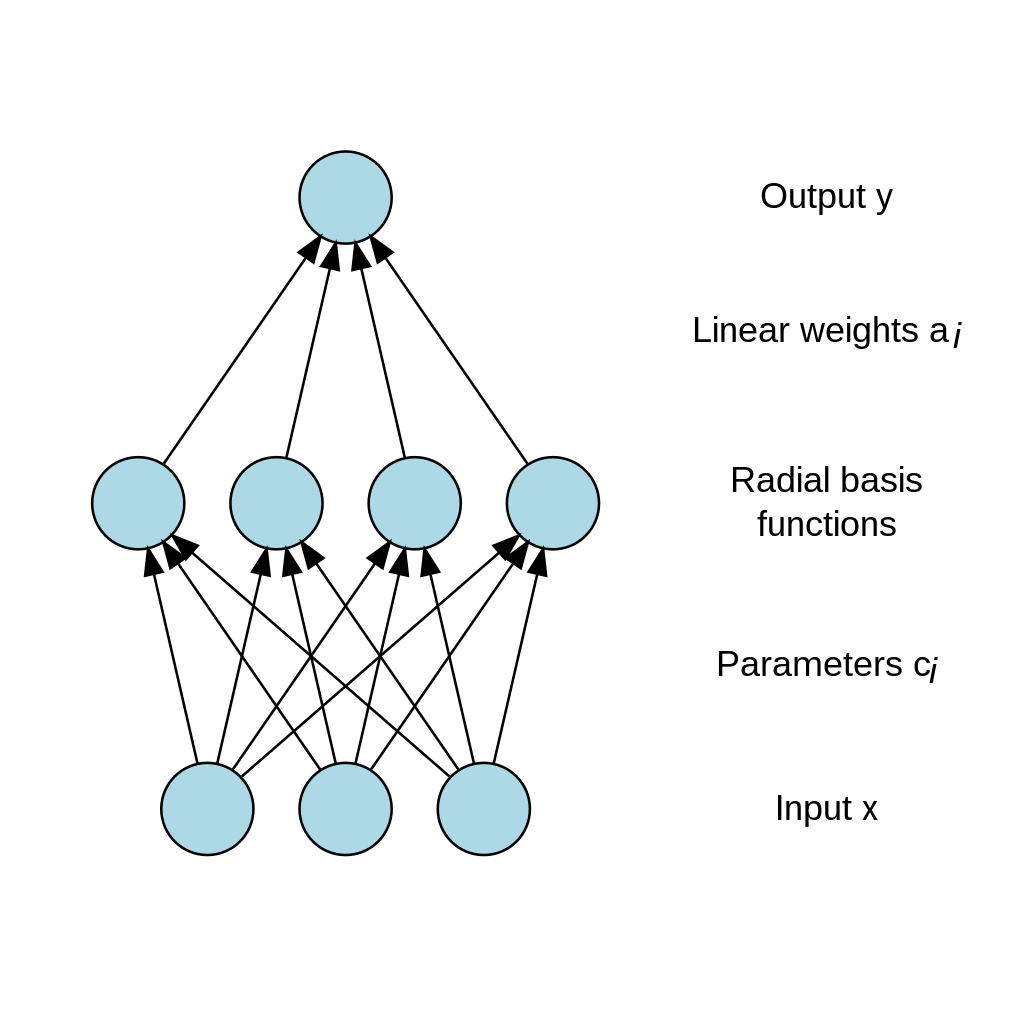
\includegraphics[width=0.6\textwidth]{./RBF.png} % Adjust the width as needed
\end{figure}
So the full equation defining our RBF network is:

\[\phi(x) = \sum_{i=1}^N a_i \rho(||x - c_i||)\]

Where the norm is typically euclidean distance and the basis function \(\rho\) is typically gaussian. \(c_i\) is the center vector for neuron \(i\) (\(c_i \in \mathbb{R}^d\) if we have d features) and \(a_i\) is the weight for the neuron \(i\). Note that because our layer is fully connected each neuron get the entirety of our input sample \(x \in \mathbf{R}^d\). Also, note that RBF Networks consist of a single hidden layer \(n\) RBF kernels, one for each neuron.

\subsection{Training}
Training typically occurs in 2 steps:
\begin{enumerate}
\item: In the first step, we find the center vectors \(c_i\) for the RBF functoins of each neuron. This can be performed in several ways: centers can be randomly sampled from some set of examples, or they can be determined by k-means clustering or something else. Note that this step is unsupervised!
\item: The second step fits a linear model with coefficients \(w_i\) to the hidden layers outputs with respect to some objective functoin. We can use gradient descent, but a more common approach is to simply solve using linear algebra. For example, let's say we want to do least squares regression. Our cost functoin is 
\[J(w) = ||\Phi w = y ||^2 = (\Phi w - y)^T(\Phi w - y) = (\Phi w)^T\Phi w - 2y^T\Phi w + y^Ty\]

Where \(\Phi\) is the ouput from our RBF, w represents the weights, and y represents the ground truth answers. If we take the derivative with respect to w and set equal to 0 will give us the extrema, which in the case of least squares gives us the set of weights that minimize the square error:

\[\frac{\partial}{\partial w}J(w) = 2\Phi^T\Phi w - 2\Phi^Ty = 0\]

Solving for this gives us the weights for our RBF:

\[w = (\Phi^T\Phi)^{-1}\Phi^Ty\]

So rather than doing gradient descent here, we can simply calculate the weights with linear algebra. Because of this, training is performed in one pass over all observed data samples.

\end{enumerate}

\subsection{When to use}
\begin{enumerate}
\item \textbf{Small to medium sized dataset}: when larger deep models might overfit, rbfs can still be useful
\item \textbf{RTOS}: RBFs can be useful on real time systems where predictions need to be made rapidly
\item \textbf{Problems with well-defined, stable features} 
\end{enumerate}
\subsection{When not to use}
\begin{enumerate}
\item \textbf{When Scalability Matters}: RBFs become computationally expensive as the number of datapoints grows. they're less scalable than modern deep learning approaches
\item \textbf{High Dimensional Data}: Severely struggle with high dimensoinal data. volume of input space increases exponentially with the number of dimensoins, requiring exponentially more data to maintain the same level of performance.
\item \textbf{Generalization in complex domains}: Don't do a good job with tasks involving complex patterns or hierarchies, such as language processing, image recognition, or something like that (if deep learning does it well, RBFs don't). 
\end{enumerate}



\section{Principal Component Analysis (PCA)}

Principal Component Analysis (PCA) is a dimensionality reduction technique that transforms a set of possibly correlated variables into a set of linearly uncorrelated variables called principal components.

\subsection{What It Is}
PCA is used to reduce the dimensionality of large datasets, improving interpretability while minimizing information loss.

\subsection{How It Works}
The PCA process involves several key mathematical steps:

\begin{enumerate}
	\item \textbf{Z-Score Standardize Data} PCA is sensitive to variances of different variables, so all variables must have mean of 0, variance of 1. For each feature \(X_i\), the standardized value \(Z_i\) is computed as \[ Z_i = \frac{X_i - \mu_i}{\sigma_i}\]
    \item \textbf{Compute the Covariance Matrix}: The Covariance matrix expresses the covariance (correlation) between each pair of features. for features \(Z_1\) and \(Z_2\), their covariance is given by \[Cov(Z_1,Z_2) = \frac{1}{M-1} \sum_{i \in M} (Z_{1,i} - \mu_{Z_1})(Z_{2,i} - \mu_{Z_2})\]
where M is the number of features. This would be a single entry in the covariance matrix:
\[ \Sigma = 
\left[
\begin{array}{cccc}
\text{Var}(Z_1) & \text{Cov}(Z_1, Z_2) & \cdots & \text{Cov}(Z_1, Z_m) \\
\text{Cov}(Z_2, Z_1) & \text{Var}(Z_2) & \cdots & \text{Cov}(Z_2, Z_m) \\
\vdots & \vdots & \ddots & \vdots \\
\text{Cov}(Z_m, Z_1) & \text{Cov}(Z_m, Z_2) & \cdots & \text{Var}(Z_m) \\
\end{array}
\right]
\]

The covariance matrix for a dataset with m features is an \( m \times m \) matrix where each element \((Z_i,Z_j)\) represents the covariance between  \(Z_i\) and \(Z_j\)  

This means that each eigenvector has length \(m\), which directly corresponds to the number of features in the dataset. The number of eigenvectors you get from PCA will also match the dimensionality of the original data set, which means you will have as many eigenvectors as there are features in your data. If your data has \(m\) features, you will compute \(m\) eigenvectors. This is because in \(m\)-dimensional space, \(m\) orthogonal vectors are needed to form an orthonormal basis for (i.e, to span) the space. Each orthogonal vector adds. If you had fewer than \(m\) vectors, you wouldn't be able to generate all possible vectors in your space. If you had more than \(m\), at least one vectory would be linearly dependent on the others and thus wouldn't form a basis (a requirement of a basis is that all vectors forming the basis must be linearly independent). 

\subsubsection{Why Eigenvectors point in direction of Maximum Variance}
The goal is to find a direction (a unit vector \(v\) into which to project the data so that the variance of hte projected data is maximized (if variance is maximized, then we have retained as much of the information that goes into explaining the spread of our data, and hence as good a representation of the original data, as possible). Projecting a matrix \(X\) in the direction of a vector is denoted as this: 

\[ v^T X v\]

imagine we want to project our covariance matrix \(\Sigma\) in some direction (any direction), but that \(v\) has to be a unit vector. We have:
\[ v^T \Sigma v, v^T v = 1\]
This is now an optimization problem. If we apply Lagrange multipliers to this optimization problem: \[argmax_{v \in \mathbb{R}^m} v^T \Sigma v\] We end up with \[\Sigma v = \lambda v\] Where \(\lambda\) is some constant. This is EXACTLY the definition of the eigenvectors of \(\Sigma\), thus proving that the eigenvectors point in the directions that maximize the variance of the data

\textbf{Detailed steps of proof are here:}


Given the optimization problem to maximize $v^T \Sigma v$ under the constraint $v^T v = 1$, where $\Sigma$ is the covariance matrix, and $v$ is the vector upon which the data is projected:

Introduce a Lagrange multiplier $\lambda$ to handle the constraint, and define the Lagrangian function $L$ as:
\[ L = v^T \Sigma v - \lambda (v^T v - 1) \]

To find the maximum, take the gradient of $L$ with respect to $v$ and set it equal to zero. The derivative with respect to the constraint variable $\lambda$ will naturally enforce the constraint. The gradient of the Lagrangian with respect to $v$ is:
\[ \frac{\partial L}{\partial v} = 2\Sigma v - 2\lambda v = 0 \]


This step assumes that $\Sigma$ is symmetric, which is typically the case for covariance matrices. 
We can rewrite the partial derivative as 
\[ (\Sigma - \lambda I)v = 0 \] 

This is the definition of the eigenvectors of \(\Sigma\)! Therefore the eigenvectors must point in the direction of maximum variance for the data.


    \item \textbf{Perform Eigendecomposition on the Covariance Matrix}: Solve \(Av = \lambda v\) for a \(2 \times 2\) matrix \(A = \begin{pmatrix} a & b \\ c & d \end{pmatrix}\), leading to eigenvalues \(\lambda\) by solving \(\det(A - \lambda I) = 0\), where \(I\) is the identity matrix.
    \item \textbf{Sort Eigenvectors According to the Eigenvalues}: Eigenvectors are sorted by decreasing eigenvalues. Eigenvalues represent the variance captured by each principal component.
    \item \textbf{Select Principal Components}: This can be done by looking at the cumulative explained variance ratio, which is the sum of the eigenvalues of the selected principal components divided by the sum of all eigenvalues. Typically, you choose the smallest number of principal components that still accounts for a large portion of the variance (common thresholds are 90\%, 95\%, etc.).
	\item \textbf{Transform original dataset} Form matrix from chosen eigenvectors. If you keep \(k\) principal components, your projection matrix \(W\) will be of size \(m \times k\), where m is the number of original features. Then multiply your Z-score-standardized dataset by this matrix to project it in the direction of your components.
\end{enumerate} 

\subsection{When to Use / When Not to Use}
\textbf{When to Use:}
\begin{itemize}
    \item For exploratory data analysis and understanding data structure.
    \item To reduce variables and preserve information.
    \item Before applying machine learning models to reduce computation and avoid overfitting.
\end{itemize}

\textbf{When Not to Use:}
\begin{itemize}
    \item When variance does not imply importance.
    \item If data is not linearly correlated.
    \item To capture non-linear patterns in data.
\end{itemize}

\subsection{Pros / Cons}
\textbf{Pros:}
\begin{itemize}
    \item Simplifies data complexity, aiding in visualization and understanding.
    \item Identifies and removes redundant features.
    \item Can improve machine learning algorithm performance by reducing overfitting.
\end{itemize}

\textbf{Cons:}
\begin{itemize}
    \item Principal components not interpretable.
    \item Only captures linear relationships in data
	\item If important information doesn't manifest as high-variance, it will be neglected
\end{itemize}
\section{Floating Point Values \& Binary}
So many ML engineers don't know binary, because they forgot it after college. It's really important you know this.\\

All decimal numbers can be represented as strings of 1's and 0's. Everyone knows this. This is binary. 
\[
3.1416_{10} = 0100001001001000
\]
IEEE Floating Point Values (the most common floating-point representations of binary) are broken down into 3 components: a sign, an exponent, and a decimal (called the mantissa):
\[
\underbrace{0}_{\text{Sign}} \,\, | \,\, \underbrace{10000}_{\text{Exponent}} \,\, | \,\, \underbrace{1001001000}_{\text{Mantissa}}
\]

All numbers can be represented as IEEE FP binary given enough digits (bits) of precision. Common precisions to use are 8-bit, 16-bit (half precision), 32-bit (full precision), and 64-bit (double precision). This shows the range of numbers (and digits of pi) you can represent with each.
\begin{table}[h]
    \centering
    \resizebox{\textwidth}{!}{%
    \begin{tabular}{|c|c|c|c|c|c|}
        \hline
        \textbf{Precision} & \textbf{Range} & \textbf{Exponent Bits} & \textbf{Mantissa Bits} & \textbf{Bias} & \textbf{Pi Approximation} \\
        \hline
        \textbf{FP8}       & $[-240, +240]$ & 4                      & 3                      & 8            & 3.14 \\
        \hline
        \textbf{FP16}      & $[6.1 \times 10^{-5}, 6.5 \times 10^4]$ & 5                      & 10                     & 16            & 3.14060 \\
        \hline
        \textbf{FP32}      & $[1.4 \times 10^{-45}, 3.4 \times 10^{38}]$ & 8                      & 23                     & 128           & 3.1415927 \\
        \hline
        \textbf{FP64}      & $[5.0 \times 10^{-324}, 1.8 \times 10^{308}]$ & 11                     & 52                     & 1024          & 3.141592653589793 \\
        \hline
    \end{tabular}%
    }
    \caption{Common IEEE Floating-Point Precisions and Approximations of Pi}
\end{table}

\subsection{Calculating Binary}
For IEEE FP8 e4m3 (exponent 4 mantissa 3) encoding of Pi.\\
\begin{itemize}
\item \textbf{Sign}: 0th bit (left-most) gets set to 0 for positive numbers, 1 for negative numbers
\item \textbf{Exponent}: Binarize the exponent: \(3 = 00011\). 
\item \textbf{Mantissa}: Use this algorithm to get the binary mantissa: Take the fractional value \((0.14)\) and multiply by 2. If the result is greater than 1, add a 1 bit to mantissa and then subtract 1 from the result. If the result is less than 1, then add 0 bit to mantissa. Repeat until you reach the maximum number of bits for the mantissa or get to 0.
\item Example:
\[0.14 \times 2 = 0.28 \rightarrow \text{encode } 0\]
\[0.28 \times 2 = 0.56 \rightarrow \text{encode } 0\]
\[0.56 \times 2 = 1.12 \rightarrow \text{encode } 1\]
\[(1.12 - 1 = 0.12)\]
\[0.12 \times 2 = 0.24 \rightarrow \text{encode } 0\]
\item \textbf{Shifting by Bias}: Right now we have \(3.14 = 11.0010\). Shift this to \(1.1001 \times 2^1\). Our mantissa is \(1001\) (There's an implicit leading 1) and our exponent is \(2^{1 + \text{bias}}=2^{1+8} = 2^9\)
\item \textbf{Final Binary Representation}: \(1 \quad 1001 \quad 100 \) (we lost the final 1 bit due to truncation).
\end{itemize}
\subsection{Calculating Decimal from Binary}
So at this point we have \(0 \quad 1001 \quad 001\) for our fp8 e4m3 encoding of pi. To back out our result for this, we do \[\text{sign} \cdot 2^{\text{exponent} - \text{bias}} \cdot 1.\text{decimal}\]
\[+1 \cdot 2^{9-8} \cdot 1.100_2 = 2 \times 1\frac{1}{2} = 3.0\]
\section{Singular Value Decomposition (SVD)}
SVD is a fundamental dimensionality reduction technique that is every bit as important as Principal Component Analysis and Fischer's Linear Discriminant. Given a matrix \(A\) of shape (\(m, n\))— \(m\) samples and \(n\) features— we decompose \(A\) into the following matrices:

\[A = U\Sigma V^T\]

Where
\begin{itemize}
\item \(U = \text{eig}(AA^T)\) and has shape \(m \times m\). Its columns are the eigenvectors of \(AA^T\). In the eigenfaces example, each column corresponds to an eigenface. The 0th column represents the most important singular value, and their importance decreases left to right.
\item \(V = \text{eig}(A^TA)\) and has shape \(n \times n\). In the eigenfaces example, each column of \(V\) (note it's \(V^T\) in the original equation and \(V\) now, so this would be each row of \(V^T\)) represents the specific mixture of the \(m\) left singular vectors that produce each sample. So column 0 gives the mixture of the columns of \(U\Sigma\) that produce the 0th sample in our original matrix \(A\), column 1 gives the mixture for the 1st sample, and all the way up to column \(n\) which gives the mixture for the \(n\)th sample.
\item \(\Sigma\): A \(m \times n\) diagonal matrix of non-negative real numbers that represent the energy associated with each column in \(U\) and each row in \(V\). It decreases left to right. This matrix gives the square root of the eigenvalues of \(AA^T\) and \(A^TA\) (note that \(AA^T\) and \(A^TA\) will have the same eigenvalues, and if they have different numbers of eigenvectors, then any additional eigenvalues one has but not the other are 0).
\end{itemize}

\subsection{Performing SVD Example}

Given the matrix:
\[
A = 
\begin{bmatrix}
1 & 2 & 3 \\
4 & 5 & 6
\end{bmatrix}
\]

We calculate the following:

\[
AA^T =
\begin{bmatrix}
14 & 32 \\
32 & 77
\end{bmatrix},
\quad
A^TA =
\begin{bmatrix}
17 & 22 & 27 \\
22 & 29 & 36 \\
27 & 36 & 45
\end{bmatrix}
\]

The eigenvalues and eigenvectors of these matrices are:

For \(AA^T\):
\[
\text{Eigenvalues: } \{0.59732747, 90.4026725\}
\]
\[
\text{Eigenvectors: }
\begin{bmatrix}
-0.3863177 & 0.92236578 \\
-0.92236578 & -0.3863177
\end{bmatrix}
\]

For \(A^TA\):
\[
\text{Eigenvalues: } \{0.59732747, 90.4026725, 0\}
\]
\[
\text{Eigenvectors: }
\begin{bmatrix}
-0.42866713 & -0.80596391 & 0.40824829 \\
-0.56630692 & -0.11238241 & -0.81649658 \\
-0.7039467 & 0.58119908 & 0.40824829
\end{bmatrix}
\]

Using these, we construct:

\[
\Sigma =
\begin{bmatrix}
9.508032 & 0 & 0 \\
0 & 0.77286964 & 0
\end{bmatrix}
\]
\textit{(Notice we take the square root of the nonzero eigenvalues and populate the diagonals)}.
\[
U =
\begin{bmatrix}
-0.3863177 & 0.92236578 \\
-0.92236578 & -0.3863177
\end{bmatrix},
\quad
V =
\begin{bmatrix}
-0.42866713 & -0.80596391 & 0.40824829 \\
-0.56630692 & -0.11238241 & -0.81649658 \\
-0.7039467 & 0.58119908 & 0.40824829
\end{bmatrix}
\]

Finally, reconstructing \(A\):
\[
A \approx U \Sigma V^T =
\begin{bmatrix}
1 & 2 & 3 \\
4 & 5 & 6
\end{bmatrix}
\]


\subsection{When to use SVD vs. PCA}

While SVD and PCA are mathematically related, their applications differ based on the nature of the data and the specific goals of the analysis:

\textbf{Principal Component Analysis (PCA):}
- \emph{Dimensionality Reduction:} PCA is particularly useful for reducing the number of features in high-dimensional data while retaining as much variance as possible.
- \emph{Feature Extraction:} PCA can identify the principal components that capture the most significant variance in the data, which can be used as new features for further analysis.
- \emph{Noise Reduction:} By retaining only the principal components with the highest variance, PCA can help remove noise from the data.
- \emph{Visualization:} PCA is often used to project high-dimensional data into 2D or 3D space for visualization purposes.

\textbf{Singular Value Decomposition (SVD):}
- \emph{Matrix Factorization:} SVD is essential for decomposing a matrix into its constituent components, useful in collaborative filtering for recommendation systems.
- \emph{Latent Semantic Analysis (LSA):} SVD is used in LSA to uncover the latent relationships between terms and documents in text mining.
- \emph{Data Imputation:} SVD can be used to fill in missing values in a matrix by approximating the missing entries using the known values and the latent structure captured by SVD.
- \emph{Low-Rank Approximation:} SVD is useful for finding low-rank approximations of matrices, which can reduce storage and computational requirements in applications such as image compression.

In summary, use PCA when your goal is to reduce dimensionality and retain the maximum variance, and use SVD when you need to factorize a matrix to uncover latent structures or perform tasks like data imputation and recommendation.

\subsection{Example Application of SVD}
\textbf{Problem}: Design a recommendation system for Spotify using SVD. \\
\textbf{1. Create the User-Song Matrix}
You can approach this problem by leveraging a user-song interactoin matrix:
\begin{itemize}
\item Assume you have \(m\) users and \(n\) songs.
\item Construct a matrix \(A\) of size \(m \times n\) where \(A[i][j]\) represents the number of times user \(i\) played song \(j\) or the rating they gave the song if available
\item If user \(i\) hasn't played song \(j\), set  \(A[i][j] = 0\) 
\end{itemize}

For example:
\[
A = 
\begin{bmatrix}
5 & 3 & 0 & 1 \\
4 & 0 & 0 & 1 \\
1 & 1 & 0 & 5 \\
0 & 0 & 5 & 4 \\
0 & 0 & 4 & 0 \\
\end{bmatrix}
\]

% insert A you gave here
\textbf{2. Apply SVD}\\
Decompose \(A\) into \(U\Sigma V^T\)\\
Where
\begin{itemize}
\item \(U\) is an \(m \times m\) matrix of left singular vectors (user preferences, \(AA^T\))
\item \(\Sigma\) is a diagonal matrix of singular values (weights for the features)
\item \(V^T\) is an \(n \times n\) matrix of right singular vectors (song features, \(A^TA\))
\end{itemize}

\textbf{3. Build Reduced Rank Approximation of A}\\
\begin{itemize}
\item The dimensions of the reduced matrices are:
    \begin{itemize}
    \item \(U_k\): \(m \times k\) (\(5 \times 2\)).
    \item \(\Sigma_k\): \(k \times k\) (\(2 \times 2\)).
    \item \(V_k^T\): \(k \times n\) (\(2 \times 4\)).
    \end{itemize}
\end{itemize}
% what would the dimensions of the three reduced rank matrices be? 

% insert reconstructed matrix here
\[
A_k = 
\begin{bmatrix}
5.02 & 2.99 & 0.12 & 0.98 \\
4.11 & 2.48 & 0.07 & 1.01 \\
0.97 & 1.06 & 4.68 & 4.81 \\
0.03 & 0.21 & 5.13 & 4.12 \\
0.06 & 0.18 & 4.02 & 0.24 \\
\end{bmatrix}
\]
\textbf{4. Make Recommendations}\\
For each user, identify the songs with the highest predicted scores in \(A_k\) that they have not already played. 

\textbf{Questions / Specifications}\\
Let's say I have a specific user I want to create recommendations for. I would identify \(m-1\) similar users to them using some other analysis. Then I would identify \(n\) songs which are a mixture of their most played songs and similar songs (similarity determined by a third semantic analysis method) that they have not played before. I would then construct the matrix from those \(m\) users and \(n\) songs. 

\section{L1 Norm / Loss and L2 Norm / Loss}

The L1 norm and L2 norm are two different ways of measuring the size (or length) of a vector, and they have corresponding loss functions that are used in optimization problems, including machine learning.

\subsection{L1 Norm (Manhattan Norm)}
The L1 norm of a vector \( \mathbf{x} = [x_1, x_2, \ldots, x_n] \) is the sum of the absolute values of its components:
\[ ||\mathbf{x}||_1 = \sum_{i=1}^{n} |x_i| \]
It is also known as the Manhattan norm or taxicab norm.

\subsection{L2 Norm (Euclidean Norm)}
The L2 norm of a vector \( \mathbf{x} \) is the square root of the sum of the squares of its components:
\[ ||\mathbf{x}||_2 = \sqrt{\sum_{i=1}^{n} x_i^2} \]
It is also known as the Euclidean norm because it measures the straight-line distance between two points in Euclidean space.

\subsection{Relationship Between L1 and L2 Norms}
The L1 and L2 norms satisfy norm properties, such as non-negativity, definiteness, and the triangle inequality. L2 norm is more influenced by large values or outliers due to squaring the components, whereas the L1 norm is robust against outliers.

\subsection{L1 Loss (MAE)}
The L1 loss is defined as the sum of the absolute differences between the predicted and actual values and encourages sparsity in the solution:
\[ L_1(\mathbf{y}, \mathbf{\hat{y}}) = \sum_{i=1}^{m} |y_i - \hat{y}_i| \]
Where m is the number of dimensions in the data. If we want to average this loss across \(N\) samples, then we have MAE:

\[ \text{MAE} = \frac{1}{N} \sum_{j=1}^{N}  \sum_{i=1}^{m} |y_{ij} - \hat{y}_{ij}| \]

Where \(j\) is the \(j^{th}\) sample and \(i\) is the \(i^{th}\) dimension of that sample

\subsection{L2 Loss (MSE)}
The L2 loss is the sum of the squares of the differences and is sensitive to outliers, but computationally efficient for optimization due to its differentiable nature:
\[ L_2(\mathbf{y}, \mathbf{\hat{y}}) = \sum_{i=1}^{m} (y_i - \hat{y}_i)^2 \]

If we want to average this loss across \(N\) samples, then we have MSE:
\[ \text{MSE} = \frac{1}{N} \sum_{j=1}^{N}   \sum_{i=1}^{m} (y_{ij}- \hat{y}_{ij})^2  \]

Where \(j\) is the \(j^{th}\) sample and \(i\) is the \(i^{th}\) dimension of that sample\\

Both loss functions have applications in machine learning, with L1 loss being used for models where feature selection is important, and L2 loss being common in regression problems. L1 loss is less sensitive to outliers. 
\subsection{Why \( L_1 \) Loss Encourages Sparsity}
The \( L_1 \) loss, defined as \( L_1(\mathbf{w}) = \sum_{i=1}^n |w_i| \), applies a constant gradient of \( \pm 1 \) for non-zero parameters \( w_i \). During gradient descent, each update for parameter \( w_i \) is given by:
\[
w_i = w_i - \eta \, \text{sign}(w_i)
\]
where \( \eta \) is the learning rate. For small \( w_i \), if \( |w_i| \leq \eta \), this step can drive \( w_i \) to zero in a single update, promoting sparsity. In contrast, \( L_2 \) loss, defined as \( L_2(\mathbf{w}) = \sum_{i=1}^n w_i^2 \), produces gradients proportional to the parameters \( w_i \), resulting in smaller changes for small values:
\[
w_i = w_i - \eta \cdot 2 w_i
\]
This leads to a gradual reduction without promoting sparsity as effectively as \( L_1 \) loss.

\subsection{When to use}
\subsubsection{Feature Selection in High-Dimensional Data}
\begin{itemize}
    \item \textbf{Task:} Building a predictive model in a high-dimensional space where many features may be irrelevant or redundant.
    \item \textbf{Use of L1 Loss:} Utilize L1 loss (Lasso regression) which encourages sparsity in the model parameters. This can lead to models where some feature weights are exactly zero, effectively performing feature selection and helping to identify the most important features.
\end{itemize}
\subsubsection{Predicting Continuous Outcomes with Normally Distributed Errors}
\begin{itemize}
    \item \textbf{Task:} Regression analysis where the goal is to predict continuous outcomes and the errors are assumed to be normally distributed.
    \item \textbf{Use of L2 Loss:} Apply L2 loss (Ridge regression) which minimizes the sum of the squared differences between the predicted and actual values. This approach is sensitive to outliers but provides stable and well-behaved solutions when errors are Gaussian.
\end{itemize}

\section{Retrieval Augmented Generation (RAG)}
Retrieval Augmented Generation (RAG) is a framework that combines the strengths of LLMs and information retrieval systems to enhance the ability of LLMs to generate contextually accurate and detailed responses in specific domains. Its purpose is to improve LLMs' ability to generate good domain-specific content without incurring the significant computational cost of fine-tuning the LLM.\\

Given an input space \(\mathcal{X}\), a knowledge corpus \(\mathcal{K}\), and an output space \(\mathcal{Y}\), the task is to accept an input \(x \in \mathcal{X}\) and generate an output \(y \in \mathcal{Y}\) such that \(y\) is semantically aligned with \(x\) and consistent with the information in \(\mathcal{K}\). A RAG system does this with three components:
\begin{itemize}
\item \textbf{A Knowledge Corpus}: \(\mathcal{K}\)
\item \textbf{A Retriever}: Some (typically) transformer-based architecture like BERT
\item \textbf{A Generator}: An LLM whose performance we want to fine-tune
\end{itemize}
We learn a set of vectorized embeddings \(\psi(d)\) for each item \(d\) in our knowledge corpus (the retriever learns these embeddings). Then at inference time, the retriever computes the cosine similarity of the embedded input \(\phi(x)\) against each of the embeddings \(\psi(d)\). Then it selects the top \(k\) embeddings and returns them as natural language inputs to the generator. The actual input \(x\) is then concatenated with the \(k\) most relevant documents, and all are passed through the LLM for generation.

\subsection{Learning Process}
The whole point of RAG is avoiding fine-tuning the LLM (the generator). So all learning is done by the retriever. \\

The retriever is typically a smaller transformer-based model like BERT. The retriever learns by a supervised learning process using contrastive loss. In each iteration, a single query \(x\), a single relevant document \(d^+\), and several irrelevant documents \(d^-_i \in d^-\) are passed to BERT:

\[
\mathcal{L}_{\text{contrastive}} = -\log \frac{e^{\text{sim}(\phi(x), \psi(d^+))}}{e^{\text{sim}(\phi(x), \psi(d^+))} + \sum_{d^-} e^{\text{sim}(\phi(x), \psi(d^-))}}
\]

Notice that the inputs \(x\) and the documents \(d\) may have different embedding functions (they can and often do, but don't have to). This is because documents \(d\) are often longer and highly structured, while inputs \(x\) are likely to be shorter and less structured. They likely have very different distributions. \\

The \(\text{sim}\) function is given by cosine similarity:

\[
\text{sim}(\phi(x), \psi(d)) = \frac{\phi(x) \cdot \psi(d)}{\|\phi(x)\| \|\psi(d)\|}
\]

The idea behind the loss function is that the larger the distance between \(\phi(x)\) and \(\psi(d^-)\), the smaller the loss will get. Also notice that because of the exponential, the summation will never reach 0, and therefore following the gradient will lead us to the desired behavior. \\

The retrieved documents \(D\) are typically in natural language format (or some other notation that the model already learned to process during the pretraining process, like math), and we simply pass all these documents through the LLM.

\section{Triplet Loss}
Triplet loss is a loss function for machine learning algorithms where a reference input (called anchor) is compared to a matching input (called positive) and a non-matching input (called negative). The distance from the anchor to the positive is minimized, and the distance from the anchor to the negative input is maximized. This loss is, along with Contrastive Loss, are the two loss functions commonly used to train Siamese Networks.

\subsection{Mathematical Formulation}
Triplet Loss is defined via the Euclidean Distance Function:
\[\mathcal{L}(A, P, N) = \max (|| f(A) - f(P)||_2 - || f(A) - f(N) ||_2 + \alpha, 0)\]

Where \(|| ... ||_2\) denotes the Euclidean Norm. The idea here is that anchor image \(A\) and the positive image \(P\) should be of the same class, while \(A\) and \(N\) will be of different classes. We want  \(f(A) \approx f(P)\) and \(f(A) != f(N)\). If that is the case, then there will be 0 loss. The hyperparameter \(\alpha\) is the minimum difference required between \(|| f(A) - f(P)||_2\) and \( || f(A) - f(N) ||_2\) for us to consider a triplet correctly classified. \(\alpha\) is important because it forces the network to create a more significant separation between positive and negative classes. Without this, a network could learn a 0 loss scenario in which the positive sample is only infinitesimally more different from the anchor than the negative sample. This isn't what we would want. 
\subsection{Example Application}
An example application of this would be in Siamese networks. We could train a Siamese network to do facial recognition, and use triplet loss to train the network such that embeddings of similar faces are close, and dissimilar faces are far apart.
\section {Precision And Recall}
Precision and recall are performance metrics used to evaluate the relevance of the results returned by a system. Precision is True Positives as a fraction of all positives (TP + FP). Recall is True Positives as a fraction of all ground truth positive instances (TP + FN).

\subsection{Precision}
\textbf{Definition:} Precision, also known as the positive predictive value, is the ratio of true positive results to the total number of positive results. It answers the question, "Of all the instances classified as positive, how many are actually positive?"

\textbf{Mathematical Formula:}
\[ \text{Precision} = \frac{TP}{TP + FP} \]
where \(TP\) (True Positives) are the instances correctly predicted as positive, and \(FP\) (False Positives) are the instances incorrectly predicted as positive.

\subsection{Recall}
\textbf{Definition:} Recall, also known as sensitivity, is the ratio of true positive results to the total number of instances that were actually positive. It answers the question, "Of all the actual positive instances, how many did we get right?"

\textbf{Mathematical Formula:}
\[ \text{Recall} = \frac{TP}{TP + FN} \]
where \(TP\) (True Positives) are as defined above, and \(FN\) (False Negatives) are the instances that were incorrectly predicted as negative despite being positive.

\section {Jensen-Shannon Divergence (JSD)}
The Jensen-Shannon Divergence (JSD) is a symmetric and smoothed measure of the similarity between two probability distributions, often used when the true distribution is unknown or to compare distributions in a more stable manner than the Kullback-Leibler (KL) divergence.

\subsection{How It Works}

Jensen-Shannon Divergence is defined as follows:
\begin{enumerate}
    \item Calculate the average distribution \(M\) between \(P\) and \(Q\):
    \[ M = \frac{1}{2}(P + Q) \]
	So if P and Q are N(2,1) and N(3,1) respectively, then M will be the sum of these two gaussian distributions divided by 2 to ensure it remains a valid PDF
    \item Compute the KL divergence to \(M\) from both \(P\) and \(Q\):
    \[ D_{KL}(P || M) = \sum_{x} P(x) \log\left(\frac{P(x)}{M(x)}\right) \]
    \[ D_{KL}(Q || M) = \sum_{x} Q(x) \log\left(\frac{Q(x)}{M(x)}\right) \]
    \item The JSD is then the average of these two KL divergences:
    \[ JSD(P || Q) = \frac{1}{2} D_{KL}(P || M) + \frac{1}{2} D_{KL}(Q || M) \]
\end{enumerate}
\subsection{When to Prefer JSD over KLD}

\begin{itemize}
    \item \textbf{Symmetric Comparisons:} JSD is preferred for symmetric measures of divergence, useful in clustering or similarity analysis where the order of comparison does not matter. 
	\item \textbf{Example:}  In clustering or similarity analysis of text documents represented by topic distributions, where the goal is to measure how similar two documents are, irrespective of the order.
    
    \item \textbf{Handling Non-Overlapping Supports:} JSD is suitable for comparing distributions with non-overlapping supports without infinite divergence issues. 
    \item \textbf{Example:} In generative model evaluation, such as comparing the distribution of generated images to real images in GANs, where some pixels might have values in one distribution not present in the other.
    
    \item \textbf{Smoothed Measure for Stability:} JSD provides a smoothed and stable measure, ideal for comparing sparse distributions. 
	\item \textbf{Example:}  In bioinformatics, for comparing gene expression profiles across different conditions where the data might be sparse, and a stable measure of similarity is required.
\end{itemize}

\subsection{When to Prefer KLD over JSD}

\begin{itemize}
    \item \textbf{Relative Entropy for Information Loss:} KLD is useful for measuring the information loss when approximating one distribution with another, emphasizing asymmetry. \textit{Example:} In model compression or pruning, where KLD can measure how much information is lost when the detailed model’s distribution is approximated by a simpler model.
    
    \item \textbf{Specific Directional Measure:} KLD's asymmetry is valuable when the direction of divergence is important, such as in model calibration. \textit{Example:} In machine learning model calibration, where KLD can quantify how the predicted probability distribution of a classifier diverges from the empirical distribution of the true labels.
    
    \item \textbf{Optimization in Variational Inference:} KLD is essential in variational inference for approximating complex posterior distributions. \textit{Example:} In training Variational Autoencoders (VAEs), KLD is used to regularize the encoder by measuring the divergence between the encoded latent variable distributions and a prior distribution, typically a Gaussian. (kld is necessary because its asymmetricity here is necessary for VAEs). 
\end{itemize}
\section{Logistic Regression}

Logistic Regression is a statistical model and a fundamental algorithm in machine learning, used for classification tasks, that predicts the probability that a given input belongs to a certain category.

\subsection{Mathematical Formulation}

The logistic regression model predicts the probability \( P(Y=1|X) \) that an instance \( X \) belongs to the class \( Y=1 \), based on a logistic function of a linear combination of the input features:

\[ P(Y=1|X) = \frac{1}{1 + e^{-(\beta_0 + \beta_1 X_1 + \dots + \beta_n X_n)}} \]

Here, \( \beta_0, \beta_1, \ldots, \beta_n \) are the parameters of the model, \( X_1, \ldots, X_n \) are the features, and \( e \) is the base of the natural logarithm.

\subsection{Learning the Parameters}

Parameters of a logistic regression model are estimated using maximum likelihood estimation (MLE). The goal is to find the parameter values that maximize the likelihood of the observed set of labels given the input features, which is equivalent to minimizing the negative log-likelihood, or cross-entropy loss, over the training data:

\[ \mathcal{L}(\beta) = -\sum_{i=1}^{m} [y_i \log(p_i) + (1 - y_i) \log(1 - p_i)] \]

where \( m \) is the number of instances, \( y_i \) is the label of the \( i \)-th instance, and \( p_i \) is the predicted probability \( P(Y=1|X_i) \) for that instance.

\subsection{Why It Works}

Logistic regression works well for binary classification because the logistic function—also known as the sigmoid function—squeezes the output of the linear model into the range (0, 1), which is interpretable as a probability. It is robust to noise around the decision boundary and naturally produces non-linear decision boundaries.

\subsection{When to Use Logistic Regression}

\textbf{When to Use}:
\begin{itemize}
    \item When the dependent variable is binary.
    \item For understanding the impact of several independent variables on a single outcome variable.
    \item When a probabilistic framework is needed for binary classification.
\end{itemize}

\textbf{Pros}:
\begin{itemize}
    \item Provides probabilities for outcomes.
    \item Can be regularized to prevent overfitting.
    \item Efficient and easy to implement.
    \item Interpretable model with feature importance directly given by the coefficients.
\end{itemize}

\textbf{Cons}:
\begin{itemize}
    \item Assumes linear decision boundary, which may not be adequate for all problems.
    \item Can be outperformed by more complex models for non-linear problems.
    \item Sensitive to imbalanced datasets.
\end{itemize}

Logistic regression is particularly useful for problems where it is beneficial not only to predict outcomes but also to understand the influence of the features. However, it is not suitable for all datasets, especially those with complex, non-linear relationships.

\section{Mahalanobis Distance}

Mahalanobis distance is a multivariate measure of distance that takes into account the correlations between different variables in the dataset. It provides a way to determine the distance between a point and a distribution, or between two points in space controlled by the distribution's scale and correlation.

\subsection{Mathematical Definition}

The Mahalanobis distance \(D\) between a point \( \mathbf{x} \) and a set of points with mean \( \boldsymbol{\mu} \) and covariance matrix \( \mathbf{S} \) is defined as:

\[ D(\mathbf{x}) = \sqrt{(\mathbf{x} - \boldsymbol{\mu})^T \mathbf{S}^{-1} (\mathbf{x} - \boldsymbol{\mu})} \]

Here, \( \mathbf{x} \) and \( \boldsymbol{\mu} \) are vectors representing the point and the mean of the distribution, respectively, and \( \mathbf{S} \) is the covariance matrix of the distribution, which encapsulates information about the variance of each variable and the covariance between variables.

\subsection{Why It Works}

Mahalanobis distance works well for assessing similarity or anomaly because it accounts for the variance of each variable and the covariance between variables. Unlike Euclidean distance, which assumes orthogonal and uniformly scaled dimensions, Mahalanobis distance scales the axes according to the spread of the data and rotates them according to the correlation structure.

\subsection{When to Use Mahalanobis Distance}

\textbf{When to Use}:
\begin{itemize}
    \item In anomaly detection, to assess how anomalous a point is with respect to a distribution.
    \item For multivariate outlier detection, because it can identify outliers that are not detectable in univariate analysis due to the masking effect.
    \item In clustering algorithms, like k-means, to form clusters that account for correlation and variance in the data.
\end{itemize}

\textbf{Pros}:
\begin{itemize}
    \item Takes into account the statistical properties of the data.
    \item Is scale-invariant, i.e., independent of the scale of measurements.
    \item More accurate for datasets where variables are correlated.
\end{itemize}

\textbf{Cons}:
\begin{itemize}
    \item Computationally intensive for large datasets due to the inversion of the covariance matrix.
    \item The covariance matrix must be non-singular, which requires that there are more data points than dimensions and no perfect multicollinearity.
    \item Less interpretable compared to more straightforward metrics like Euclidean distance.
\end{itemize}

Mahalanobis distance is invaluable for applications where the underlying data is multivariate and the relationship between variables is important. It is particularly effective when working with normally distributed data or when the scale and correlation within the data need to be considered.
\section{Discrete Time Fourier Series}
The Discrete-Time Fourier Series (DTFS) is used to represent discrete, periodic time-domain signals in the frequency domain.

\subsection{Formulation}
A periodic discrete-time signal $x[n]$ with period $N$ can be expressed as:
\begin{equation}
    x[n] = \sum_{k=0}^{N-1} C_k e^{j \frac{2\pi}{N} k n},
\end{equation}
where the DTFS coefficients $C_k$ are computed as:
\begin{equation}
    C_k = \frac{1}{N} \sum_{n=0}^{N-1} x[n] e^{-j \frac{2\pi}{N} k n}.
\end{equation}
These coefficients $C_k$ form the spectral decomposition of $x[n]$ in the frequency domain, representing its discrete Fourier series.

\subsection{Example Calculation}
Consider $x[n] = \{1,2,3,0\}$ with period $N=4$. The DTFS coefficients are computed as follows:
\begin{align*}
    C_0 &= \frac{1}{4} (1 + 2 + 3 + 0) = 1.5. \\
    C_1 &= \frac{1}{4} \sum_{n=0}^{3} x[n] e^{-j \frac{2\pi}{4} (1) n} \\
        &= \frac{1}{4} \left( 1 e^{-j 0} + 2 e^{-j \pi/2} + 3 e^{-j \pi} + 0 e^{-j 3\pi/2} \right) \\
        &= \frac{1}{4} \left( 1 + 2(-j) + 3(-1) + 0(j) \right) = -0.5 - 0.5j. \\
    C_2 &= \frac{1}{4} \sum_{n=0}^{3} x[n] e^{-j \frac{4\pi}{4} n} \\
        &= \frac{1}{4} (1 e^{-j0} + 2 e^{-j\pi} + 3 e^{-j2\pi} + 0 e^{-j3\pi}) = 0. \\
    C_3 &= \frac{1}{4} \sum_{n=0}^{3} x[n] e^{-j \frac{6\pi}{4} n} \\
        &= \frac{1}{4} (1 e^{-j0} + 2 e^{-j3\pi/2} + 3 e^{-j3\pi} + 0 e^{-j9\pi/2}) \\
        &= -0.5 + 0.5j.
\end{align*}
\section{Fourier Transforms}
\subsection{Euler's Identity}
Euler's Identity is a foundational mathematical theorem that states any sinusoidal function can be expressed as a complex exponential: 
\[e^{i\pi} = -1\]
From this equation, the definitions of sine and cosine follow (in \(\Omega = \) rad/sec):

\[A\cos (\Omega_0 t + \theta) = \frac{A}{2}\left(e^{j(\Omega_0 t + \theta)} + e^{-j(\Omega_0 t + \theta)} \right)\]
\[A\sin (\Omega_0 t + \theta) = \frac{A}{2}\left(e^{j(\Omega_0 t + \theta)} - e^{-j(\Omega_0 t + \theta)} \right)\]

Where \(A\) gives the amplitude, \(\Omega_0\) gives the intial frequency in radians per second, and \(\theta\) gives the phase offset. This fundamental identity makes fourier transforms possible.
\subsection{Fourier Transforms}

Fourier Transforms and Series relate the frequency content of a signal to its time domain content. 

The Fourier domain provides a powerful way to analyze and understand signals by transforming them from the time domain to the frequency domain. This subsection covers the key relationships and transformations between these two domains.\\
The relationship between the time domain and frequency domain properties of signals can be summarized as follows:
\begin{itemize}
    \item \textbf{Aperiodic in Time} $\leftrightarrow$ \textbf{Continuous in Frequency}
    \item \textbf{Periodic in Time} $\leftrightarrow$ \textbf{Discrete in Frequency}
    \item \textbf{Continuous in Time} $\leftrightarrow$ \textbf{Aperiodic in Frequency}
    \item \textbf{Discrete in Time} $\leftrightarrow$ \textbf{Periodic in Frequency}
\end{itemize}

Given a signal whose time domain representation \(x(t)\)  has the following properties, the following table shows how to calculate both \(x(t)\) and \(x(\Omega)\). For example, a signal that is continuous and aperiodic in time can have its frequency content interrogated via the Continuous Time Fourier Transform (bottom equation in top left square). 

\begin{table}[h!]
    \centering
    \begin{tabular}{|c|c|c|}
        \hline
        & \textbf{Aperiodic in Time} & \textbf{Periodic in Time} \\
        \hline
        \textbf{Continuous in Time} & 
        \begin{tabular}{c}
        $x(t) = \int_{-\infty}^{\infty} X(\Omega) e^{j \Omega t} d\Omega$ \\
        $X(\Omega) = \int_{-\infty}^{\infty} x(t) e^{-j \Omega t} dt$ 
        \end{tabular} &
        \begin{tabular}{c}
        $x(t) = \sum_{k=-\infty}^{\infty} X_k e^{j \Omega_k t}$ \\
        $X_k = \frac{1}{T} \int_{0}^{T} x(t) e^{-j \Omega_k t} dt$ 
        \end{tabular} \\
        \hline
        \textbf{Discrete in Time} & 
        \begin{tabular}{c}
        $x[n] = \int_{-\infty}^{\infty} X(\Omega) e^{j \Omega n} d\Omega$ \\
        $X(\Omega) = \sum_{n=-\infty}^{\infty} x[n] e^{-j \Omega n}$
        \end{tabular} &
        \begin{tabular}{c}
        $x[n] = \sum_{k=0}^{N-1} X_k e^{j \Omega_k n}$ \\
        $X_k = \frac{1}{N} \sum_{n=0}^{N-1} x[n] e^{-j \Omega_k n}$ 
        \end{tabular} \\
        \hline
    \end{tabular}
    \caption{Formulas for calculating time or frequency domain representations of signals.}
    \label{tab:fourier_transformations}
\end{table}

\subsection{Notational Differences} 
\textbf{Radians/second vs Hz (cylces/second)}\\

This formula is in Rad/sec: 
\[x(t) = \int_{-\infty}^{\infty} X(\Omega) e^{j \Omega t} dt\]
While this one (also for the CTFT) is in Hz (cylces/second):
\[x(t) = \int_{-\infty}^{\infty} X(f) e^{j 2\pi f t} dt\]
These formulas are completely equivalent, but both are common. \\
\noindent
\textbf{Normalized vs. Un-Normalized Fourier Transforms}\\

The continuous-time and discrete-time Fourier transforms can be defined in both unnormalized and normalized forms as follows:

Unnormalized:
\[
X(\Omega) = \int_{-\infty}^{\infty} x(t) e^{-j \Omega t} dt, \quad X(\Omega) = \sum_{n=-\infty}^{\infty} x[n] e^{-j \Omega n}
\]

Normalized:
\[
X(\Omega) = \frac{1}{\sqrt{2\pi}} \int_{-\infty}^{\infty} x(t) e^{-j \Omega t} dt, \quad X(\Omega) = \frac{1}{\sqrt{2\pi}} \sum_{n=-\infty}^{\infty} x[n] e^{-j \Omega n}
\]
The only difference is the presence of the normalization constant \(\frac{1}{\sqrt{2\pi}}\). Both forms are equivalent and the purpose of normalization is to ensure symmetry between the Fourier transform and its inverse. This makes the transforms easier to work with in certain theoretical contexts.

\subsection{Fourier Transform Example}

Consider the normalized Gaussian distribution:

\[ f(t) = \frac{1}{\tau \sqrt{2\pi}} \exp \left( - \frac{t^2}{2\tau^2} \right) \]

The Fourier transform \( \tilde{f}(\omega) \) is defined as:

\[ \tilde{f}(\omega) = \int_{-\infty}^{\infty} f(t) e^{-i \omega t} dt \]

Substituting \( f(t) \):

\[ \tilde{f}(\omega) = \frac{1}{\tau \sqrt{2\pi}} \int_{-\infty}^{\infty} \exp \left( - \frac{t^2}{2\tau^2} \right) e^{-i \omega t} dt \]

To simplify the integral, we complete the square in the exponent:

\[ - \frac{t^2}{2\tau^2} - i \omega t = -\frac{1}{2\tau^2} \left( t^2 + 2\tau^2 i \omega t \right) \]
\[ = -\frac{1}{2\tau^2} \left( t^2 + 2\tau^2 i \omega t + \tau^4 \omega^2 - \tau^4 \omega^2 \right) \]
\[ = -\frac{1}{2\tau^2} \left( (t + i\tau^2 \omega)^2 - \tau^4 \omega^2 \right) \]
\[ = -\frac{1}{2\tau^2} (t + i\tau^2 \omega)^2 + \frac{\omega^2 \tau^2}{2} \]

Substituting back into the integral:

\[ \tilde{f}(\omega) = \frac{1}{\tau \sqrt{2\pi}} \exp \left( \frac{\omega^2 \tau^2}{2} \right) \int_{-\infty}^{\infty} \exp \left( -\frac{(t + i\tau^2 \omega)^2}{2\tau^2} \right) dt \]

The integral:

\[ \int_{-\infty}^{\infty} \exp \left( -\frac{(t + i\tau^2 \omega)^2}{2\tau^2} \right) dt \]

is a Gaussian integral and evaluates to \( \sqrt{2\pi \tau^2} \):

\[ \tilde{f}(\omega) = \frac{1}{\tau \sqrt{2\pi}} \exp \left( \frac{\omega^2 \tau^2}{2} \right) \cdot \sqrt{2\pi \tau^2} \]
\[ = \exp \left( -\frac{\omega^2 \tau^2}{2} \right) \]

Thus, the Fourier transform of the normalized Gaussian distribution is:

\[ \tilde{f}(\omega) = \exp \left( -\frac{\omega^2 \tau^2}{2} \right) \]

\subsection{Fourier Transform Properties}

If function f(t) is odd then we can write the fourier transform as 

\[f(\Omega) = \frac{2i}{sqrt{2\pi}}\int_{0}^{\infty} f(t) sin(\Omega t)dt\]

\subsection{Common CTFT Pairs}

\begin{table}[h!]
    \centering
    \begin{tabular}{|c|c|}
        \hline
        \textbf{Time Domain} $x(t)$ & \textbf{CTFT} $X(\Omega)$ \\
        \hline
        $\delta(t)$ & $1$ \\
        \hline
        $1$ & $2\pi \delta(\Omega)$ \\
        \hline
        $\delta(t - t_0)$ & $e^{-j \Omega t_0}$ \\
        \hline
        $\mu(t)$ & $\frac{1}{j\Omega} + \pi \delta(\Omega)$ \\
        \hline
        $e^{-\alpha t} u(t), \text{Re}(\alpha) > 0$ & $\frac{1}{\alpha + j\Omega}$ \\
        \hline
        $e^{j\Omega_0 t}$ & $2\pi \delta(\Omega - \Omega_0)$ \\
        \hline
        $A \cos(\Omega_0 t)$ & $\pi A [\delta(\Omega - \Omega_0) + \delta(\Omega + \Omega_0)]$ \\
        \hline
    \end{tabular}
    \caption{Common CTFT Pairs}
    \label{tab:ctft_pairs}
\end{table}

\subsection{Fourier Transform Properties}

\subsubsection{Time Domain Convolution and Frequency Domain Multiplication}

\textbf{CTFT:}
\[
y(t) = \int_{-\infty}^{\infty} x(\tau) h(t - \tau) d\tau \iff Y(\Omega) = X(\Omega) H(\Omega)
\]

\textbf{DTFT:}
\[
y[n] = \sum_{k=-\infty}^{\infty} x[k] h[n - k] \iff Y(e^{j\omega}) = X(e^{j\omega}) H(e^{j\omega})
\]

\subsubsection{Frequency Domain Convolution and Time Domain Multiplication}

\textbf{CTFT:}
\[
x(t)h(t) \iff \frac{1}{2\pi} \int_{-\infty}^{\infty} X(\Omega') H(\Omega - \Omega') d\Omega'
\]

\textbf{DTFT:}
\[
x[n]h[n] \iff \frac{1}{2\pi} \int_{-\pi}^{\pi} X(e^{j\omega'}) H(e^{j(\omega - \omega')}) d\omega'
\]

\subsubsection{Frequency Shift}

\textbf{CTFT:}
\[
x(t)e^{j \Omega_0 t} \iff X(\Omega - \Omega_0)
\]

\textbf{DTFT:}
\[
x[n]e^{j \omega_0 n} \iff X(e^{j(\omega - \omega_0)})
\]

\subsubsection{Differentiation}

\textbf{CTFT:}
\[
\frac{d}{dt}x(t) \iff j \Omega X(\Omega)
\]

\textbf{DTFT:}
\[
x[n+1] - x[n] \iff (e^{j\omega} - 1) X(e^{j\omega})
\]

\subsubsection{Integration}

\textbf{CTFT:}
\[
\int_{-\infty}^{t} x(\tau) d\tau \iff \frac{1}{j \Omega} X(\Omega) + \pi X(0) \delta(\Omega)
\]

\textbf{DTFT:}
\[
\sum_{k=-\infty}^{n} x[k] \iff \frac{X(e^{j\omega})}{1 - e^{-j\omega}} + \pi X(0) \delta(\omega)
\]

\subsubsection{Parseval's Relation}

\textbf{CTFT:}
\[
E = \int_{-\infty}^{\infty} |x(t)|^2 dt = \frac{1}{2\pi} \int_{-\infty}^{\infty} |X(\Omega)|^2 d\Omega
\]

\textbf{DTFT:}
\[
E = \sum_{n=-\infty}^{\infty} |x[n]|^2 = \frac{1}{2\pi} \int_{-\pi}^{\pi} |X(e^{j\omega})|^2 d\omega
\]
\subsection{Convolution Theorem}

The convolution theorem states that the convolution of two functions in the time domain is equivalent to the multiplication of their Fourier transforms in the frequency domain.

\subsubsection{Continuous-Time Fourier Transform (CTFT)}

If \( x(t) \) and \( h(t) \) are two continuous-time signals, their convolution \( y(t) \) is given by:
\[
y(t) = (x * h)(t) = \int_{-\infty}^{\infty} x(\tau) h(t - \tau) d\tau
\]

The Fourier transform of \( y(t) \) is:
\[
Y(\Omega) = X(\Omega) H(\Omega)
\]

where \( X(\Omega) \) and \( H(\Omega) \) are the Fourier transforms of \( x(t) \) and \( h(t) \), respectively.

\subsubsection{Discrete-Time Fourier Transform (DTFT)}

If \( x[n] \) and \( h[n] \) are two discrete-time signals, their convolution \( y[n] \) is given by:
\[
y[n] = (x * h)[n] = \sum_{k=-\infty}^{\infty} x[k] h[n - k]
\]

The Fourier transform of \( y[n] \) is:
\[
Y(e^{j\omega}) = X(e^{j\omega}) H(e^{j\omega})
\]

where \( X(e^{j\omega}) \) and \( H(e^{j\omega}) \) are the Fourier transforms of \( x[n] \) and \( h[n] \), respectively.


\section{Laplace Transform}

The Laplace Transform is defined as: 


\[X(s) = \int_{-\infty}^{\infty} X(t)e^{-st}dt \]
Where \(s = \sigma + j\Omega\), where \(\sigma\) is the real component of s and \(j\Omega\) is the imaginary component. You can imagine the Laplace transform of being on an axis where the x axis is the real component and the y axis is the imaginary component. If we take the Laplace transform solely on the imaginary axis (\(s = j\Omega\)), we get the Fourier Transform. So this can be thought of as a more general form of the Fourier transform.
\subsection{Example}

Find the Laplace Transform and region of convergence of \( x(t) = e^{-at}u(t) \), where \( a \) is a real constant.

\textbf{Solution:}

The Laplace transform of \( x(t) \) is defined as:
\[
X(s) = \int_{0}^{\infty} x(t) e^{-st} dt
\]

Substituting \( x(t) = e^{-at}u(t) \):

\[
X(s) = \int_{0}^{\infty} e^{-at} e^{-st} dt = \int_{0}^{\infty} e^{-(a+s)t} dt
\]

To ensure convergence of the integral, the real part of the exponent \( -(a+s) \) must be negative, i.e., \(\text{Re}(a+s) > 0\) or \(\text{Re}(s) > -a\).

Evaluating the integral:

\[
X(s) = \int_{0}^{\infty} e^{-(a+s)t} dt = \left. \frac{e^{-(a+s)t}}{-(a+s)} \right|_{0}^{\infty}
\]

For convergence, \( \text{Re}(s) > -a \):

\[
X(s) = \left. \frac{e^{-(a+s)t}}{-(a+s)} \right|_{0}^{\infty} = \left[ 0 - \frac{1}{-(a+s)} \right] = \frac{1}{a+s}
\]

Thus, the Laplace transform of \( x(t) = e^{-at}u(t) \) is:

\[
X(s) = \frac{1}{s + a}
\]

\textbf{Region of Convergence (ROC):}

The integral converges if \( \text{Re}(s) > -a \) (if \(\sigma + a > 0\)). Therefore, the ROC is:

\[
\text{ROC:} \quad \text{Re}(s) > -a
\]

In summary, the Laplace transform of \( x(t) = e^{-at}u(t) \) is \( X(s) = \frac{1}{s + a} \) with the region of convergence \( \text{Re}(s) > -a \).

\subsection{Laplace Transform Properties}
(note that once again \(s = \sigma + j\Omega\). \(\cap\) means that the new region of convergence is the intersection of the old ROCs for the two signals)

\textbf{Linearity:}
\[
a_1 x_1(t) + a_2 x_2(t) \iff a_1 X_1(s) + a_2 X_2(s), \quad \text{ROC}_1 \cap \text{ROC}_2
\]

\textbf{Convolution:}
\[
y(t) = \int_{-\infty}^{\infty} x(\tau) h(t - \tau) d\tau \iff Y(s) = X(s) H(s), \quad \text{ROC}_X \cap \text{ROC}_H
\]

\textbf{Differentiation:}
\[
\frac{d x(t)}{dt} \iff s X(s)
\]

\textbf{Integration:}
\[
\int_{0}^{t} x(\tau) d\tau \iff \frac{1}{s} X(s)
\]


\section{Sine and Cosine Transforms}

Sine and Cosine transforms are exactly the same as the fourier transform, except they only examine the spectral content of the odd / even portions of a signal, respectively. 

The formulas for the sine and cosine transform are: 

Because cosine is even, the cosine transform can be rewritten as:

Similarly, when a function is odd, the cosine transform is 0 and the 

Sine and Cosine Transforms are mathematical techniques used in signal processing and image analysis, similar to the Fourier Transform, but specifically utilizing sine and cosine functions to represent a signal or an image.

\subsection{Mathematical Definition}

The Discrete Cosine Transform (DCT) of a sequence \( x_n \) is defined as:

\[ X_k = \sum_{n=0}^{N-1} x_n \cos\left[\frac{\pi}{N}(n + \frac{1}{2})k\right] \]

where \( N \) is the total number of sequence elements, \( x_n \) represents the \( n \)-th element of the sequence, and \( X_k \) is the \( k \)-th coefficient of the transformed domain.

Similarly, the Discrete Sine Transform (DST) is defined as:

\[ Y_k = \sum_{n=0}^{N-1} x_n \sin\left[\frac{\pi}{N}(n + \frac{1}{2})(k + 1)\right] \]

\subsection{Why They Work}

Sine and cosine transforms work well for signal and image compression because they can compact energy and reduce redundancy, especially for signals with defined boundaries. The DCT, in particular, is widely used in image compression standards like JPEG, as it tends to concentrate signal information in a few low-frequency components of the DCT.

\subsection{When to Use Sine/Cosine Transforms}

\textbf{When to Use}:
\begin{itemize}
    \item In image and video compression algorithms due to their energy compaction properties.
    \item In spectral analysis of signals, where boundary effects are important.
    \item When implementing lossy compression of data, where high-frequency components can be truncated.
\end{itemize}

\textbf{Pros}:
\begin{itemize}
    \item Highly efficient for data compression.
    \item Reduce the impact of signal discontinuities at the boundaries (Gibbs phenomenon).
    \item Well-suited for signals with even symmetry.
\end{itemize}

\textbf{Cons}:
\begin{itemize}
    \item Less efficient for signals with abrupt transitions.
    \item Can introduce artifacts if the signal is not well represented by sine and cosine components.
    \item Computationally intensive, although fast algorithms exist for the DCT and DST.
\end{itemize}

Sine and Cosine Transforms are fundamental tools in signal processing, providing an alternative to Fourier methods for applications that benefit from their boundary behavior and energy compaction features.

\section{Gaussian Mixture Models}

Gaussian Mixture Models (GMMs) a parametric type of kernel density model that estimates the probability desnity of the test data from a weighted sum of Gaussians. 

Specitically, a GMM assumes the test data are generated from \(m\) distinct gaussian distributions with unknown parameters. The algorithm then finds the parameters \(\Theta\) that maximize the log likelihood of the posterior probability of observing the data \(\mathbf{x}\) given the parameters \(\Theta\). Formally, we want to find:

\[p(\mathbf{x}|\Theta) = \sum_{i=1}^m w_ig(\mathbf{x}|\mu_i, \Sigma_i)\]
Where 
\[\Theta = \{\theta_1 ... \theta_m\}\] 
Represents the parameters for our \(m\) Gaussians and 
 \[\theta_{i} = \{w_i, \mu_i, \Sigma_i\}\]
Represents the parameters of the \(i^{th}\) Gaussian distribution:
\begin{itemize}
\item \(w_i\) (shape: \([1, 1]\)) is the mixture weight associated with the \(i^{th}\) distribution.
\item  \(\mu_i\) (shape: \([1, d]\)) is the mean vector of that distribution. This represents the mean for each of the \(d\) features in the feature space our Gaussian is defined across. 
\item \(\Sigma_i\) (shape: \([d, d]\)) is the covariance matrix for the \(d\) features
\end{itemize}

Meanwhile, each Gaussian is defined as:

\[\mathcal{N}(\mathbf{x}|\mu_i, \Sigma_i) = \frac{1}{(2\pi)^{\frac{d}{2}} |\Sigma_i|^{\frac{1}{2}}}e^{\left[-\frac{1}{2} (\mathbf{x} - \mu_i)^T\Sigma_i^{-1}(\mathbf{x} - \mu_i)\right]} \]

Notice that we need the vector represntation of the Gaussian distribution because we are in a \(d\)-dimensional feature space, so our Gaussian distribution, which must be defined across the entire \(\mathbb{R}^d\) space, is \(d\)-dimensional. And again, we seek \(\Theta\) such that

\[log(p(\mathbf{X} | \Theta) =\underset{\Theta}{\text{argmax}}\left(log(p(\mathbf{X} | \Theta)\right)\]

\subsection{What does it do? / When should I use it}

A Gaussian Mixture Model is a fundamentally a parametric density estimator. So it solves all the same kinds of problems Kernel Density Estimation does.
Here's a summary of when it is useful:

\begin{itemize}
    \item In \textbf{clustering problems}
    \item In \textbf{anomaly detection problems}, where data points that do not fit any of the learned Gaussian distributions can be considered anomalies.
    \item When your dataset is too large for a KDE algorithm and you have the means of training it. 
\end{itemize}

It's also worth noting that GMMs can approximate any continuous density function.GMMs are pretty flexible; your PDF doesn't have to be Gaussian for a GMM to do a good job modeling it.

\subsection{Parameter Estimation (how it learns)}

The specifics of how Expectation Maximization works are below. Big picture is this: we can use gradient descent to maximize the log likelihood  of the probability of observing the training data \(\mathbf{X} = \{\mathbf{x_1}, \mathbf{x_2}, ... \mathbf{x_n},\}\) given our joint distribution \(\Theta = \{\theta_1 ... \theta_m\}\). This is literally defined as:

\[log(p(\mathbf{X} | \Theta)) = \sum_{i=1}^N log\left( \sum_{m=1}^M w_m \mathcal{N}(\mathbf{x}|\mu_i, \Sigma_i) \right)\]

Unfortunately, it is impossible to get a closed-form derivative of this function because we have a summation inside a logarithm. So instead we estimate

\[Q(\Theta, \Theta^{(old)}) = \mathbb{E}\left[log(p(\mathbf{X}, Z | \Theta)) | \mathbf{X}, \Theta^{(old)}\right]\]

This is differentiable, but requires us to invent a fictitious latent variable \(Z\), which assumes that a given datapoint \(x_i\) was generated by one of the \(m\) specific gaussian components. \(Z\) respresents the identity of the component a given datapoint came from. This gets rid of the summation equation inside the log, but introduces stochasticity (an expectation) into our differentiation process because we have no way of knowing which of the \(m\) components \(Z\) really is. 

You might be tempted to say, "I can tell you exactly which component generated it. I could feed the datapoint through each fo the components and tell you which one has the highest probability density." \(Z\) isn't determined by simply finding the component with the highest probability density for a given \(x\); \(Z\) is a theoretical concept that cannot be computed (in theory, a datapoint \(x\) could have been generated by any of the components, as all gaussians are defined for the entirety of our d-dimensional hyperspace the samples came from. In practice, our datapoints aren't generated at all, so we have no way of knowing which distribution it 'really' came from. Hopefully that explains why \(Z\) is a truly unobservable latent variable and why it's inherently stochastic).

If we take the derivative of \(Q(\Theta, \Theta_m^{(old)})\), we get: 
\[\frac{\partial Q}{\partial \mu_m} = \mu_{m_{new}} = \frac{\sum_{i=1}^N \gamma(z_{im}) x_i}{\sum_{i=1}^N \gamma(z_{im})}\]
\[\frac{\partial Q}{\partial \Sigma_m} = \Sigma_{m_{new}}=\frac{\sum_{i=1}^N \gamma(z_{im}) (x_i - \mu_{m_{new}})(x_i - \mu_{m_{new}})^T}{\sum_{i=1}^N  \gamma(z_{im})} \]
\[\frac{\partial Q}{\partial w_m} = w_{m_{new}} = \frac{1}{N}\sum_{i=1}^N \gamma(z_{im}) \]

Note that the numerator and denominator of the partial for \(\mu_m\) don't cancel each other out because \(\mu_m\) is not a constant and therefore can't be factored out of the summation in the numerator. \\

Also, note that this weight update procedure differs from typical gradient descent where we proceed in small steps in the direction of the maximum. here we calculate the best parameters directly, then iterate based off those parameters again. This is the same idea as policy iteration and value iteration in Reinforcement Learning.\\

This is the weight update procedure for each of our \(m\) gaussians. We iteratively upate this until convergence to a local maximum. This is the maximization step (which in practice comes after the expectation step, but it made more sense here). \\

The expectation step involves the calculation of the variable \(\gamma(z_im)\). For component \(m\) and data vector \(x_i \in \mathbf{X}\):

\[\gamma(z_{im}) = \frac{w_m \mathcal{N}(\mathbf{x_i}|\mu_m, \Sigma_m)}{\sum_{j=1}^M w_j \mathcal{N}(\mathbf{x_i}|\mu_j, \Sigma_j)}\]

This is called "The Expectation Step" because in reality \(\gamma(z_im) = \mathbb{E}[z_{im} | x_i, \Theta_m]\). In words, this means our responsibility is equal to the expectation of the probability that a given latent datapoint \(x\) came from a given latent variable (read: a given component \(m\)). A closer inspection of our equations reveals this is EXACTLY what we're trying to maximize. We want to maximize: 


\[Q(\Theta, \Theta^{(old)}) = \mathbb{E}\left[log(p(\mathbf{X}, Z | \Theta)) | \mathbf{X}, \Theta^{(old)}\right]\]

To do this, we need 
\[\mathbb{E}\left[log(p(\mathbf{X}, Z | \Theta)\right]\]

Now, I claim that

\[log(p(\mathbf{X}, Z | \Theta)) = \sum_{i=1}^N \sum_{m=1}^M z_{im} log\left( w_m \mathcal{N}(\mathbf{x}|\mu_i, \Sigma_i) \right)  \]

And since the sum of the expectations is equal to the expectation of the sums and we only have one stochastic parameter in here (\(Z\)):

\[ \mathbb{E}\left[log(p(\mathbf{X}, Z | \Theta)) | \mathbf{X}, \Theta^{(old)}\right] = \sum_{i=1}^N \sum_{m=1}^M \mathbb{E}[z_{im}] log\left( w_m \mathcal{N}(\mathbf{x}|\mu_i, \Sigma_i) \right) \]

I haven't proved this, but trust that:

\[\mathbb{E}[z_{im}]  = \gamma(z_{im})\]

So solving for the responsibilities makes our entire optimization problem possible. \\

One other thing that's worth noting: the stochasticity in our latent variable \(Z\) is not just a byproduct of our need to formulate our optimization problem in such a way that it is differentiable, it is actually a feature that enables us to do expectation maximization in this way! This is because the stochasticity gurantees our objective function \(Q(\Theta, \Theta^{(old)})\) is always concave, which means it is provable that updating the weights according to the gradient will not decrease the log likelihood of our training data given the distribution. The reason for this is Jensen's Inequality, which states that for any concave function \(f(x)\):

\[ f(\mathbb{E}[x]) \geq \mathbb{E}[f(x)]\]

(this is actually the corollary to Jensen's inequality. the inequality itself is true for convex functions, the corrollary is true for concave functions). Applying this to our concave log likelihood we get:

\[ log(\mathbb{E}[p(\mathbf{X}, Z | \Theta)]) \geq \mathbb{E}[log(p(\mathbf{X}, Z | \Theta))]\]

The right side of this equation is literally the value we computed in the expectation step. The left side of this is what we are actually trying to compute (and cannot due to it lacking a closed-form derivative): \(log(p(\mathbf{X} | \Theta)) = log\left(\sum_Z p(X, Z | \Theta)\right)\) (note that we're marginalizing across all possible \(Z\) to get the univariate conditional distribution). The left side of this equation is impossible to compute, but is the value we really want.

Somehow this equation guarantees that the parameters we start with on the 0th iteration form a lower bound, and after each update step we are guaranteed to have higher parameters. I have wasted about 8 hours of my life trying to figure out why this guarantee is ironclad but I can't do it. The best i can do is hand-wave that without stochasticity this guarantee wouldn't exist and we wouldn't be able to guarantee that expectation maximization would converge to a local optimum. Hope that's good enough for you.



Parameters of GMMs (mixing coefficients, mean vectors, and covariance matrices) are typically estimated using the Expectation-Maximization (EM) algorithm, which consists of two steps:
\begin{itemize}
    \item \textbf{Expectation Step (E-step)}: Calculate the probability that each data point belongs to each cluster based on the current parameters.
    \item \textbf{Maximization Step (M-step)}: Update the parameters to maximize the likelihood of the data given these assignments.
\end{itemize}
This process is repeated iteratively until the model parameters converge.


\textbf{Pros}:
\begin{itemize}
    \item Provides soft-clustering (probabilistic cluster assignments).
    \item Flexible in terms of cluster covariance structure.
    \item Can model complex multivariate distributions.
\end{itemize}

\textbf{Cons}:
\begin{itemize}
    \item Sensitive to initial values.
    \item The choice of the number of components (K) can significantly affect performance.
    \item EM algorithm can converge to local maxima, hence may not reach the global optimum.
\end{itemize}

Gaussian Mixture Models offer a robust and statistically principled way to model and infer the underlying structure in the data, suitable for a range of applications from bioinformatics to market segmentation.

\section{Convolutional Neural Networks}
A convolutional neural network is a type of feed-forward neural network that learns features via convolutional layers. Convolution in deep learning really refers to the operation called correlation in signal processing. It is given by the formula

\[y[k] = \sum_{i=1}^n x[i]h[i]\]

Which is a sum of all the elements in a certain region (or patch) of the input data weighted by the layers of a convolutional kernel. CNN's are widely used in computer vision because the inductive bias of CNN's makes it very easy to learn spatially localized relationships of increasing sophistication as depth in the neural network increases (this is an extremely natural way of processing visual data and is similar to the way the human visual system does it (see Receptive Field section for more details)). \\

The applications of \(N\) kernels of size (\(K, K, M)\) to an image of size \((H, W, M\) where \(M\) is the number of channels is this: 
\[(H, W, M) * (N, K, K, M) \rightarrow (C, C, N)\]

Where \(C\) gives the number of strides taken per horizontal pass across the image by each filter. Visually, when we have 1 filter, convolution looks like this (notice we have an output with 1 channel and the width and height are given by the number of strides taken):

\begin{figure}[H]
    \centering
    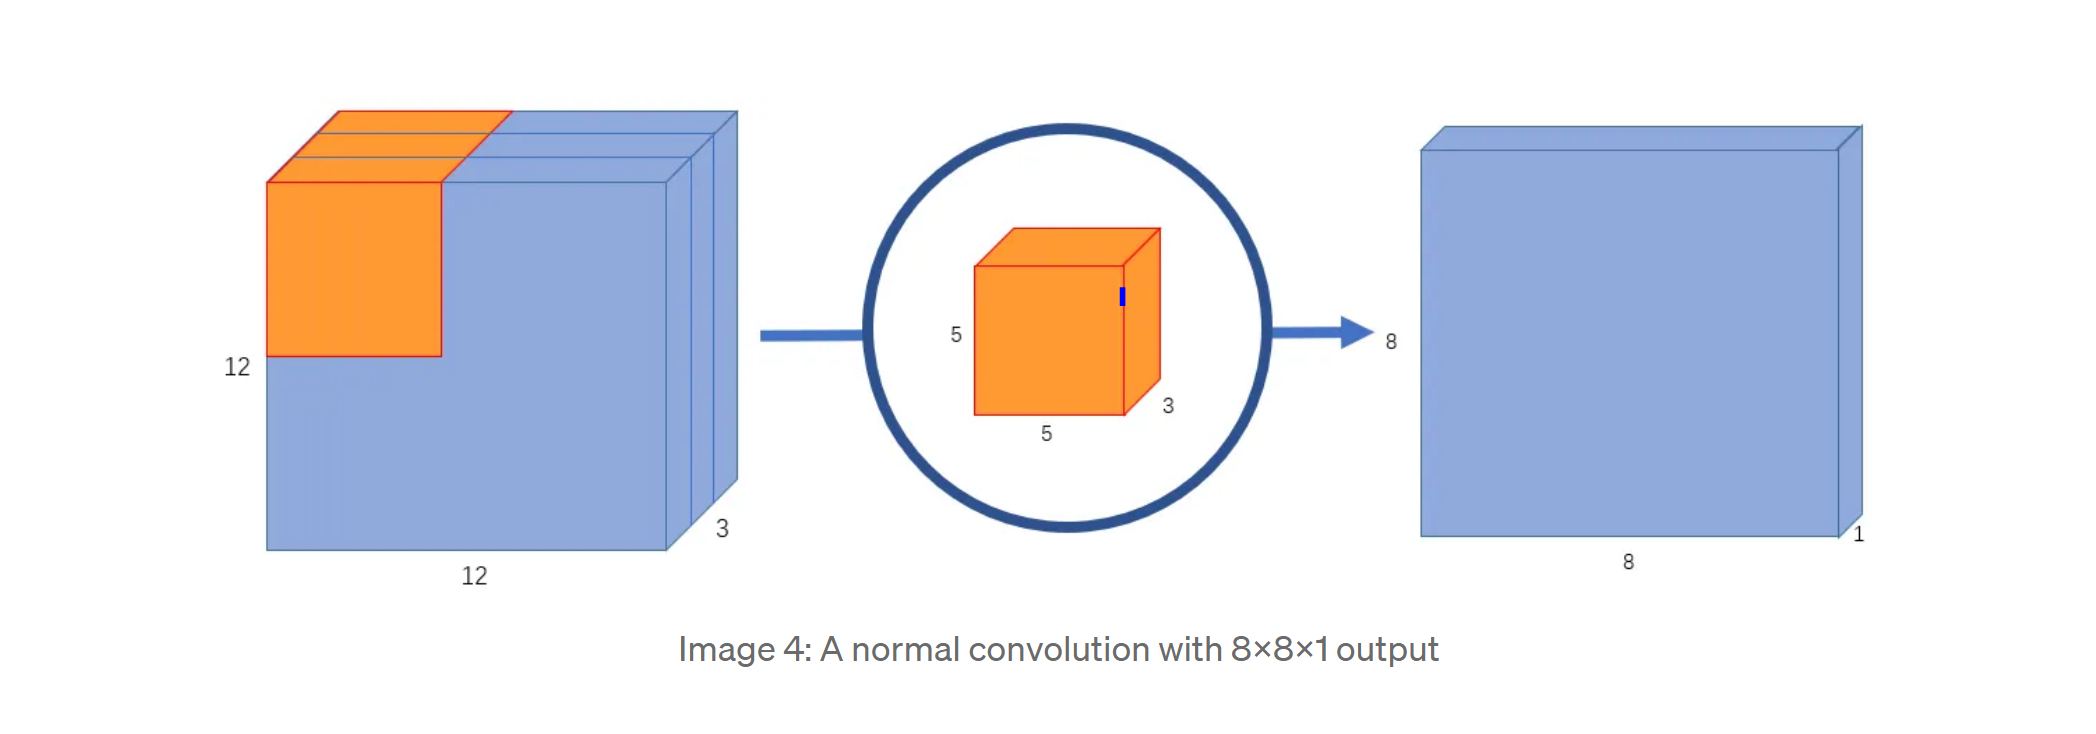
\includegraphics[width=0.8\textwidth]{./convolution.png} % Adjust the width as needed
\end{figure}

When we want to create many channels (e.g: 256 channels), we pass many (e.g: 256) kernels over the image: 
\begin{figure}[H]
    \centering
    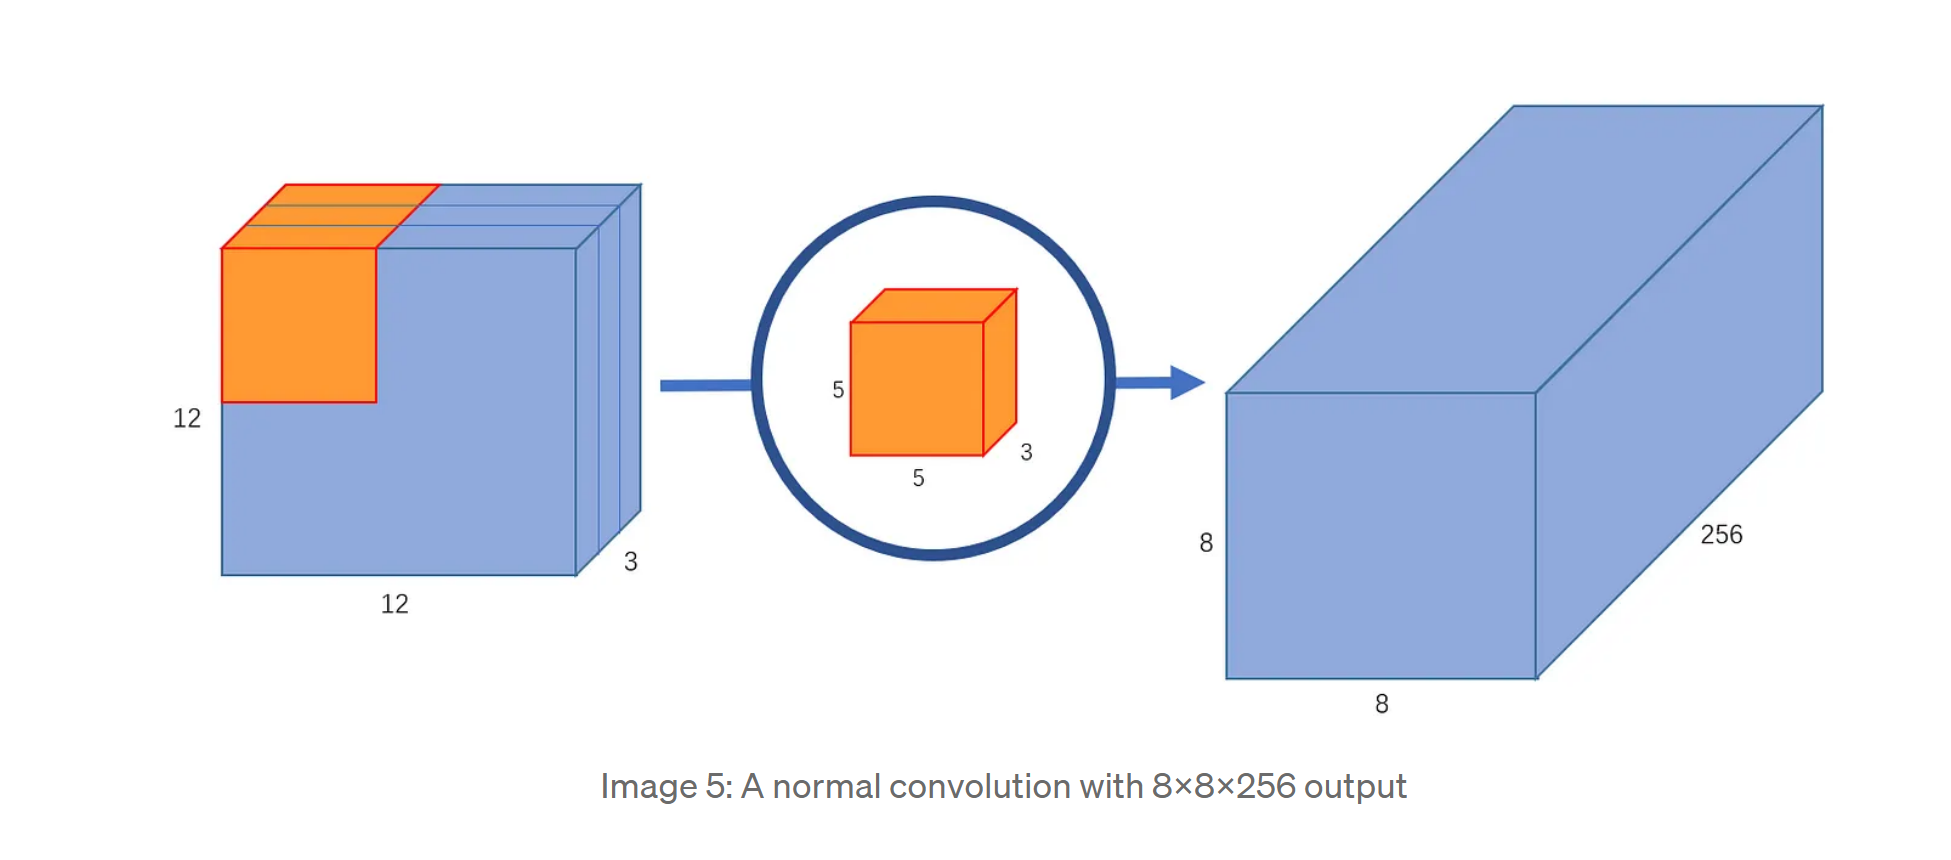
\includegraphics[width=0.8\textwidth]{./convolution_depth.png} % Adjust the width as needed
\end{figure}


\section{Depthwise Separable Convolution}
Depthwise Separable Convolution is the computational backbone used in MobileNet, a computer vision algorithm designed to do low latency object detection and classification at the edge. It differs from traditional convolution rather than passing \(N\) \(K \times K \times M\) filters across the image. We first pass \(M\) \(K \times K \times 1\) filters across the image, meaning we pass 1 kernel across each channel:

\begin{figure}[H]
    \centering
    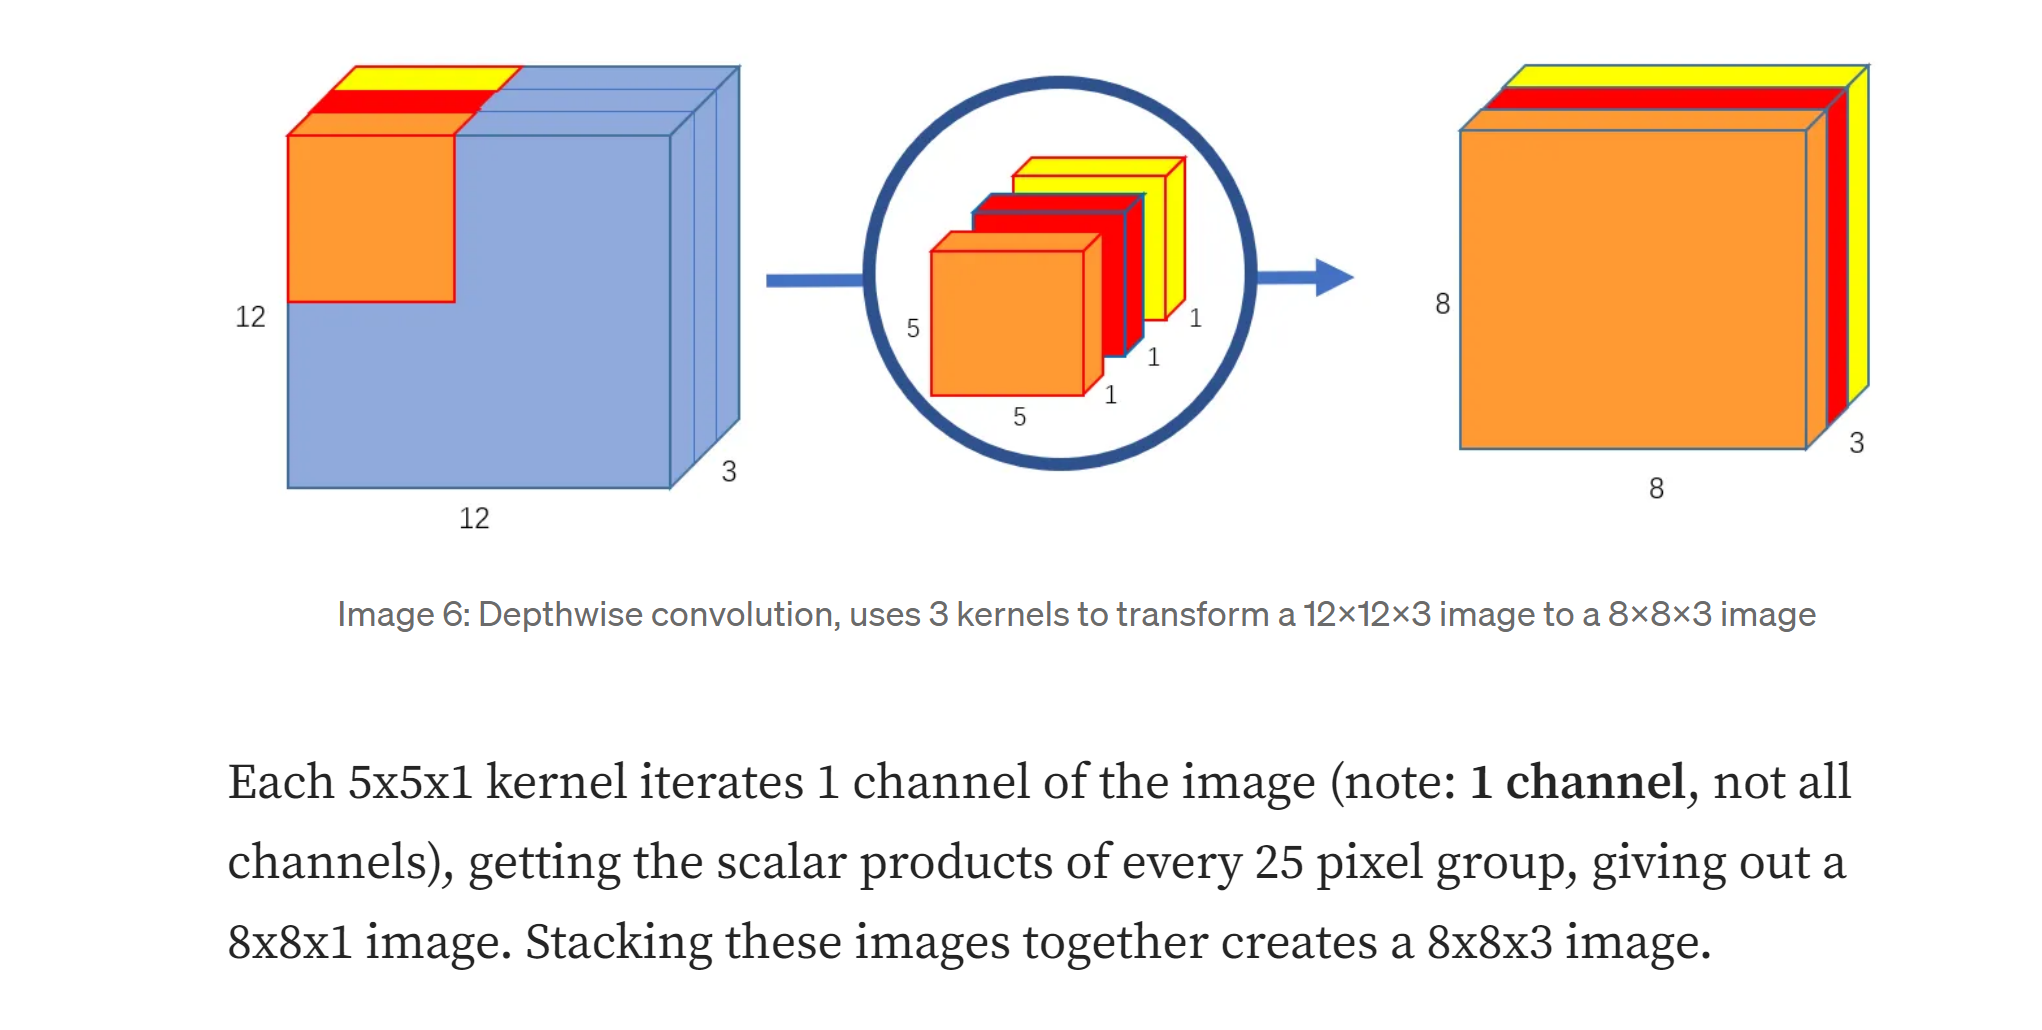
\includegraphics[width=0.8\textwidth]{./depthwise_1.png} % Adjust the width as needed

\end{figure}
Then, we create the desired depth dimension by passing \(N\) \(1\times 1\times M\) filters across the output from the first step. 


\begin{figure}[H]
    \centering
    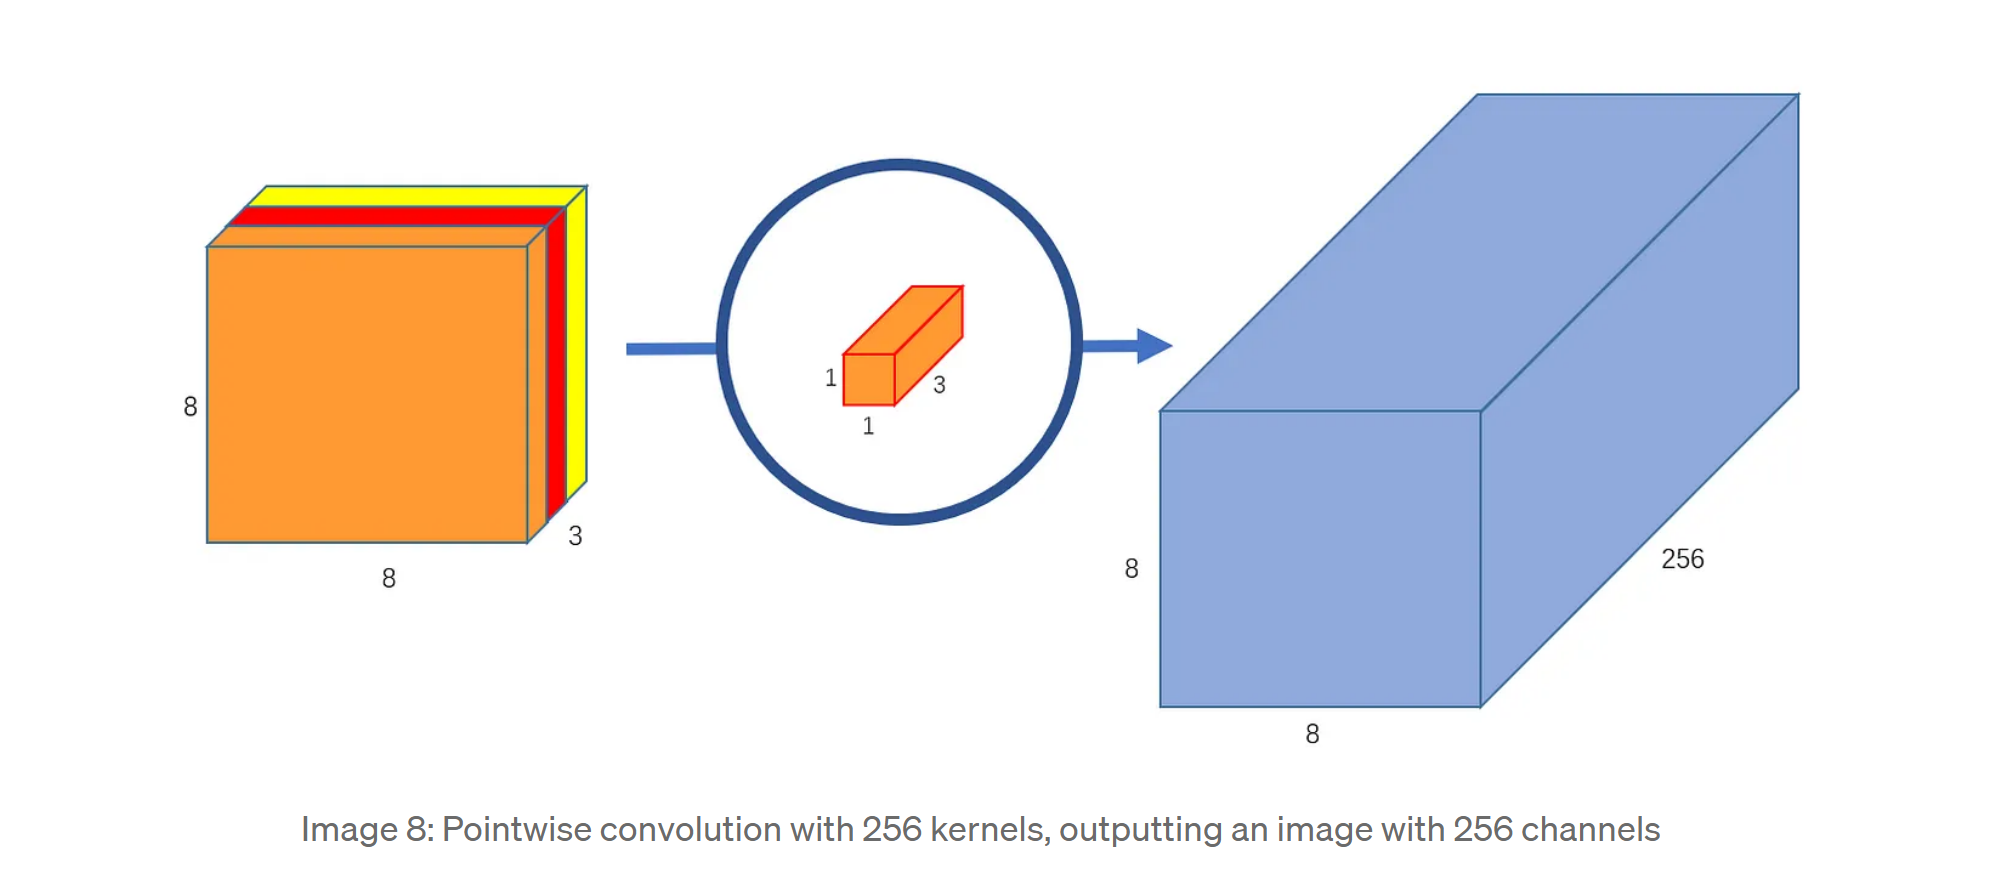
\includegraphics[width=0.8\textwidth]{./depthwise_2.png} % Adjust the width as needed
\end{figure}


This produces the same output shape as a traditional convolutional layer at a fraction of the computational cost. Why is this cheaper? In normal convolution, each layer will have

\[K \times K \times M \times C \times C \times N\]

Multiplications. This is because we have \(N\) total kernels. Each kernel will do \(C \times C\) total strides. And each stride involves \(K \times K \times M\) multiplications. \\

In contrast, depthwise separable convolution involves
\[(K \times K \times M) + (C \times C \times 1 \times 1 \times N)\]
Multiplications. This is a MUCH smaller number.

So it is more efficient. Another way of looking at this is that in traditional convolution we have (filling in with actual numbers) 256 \(5\times5\times3\) kernels, each of which moves \(8 \times 8\) times. In depthwise separable convolution, we have 256 \(1\times1\times3\) kernels each of which moves \(8 \times 8\) times, and then 3 \(5\times5\times3\) kernels which each move \(8 \times 8\)  times. You can see why this is more efficient. Obviously, it is also less accurate. But it can be immensely useful for edge deployed systems.

\section{K Nearest Neighbors}

K Nearest Neighbors (KNN) is a non-parametric, instance-based learning algorithm used for both classification and regression. By examining the 'k' closest data points in the feature space, KNN makes predictions based on the majority vote or average of these neighboring data points. (Instance based means a type of algorithm that makes predictions based on specific instances (or examples) from the training data, rather than deriving a generalizable model from the training data as in model-based learning).

\subsection{How it Works and Theoretical Foundations}

The KNN algorithm operates on a simple principle: similar things are near to each other. It predicts the label of a new point based on the labels of its closest neighbors. Here’s how it is implemented algorithmically and its underlying rationale:

\begin{itemize}
    \item \textbf{Distance Metric}: A metric, typically Euclidean distance, is used to calculate the closeness between points. For two points \(\mathbf{x}_i\) and \(\mathbf{x}_j\) in a \(d\)-dimensional space, the distance is defined as:
    \[
    d(\mathbf{x}_i, \mathbf{x}_j) = \sqrt{\sum_{k=1}^d (x_{ik} - x_{jk})^2}
    \]
    \item \textbf{Finding Nearest Neighbors}: For each query point, compute the distance to every point in the training set, then sort these points by distance. The top 'k' points are considered as the nearest neighbors.
    \item \textbf{Majority Voting or Averaging}: In classification, the predicted label is the most frequent label among the k nearest neighbors. In regression, it is the average of the values.
\end{itemize}

The effectiveness of KNN is fundamentally linked to the assumption that similar samples reside in close proximity, often referred to as the \textit{locality assumption}. This assumption is valid in many practical scenarios, especially when the feature space properly represents the underlying processes generating the data.

\subsection{Pros and Cons}

\textbf{When to Use KNN:}
\begin{itemize}
    \item For small to medium datasets where the curse of dimensionality is not a concern.
    \item In cases where model interpretability is important, as KNN's logic is straightforward and easy to explain.
    \item When a non-linear decision boundary is needed, as KNN can adapt to any shape of data distribution.
\end{itemize}

\textbf{Pros:}
\begin{itemize}
    \item No assumptions about the data distribution, making it versatile across different settings.
    \item Model updates are inexpensive—new data can be added without significant computational costs.
    \item Simple to implement and understand.
\end{itemize}

\textbf{Cons:}
\begin{itemize}
    \item Sensitive to the local structure of the data, which can be a disadvantage with noisy data.
    \item Computationally expensive as the dataset grows, due to the need to compute distances for each query.
    \item Performance degrades with high dimensionality unless dimension reduction techniques are applied.
\end{itemize}

K Nearest Neighbors is a robust algorithm for problems where the decision boundary is irregular, making it a powerful tool for both classification and regression tasks in scenarios where the inherent data structure is well represented by the feature space.


\section{Fisher's Linear Discriminant Ratio}


Fisher's Linear Discriminant Ratio, often simply referred to as Fisher's Linear Discriminant, is a dimensionality reduction technique that involves projecting our data into a lower dimensional feature space that maximizes the ratio of between-class scatter to in-class scatter:

\[ J(w) = \frac{\sigma_{\text{between}}^2}{\sigma_{\text{within}}^2} = \frac{w^T S_B w}{w^T S_W w} \] 

This ensures maximum linear separability by maximizing the distance between the means of the classes, while minimizing the variability of the data inside the class itself. In some ways, it can be thought of as a signal-to-noise ratio (pretty cool connection that provides intuition for why this is useful). Here, \( S_W \) is the within-class scatter matrix: 

\[ S_W = \sum_{i=1}^{c} \sum_{x \in X_i} (x - \mu_i)(x - \mu_i)^T \]

Where \( X_i \) is the set of samples for class \( i \) and \( \mu_i \) is the mean of samples for class \( i \). \( S_B \) is the between-class scatter matrix for two classes with means \( \mu_1 \) and \( \mu_2 \)

\[S_B = \sum_{i=1}^{c} N_i (\boldsymbol{\mu}_i - \boldsymbol{\mu})(\boldsymbol{\mu}_i - \boldsymbol{\mu})^T\]

Where \(c\) is the number of classes, \(N_i\) is the number of samples in class \(i\), \(mu_i\) is the within-class mean vector for class \(i\), and \(mu\) is the overall mean vector for the entire dataset. Note that \(\mu_i\) and \(x\) are both d-dimensional vectors where d is the number of features in our dataset:

\[S_B, S_W \in (\mathbb{R}^d \times \mathbb{R}^d)\]

It's worth noting that the discriminants found via FLD are NOT decision boundaries themselves. They are a new direction into which we project the data. For example, if we are doing binary classification the discriminant would be a hyperplane in d-dimensions that we multiply our dataset by. The result will be the same dataset in a 1-dimensional feature space (so just a number line). The decision boundary in this space would be a single scalar value we use as a threshold. This is not the same as a the discriminator (whch again is a d-length vector).

\subsection{How it works}

We need find \(w\), the matrix comprised of \(c-1\) column vectors representing the directions that maximize the FLDR. To find this, we need to solve

\[S_w^{-1}S_bw = \lambda w\]

This should look familiar. This is just eigendecomposition. Once we've solved this, we'll have up to \(c-1\) discriminants between our classes. We then project our data into this newer, lower dimensional feature space by doing

\[X_{new} = XW\]

And hopefully then we have data that is more easily separable. 

\(\textbf{Why is this projecting it into a lower dimension?}\): \\This is the size of all the different matrices involved: 

\[(n \times k) = (n \times d) \cdot (d \times k) \{k \in 1...c-1\}\]

Also, even if we have a weird example where the number of classes \(c\) is greater than the number of features \(d\), it is not possible for the dimension of our data to increase or stay the same. this is because it is not possible to have more linearly independent vectors (\(k\)) than the dimension of our feature space. So in reality:
\[k \in 1...min(c-1, d)\]

\(\textbf{Why do we have a maximum of \(c-1\) discriminants?}\):\\ A matrix of size \((d \times d)\) and rank \(c\) will have \(c\) linearly independent eigenvectors. The rank of a matrix is the dimension of the vector space spanned by its columns. In other words, the rank of the matrix is the number of linearly independent columns in the matrix. A matrix of rank \(c\) will have \(c\) nonzero eigenvalues and \(c\) linearly independent eigenvectors. \(S_B\) is of rank \(c\) because in 

\[S_B = \sum_{i=1}^{c} N_i (\boldsymbol{\mu}_i - \boldsymbol{\mu})(\boldsymbol{\mu}_i - \boldsymbol{\mu})^T\]

The matrix \((\boldsymbol{\mu}_i - \boldsymbol{\mu})(\boldsymbol{\mu}_i - \boldsymbol{\mu})^T\) is the outer product of the matrix \((\boldsymbol{\mu}_i - \boldsymbol{\mu})\) with itself. And the rank of the outer product of any matrix with itself is 1.

\subsection{When to Use Fisher's Linear Discriminant Ratio vs. PCA}

FLD is better to use when we are doing classification and want to enhance predictive accuracy. PCA is a more general dimensionality reduction technique which just seeks to preserve as much of the information present as possible without heed to separability.

\subsection{How is this different from PCA?}
Both FLD and PCA reduce dimensionality, but they do so with different goals. PCA seeks directions that maximize variance without consideration of class labels, while FLD seeks directions that are good at separating classes. Mathematically, both involve eigendecomposition. In PCA we do eigendecomposition directly on the covariance matrix (meaning we care aobut preserving the variance between features, rather than classese), while in FLD we do eigendecompostion on a matrix representing the ratio of between class scatter to in-class scatter (meaning we care about preserving  the variance between classes, rather than features)

\textbf{Use FLD when}:
\begin{itemize}
    \item Effective in cases where features are normally distributed and have similar covariance matrices (i.e the features vary similarly between classes).
    \item We're doing classification and want to enhance predictive accuracy of the classifier we eventually build
\end{itemize}

\textbf{Don't use FLD when}:
\begin{itemize}
    \item Classes aren't normally distributed or the covariance matrices aren't similar (use PCA here).
    \item Not suitable for non-linear class distributions.
\end{itemize}

\subsection{The Deep, Bayesian Decision Theory Justification for FLD}

If we assume the data for each class are generated from a multivariate Gaussian distribution, the likelihood of observing the data \(x\) given it is in class \(y=i\) is given by:

\[P(x | y = i) = \frac{1}{(2\pi)^{d/2}|\Sigma_i|^{1/2}}e^{(-\frac{1}{2})(x - \mu_i)^T\sigma_i^{-1}(x - \mu_i)}\]

In the two class problem (this is more complicated otherwise, but still holds), we can design a Maximum Likelihood Ratio by setting a threshold value \(\gamma = 1\) based on a sufficient statistic, which is calculated by solving for the log likelihood ratio:

\[\ln(\gamma) = 0 = \ln\left(\frac{|\Sigma_2|^{1/2}e^{-\frac{1}{2}(x - \mu_1)^T\sigma_1^{-1}(x - \mu_1)}}{|\Sigma_1|^{1/2}e^{-\frac{1}{2}(x - \mu_2)^T\sigma_2^{-1}(x - \mu_2)}}\right)\]

If we assume \(\Sigma_1 \approx \Sigma_2 \approx \Sigma\) (note why this assumption is so important! Without it nothing cancels), we get:

\[x^T\Sigma^{-1}(\mu_1 - \mu_2) - \frac{1}{2}(\mu_1^T\Sigma^{-1}\mu_1 - \mu_2^T\Sigma^{-1}\mu_2)\]

This means that \(x^T\Sigma^{-1}(\mu_1 - \mu_2)\) is our sufficient statistic (because the 2nd part of the equation is constant). Now, if we look at our equation for J(w), we see that we want to maximize

\[S_B = w^T(\mu_1 - \mu_2)(\mu_1 - \mu_2)^Tw\]

This aligns with our sufficient statistic, meaning that we can guarantee maximum separation if we choose \(w\) such that:

\[w \propto \Sigma^{-1}(\mu_1 - \mu_2)\]

This is the deep justification from bayesian estimatino theory for why FLD works. But it also means that \(w\) must fit the same constrains we need for MLE (at least approximately) or it will not perform well. 



% Include the figure
\begin{figure}[H]
    \centering
    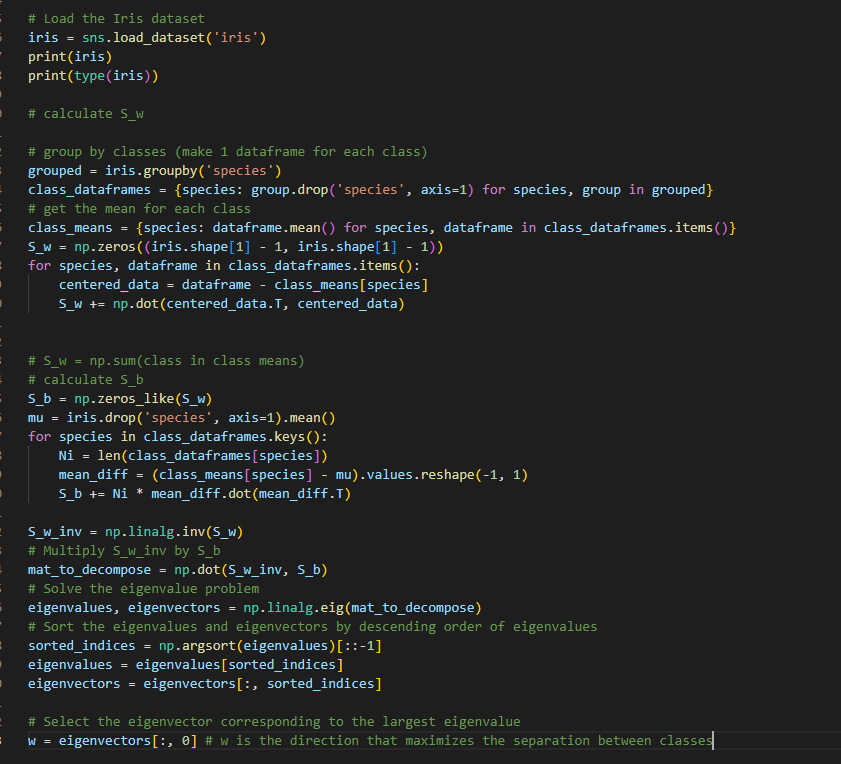
\includegraphics[width=0.8\textwidth]{./FLD_calculation.png} % Adjust the width as needed
    \caption{Python Code for computing Fischer's Linear Discriminant. Note, if you want k discriminants, replace w[:,0] with w[:,:k]}
\end{figure}
\section{Oversampling}
Oversampling refers to a set of techniques used in machine learning to reduce class imbalances by either bootstrap sampling from underrepresented classes or interpolating between existing samples of underrepresented classes with the intent of producing some new, less imbalanced dataset. Here I briefly introduce two methods:

\subsection{Random Oversampling}
Random oversampling duplicates samples from the minority class until it achieves some desired balance within the majority class. Let's say we have some dataset \(D = \{x_i, y_i\}_{i=1}^N\). And let \(D_\text{min}\) and \(D_\text{maj}\) represent subsets representing all data points belonging to the majority class and some minority class. Let's say the number of samples \((x_i, y_i) \in D_\text{min}\) is \(N_\text{min}\) and the number of samples \((x_i, y_i) \in D_\text{maj}\) is \(N_\text{maj}\). Because  \(D_\text{min}\) is a minority class \(N_\text{min} << N_\text{maj}\). We random sample with replacement from \(D_\text{min}\) to produce \(k\) additional samples, which are then appended to the new dataset:
\[D_\text{new} = D \cup \{(x_i, y_i) | (x_i, y_i) \in D_\text{min}, i=1, \ldots, k\}\]

This has the limitation that it can lead to overfitting because it repeats exact samples from the minority class, without creating new information or diversity in the dataset.

\subsection{Synthetic Minority Over-sampling Technique (SMOTE)}
SMOTE creates synthetic examples from the minority class \(D_\text{min}\)  by interpolating between existing minority class samples. This introduces more diversity into the minority class while maintaining its feature distribution. Here's the mathematical formulation of hte technique:\\

\begin{enumerate}
\item Select a sample \((x_i, y_i) \in D_\text{min}\) and one of its \(k\) nearest neighbors \((x_j, y_j)\) (randomly chosen)
\item Generate a new synthetic sample \(x_\text{new}, y_i\) as:
\[x_\text{new} = x_i + \lambda(x_j - x_i), \lambda \sim U(0,1)\]
This creates a new sample that is sampled uniformly and at random between \(x_i\) and \(x_j\). 
\item Then do this however many times you want, and concatenate the results iwth the original dataset as shown above
\end{enumerate}
This technique obviously may not hold for things like image data that are not \emph{space-linear}. But for tabular data it's often good. 

\subsection{Generative Methods}
There are methods involving training various generative models (GANs, VAEs, LLMs, Diffusion Models) to produce synthetic data. These are best understood by learning about the aforementioned models themselves. in all cases,  you train a generative model to produce the desired synthetic data, then you use that synthetic data in your augmented dataset.

\section{F1 Score and F2 Score}

The F1 score is a harmonic mean of precision and recall, providing a balance between them. It is particularly used when there is a need to find a balance between precision and recall. The F2 score, on the other hand, weighs recall higher than precision, beneficial in situations where missing a positive instance is costlier than incorrectly labeling a negative instance as positive.

\subsection{F1 Score}

\textbf{Definition:} The F1 score is the harmonic mean of precision and recall, offering a balance between the two by penalizing extreme values. It is defined as:

\textbf{Mathematical Formula:}
\[ F1 = 2 \cdot \frac{\text{Precision} \cdot \text{Recall}}{\text{Precision} + \text{Recall}} \]

where Precision is the ratio of true positive results to the total number of positive results predicted, and Recall is the ratio of true positive results to the total number of actual positive instances.

\subsection{F2 Score}

\textbf{Definition:} The F2 score modifies the F1 score to weigh recall more than precision, using a factor of 2 to square the importance of recall. It is defined as:

\textbf{Mathematical Formula:}
\[ F2 = 5 \cdot \frac{\text{Precision} \cdot \text{Recall}}{4\cdot\text{Precision} + \text{Recall}} \]

This formula arises from the general formula for the F-score:
\[ F_\beta = (1 + \beta^2) \cdot \frac{\text{Precision} \cdot \text{Recall}}{\beta^2 \cdot \text{Precision} + \text{Recall}} \]
where \( \beta \) is chosen based on the desired emphasis on precision versus recall. For the F2 score, \( \beta = 2 \).

\textbf{How does F2 score weight recall more given that we're multiplying precision by \( \beta \)?}

Because if precision remains high but recall is low the beta value in the denominator will be higher, and thus the overall F2 score will be lower. but if we have the reverse (low precision, high recall), then the f2 score will be higher because the numerator will remain the same but the denominator is lower in this scenario. For example, 

\[ F2 = \frac{5 \cdot P \cdot R}{4P + R} \]

\textbf{Scenario A} (High Precision, Lower Recall):
\begin{itemize}
    \item Precision (\(P\)) = 0.9
    \item Recall (\(R\)) = 0.5
\end{itemize}

The F2 score calculation for Scenario A is:
\[ F2_A = \frac{5 \cdot 0.9 \cdot 0.5}{4 \cdot 0.9 + 0.5} \approx 0.549 \]

\textbf{Scenario B} (Lower Precision, High Recall):
\begin{itemize}
    \item Precision (\(P\)) = 0.5
    \item Recall (\(R\)) = 0.9
\end{itemize}
The F2 score calculation for Scenario B is:
\[ F2_B = \frac{5 \cdot 0.5 \cdot 0.9}{4 \cdot 0.5 + 0.9} \approx 0.776 \]
\subsection{Usage Guidelines}

\textbf{When to Use F1 Score:}
\begin{itemize}
    \item In scenarios where false positives and false negatives are equally costly.
    \item When there is a need for a single metric to compare models' performance directly.
\end{itemize}

\textbf{When to Use F2 Score:}
\begin{itemize}
    \item In situations where we care more about missing positive instances (false negatives) having too many false positives. 
    \item Ideal for applications like medical diagnosis or fraud detection, where failing to detect true positives can have serious consequences.
\end{itemize}

\textbf{When Not to Use:}
\begin{itemize}
    \item These scores should not be used in isolation when the cost of false positives and false negatives varies widely across different contexts.
    \item Not suitable for datasets with highly imbalanced classes without adjusting the model's decision threshold or considering other metrics like ROC-AUC.
\end{itemize}
\section{GeLU \& ReLU}
ReLU (Rectified Linear Unit) and GeLU (Gaussian Error Linear Unit) are two very common and very similar activation functions used in deep neural networks and transformers. \\
\subsection{ReLU}

ReLU is very simple: 

\[
\text{ReLU}(x) = \max(0, x)
\]

It acts as a linear filter, only activating signals from the linear layer preceding it if they are greater than 0. ReLU's gradient is:

\[
\text{ReLU}'(x) = 
\begin{cases} 
      1, & \text{if } x > 0 \\
      0, & \text{if } x \leq 0 
   \end{cases}
\]
\[
\text{ReLU}(x) = \max(0, x)
\]

It acts as a linear filter, only activating signals from the linear layer preceding it if they are greater than 0. ReLU's gradient is:

\[
\text{ReLU}'(x) = 
\begin{cases} 
      1, & \text{if } x > 0 \\
      0, & \text{if } x \leq 0 
   \end{cases}
\]

This makes it useful in deep neural networks because it clearly propagates a reward signal back to the weights which produced it, allowing for credit assignment to occur without gradients exploding or vanishing.\\
\textbf{Dead Neuron Problem}: The dead neuron problem happens when a neuron outputs a negative value and, due to ReLU's nature of zeroing out negative actions, has a gradient of 0. As a result, the neuron's weights may never update, effectively "killing" the neuron. \\

It's not as cut-and-dry as this in reality because if inputs are properly normalized, most of the time, there are few neurons for which the output will always be negative. But this does happen. \\ 

To fix this, LeakyReLU was developed, which has a slightly positive slope (nonzero gradient) for negative values: 


\begin{figure}[H]
    \centering
    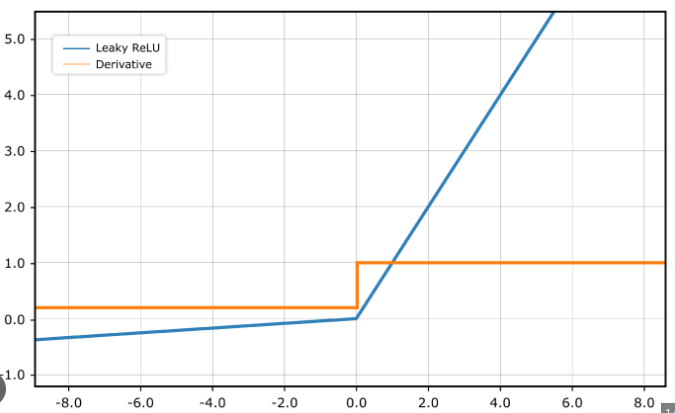
\includegraphics[width=0.8\textwidth]{LeakyReLU.png} % Adjust the width as needed
\end{figure}

\textbf{ReLU and Batchnorm}: If ReLU only allows positive signals through, why doesn't this prevent the neural net from expressing negative numbers? Because BatchNorm exists. Using ReLU without batchnorm results in a neural net that suffers from this exact problem and will not learn.

\subsection{GeLU}
The formula for GeLU is: 

\[\text{GeLU}(x) = x \cdot \phi(x)\]

Where \(\phi(x)\) is the gaussian CDF for the standard normal distribution \(\mu_x=0, \text{var}(x)=1)\):

\[\phi(x) = \frac{1}{2}\left(1 + \text{erf}(\frac{x}{\sqrt{2}})\right)\]

\[\text{erf}(x) =\frac{2}{\sqrt{\pi}} \int_0^xe^{t^2}dt\]


GeLU is a more expressive version of ReLU. ReLU filters out low-importance signal using the simple decision rule \(x>0\). GeLU dynamically and smoothly performs this filtering by multiplying each output \(x\) by its CDF value. for large x, \(\phi(x) \sim 1\), while for smaller x \(\phi(x) \sim 0\). This provides a more nuanced and expressive activation that is useful for transformers and networks where sparsity is less important. \\

Here are two things GeLU solves that ReLU Does not: 
\begin{enumerate}
\item \textbf{GeLU also solves the dead neuron problem}: The gradient of GeLU is 
\[
\frac{d}{dx} \text{GeLU}(x) = \Phi(x) + x \cdot \phi(x)
\]

where \(\Phi(x)\) is the standard normal Gaussian CDF and \(\phi(x)\) is its derivative, the standard normal Gaussian PDF
\[
\Phi(x) = 0.5 \left( 1 + \text{erf}\left(\frac{x}{\sqrt{2}}\right) \right)
\]
and
\[
\phi(x) = \frac{1}{\sqrt{2 \pi}} e^{-\frac{x^2}{2}}
\]

\(\phi(x)\) is obviously is obviously nonzero for all \(x\)
\item \textbf{GeLU creates a separation effect for significant and insignificant neurons, while preventing unbounded growth in weight values}: This might be harder to understand, but it's very important. \\

\textbf{For Positive x}: GeLUs gradient is positive, but approaches 0 as inputs become large. This soft cap creates a leveling off effect while ensuring significant neurons are weighted more highly. \\

\textbf{For Negative x}: GeLUs gradient is also positive, meaning weights associated with negative x will decrease further, while still approaching 0 for highly negative values. \\

\begin{figure}[H]
    \centering
    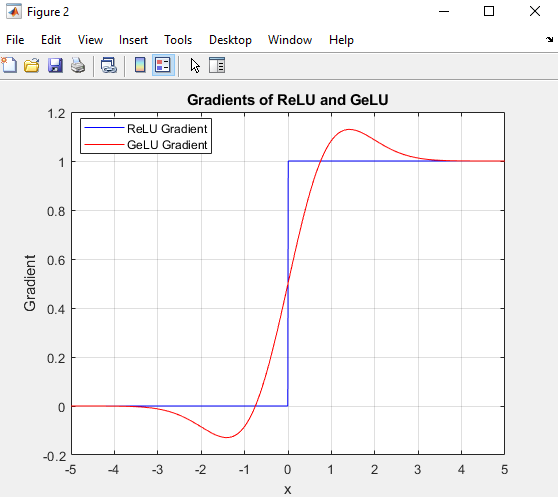
\includegraphics[width=0.7\textwidth]{relugelu.png} % Adjust the width as needed
\end{figure}
Taken together, this means the gradient pushes significant and insignificant signals apart.  
\end{enumerate}
\textbf{Notes}:
\begin{itemize}
\item ReLU is better when sparsity in the output signals is important
\item ReLU is computationally much cheaper than GeLU
\item Layer Normalization in Transformers prevents GeLU from having vanishing / exploding gradients. 
\end{itemize}
\section{Transformers}
Transformers are a class of deep learning models that primarily use self-attention mechanisms to process sequences of data without relying on recurrence (unlike LSTM's and RNN's), making them highly parallelizable and efficient. 'Attention' is a mechanism that allows models to dynamically focus on different parts of the input data by weighting each token of the data according to its relevance and significance, and directly modeling the relationships between elements in the input sequence regardless of their positional distance. Attention mimics the human ability to focus more on certain stimuli than others, depending on the task at hand. These some advantages Transformers have over earlier machine learning architectures: 

This diagram details the steps by which information is processed in a transformer. Here I explain each part thoroughly.

\begin{figure}[H]
    \centering
    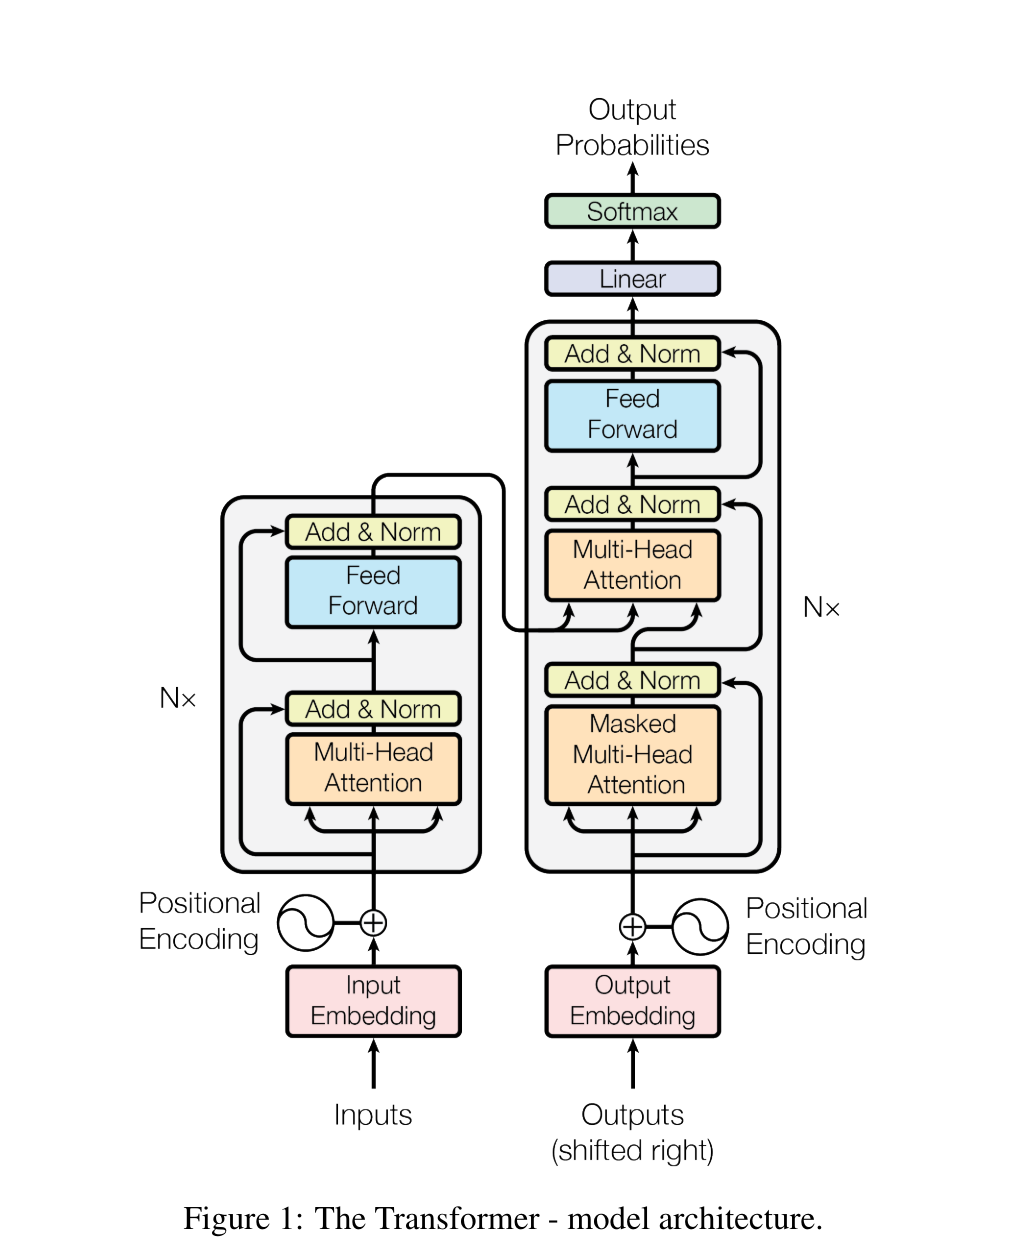
\includegraphics[width=0.8\textwidth]{./Transformer_Architecture.png} % Adjust the width as needed
    \caption{This figure shows the components of a transfomer.}
    \label{fig:gaussian_kde}
\end{figure}

\begin{enumerate}
\item \textbf{Input Embedding}: 
First, each word (token) is converted into a vector. The vectors for every word in our vocab are placed intoa large lookup table, which is referenced by the algorithm. The idea is that the semantic relationship between words is captured by their spatial orientation in the high-dimensional vector space they have been embedded in: 

\[sim \langle u, v \rangle = \frac{u \cdot v }{||u|| ||v||}\]

Also, the spatial relationship of the vectors capture more intricate relationships between words: Word2Vec(king) \(-\) Word2Vec(man) = Word2Vec(queen), for example. The embedding algorithm is a neural network and can either be pre-trained (so just the embeddings are imported) or can be a learned alongside the transformer. Many embedding algorithms rely on principles from linguistics such as distributional semantics (you shall know a word by the company it keeps) to create this spatial distribution.

\item \textbf{Positional Encoding} Next, a vector of equal length to the embedding is added to each token. Each vector encapsulates the relative positions of its token within a target sequence. The positional encodings provide the transformer model with information about where the words are in the input sequence. The function guarantees that each token will have a unique positional encoding: 

\[
\text{PE}(\text{pos}, i) = 
\begin{cases} 
\sin\left(\frac{\text{pos}}{10000^{2i/d}}\right) & \text{if } i \text{ is even} \\
\cos\left(\frac{\text{pos}}{10000^{2i/d}}\right) & \text{if } i \text{ is odd}
\end{cases}
\]
where \(\text{pos}\) is the position of the token in the sequence. \(\text{Pos}=0\) means this is the \(0^{th}\) token in our sample. i is the dimension.  \(\text{i}=0\) means we're looknig at the \(0^{th}\) entry in the vector embedding for tokens[pos]. d is the total length of the embedding vector. 
Notice that the period and phase of each pair of sinusoids will be unique (See picture below). This is why each positional encoding is unique. \\

Each token's positional encoding is added to the input embedding for that token and then passed to the first multiheaded attention module.


\begin{figure}[H]
    \centering
    \includegraphics[width=0.8\textwidth]{./Positional_Encoding.png} % Adjust the Poidth as needed
    \caption{A visualization of the positional encoding vectors in a transformer. Position denotes the \(i^{th}\) word in a sequence and vector index denotes the \(i^{th}\) entry in the embedding for the \(j^{th}\) word. So here our transformer can handle up to 1000 inputs and embeds each token into 60 dimensions.}
\end{figure}

Here is code for a positional embedding function in a transformer. Note that this is not parallelized so it can be understood more intuitively. 


\begin{figure}[H]
    \centering
    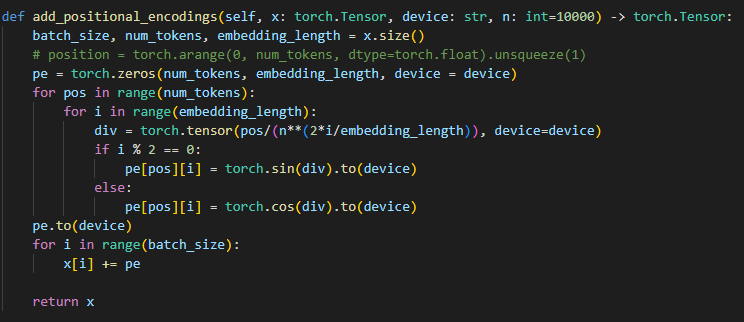
\includegraphics[width=0.8\textwidth]{./Positional_encoding_python_function.png} % Adjust the Poidth as needed
\end{figure}

\item \textbf{Linear Transformations}: The formula for self-attention is: 
\[Z = \text{Softmax}(\frac{Q K^T}{\sqrt{d_k}})\cdot V\]

Where Q, K, and V are the Query, Key, and Value matrices respectively. Before we do attention, we need to create these matrices. We start with our input matrix \(Z\):
\begin{figure}[H]
    \centering
    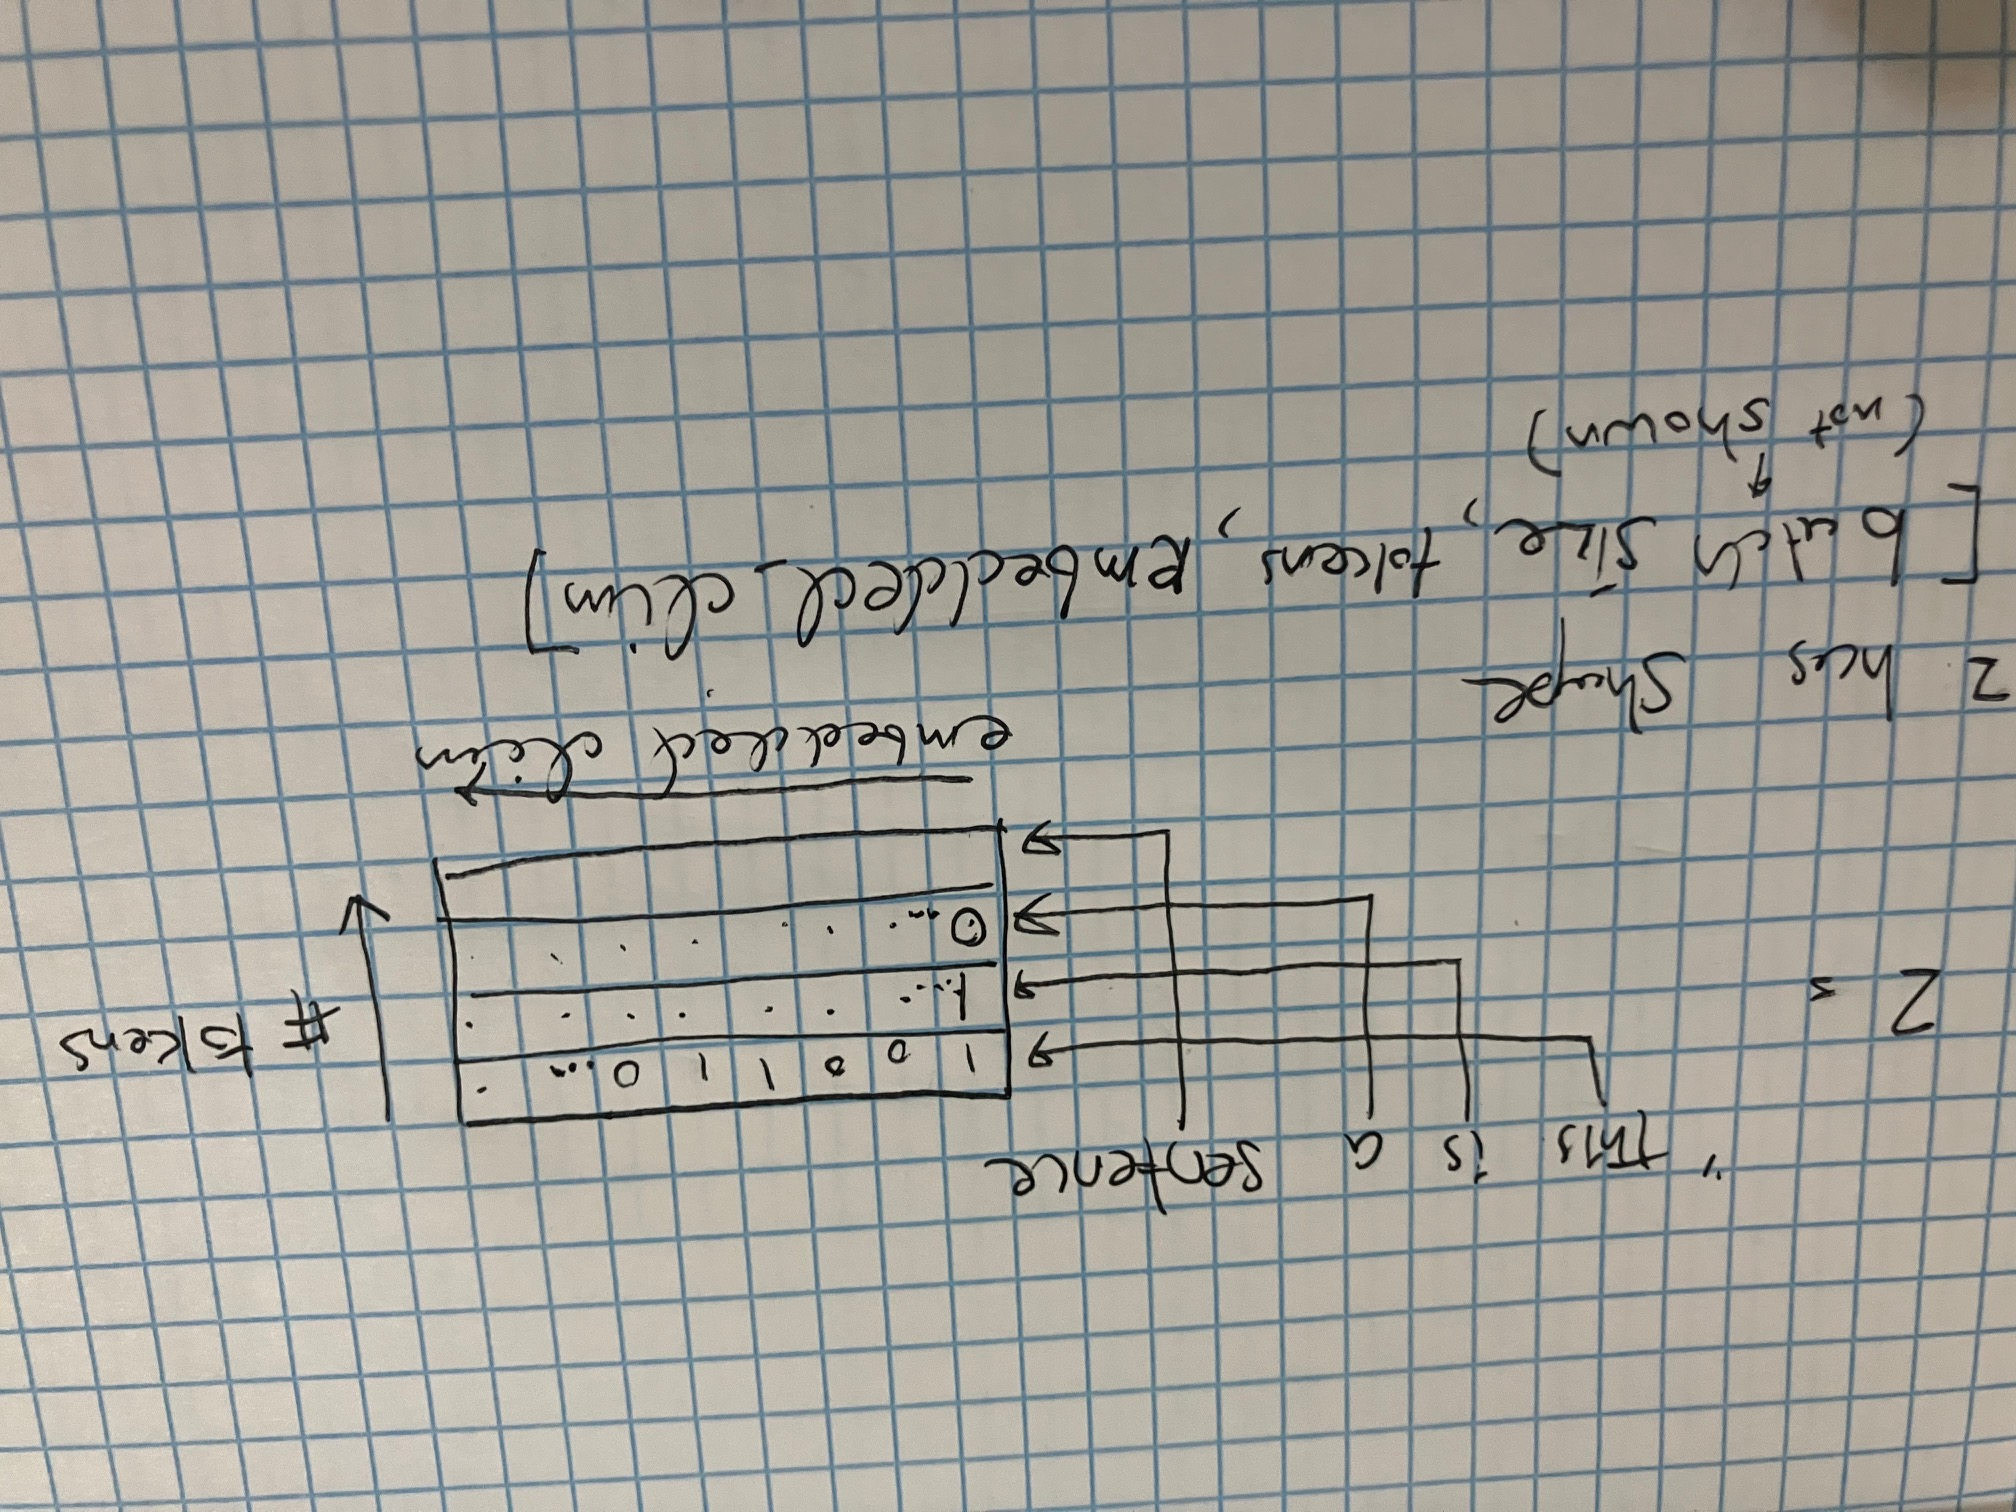
\includegraphics[width=0.8\textwidth, angle=180]{./linear_transformation.jpg}
\end{figure}
I have shown the first layer here, where Z is literally just the vector embeddings plus the positional embeddings concatenated togehter. In subsequent layers, \(Z\) will be the output from the previous layer. But its shape will be the same as here:

\[Z = [\text{batch\_size, num\_tokens, embedded\_dims}]\]

The embedded dims is the original length of the embedding vectors (the dimensionality of the vector space).\\

Now, we take three copies of Z and matrix multiply each by the learnable weights \(W_q, W_k, W_v\):


\[Q= ZW_Q\]
\[K = ZW_K\]
\[V_i = ZW_V\]

\begin{figure}[H]
    \centering
    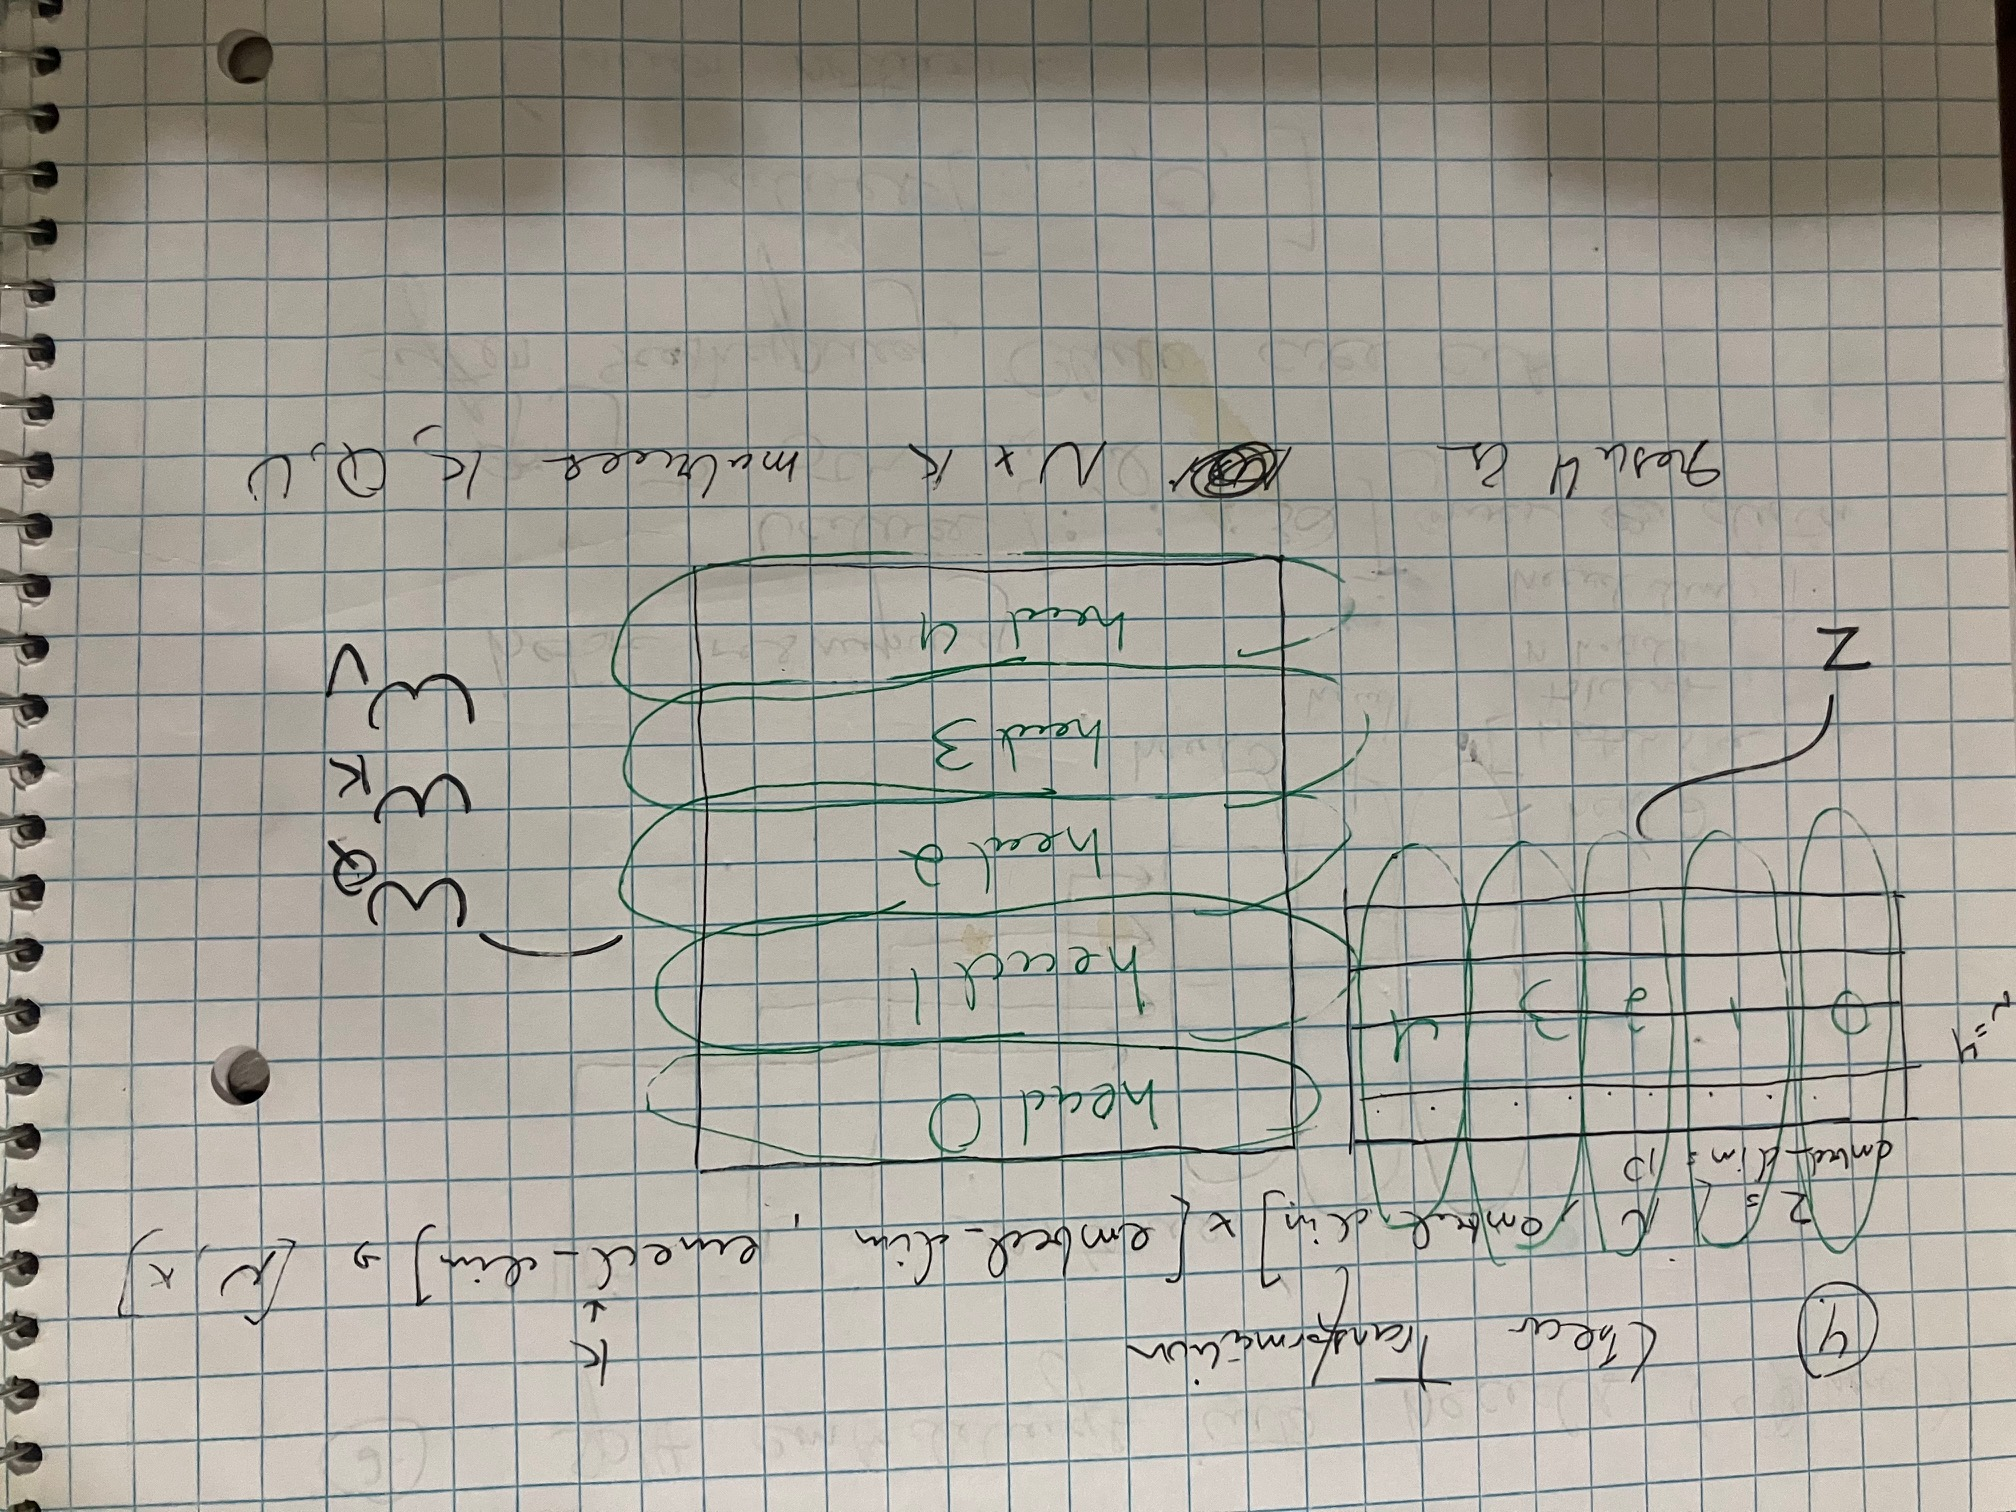
\includegraphics[width=0.8\textwidth, angle=180]{./linear_2.jpg}
\end{figure}

It's worth noting that this operation can be done before or after splitting into heads. As shown above it is done before. In this case the dimensions of the matrices invovled are:

\begin{align*}
[\text{batch\_size, num\_tokens, embedded\_dims}] \times [\text{embedded\_dims, d\_ff}] \\
\rightarrow [\text{batch\_size, num\_tokens, d\_ff}]
\end{align*}
d\_ff represents the latent space, a higher-dimensional embedding space the inputs are projected into before self-attention. This is not always done and it is quite common to also set d\_ff equal to embedding\_dims. Also, note that the weights for the heads are all in one common matrix \(W_Q, W_K, W_V\), and each head occupies a certain number of rows in this matrix.\\

Note that if we split into heads first before doing our linear transformations, each will have shape

\[\text{[batch\_size, head\_dim, d\_ff]}\]

Where \(\text{head\_dim} \times \text{n\_heads} = \text{embedded\_dims}\). This means that in this case our overall matrix multiplication looks like this: 

\begin{align*}
[[\text{batch\_size, num\_tokens, n\_heads, head\_dim}] \times \text{batch\_size, num\_tokens, n\_heads, d\_ff}] \\
\rightarrow [\text{batch\_size, num\_tokens, d\_ff}]
\end{align*}
\begin{figure}[H]
    \centering
    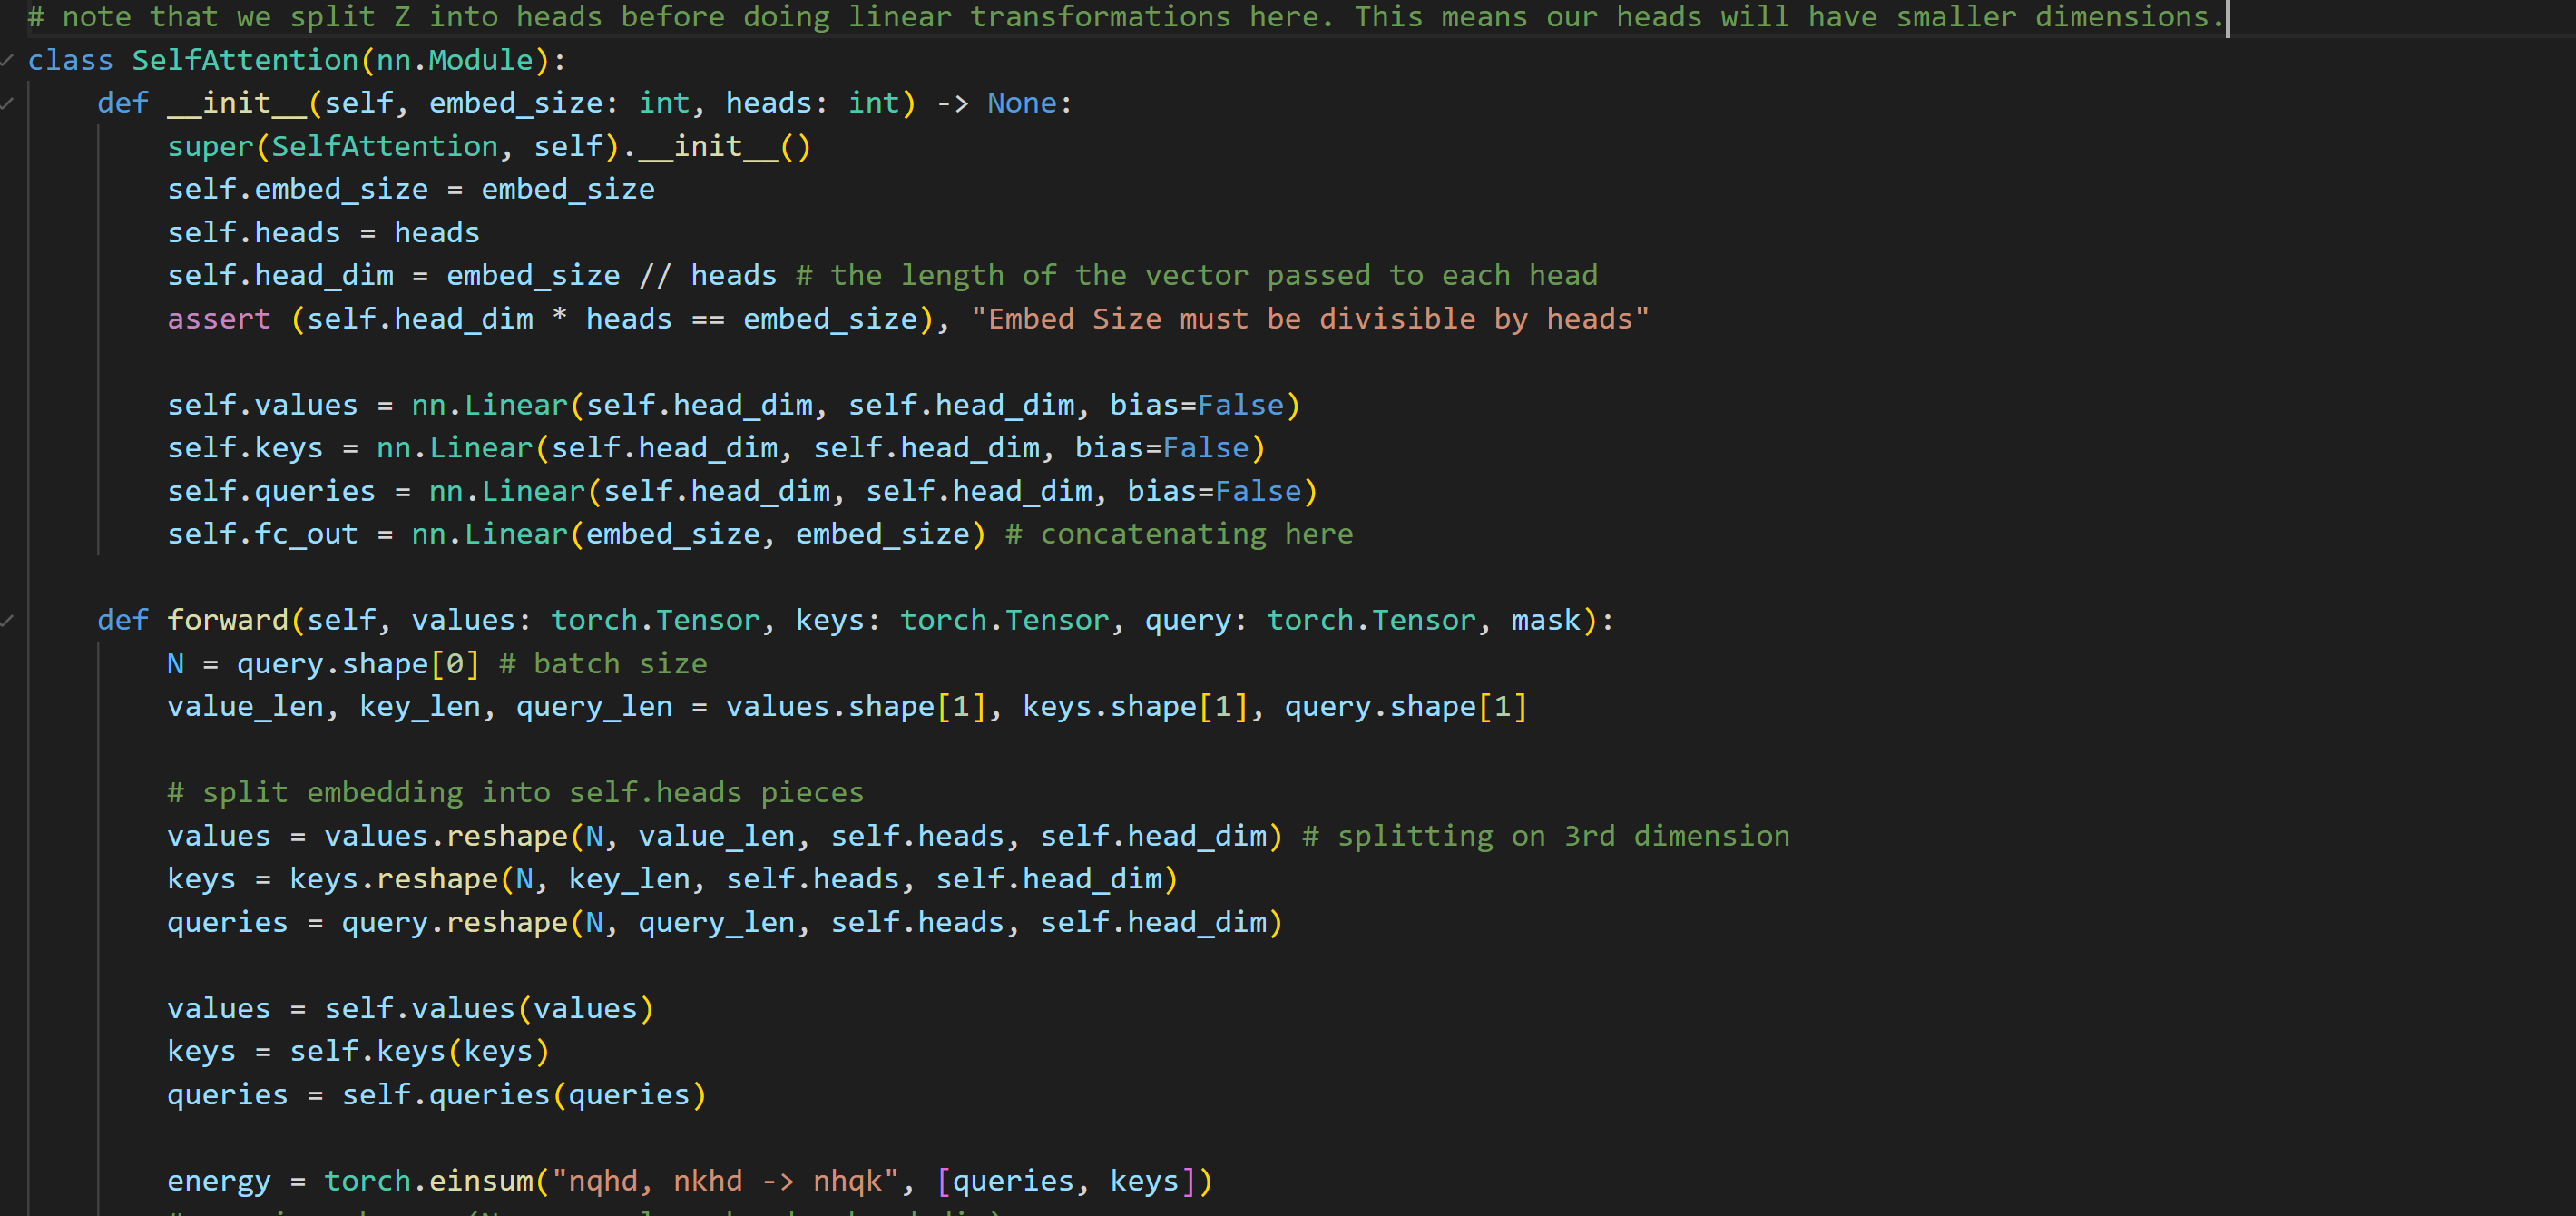
\includegraphics[width=0.8\textwidth]{./attention_small.png}
\end{figure}

This way of doing it is faster because we have substantially less learnable parameters, but can also make for less sophisticated models. Most people (including pytorch) do their linear transformations before splitting into heads: 
\begin{figure}[H]
    \centering
    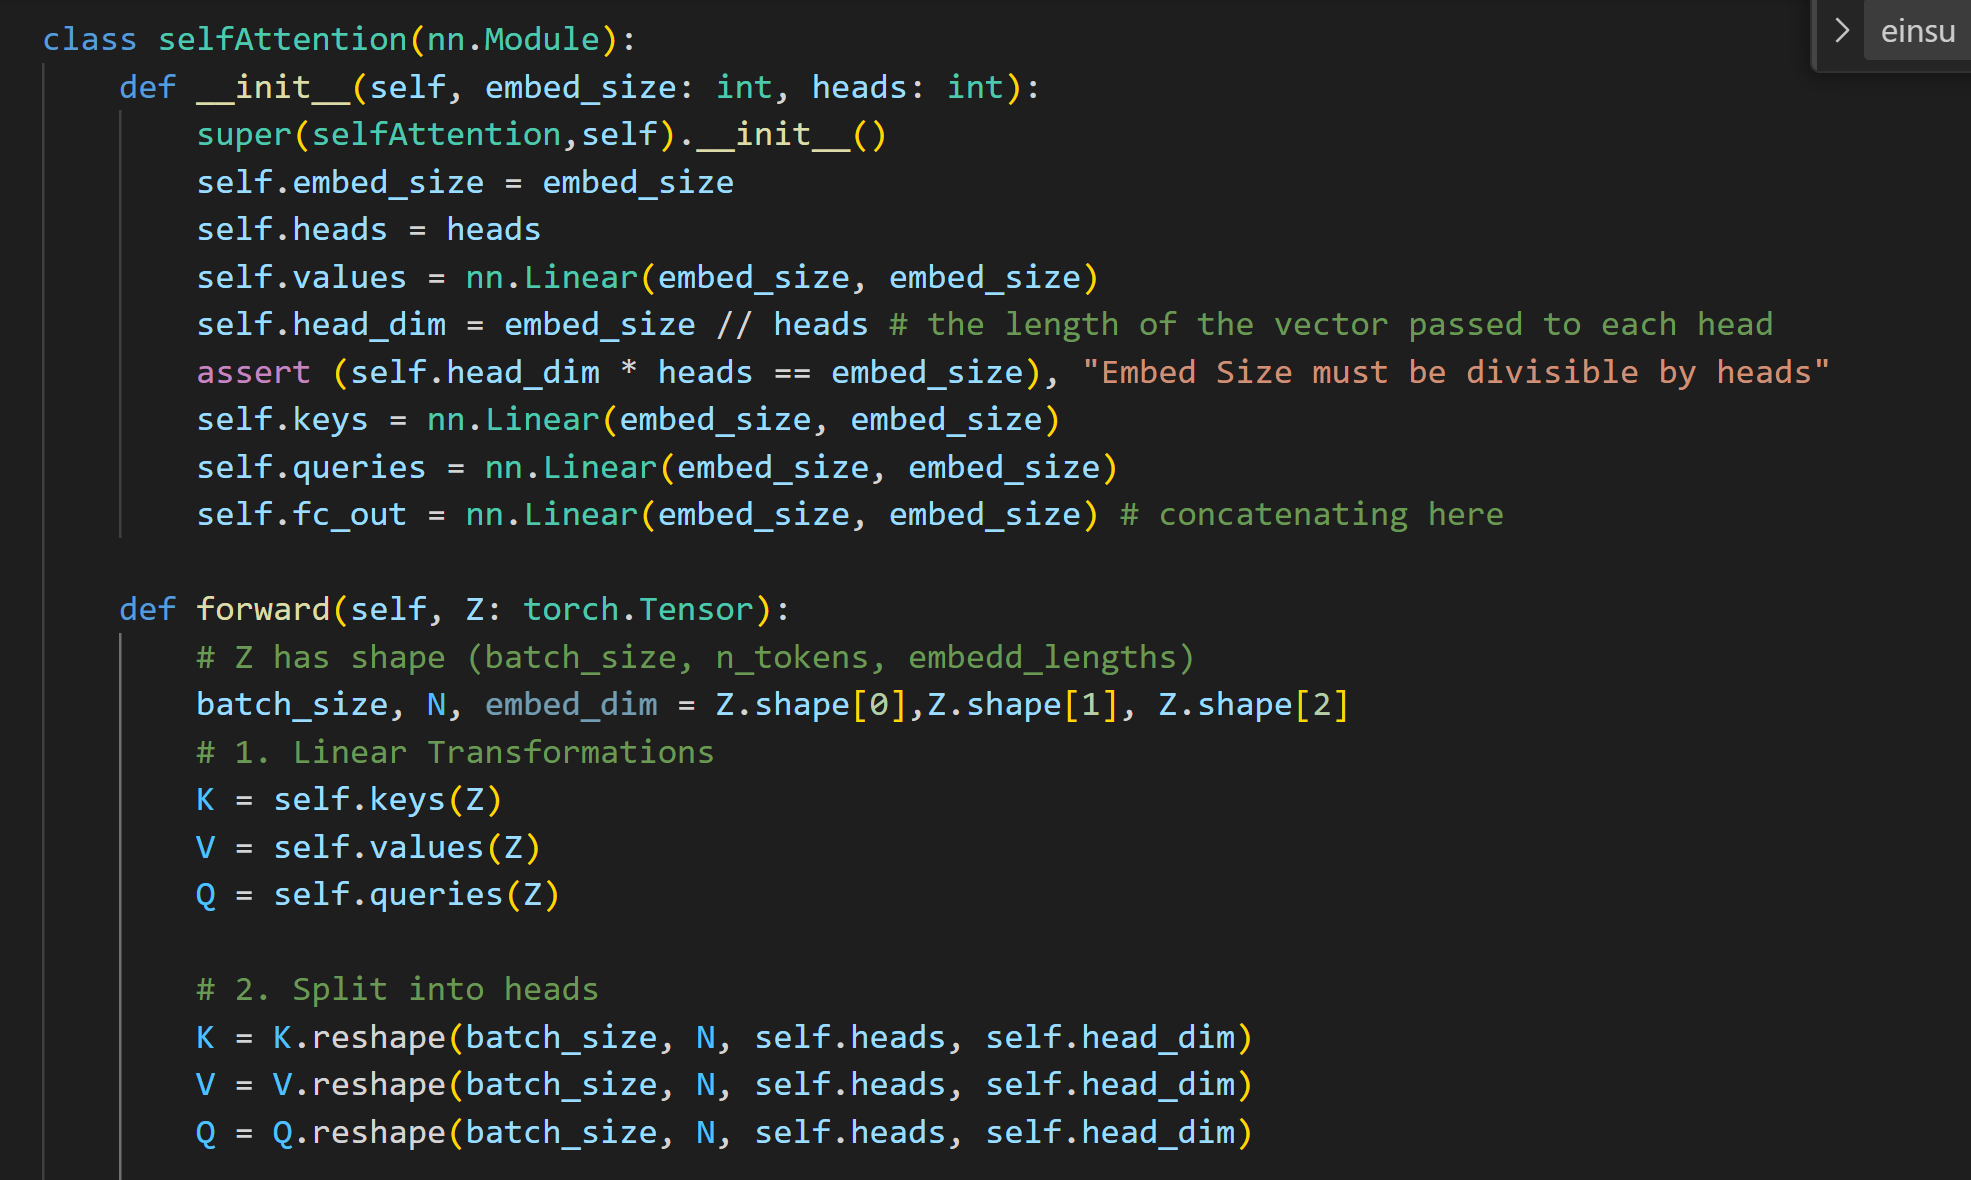
\includegraphics[width=0.8\textwidth]{./attention_big.png}
\end{figure}

\item \textbf{Attention Scores} Now we calculate the attention scores. 

\[
\text{Scores} = \text{Softmax}\left(\frac{QK^T}{\sqrt{d_k}}\right)
\]

The important thing to notice is that our Q and K matrices have shape (ignoring batch size, which would be the first dimension) \(Q, K = [\text{num\_tokens}, \text{head\_dim}]\). So:

\[
QK^T = [\text{num\_tokens}, \text{head\_dim}] \times [\text{head\_dim}, \text{num\_tokens}] \rightarrow [\text{num\_tokens}, \text{num\_tokens}]
\]


This, coupled with the fact that we're taking the inner product of two matrices (think dot product, cosine similarity), means that the attention scores give a measure of the strength of the relationship betwen each pair of tokens! This is similar to a covariance matrix, but it doesn't need to be symmetric and both the Softmax and the \(\sqrt{d_k}\) ensure that its rows sum to 1, meaning each entry in row \(i\) represents the percentage of attention the \(i^{th}\) token should pay to the other tokens, including itself. When we multiply by the values matrix, we then relate the strength of those relationships to the direction the information points us in. In other words, \(\text{Softmax}\frac{QK^T}{\sqrt{d_k}}\) answers the question: How strong is the relationship between token \(i\) and token \(j\). Then multiplying by \(V\) answers the question: what does the strength of this relationship tell us about the meaning of the sentence). 

\begin{figure}[H]
    \centering
    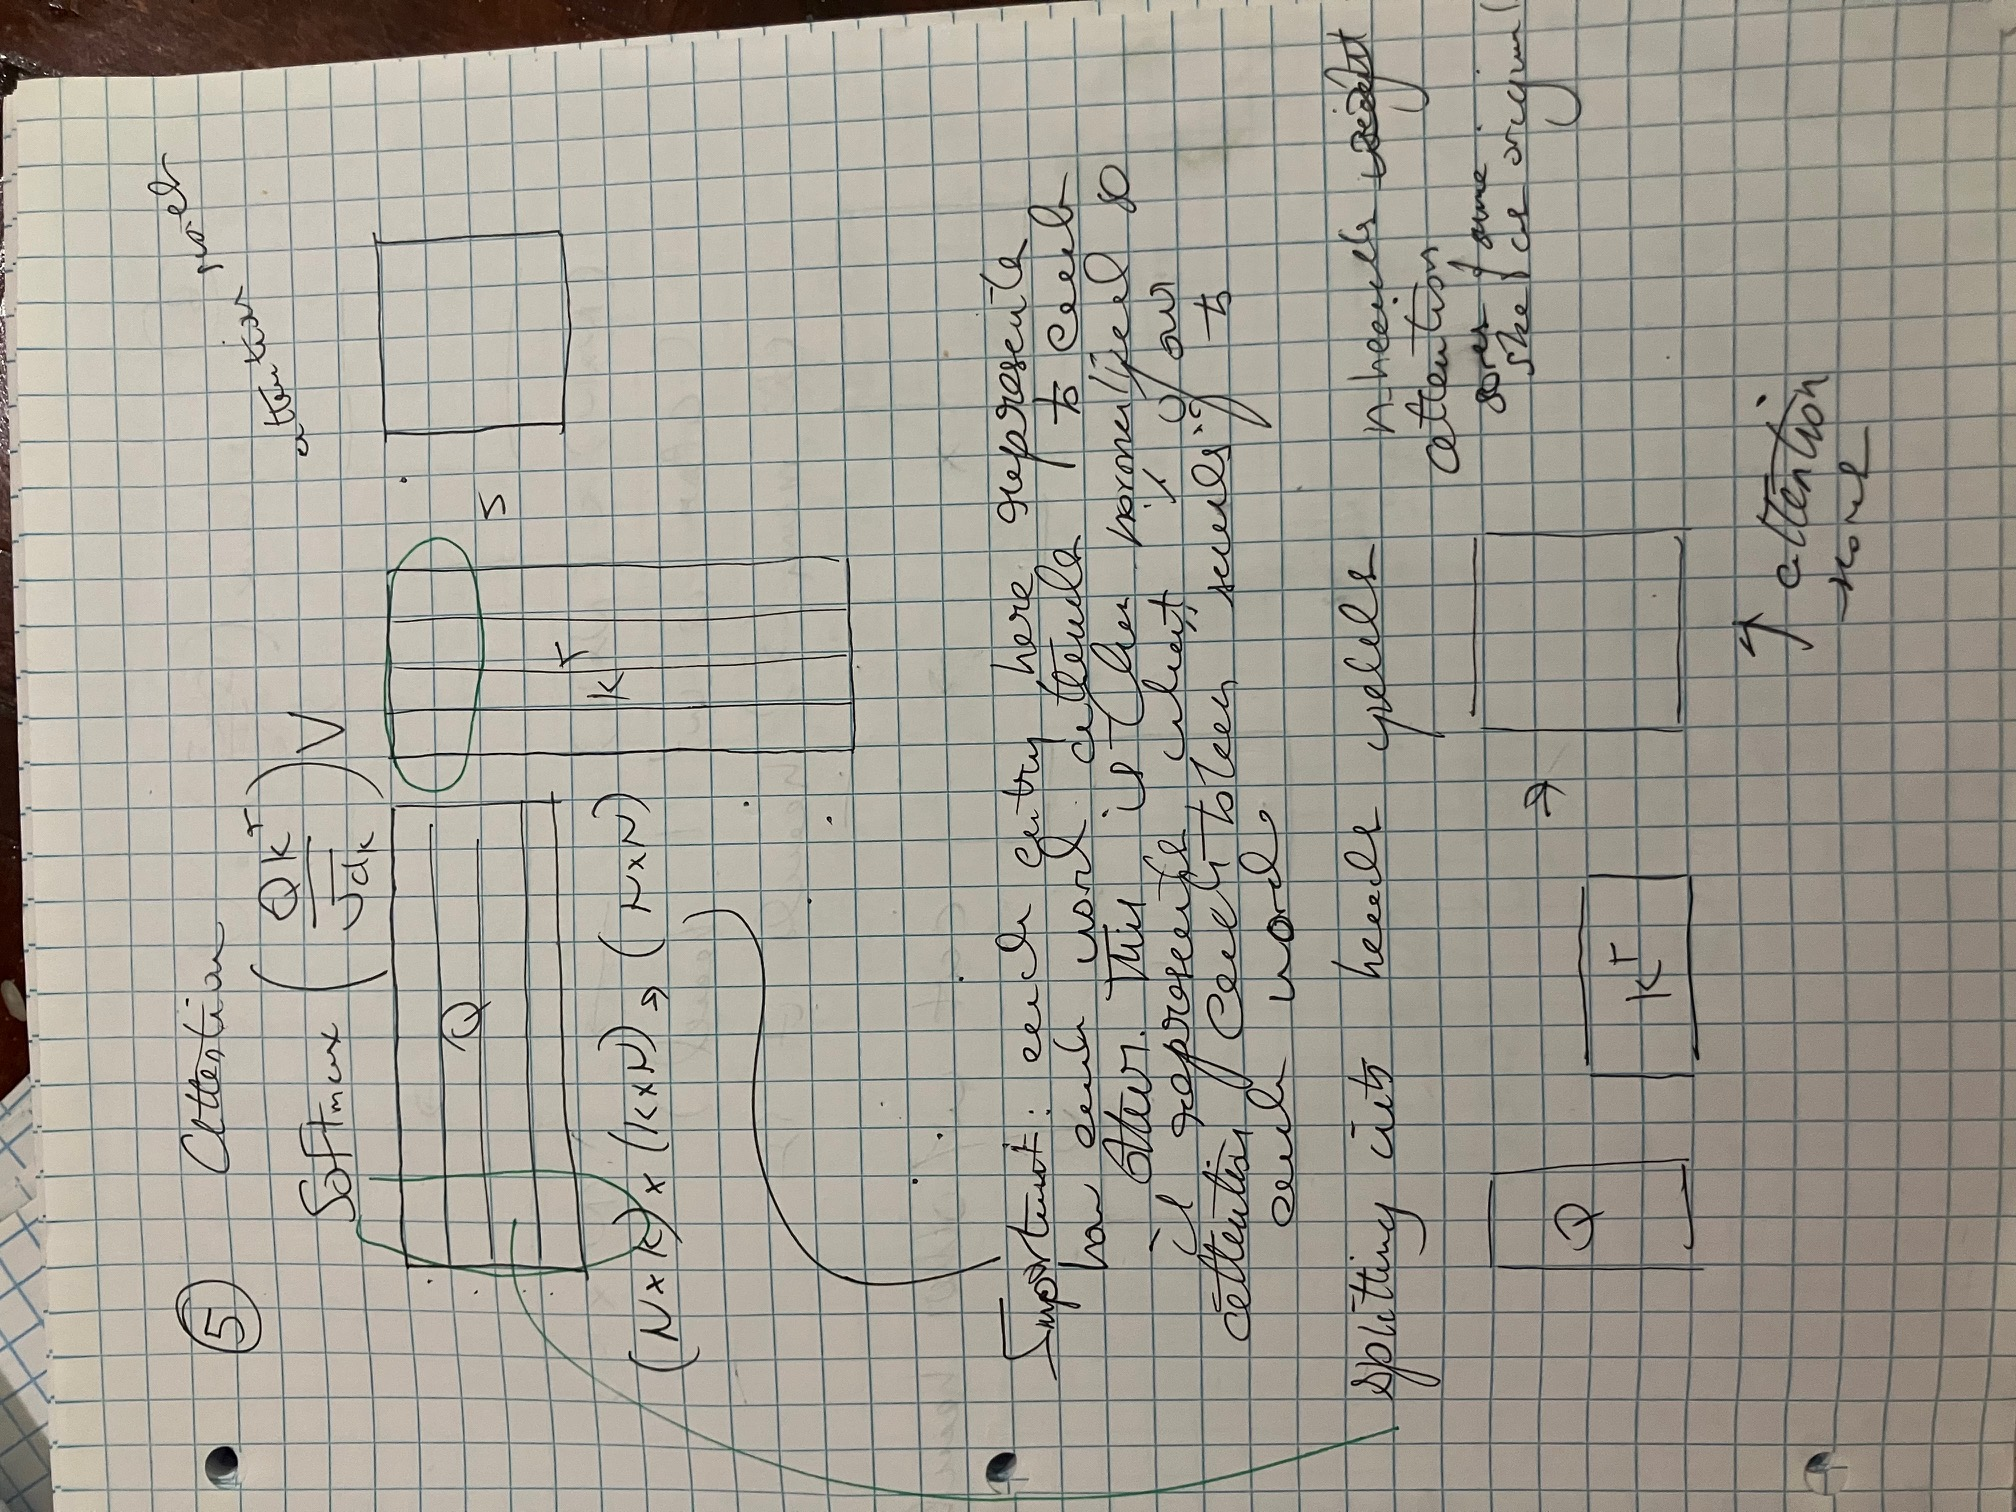
\includegraphics[width=0.8\textwidth, angle=270]{./attention_scores_calculation.jpg}
\end{figure}

\item \textbf{Multiplication by Values Matrix and Concatentation} 
\[\text{Softmax}\left(\frac{QK^T}{\sqrt{d_k}}\right)\cdot V\]

Once the attention scores are calculated, we multiply by the the attention scores from each head by the values matrix for each head. Then we concatenate back together. This works in parallel by splitting the values matrix along its final dimension so that the values associated with each head are stacked vertically. We then multiply them in parallel with the attention scores and concatenate back togehter: 
\begin{figure}[H]
    \centering
    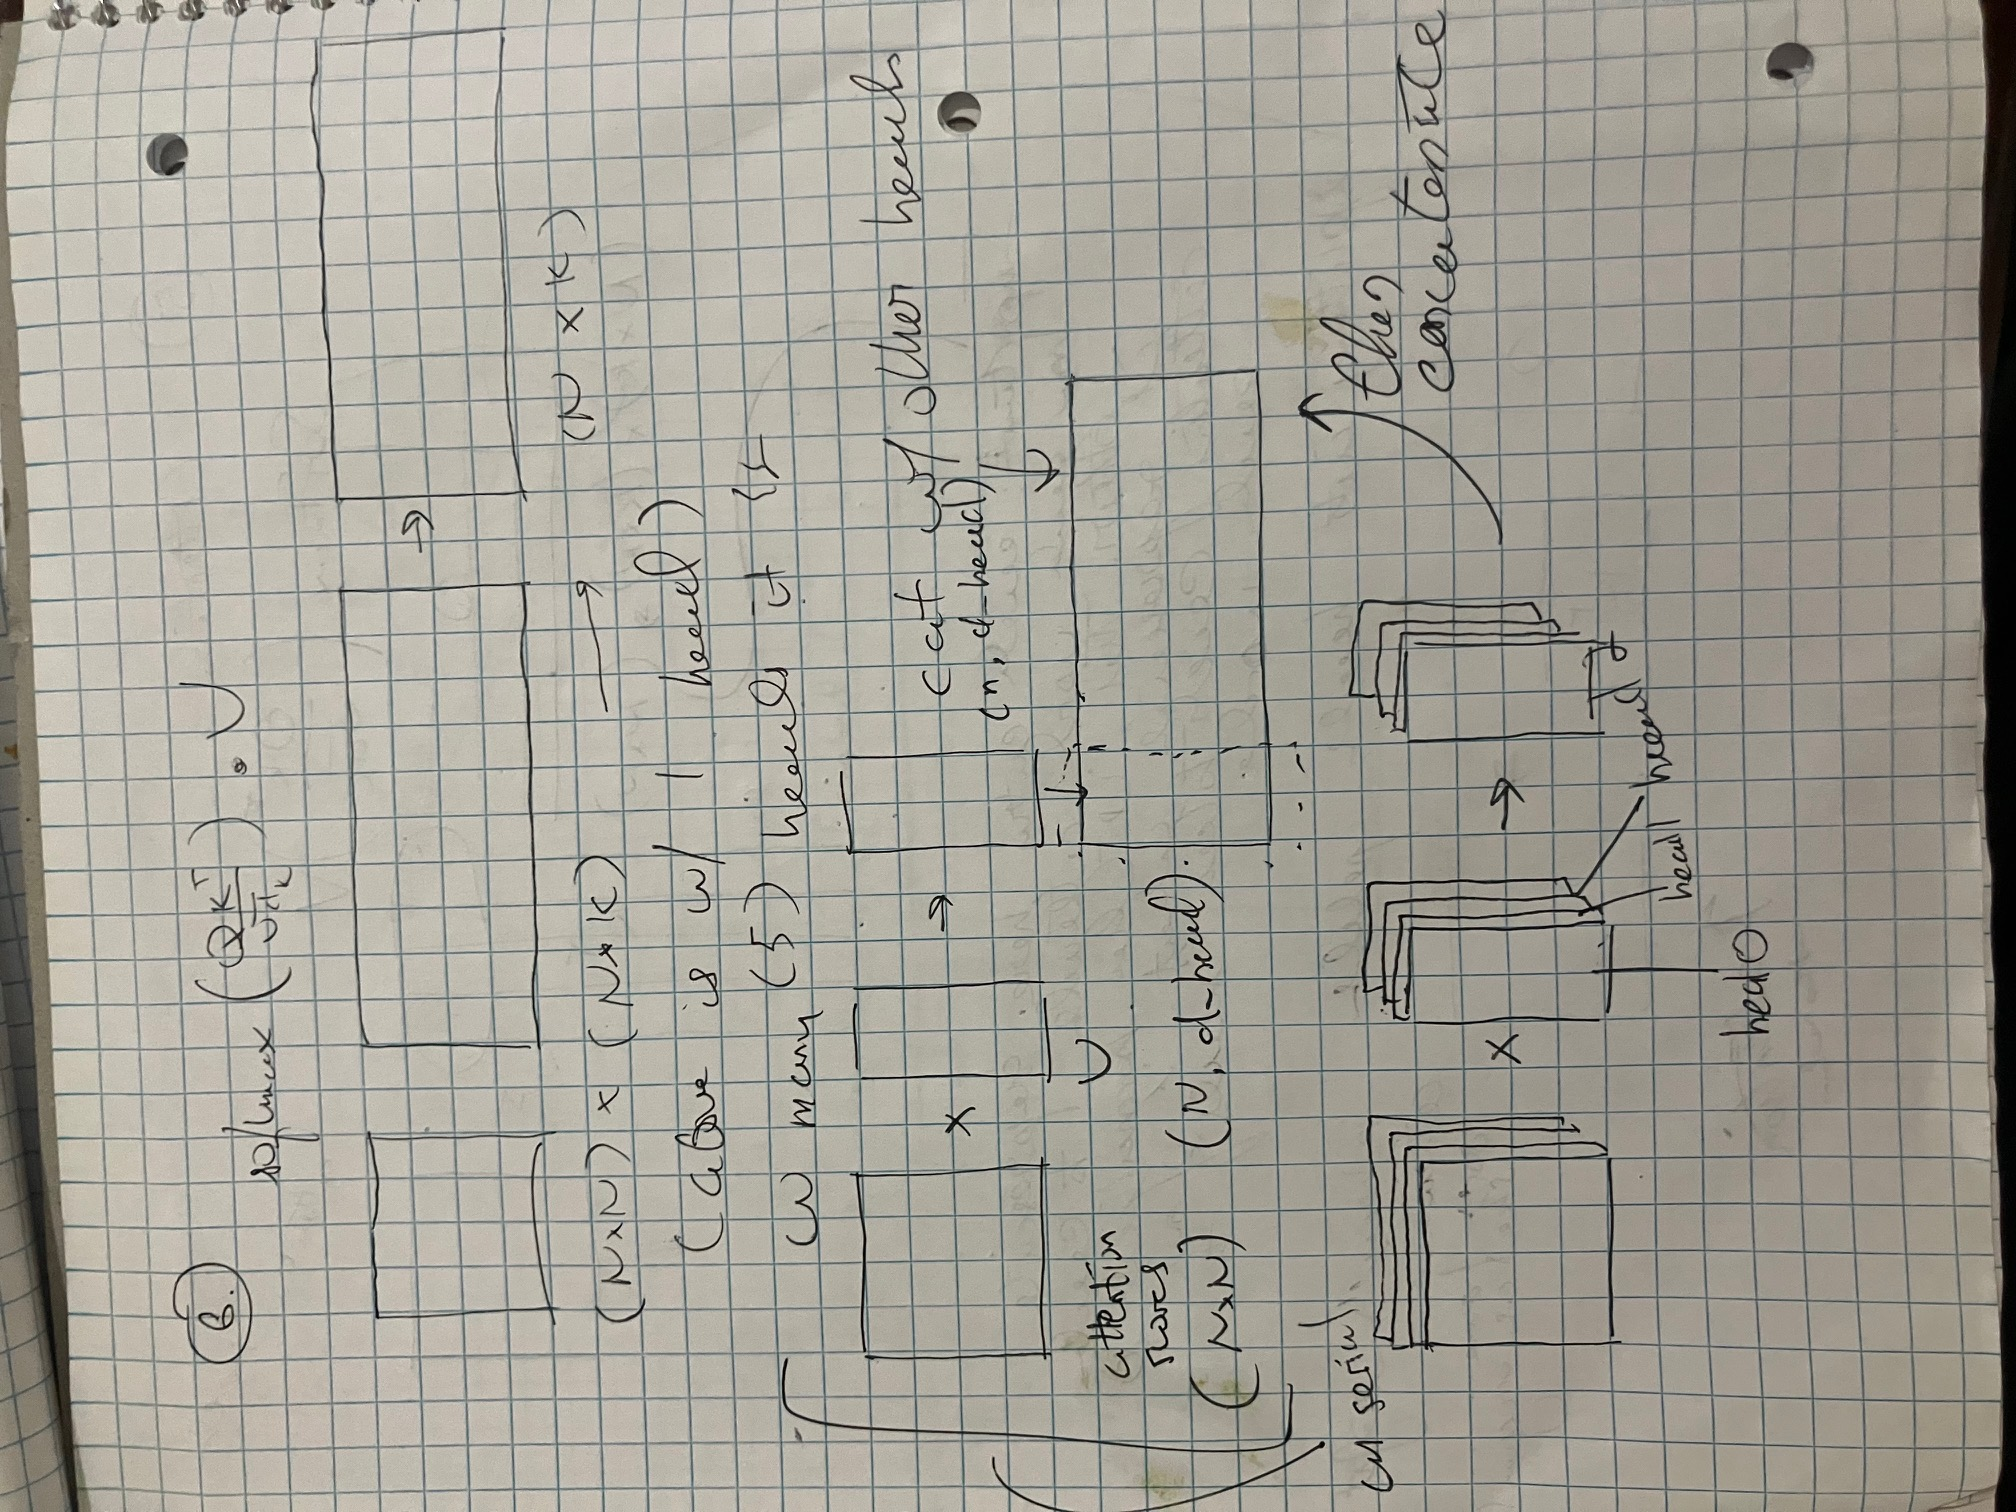
\includegraphics[width=0.8\textwidth, angle=270]{./attention_v_calc.jpg}
\end{figure}
\item \textbf{Feed Forward Neural Network} After going through the self-attention module, the output Z is passed through a feed forward neural network (a simple, two layer perceptron with a relu activation and layer normalization):
\[F' = ReLU(W1 \cdot output) + b1\]
\[F'' = W2 \cdot F' + b2\]

The output  \(F''\)  from this network then gets fed throuh layer normalization and dropout once more, then passed to the next encoder block. And then we repeat this many times and that's the encoder layer of a transformer!
\begin{figure}[H]
    \centering
    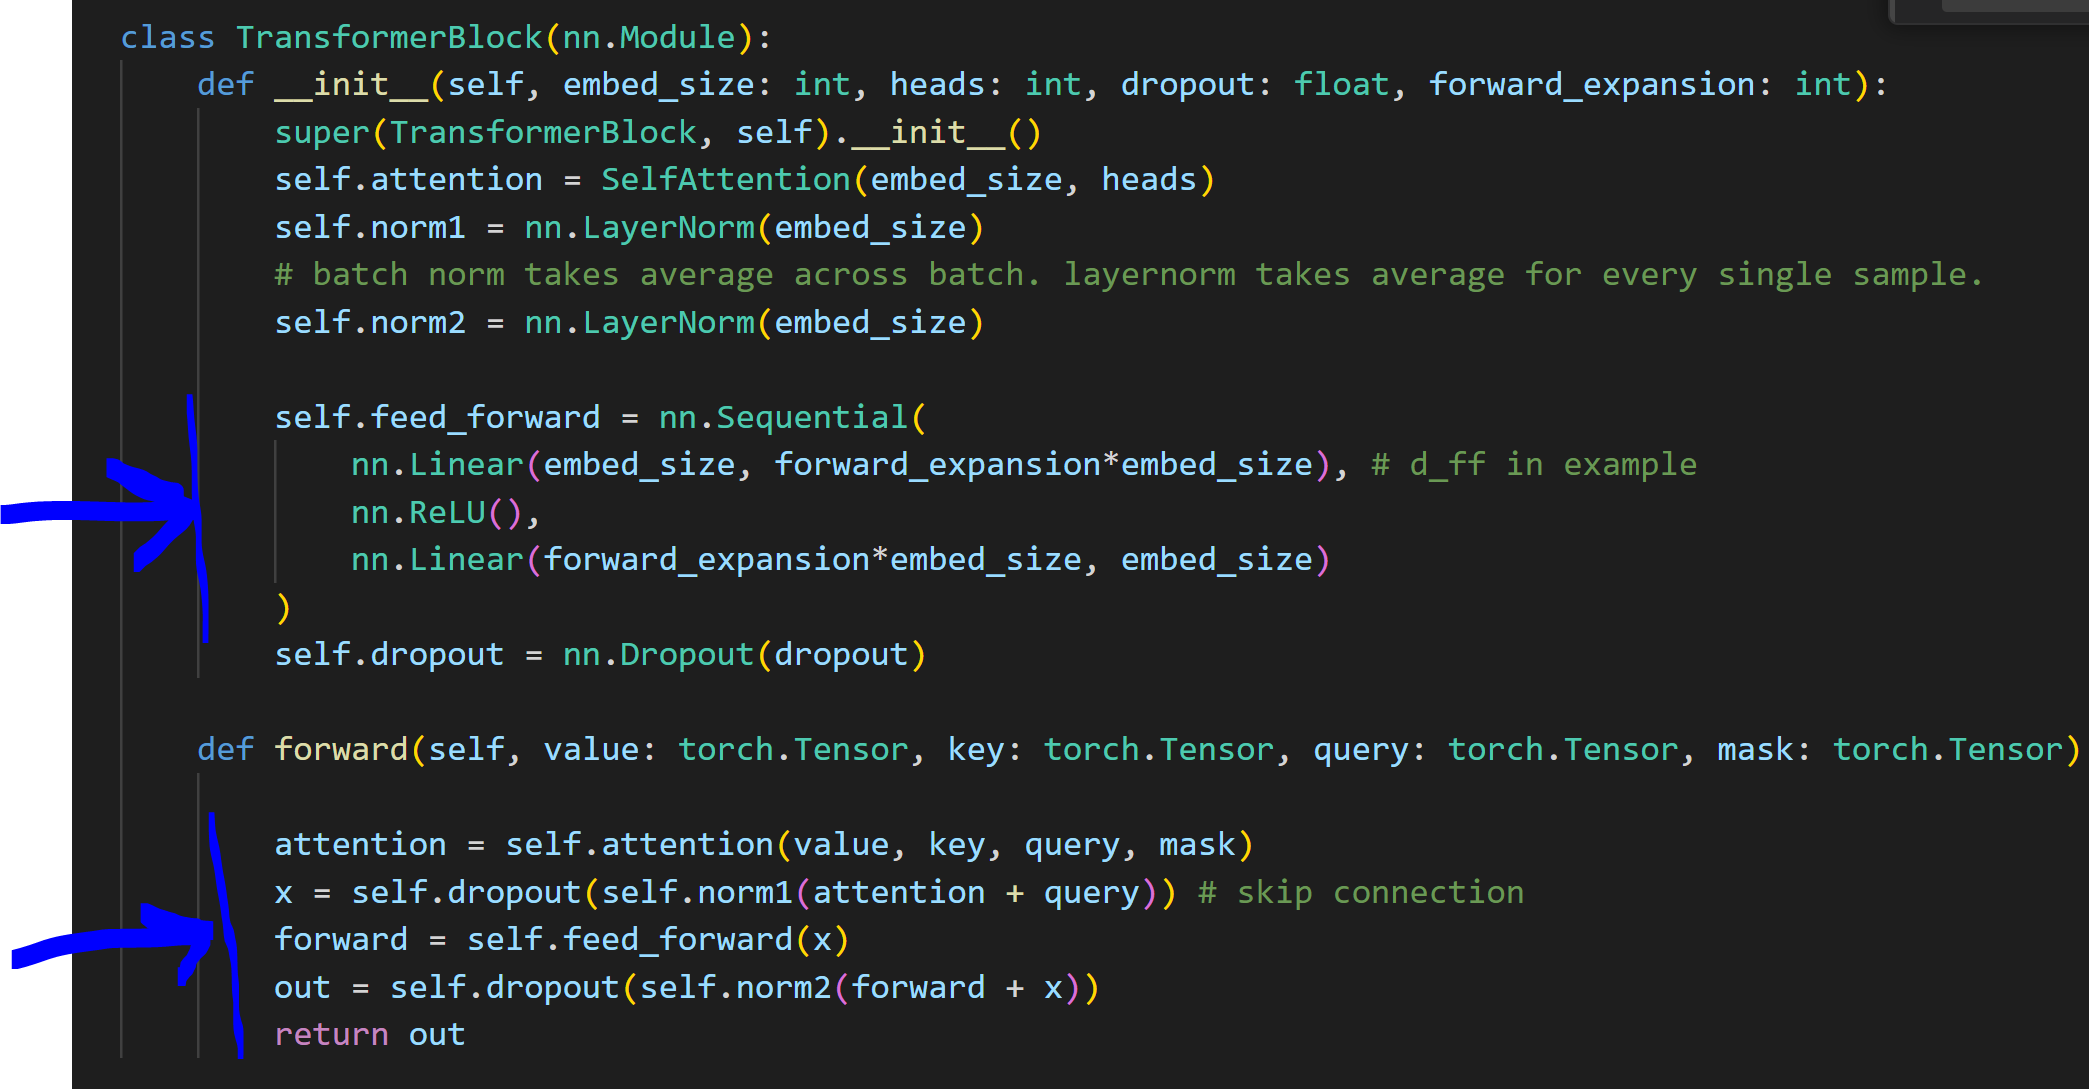
\includegraphics[width=0.8\textwidth]{./ffnn_encoder.png}
\end{figure}
\end{enumerate}


\subsection{Why Does this Work}

\textbf{What is the intuition behind why transformers work?}

\textbf{Why does splitting into multiple heads help?} 
splitting into n heads will result in n attention scores matrices, each one representing the strength of the relationship between tokens when attending to a different portion of the embedding space. When these are concatenated back together, the result is a more fine-grained and sophisticated representation of the relationship between the tokens because we're now attending to different portions of the embedding space individually, rather than doing everything at once. \\

\textbf{What does multiplying by \(V\) actually do?}
The values matrix \(V\) contains the actual data we want to propagate through the network. It holds the information that will be aggregated based on the attention weights. What is literally happening is that we are taking the weighted sum of the value vectors, which means we are modifying the embeddings according to the attention weights, which is to say we are extracting meaning from them.

\[
\text{Output}[i] = \sum_j \text{Attention Weights}[i, j] \times V[j]
\]

I don't think this way of looking at it makes sense, so here is another way (which is completely accurate and looks at the same mathematical process from a different perspective): \\

The attention scores represent the strength of the relationship between each pair of tokens. They answer the question: how strong is the relationship between these two words? Multiplying this by the values matrix relates the strength of these relationships to the information we're trying to learn about the input sentence. The attention scores supply the magnitude, while the values matrix supplies the direction. The values matrix answers the question: what does the strength of the relationships between these tokens mean for what we're trying to learn from this sentence.

\textbf {Why include the Feed Forward Neural Network?}

In a transformer, each encoder and decoder layer includes a subcomponent known as a position wise feed forward neural network. this is the two-layer MLP mentioned briefly above. It's actually very important to overall model performance. This is because the FFN adds considerable capacity to the model without depending on the sequence's context. While the multi-headed attention mechanism effectively captures the contextual relationships within the data, the FFN allows the model to learn more complex functions at each position independently. This is akin to having a powerful, position-specific non-linear transformation applied after considering all contextual information via attention.

\subsection{Decoder}

\begin{enumerate}
\item \textbf{Masked Multihead self-attention}: Looks pretty much the same to the self-attention layers in the encoder. We use our input as the output from the previous layer and run through all the same calculations as above. The only differecne is that we apply a triangular mask to enforce autoregressivity: the guarantee that the model will only generate token \(k\) based on information from tokens \(\{0, 1 ... k-1\}\). This is important because the model will generate incoherent outputs if we don't enforce this. Here is the modified softmax attention equation with the triangular matrix:

\[S  =  \frac{Q_i K_i^T}{\sqrt{d_{head}}} + M\]

Where

\[
M = 
\begin{cases} 
0& \text{if } i \geq j \\
-\infty & \text{if } i < j
\end{cases}
\]

This works because \(softmax(-\infty) \approx 0\), so all future states (where \(i < j\)) will contribute 0 to the final attention score output from the attention module, which is otherwise (aside from \(M\)) the same as that from the attention modules in the encoder: 

\[Attention(Q,K,V) = S \cdot V\]

Where 
\[\sigma(S)_{ij} = \frac{e^{S_{ij}}}{\sum_{k=1}^{n=4}e^{S_{ik}}}\]
\item{\textbf{Multiheaded Cross-Attention Module}}: These are more or less the transformer-equivalent of skip connections. This module follows a self-attention module. Queries come from the previous self-attention module. Keys and values come from the equivalent layer in the encoder. All computation is otherwise exactly the same as a self-attention layer in the encoder. Note: There's no need to mask this out. Since the Keys and Values come from the encoder, their value is already known and hence we don't need to mask and can apply exactly the same computations as the self-attention layers of the encoder
\item{Position-Wise Feed-Forward Networks}: Exactly the same as the feedforward networks in the encoder. Two linear layers with a ReLU in between. No need to belabor the point. 
\item{Residual Connections and layer normalization}: Residual connections (from the beginning of this sublayer) are ported to this point. I neglected to mention it, but each sublayer uses residual connections. Then we sum with the output and do layer normalization. Layer normalization is different from batch normalization. In batchnorm, you take each feature in a batch and average across it for all samples (this is averaging across columns). In layer normalization, you take each sample in a batch and average across it for all features (this is averaging across rows). Then the result of this, which has a standard deviation of 1 and a mean of 0, are sent to the next layer.
\end{enumerate}

\subsection{Loss Function}
Typical loss function for text-generation is categorical crossentropy, where each token represents a class. This means we have a truly extraordinary number of potential classes. This is limited to 10,000 or 50,000 tokens by limited our model to considering a certain number of common tokens, or doing sub-word generation with a slightly more complicated loss function. Essentially, this model is given \(n\) tokens. The loss is calculated like this: after each \(i^{th}\) token, is it able to accurately predict the \((i+1)^{th}\) token. It's really that simple. And it doesn't seem like it should work. But somehow, it does...

\subsection{Pros / Cons}
\textbf{Pros}: 
\begin{enumerate}
\item Not sensitive to problems relating to positional distance between tokens in input
\item No recurrences so its very computationally efficient
\item Anything which can be processed into a vector can be fed into the input (you can use transformers on text, images, text+images
\item Process input tokens simultaneously in parallel, rather than sequentially (more efficient and scalable)
\item Accurately capture contextual information better than other models.
\end{enumerate}
\section{Flash Attention}
Flash Attention is a version of Attention (see transformers section) that is optimized to accelerate attention computation in transformer-based models by reducing memory complexity, while maintaining mathematical equivalence with the standard attention mechanism. \\

Normal self-attention has \(O(n^2d)\) time complexity and \(O(n^2)\) memory complexity, where 
\begin{itemize}
\item \(n\) is the sequence length (T)
\item \(d\) is the embedding dimension (C)
\end{itemize}
Given Queries \(Q \in \mathbb{R}^{n \times d}\), Keys \(K \in \mathbb{R}^{n \times d}\), and Values matrices \(V \in \mathbb{R}^{n \times d}\), the scaled dot product attention is
\[\text{Attention}(Q,K,V) = \text{softmax}\left(\frac{QK^T}{\sqrt{d}}\cdot V\right)\]
where the attention scores \(S\) is
\[
S = \frac{QK^T}{\sqrt{d}} \in \mathbb{R}^{n\times n}
\]
And we apply the softmax row-wise 
\[
P = \text{softmax}(S) \in \mathbb{R}^{n\times n}
\] 
to get the output

\[
\text{Output} = PV \in \mathbb{R}^{n\times d}
\]

In Flash Attention, we do the exact same operations, but instead of storing the entire attention matrix \(S\) and probability matrix \(P\) in memory, we compute them in small "blocks" that fit into fast on-chip SRAM (shared random access memory). Mathematically this looks like: 
% Equation with Sij
\[
S_{ij} = \frac{Q_i K_j^T}{\sqrt{d}}, \quad i, j \in [0, B)
\]
where \( B \) represents the block size that fits into shared memory.

And for the probability matrix equation:
% Pij
\[
P_{ij} = \frac{\exp(S_{ij} - m_i)}{\sum_j \exp(S_{ij} - m_i)}
\]
where \( m_i \) is the row-wise maximum for numerical stability.

% 2x2 table showing comparison of time and space complexity for standard self-attention and flash attention
\begin{table}[h]
\centering
\begin{tabular}{|c|c|c|}
\hline
\textbf{Method} & \textbf{Time Complexity} & \textbf{Space Complexity} \\
\hline
Standard Self-Attention & \( O(n^2 d) \) & \( O(n^2) \) \\
\hline
Flash Attention & \( O(n^2 d) \) & \( O(n) \) \\
\hline
\end{tabular}
\caption{Comparison of time and space complexity between standard self-attention and Flash Attention.}
\end{table}

This means that we asymptotically improve our memory requirements while preserving mathematical equivalence and without harming our asymptotic time complexity.\\

\textbf{Question}: Why does this not reduce model parallelism by introducing serial operations? Surely the blocks are computed sequentially...\\

\textbf{Answer}: The blocks can be worked on in overlapping stages across different GPU processing units, with different blocks of the attention and probability matrices \(S\) and \(P\) at different stages of the pipeline at different times. This means that we substantially reduce our memory complexity, but our time complexity is unchanged and serial operations are avoided. \\

In fact, while this algorithm doesn't change the asymptotic time complexity for the algorithm (it only asymptotically reduces the space complexity), in practice, optimizing the block size to fit in with SRAM means that we get substantial practical improvements in processing \emph{time} as well. 
\textbf{Question}: Block size and sequence length don't necessarily line up. Block size is optimized for the hardware we're running on and may be lesss than the sequence length (in theory). So how does the softmax get computed if sequence length and block size don't cleanly match up? \\ 
\textbf{Answer}: First, computing the attention scores is easy. If block size is less than seq length, we compute the attention scores for some subset \(S_{i:i+B, j:j+B}\) of the attention scores matrix. We have an ironclad guarantee that this \emph{portion} of the attention scores matrix is computed completely and correctly. \\
Computing \(P\) is trickier, because we may not make it all the way through a row. This means we need a way to handle \emph{incomplete overlaps} in rows of \(P\) while maintaining numerical correctness and algorithmic efficiency. How does this happen?
To handle incomplete overlaps in the softmax computation, FlashAttention processes the softmax in an incremental manner across blocks while maintaining numerical stability.

First, within each block, we compute a local maximum for numerical stability:

\[
m_{\text{local}, i} = \max_{j \in \text{block}} S_{ij}
\]

As additional blocks are processed, we update the global row-wise maximum incrementally:

\[
m_{\text{global}, i} = \max(m_{\text{global}, i}, m_{\text{local}, i})
\]

Once all blocks are processed, the final softmax normalization is applied using the global maximum:

\[
P_{ij} = \frac{\exp(S_{ij} - m_{\text{global}, i})}{\sum_j \exp(S_{ij} - m_{\text{global}, i})}
\]

Handling value aggregation also requires incremental accumulation across blocks:

\[
O_i = \sum_j P_{ij} V_j
\]

Each block processes partial results, and the final output is obtained after all relevant blocks have been processed.

This approach ensures that although the computation is broken into smaller chunks, the final result is mathematically equivalent to full attention computation across the entire sequence. The algorithm processes different blocks in a streaming fashion, allowing for efficient memory usage without sacrificing accuracy.

\section{Mixture of Experts (MoE) Model}
A MoE is a more compute-efficient innovation on the typical transformer model that involves modifying the Feed Forward Network (FFN) layers of a LLM. Specifically, each dense FFN Layer is replaced with a sparse MoE FFN layer, which is composed of a gate network and a certain number of experts. The gate network is composed of learned parameters and is pretrained at  the same time as the rest of the network. The experts are a series of smaller FFNs. At train time and at inference time, the learned router directs specific tokens to be processed by only a subset of the total parameters present in the FFN layer. Each one of these distinct subsets is called an "expert" and is a full, unique FFN. A single token can be attended to by one or more experts. 

\begin{figure}[H]
    \centering
    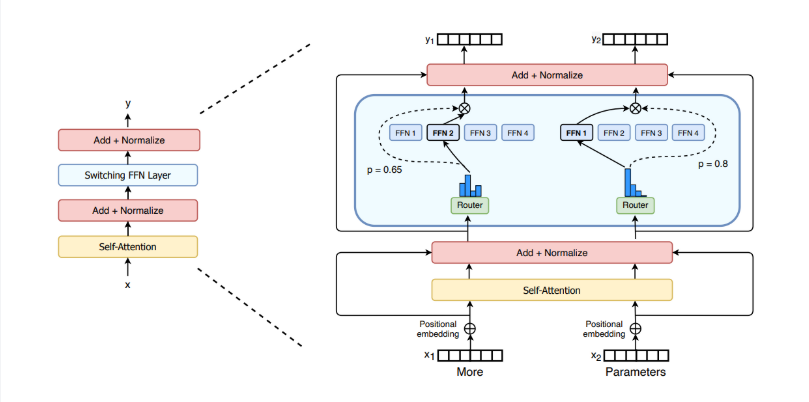
\includegraphics[width=1.0\textwidth]{./moecircuit.png}
\end{figure}

\textbf{This is great. But what does it do?}:\\
the FFN layers in a decoder-only transformer will typically be 60\%-80\% of the total model parameters. Maknig the model sparser by using only a fractin of them at train and at inference time leads to substantial improvements in pretraining and inference time compute efficiency. Unfortunately, though, MoE models also exhibit substantial instability with post-training and also struggle to generalize unless they are pretrained very carefully. There are a couple of reasons why this is the case: 
\begin{enumerate}
\item \textbf{Batch Size / Pretraining Inconsistencies}: Because MoE routers direct certain tokens to certain experts and are learned alongside the model during pretraining, the tokens-per-batch is not constant per expert or throughout the pretraining process. This introduces an inherent instability into the model
\item \textbf{Virtual Circuits / Interpretability take}: Transformers are already extremely sparse networks. There's also a sense in which they are lower-dimensional projections of even larger, sparser networks; there are clearly virtual circuits inside neural networks, and these virtual circuits clearly share parameters. The existing sparsity inside neural networks means there are absolutely gating mechanisms being learned by the model parameters, directing the flow of information to certain circuits (virtual experts) and not others, depending on the attention scores of each token. I think MoE's are imposing an artificial partition upon these networks which lkely limits their exprsesiveness as well. \textbf{Note}: this is just a guess of mine. GPT-o1 says "This claim is speculative but not without merit." So take this second point with a grain of salt.
\end{enumerate}
In spite of these limitations, their lower latency and compute requirements mean they're an interesting idea, and I'm sure there will be further innovations to the FFN in transformers going forwards.

\section{Tokenization}
This section covers the tokenization process for language models. We cover the root algorithm (Byte-Pair Encoding) and then discuss how this is applied to the GPTNeoXTokenizer after that. 
\subsection{Byte-Pair Encoding}
Byte-pair encoding is a data compression algorithm dating to 1994 that is used today in the tokenizers for most LLMs. Here is an algorithmic walk-through:

Let's assume we have the following string of characters we want to encode (this is from the example on Wikipedia): 
\[[\text{aaabdaaabac}]\]
\begin{enumerate}
\item Assume all unique characeters belong to an initial set of 1-character long n-grams, the initial tokens: \\
\[[\text{"a", "a", "a", "b", "d", "a", "a", "a", "b", "a", "c"}]\]
\item Then repeatedly assign the most frequent pair of adjacent characterse to a new 2-character long n-gram and all instances of that pair are replaced by that new token. The most common 2-character long ngrams are "ab" and "aa". We pick "aa" arbitrarily: \\
\[[\text{"Z", "a", "b", "d", "Z", "a", "b", "a", "c"}]\]
\item Maintain a replacement table recording all the transformations you made. Our replacement table is:
\[[\text{"Z"  = "aa"}]\]
Let's repeat a few more times so you get the idea:
\[[\text{"Z", "Y", "d", "Z","Y", "a", "c"}]\]
And our replacement table is:
\[[\text{"Z"  = "aa", "Y" = "ab"}]\]
\item Repeat this process until you've reached a specified vocab size or can't compress the data any further. 
\end{enumerate}
\subsection{GPTNeoXTokenizer}
This is how GPTNeoXTokenizer works:

\begin{enumerate}
\item \textbf{UTF-8 Encoding}: First, we encode all characters in the text by their ASCII values. \\
\begin{itemize}
\item For example, "Hello" becomes \([72, 101, 108, 108, 111]\)
\item Non ASCII characters like ñ get replaced by their UTF-8 Encoding, which goes from 0-255.
\item In UTF-8, ASCII values are mapped from 0-127. Continuation bytes are 128 - 191.  Leading bytes for non-ASCII characters are 192-255. 
\item All non-ASCII characters are represented by two bytes consisting of a leading byte and continuation byte character.
\item For example, ñ is represented by \([195, 177]\). The Ġ token represents whitespace.
\end{itemize}
\item \textbf{Pre-Tokenization}: Before tokenizing, the pre-tokenizer splits byte sequences into basic units, usual by whitespace. \\
\begin{itemize}
\item For examle, " GPT-3 is great!" might be split into: ["ĠGPT", "-", "3", "Ġis", "Ġgreat", "!"]
\item \textbf{Note}: Pre-tokenized units ar enot fixed! You don't have to respect the boundaries of the pre-tokenized units when doing byte pair encoding. The pre-tokenization step is more about splitting the input text into initial units that are easier to woprk wtih, like white-space separated words, punctuation marks, and special characters.
\end{itemize}
\item \textbf{Byte-Pair Encoding}: Now, we do byte-pair encoding as described above. We start off with a huge number of byte-sequences, and decrease these through merges until we reach some predefined number of words, our vocab\_size.
\item \textbf{Vocabulary Lookup} At this point we have vocab\_size tokens. The tokens are now "looked up" into the vocabulary (they are mapped to a unique integer, and then token, integer pair gets stored in the tokenizer dict).
\item \textbf{Post-Processing} Adding of special tokens ([UNK] [CLS] [SEP]) get added. These are used to structure text inputs for the model. 
\begin{itemize}
    \item For example, the token \textless|endoftext|\textgreater{} is defined in the Pythia language models delimiting the end of input text. It signals the model to stop generating further tokens.
    \item \textless|padding|\textgreater{} is used to pad sequences to a fixed length when batching input samples of different lengths.
\end{itemize}
\end{enumerate}
\textbf{Question}: How does GPTNeoXTokenizer prevent partial merges during the Byte-Pair Encoding process? \\
First, a partial merge is where a non-ASCII character has its leading or continuation byte merged with a neighboring character during BPE, but not the other. The result is an encoding where there's now a byte that doesn't correspond to anything in language dangling, and a merge that doesn't either. This is prevented because the BPE algorithm knows to the values of leading and trailing bytes for non-ASCII characters, and it's coded not to split them up.\\

\textbf{Note}: Language processing techniques like stemming and lemmatization are NOT used by GPTNeoXTokenizer (See Definitions and Tips section for an explanation of Stemming and Lemmatization).

\section{Neural Scaling Laws (Kaplan et. al 2020)}
\textbf{Note}: This is without a doubt the most important LM research paper published since "Attention is All You Need" (Vaswami, 2017).  The authors define a set of neural scaling laws that hold for training LLMs. I will define the power laws and describe them. Then I will describe how to apply them practically to ML problems

\subsection{The Power Laws}
The paper introduces a general form for scaling laws:

\[\mathcal{L}(X) = \left(\frac{X_0}{X}\right)^\alpha + \mathcal{L}_\infty\]


These scaling laws hold for the number of non-embedding model parameters \(N\), the dataset size in tokens \(D\), and the total amount of compute time available in PetaFLOP-Days \(C\). \\

\textbf{Basically this means that if two of these three factors are unlimited, the loss \(\mathcal{L}\) will scale linearly (in log-space) as a function of the third}:

\[\mathcal{L}(N) = \left(\frac{N_0}{N}\right)^{\alpha_N} + \mathcal{L}_\infty; \quad N_0 \sim 8.8 \times 10^{13}, \alpha_N \sim 0.076\]
\[\mathcal{L}(D) = \left(\frac{D_0}{D}\right)^{\alpha_D} + \mathcal{L}_\infty; \quad D_0 \sim 5.4 \times 10^{13}, \alpha_D \sim 0.095\]
\[\mathcal{L}(C) = \left(\frac{C_0}{C}\right)^{\alpha_C} + \mathcal{L}_\infty; \quad C_0 \sim 3.1 \times 10^8, \alpha_C \sim 0.050\]
The constant \(\mathcal{L}_\infty\) is an irreducible loss constant owing to the fact that language has nonzero entropy, and the other terms are empirically derived constants.

\begin{figure}[H]
    \centering
    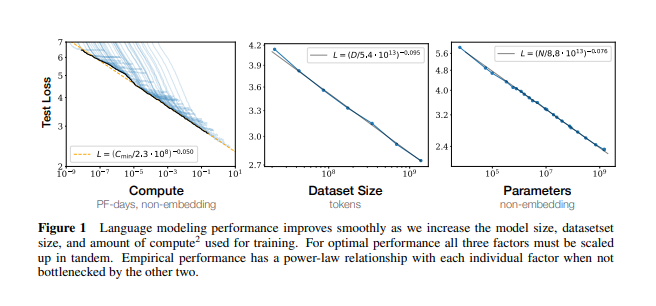
\includegraphics[width=0.8\textwidth]{./powerlaws_graph.png}
\end{figure}

\textbf{If parameter size \(N\) and one other variable are jointly limited, while the third remains unlimited, the loss \(\mathcal{L}\) will scale as a function of the other two parameters}:
\[\mathcal{L}(N,D) = \left[\left(\frac{N_c}{N}\right)^{\frac{\alpha_N}{\alpha_D}} + \frac{D_C}{D}\right]^{\alpha_D}\]


\subsection{Critical Batch Size}
Let's say we have some target loss \(\mathcal{L}_{targ}\) we want to achieve. Critical Batch size \(B_{\text{crit}}\) is the batch size where the training regime transitions from being step-limited to compute limited:

\[B_{\text{crit}}(\mathcal{L}_{targ}) \approx \frac{B_{*}}{\mathcal{L}_{targ}^{\frac{1}{\alpha_B}}}\]

Where \(B_{*} \approx 2 \times 10^8\) and \(\alpha_B \approx 0.21\) \\

\begin{itemize}
\item If you're below \(B_{\text{crit}}\), the model's performance is primarily driven by the number of steps \(S\). Therefore we should try to minimize the number of steps \(S\) it takes to reach our target loss  \(\mathcal{L}_{targ}\).
\item If you're above \(B_{\text{crit}}\), the model's performance is primarily driven by the total amount of compute \(C\) available, so we should try to minimize the number of PetaFLOPs \(C\) required to reach our target loss \(\mathcal{L}_{targ}\).
\item \textbf{Note}: You should always aim for being as close to B crit as possible, because if your batch compute-limited you will be below \(B_{\text{crit}}\), and you should increase B to reduce gradient noise and minimize steps. Meanwhile if you're above \(B_{\text{crit}}\), you should keep B near \(B_{\text{crit}}\) because increasing it beyond that incurs additional computational costs at the expense of throughput. So you're reducing the amount of useful compute that is done above \(B_{\text{crit}}\) and given some high but fixed computational budget.
\end{itemize}



Neural scaling laws refer to a set of laws discovered by Kaplan et. al in 2020 pertaining to training LLMs. Below, I summarize and explain the laws and how they can be applied to the practical training of LLMs.\\

The essential finding is that the performance \(\mathcal{P}\) of an LLM can be expressed as follows:

\[
\mathcal{P} = k \cdot N^\alpha \cdot D^\beta \cdot C^\gamma 
\]
Where 
\begin{itemize}
\item \(k\) is a constant that depends on the specific model and task
\item \(\alpha\), \(\beta\), and \(\gamma\) are constants that characterize the relationship between performance and each scaling factor
\item \(N\) is the number of non-embedding model parameters
\item \(D\) is the size of the dataset in tokens
\item \(C\) is the amount of compute allocated to training in petaflop days. 
\end{itemize}
In other words, when we scale \(N\), \(D\), and \(C\) in common we can expect constant improvements in the loss for language models. 
\begin{figure}[H]
    \centering
    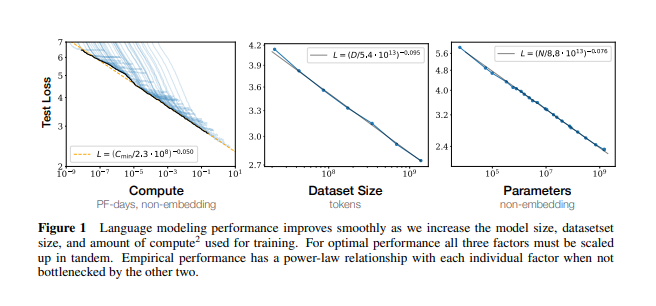
\includegraphics[width=0.8\textwidth]{./powerlaws_graph.png}
\end{figure}

\textbf{Petaflop-Day}: Flop = Floating Point Operations Per second. It gives the number of calculations a computer can perform per second. A petaflop = \(10^{15}\) floating point operations per second. A petaflop-day equals one machine doing \(10^{15}\) floating point operations per second for a whole day.\\

This scaling law above means that if you hold any two of these factors constant, there is a direct proportional relationship between test loss \(\mathcal{P}\) of an autoregressive LLM and the remaining factor:

\begin{enumerate}
    \item For models with a limited number of parameters \(N\), trained to convergence on sufficiently large datasets:
    \[
    L(N) = \left(\frac{N_c}{N}\right)^{\alpha_N}; \quad \alpha_N \sim 0.076, \quad N_c \sim 8.8 \times 10^{13} \text{ (non-embedding parameters)} \tag{1.1}
    \]
    
    \item For large models trained with a limited dataset \(D\) with early stopping:
    \[
    L(D) = \left(\frac{D_c}{D}\right)^{\alpha_D}; \quad \alpha_D \sim 0.095, \quad D_c \sim 5.4 \times 10^{13} \text{ (tokens)} \tag{1.2}
    \]
    
    \item When training with a limited amount of compute, a sufficiently large dataset, an optimally-sized model, and a sufficiently small batch size (making optimal use of compute):
    \[
    L(C_{min}) = \left(\frac{C_{min}}{C_{min}}\right)^{\alpha_C^{min}}; \quad \alpha_C^{min} \sim 0.050, \quad C_{min} \sim 3.1 \times 10^8 \text{ (PF-days)} \tag{1.3}
    \]
\end{enumerate}



Here are some other key findings from their paper (explained if I feel they need explaining):
\begin{itemize}
\item \textbf{Model Depth Doesn't Matter (as long as \(n_{layers}\geq 3\))}: The depth of the model does not significantly impact performance. All that matters is the number of non-embedding parameters. (fat and shallow LLMs will perform as well as narrow and deep ones, as long as you don't get carried away) 

\begin{figure}[H]
    \centering
    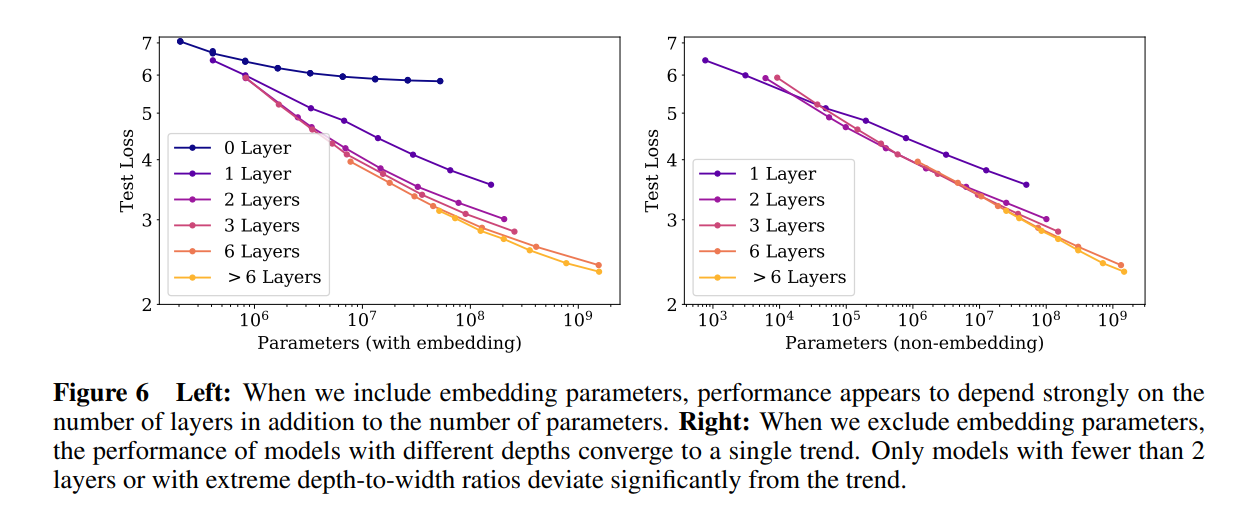
\includegraphics[width=0.9\textwidth]{./depth_performance.png} % Adjust the width as needed
\end{figure}

\item \textbf{Performance depends only mildly on model shape when the total number of non-embeddings parametrs \(N\) is held fixed}: The following fields don't matter:
\begin{enumerate}
\item \textbf{Feed-Forward Ratio}: If the input \(Z\) to a self-attention layer has shape (B,T,C), where B = batch size, T = context length, and C = num channels, C is the width of the self attention layer and then k * C where k is some constant gives the width of the ffnn following that layer. So in this case the \textbf{Feed Forward Ratio} = \(k\). K can be between 4 and 100 without significantly impacting performance.
\item \textbf{Aspect Ratio}: Aspect ratio gives the ratio between C and \(n_{layers}\). C can be between 10 and nearly 500 without significantly impacting performance
\item \textbf{Attention Head Dimension}: Attention head dimension can be between 10 and well over 100 without much of a performance impact. This is true regardless of what C is (256, 512, or 1024), though anecdotally it appears large C generally do best with larger head dimensions.
\end{enumerate}
\begin{figure}[H]
    \centering
    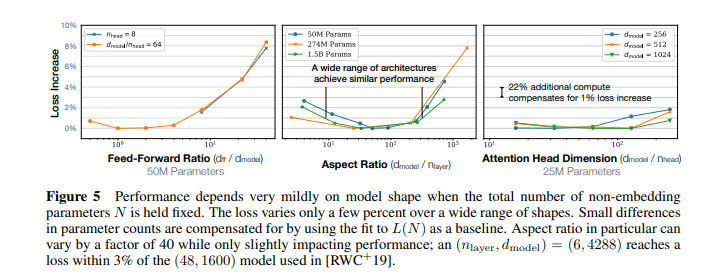
\includegraphics[width=0.9\textwidth]{./ffnn_scaling.png} % Adjust the width as needed
\end{figure}
\item \textbf{Generalization performance to other data distributions improves smoothly with model size}: A model trained on (for example) books and wikipedia generalizes between to datasets with other distributions (common crawl, webtext2, etc.) better and better as model size increases. 
\begin{figure}[H]
    \centering
    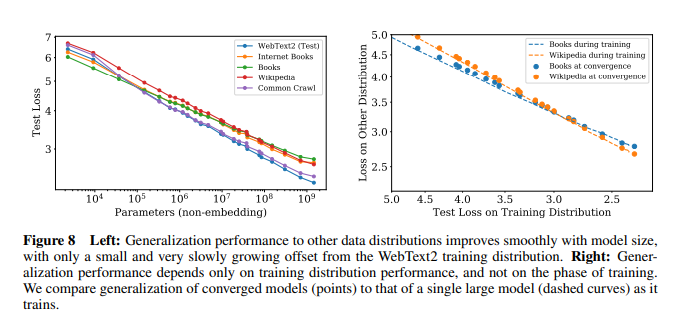
\includegraphics[width=0.9\textwidth]{./different_dists.png} % Adjust the width as needed
	\caption{Figure on the right shows that as test loss on training distribution decreases (it decreases as we increase model size) the model simultaneously becomes better at generalizing to other distributions (seems too good to be true, right?).}
\end{figure}
\end{itemize}

\section{Maximum FLOP Utilization}
Maximum FLOP Utilization (MFU) is a metric designed to estimate the efficiency of an LLM training accelerator. Previous metrics have focused on the ratio of FLOPs (Floating Point Operations) observed on a given device to its theoretical peak FLOPs. This is problematic because we may not care about doing as many FLOPs as we can but rather having high throughput (a high number of tokens processed per second). To do this, they compute:
\begin{enumerate}
    \item FLOPs per Token
    \item FLOPs per sample \(= \text{FLOPs per Token} \times \text{tokens per sample}\)
    \item FLOPs per iter \(= \text{FLOPs per Token} \times \text{tokens per sample}\)
    \item Useful FLOPs per Second \(= \frac{\text{FLOPs per iter}}{\Delta t}\), where \(\Delta t\) is the time it takes one iter to process
    \item MFU \(= \frac{\text{Useful FLOPs per Second}}{\text{Max Possible FLOPs per second (Per Hardware Specifications)}}\)
\end{enumerate}
This provides a substantially more accurate portrait of how efficient an LLM training architecture is. 

\section{Classical and Deep Reinforcement Learning Methods}
There are three fundamental kinds of RL algorithms:
\begin{enumerate}
\item Value Based Methods
\item Policy Based Methods
\item Actor Critic Methods (Kind of a hybrid of the other two)
\end{enumerate}
Below, I survey several of the most common and relevant examples of these algorithms.\\

\subsection{Policy Based Methods}
Policy based methods optimize the policy \(\pi\) directly by following the gradient of the expected reward with respect to the policy parameters \(\theta\):

\[J(\theta) = \mathbb{E}_{\tau \sim \pi_\theta}\left[\sum_{t=0}^Tr_t\right]\]
\begin{itemize}
\item \(\theta\) are the policy parameters. In Deep Reinforcement Learning,  this would be the literal weights of whatever neural network we're generating the policy (the decisions with). In classical RL, it would be some tabular set of values.
\item \(\tau\) is the trajectory. If we're training to play chess, it would the be sequence of all states \(s_t\), actions \(a_t\), and rewards \(r_t\) across a chess game. A single trajectory is an experience from initial state to terminal state. \(tau \sim \pi_\theta\) means the trajectory we take under policy \(\pi_\theta\).
\item \(r_t\) is the reward we receive at time \(t\).
\end{itemize}

We take the gradient of the policy with respect \(\theta\) and use gradient descent to backpropagate:
\[\theta \leftarrow \theta + \alpha \nabla_\theta J(\theta)\]

We calculate \( \nabla_\theta J(\theta)\) using the policy gradient theorem:

\[\nabla_\theta J(\theta) = \mathbb{E}_{\pi_\theta}\left[\nabla_\theta \text{log}\pi_\theta(a_t | s_t) \cdot Q^\pi (s_t, a_t)\right]\]
\begin{itemize}
\item \(\mathbb{E}_{\pi_\theta}\) is the expectation under the policy \(\pi_\theta\)
\item \(\nabla_\theta\) is the gradient with respect to our policy generator (neural net)
\end{itemize}
\subsubsection{REINFORCE}
REINFORCE is a simple Monte Carlo Policy Gradient method. It optimizes the policy directly by literally just backpropagating the derivative of our expected cumulative returns:
\[J(\theta) = \mathbb{E}_{\tau \sim \pi_\theta}\left[\sum_{t=0}^Tr_t\right]\]
\[\theta \leftarrow \theta + \alpha \nabla_\theta \text{log}\pi_\theta (a_t | s_t)G_t\]

Where \(G_t = \sum_{t=0}^Tr_t\). You might say, "why does this actually work? Surely the reward signal is profoundly muddy and you need huge numbers of iterations to get any kind of intelligent policy learned." You're absolutely right.  This is a very high-variance RL method that requires lots of iteration and careful tuning of hyperparameters in the policy generator.
\subsubsection{Proximal Policy Optimization (PPO)}
Proximal policy optimization is an on-policy RL algorithm designed to strike a blance between exploration and exploitation while also maintaining stability during training. It improves the policy iteratively by maximizing a cilpped surrogate objective, which ensures that updates don't deviate too far from the current policy:\\

Let \(\pi_\theta(a|s)\) be a policy parameterized by \(\theta\), outputting the probability of taking action \(a\) in state \(s\). Let \(A_t\) be the advantage function at timestep \(t\), representing how much better or worse \(a_t\) is than \(a_{t-1}\). The PPO objective is then:

\[\mathcal{L}^{\text{CLIP}}(\theta): \mathbb{E}\left[\min (r_t(\theta)A_t, \text{clip}(r_t(\theta), 1 - \epsilon, 1+\epsilon)A_t)\right]\]

Where \(r_t\) is the probability ratio between the new policy and the old policy:
\[r_t = \frac{\pi_\theta(a|s)}{\pi_{\theta_{\text{OLD}}}(a|s)}\]
Basically this insures 
\begin{itemize}
\item In the event of a positive reward \(A_t > 0\), it will clip the policy ratio \(r_t\) to ensure it doesn't jump too drastically (more conservative option)
\item In the event of a negative reward \(A_t < 0\), it will \emph{not} clip \(r_t\), so if \(r_t > 1\) (after update it is more likely to select bad option) the left side will be more negative. meanwhile if \(r_t \approx 0\) it \emph{will} clip \(r_t\), so there will be a negative gradient even if \(r_t \approx 0\). so in this case it picks the more extreme option always).
\end{itemize}

So basically it ensures the we proceed at a measured pace when the model does well, and strongly corrects when the model does poorly. This is called trust region optimization. \\

We then update the parameters using the policy gradient: 

\[\theta \leftarrow \theta + \alpha \nabla_\theta\mathcal{L}^{\text{CLIP}}(\theta)\]

Because PPO is on-policy (the model actually takes the actions it believes are best) it must rely on on-policy sampling balancing exploration and exploitation. This typically is done wtih some kind of stochastic sampling method that is still on-policy, while ensuring intrinsic exploration. The gradient of this function with respect to \(\theta\) is 

\[\nabla_\theta \mathcal{L}^{\text{CLIP}}(\theta) =  \mathbb{E} \left[ \nabla_\theta \text{log}\pi_\theta(a|s) \cdot \min (r_t(\theta)A_t, \text{clip}(r_t(\theta), 1 - \epsilon, 1+\epsilon)A_t)\right]\]

Which simplifies to 0 if outside the clipping range (because the probability ratio is outisde the clipping range, \(\mathcal{L}^{\text{CLIP}}(\theta)\) is constant. Inside the clipping range it is 

\[\nabla_\theta \mathcal{L}^{\text{CLIP}}(\theta) = r_t(\theta)A_t  \nabla_\theta \text{log}\pi_\theta(a|s) \]

Note that \(r_t(\theta)\) is outisde the gradient because 
\[r_t = \frac{\pi_\theta(a|s)}{\pi_{\theta_{\text{OLD}}}(a|s)}\]
\(\pi_{\theta_{\text{OLD}}}(a|s)\) does not depend on \(\theta\), but \(\pi_\theta(a|s)\) \emph{does} depend on \(\theta\). When we take the derivative wtih respect to \(\theta\) we use the log-derivative trick to get 
\[\nabla_\theta(r_t(\theta)A_t) = A_t \cdot r_t(\theta)\nabla_\theta \text{log}\pi_\theta(a_t|s_t)\]
So we do take the derivative with respect to \(r_t\) when calculating the gradient of the objective function, but because of the log derivative function we don't have to differentiate \(r_t\) directly.

\textbf{Question}: How does this actually balance the tradeoff between exploration and exploitation? \\

\textbf{Answer}: PPO doesn't expliclty include any kind of exploration policy like epsilon greedy exploration. Trust region optimization algorithms like this one, which ensure updates on model parameters don't deviate too far from the current policy, are vulnerable to converging to local optima, especially in the case of sparse reward signals. I imagine the key is to carefully fine-tune the hyperparameters in post training to make sure the reward signal won't encourage the model to prematurely converge, and to monitor training carefully to make sure it doesn't converge to local maxima. Also, here are a few things that help with avoiding local maxima:\\

\begin{enumerate}
\item Entropy Regularization (see section below on that)
\item Clipping inherently discourages premature exploration by preventing the model from taking drastic, large policy updates that converge quickly to suboptimal solutions
\item GAE (don't have a section on this yet)...
\end{enumerate}

With entropy regularization involved, the gradient with respect to the loss function becomes:

\[
\nabla_\theta \mathcal{L}_{\text{CLIP}}(\theta) =  \mathbb{E} \left[ \nabla_\theta \text{log}\pi_\theta(a|s) \cdot \min (r_t(\theta)A_t, \text{clip}(r_t(\theta), 1 - \epsilon, 1+\epsilon)A_t) + \beta \nabla_\theta H(\pi_\theta(\cdot \mid s))\right]
\]
Where
\[\nabla_\theta H(\pi_\theta(\cdot \mid s))  =  -\sum_{a \in A} (\pi_\theta(a|s)\text{log}\pi_\theta(a|s) + \pi_\theta(a|s)\nabla_\theta \text{log} \pi_\theta (a|s))\]
And \(\beta \in [0,1]\) is a hyperparameter controlling how exploration / exploitation should be balanced. Higher \(\beta\) means more exploration. Details of this derivation are below in entropy regularization section. As noted below, the objective function is something we want to maximize in RL algortihms, and that means it will be pushed towards policies with higher entropy.

\subsection{Actor-Critic (Advantage Actor Critic)}
Actor-Critic Methods combnie policy-based and value-based RL approaches. The idea is to use a value based "Critic" to reduce the variance of policy gradient updates while still using the policy (Actor) to make decisions:
\begin{itemize}
\item \textbf{Actor}: policy \(\pi_\theta(a|s)\) parameterized by \(\theta\) selects actions based on the state
\item \textbf{Critic}: the value function \(V_\phi(s)\), parameterized by \(\phi\), estimates the expected return from state \(s\).
\end{itemize}
\textbf{Classical Actor Critic} learns a critic model \(V(s)\) using the temporal difference error \(\delta\):
\[V(s) \leftarrow V(s) + \alpha_\text{critic}\cdot \delta\]
\[\delta = r + \gamma V(s') - V(s)\]

And a critic model \(\pi(s,a)\) with this update equation:
\[\pi(s,a) \leftarrow \pi(s,a) + \alpha_\text{actor}\cdot A(s,a)\]
Where the advantage estimate \(A(s,a) = r -V(s)\) 

As a quick example, let's say we have some dummy critic that outputs \(V(s)=0.5\) for all \(s\). Let's say \(\gamma=0.4\) and \(\alpha=0.1\) and we reach a reward state where \(r=1\). How would this update work?
\[\delta \leftarrow 1 + (0.4)\cdot(0.5) - 0.5 =1 - 0.2 - 0.5 = 0.3\]
Then 
\[V'(s) \leftarrow 0.5 + (0.1)\cdot(0.3) = 0.5 + 0.03 = 0.53\]
Gradually, it would learn to better estimate the true value of state \(s\).\\

\textbf{Deep Actor Critic} uses deep neural networks as both the actor and critic. The formulas are similar, but I thought I'd give a more intelligible introduction here up above. \\

The actor is  trained using the log-probability of it selecting move \(a\) in state \(s\) \(\times\) the Advantage function, which estimates the advantage gained by making action \(a\) using the critic:
\[\nabla_\theta \mathcal{L}_\text{actor} = \nabla_\theta \log \pi_\theta(a|s) \cdot A(s,a)\]
\(\log \pi_\theta(a|s)\) is the log-probability of the actor taking action a in state s under policy \(\pi_\theta\). \\

\textbf{Question}:  let's say the agent has a probabiltiy of taking the action a = 1 (so it always does this), but action s is wrong. log(1) = 0, so wouldn't the agent never learn to not take action a in state s?\\

\textbf{Answer}: Yes. But everyone in the universe will use the softmax function to convert the logits output by \(\theta\) into probabilities, and this will prevent it from ever reaching \(p(a|s) = 1\).\\

The advantage function is given by 

\[A(s,a) = r + \gamma V(s') - V(s)\]

Where \(V(s)\) is our critic. Let's say its a neural network with parameters \(\theta_v\). The critic learns with this gradient update rule:
\[\nabla_{\theta_v}\mathcal{L}_\text{critic} = \nabla_{\theta_v}(r + \gamma V(s'; \theta_v) - V(s; \theta_v))^2\]
So it's just the squared temporal difference error.

\section{Policy Gradient Theorem}
The policy gradient theorem provides us a method to compute the gradient of the expected cumulative return \(J(\theta)\) of a reward function with respect to some policy generator \(\theta\) without having to differentiate the reward function itself:\\ 


Let's our objective function is the sum of expected rewards across some trajectory \(\tau\) under policy \(\pi_\theta\):
\[J(\theta) = \mathbb{E}_{\tau \sim \pi_\theta}\left[\sum_{t=0}^Tr_t\right]\]
We want to take the derivative with respect to our policy generator \(\theta\) to optimize it:
\[\nabla_\theta J(\theta) =\nabla_\theta \mathbb{E}_{\tau \sim \pi_\theta}\left[\sum_{t=0}^Tr_t\right]\]
Because the expectation of the derivative is the derivative of the expectation, we can write:
\[\nabla_\theta J(\theta) = \mathbb{E}_{\tau \sim \pi_\theta}\left[\nabla_\theta \text{log}\pi_\theta (\tau)\sum_{t=0}^Tr_t\right]\]
Where \(\text{log}\pi_\theta (\tau)\) is the log-probability of taking trajectory \(\tau\) under policy \(\pi_\theta\). We can add this in here because of the \textbf{log-derivative trick} (see section on the log derivative trick for explanation. Now we don't need to differentiate the reward function).\\

Next, we recognize that 

\[\text{log}\pi_\theta (\tau) = \sum_{t=0}^\tau \text{log} \pi_\theta (a_t | s_t)\]

Which gives us our formula for the gradient in which we don't have to worry about differentiating the reward function \(r_t\):

\[\nabla_\theta J(\theta) =\mathbb{E}_{\tau \sim \pi_\theta}\left[\sum_{t=0}^T \nabla_\theta \text{log} \pi_\theta (a_t | s_t) \cdot \sum_{t=0}^T \text{log} r_t\right]\]

\section{Entropy Regularization}:
Entropy regularization is a technique used in reinforcement learning to encourage exploration by adding an entropy term to the optimization objective. For some policy \(\pi_\theta(a|s)\) (imgine a LLM is this policy, and \(\pi\) are its weights), the entropy is:

\[H(\pi_\theta(\cdot|s)) = -\sum_{a\in A}\pi_\theta(a|s)\log \pi_\theta(a|s)\]
So the idea is that if there is a single action \(a\in A\) where \(\pi_\theta(a|s) \rightarrow 1\), then  \(H(\pi_\theta(\cdot|s)) \rightarrow 0\) because of this logarithm property:
\[\text{lim}_{x \rightarrow 0} x\log x = 0\]
With no entropy regularization, the objective function we seek to maximize (the expected cumulative rewards over a given rollout \(\tau\)) is:
\[
J(\theta) = \mathbb{E}_{\tau \sim \pi_\theta}\left[\sum_{t=0}^{\tau} r_t\right]
\]
With entropy regularization, this becomes:
\[
J(\theta) = \mathbb{E}_{\tau \sim \pi_\theta}\left[\sum_{t=0}^{\tau} r_t + \beta H(\pi_\theta(\cdot \mid s)) \right]
\]

where \(\beta > 0\) is a hyperparameter controlling the trade-off between exploration (higher entropy means more exploration) and exploitation (lower entropy means greater reward maximization and more exploitation). The gradient of this whole function with respect to the weights \(\theta\) is calculated with the policy gradient theorem:
\[\nabla_\theta J(\theta) = \mathbb{E}_{\tau \sim \pi_\theta}\left[\nabla_\theta \text{log}\pi_\theta (\tau)\sum_{t=0}^\tau  r_t + \nabla_\theta \beta H(\pi_\theta(\cdot \mid s))\right]\]
Where
\[ \nabla_\theta \beta H(\pi_\theta(\cdot \mid s)) = -\sum_{a \in A} (\pi_\theta(a|s)\text{log}\pi_\theta(a|s) + \pi_\theta(a|s)\nabla_\theta \text{log} \pi_\theta (a|s))\]
By the product rule. This term gets larger as entropy increases, and since we're trying to \emph{maximize} the objective function, the model is therefore encouraged to explore. 
\section{Variational Autoencoders}
A Variational Autoencoder (VAE) is a deep generative neural network which maps some input image (I'm going to pretend we're working on images here, but it doesn't have to be an image) to a \textbf{probability distribution}  in an n-dimensional latent space. Then, we sample from that distribution at inference time to generate new images.\\
\subsection{Training}
A VAE consists of an encoder and a decoder. In training, we want to make sure the encoder learns the latent space distribution \((\theta = \mu, \log(\sigma^2))\) of the input \(x\) that maximizes the likelihood of observing \(x\) given our chosen distribution:
\[\max_\theta(p_\theta(x) = p(x | \theta))\]

Meanwhile, we want to make sure the decoder learns to recreate the original image from the latent distribution (note the presence of noise in this image--this makes it a distribution rather than simply latent variables):

\[z = \mu + \sigma \odot \epsilon, \quad \epsilon \in N(0,1)\]

The loss function reflects the fact that our encoder and decoder perform distinct roles and must both be optimized:

\[\mathcal{L}_{VAE}= \mathbb{E}_{q(z|x)}[\log(p(x|z))] - D_{KL}(q(z|x)||p(z))\]

The first loss term is the reconstruction loss. The 2nd is the KL-Divergence. The KL divergence (see section on KL divergence) is essentially a regularization term that penalizes the encoder for deviating from the prior distribution (which is typically set to be the standard normal gaussian. So the further \((\theta = \mu, \log(\sigma^2))\) differs from the standard normal parameters, the larger this term gets.\\

The first term is the reconstruction loss. This loss measures how well the reconstructed data matches the original input data. The reconstruction loss obviously trains the decoder, but it also trains the encoder because the quality of the laten space representations z provided by the encoder influences how well the decoder can reconstruct the image. \\

While the expectation of the log likelihood ratio might look intimidating, it is typically computed either as Mean Squared Error or (for binary or normalized data, pixel values between 0 and 1) as binary crossentropy loss. Why is this allowed? In the equation above the first term is the log likelihood of a gaussian distribution:

\[ \mathbb{E}_{q(z|x)}[\log(p(x|z))] \]

The log likelihood of a gaussian distribution evaluates to 

\[ \mathbb{E}_{q(z|x)}[\log(p(x|z))] = -\frac{1}{2\sigma^2}|| x - \hat{x}||^2\]

Maximizing the log likelihood of a Gaussian distribution means finding the value of z that minimizes this (to understand why, see my section on Maximum Likelihood Estimation in the Estimation Theory Fundamentals section). \\

Meanwhile, if we assume the data x given z follows a Bernouli Distribution (suitable for binary or normalized data), maximizing \(\log(p(x|z))\) is equivalent to minimizing the Binary Crossentropy Loss. Pretty cool.
\section{R1 \& Group Relative Policy Optimization (Advanced ML Concept)}
DeepSeek's R1 algorithm is an open-source, open-weight LLM that matched many of the capabilities of the most advanced frontier LLMs in January 2025. It uses a fairly standard large-scale pretraining process, paired with \emph{Unsupervised} Group Relative Policy Optimization reinforcement learning and chain-of-thought prompting to achieve SOTA performance in math and coding capabilities. Here I will review the paper's algorithms. \\

\subsection{Group Relative Policy Optimization}
Group relative policy optimization is an online, on-policy RL algorithm very similar to Proximal Policy Optimization. In fact, the only real differences between the two are:

\begin{enumerate}
\item The objective function \(\mathcal{J}(\theta)\) in PPO maximizes expected cumulative reward over a rollout from time \(t=0 \rightarrow \tau\). In GRPO, we maximize expected cumulative reward over \(G\) sampled outputs to the same question \(q\). 
\item Rather than doing entropy regularization explicitly as we might in PPO, GRPO uses a KL-Divergence term to explicitly penalize the model from drifting too far from the original policy, even if it occurs gradually, while also implicitly preserving exploration, because we assume that \(\pi_\text{ref}\) is already optimized to generate diverse responses. 
\item The Advantage function captures the relative performance within a group, rather than performance relative to \emph{all training samples}. This means that we explicitly get more stable learning, because total advantages across all minibatches in a given group will be constant. And it also means we get better context-specific rewards which lead to better local exploration and enhanced policy diversity.
\end{enumerate}

The full equation for GRPO is:

\noindent
\resizebox{1.4\linewidth}{!}{%
$
\mathcal{J}(\theta) = \mathbb{E}_{q \sim P(Q), \{o_i\}_{i=1}^{G} \sim \pi_{\text{old}}(O|q)}
\left[
\frac{1}{G} \sum_{i=1}^{G}
\min \left(
\frac{\pi_\theta(o_i | q)}{\pi_{\theta_{\text{old}}}(o_i | q)} A_i, 
\text{clip}\left(\frac{\pi_\theta(o_i | q)}{\pi_{\theta_{\text{old}}}(o_i | q)}, 1 - \epsilon, 1 + \epsilon\right) A_i
\right) 
- \beta \mathbb{D}_{\text{KL}}(\pi_{\theta} \| \pi_{\text{ref}})
\right]
$
}

Again, notice the similarities between this and PPO. Literally the only three differences are the three listed above. 

The KL divergence equation used in GRPO is:

\[
\mathbb{D}_{\text{KL}}(\pi_{\theta} \| \pi_{\text{ref}}) = 
\frac{\pi_{\text{ref}}(o_i | q)}{\pi_{\theta}(o_i | q)} - \log \frac{\pi_{\text{ref}}(o_i | q)}{\pi_{\theta}(o_i | q)} - 1
\]

And the advantage function is:

\[
A_i = \frac{r_i - \text{mean}(\{r_1, r_2, \dots, r_G\})}{\text{std}(\{r_1, r_2, \dots, r_G\})}
\]

Note that if we were only doing one gradient update per group, then the advantage function \(A\) would effectively be constant. Instead, we typically do multiple minibatch gradient updates in a single group.


\subsection{Chain-of-Thought Prompting}
Chain of Thought Prompting is a method which encourages LLMs to "think harder" about more challenging problems by prompting them to encode their reasoning process (chain of thought) and their final answer in their response. They are told to output their reasoining process within \texttt{<think><think>} tags and their answer, which must come after, in \texttt{<answer><answer>} tags. The result is that the LLM will not terminate its chain of thought until it arrives at some reasonable answer, and thus will devote more tokens in their response (and more compute resources) to problems which have a more challenging answer. This has been shown to substantially improve model reasoning capability on complicated problems by resolving the fixed-compute-per-output-token problem, which many believed was a foundational limitation of LLMs that necessitated the development of fundamentally different architectures in order to achieve advanced machine intelligence. Here's an example of a chain-of-thought prompt from the DeepSeek Paper:

\subsection{Reward Signal}
Typically the reward signal comes from human data (RLHF) to align the model's usability with the way humans expect to interact with it. But here we use \emph{Accuracy Rewards} (was the model's final answer/code correct) and \emph{Forma Rewards} (did the model correctly adhere to the format provided in the prompt. These rewards are both automated and therefore are unsupervised. This is a major improvement that, coupled iwth the emergent behavior observed when utilizing chain-of-though prompting and ultralong context length inputs that are now possible thanks to things like Ring Attention, mean there is a very very high upper bound on LLM performance. 


\begin{figure}[H]
    \centering
    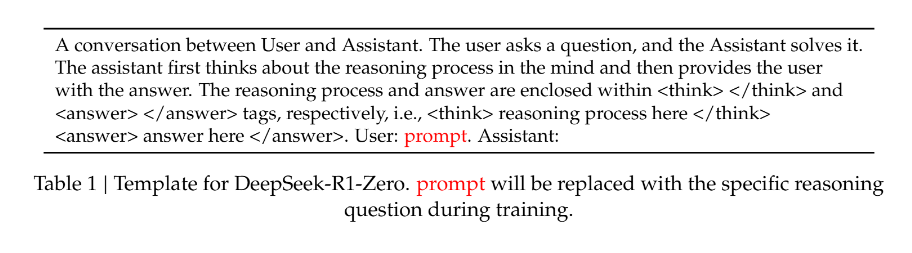
\includegraphics[width=0.8\textwidth]{./deepseekcot.png} % Adjust the width as needed
\caption{An example of a chain-of-thought prompt}
\end{figure}

So, the full process / big picture is this:
\begin{itemize}
\item Pretrain the model normally (with chain-of-thought prompting)
\item Use GRPO to fine-tune the model on tasks like coding and math. 
\item with chain of thought prompting, behavior will naturally emerge in which the model devotes more output tokens to challenging problems, and also a dramatic increase in reasoning ability. 
\begin{figure}[H]
    \centering
    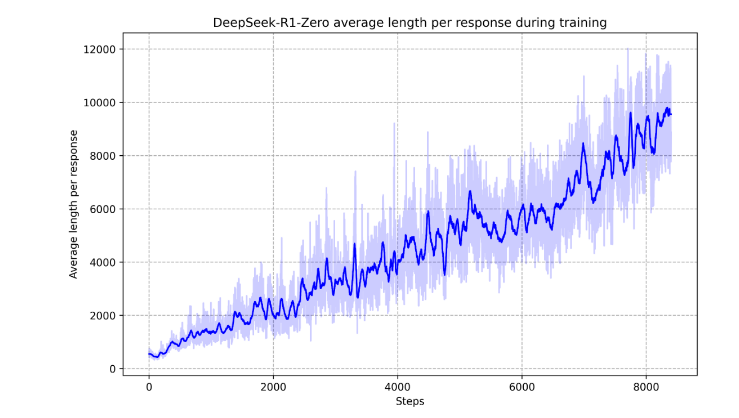
\includegraphics[width=1.0\textwidth]{./deepseekresponse.png} % Adjust the width as needed
\caption{As training progresses, we observe an increase in response length alongside an increase in reasoning ability and problem solving accuracy}
\end{figure}
\end{itemize}

\section{Multivariate Gaussians}

The formula for the multivariate gaussian is for \(k\) variables given by 
\[f(\underbar{x}; [\mu, \Sigma]) = \frac{1}{(w\pi)^{\frac{k}{2}}det(\Sigma)}e^{-\frac{1}{2}(\underbar{x} - \mu)^T \Sigma^{-1}(\underbar{x} - \mu)}\]

\(\mu\) is a \(n \times 1\) vector of the means of each of the \(n\) variables comprising the gaussian:

\[\mu = \left[ \begin{array}{c} \mu_1 \\ \mu_2 \\ \vdots \\ \mu_n \end{array}\right]\]

\(\Sigma\) is the Covariance Matrix:
The Covariance matrix expresses the covariance (correlation) between each pair of features. for features \(Z_1\) and \(Z_2\), their covariance is given by \[Cov(Z_1,Z_2) = \frac{1}{M-1} \sum_{i \in M} (Z_{1,i} - \mu_{Z_1})(Z_{2,i} - \mu_{Z_2})\]
where M is the number of features. This would be a single entry in the covariance matrix:
\[ \Sigma = 
\left[
\begin{array}{cccc}
\text{Var}(Z_1) & \text{Cov}(Z_1, Z_2) & \cdots & \text{Cov}(Z_1, Z_m) \\
\text{Cov}(Z_2, Z_1) & \text{Var}(Z_2) & \cdots & \text{Cov}(Z_2, Z_m) \\
\vdots & \vdots & \ddots & \vdots \\
\text{Cov}(Z_m, Z_1) & \text{Cov}(Z_m, Z_2) & \cdots & \text{Var}(Z_m) \\
\end{array}
\right]
\]

The covariance matrix for a dataset with m features is an \( m \times m \) matrix where each element \((Z_i,Z_j)\) represents the covariance between  \(Z_i\) and \(Z_j\)  

Note that \( \Sigma^{-1}\) denotes the inverse of the covariance matrix \(\Sigma\) and \(det(\Sigma) = ad - bc\) for a \(2 \times 2\) matrix (bivariate gaussian) Why does using the determinant here make sense? Consider this: the joint PDF of two jointly gaussian independent random variables \(x\) and \(y\) is just the product of the two individual pdfs. This means that the magnitude term (the fraction out in front of the exponential term, which ensures the PDF integrates to 1) is:

\[\frac{1}{2\pi \sigma_x \sigma_y}\]

If  \(x\) and \(y\) are independent, then \(det(\Sigma) = \sigma_x \sigma_y - 0\) and our magnitude term is the same. If they aren't independent, then the determinant properly accounts for their relationship in the magnitude term.  

Another interesting piece of intuition is this: the determinant (in 2D) is a measure of the area of the column vectors that compose the matrix. So you can actually use \(det([a,b])\) to calculate the area of a paralellogram whose sides are the vectors \(a\) and \(b\). And in 3d the determinant measures the volume of a paralellogram, and so on. So what we're really doing here is normalizing by dividing by the volume of the n-dimensional hyper-parallelogram whose sides' lengths are defined by the column vectors in \(\Sigma\). 

\section{Regularization}

Regularization is a technique used in machine learning and statistics to prevent overfitting by imposing penalties on the size of the coefficients, ensuring simpler models that generalize better to unseen data.

\subsection{Mathematical Explanation}

Regularization involves adding a penalty term to the objective function being minimized by the learning algorithm. This penalty term constrains the magnitude of the model parameters, focusing the model on the most significant features. The most common regularization techniques are:

\begin{itemize}
    \item \textbf{L1 Regularization (Lasso):} Incorporates the sum of the absolute values of the coefficients into the loss function, leading to sparse solutions.
    \[ \text{Loss Function} = \text{Original Loss} + \lambda \sum_{i=1}^{n} |w_i| \]
	\item \textbf{Sparsity}: Sparsity is when the weights of the model are all nearly zero. 
    
    \item \textbf{L2 Regularization (Ridge):} Adds the sum of the squares of the coefficients to the loss function, distributing the penalty among all features.
    \[ \text{Loss Function} = \text{Original Loss} + \lambda \sum_{i=1}^{n} w_i^2 \]
\end{itemize}

\textbf{Why does L1 regularization encourage sparsity more than L2?} Because \(|w_i| > w_i^2 \ \forall w_i < 1,\) it follows that \( \mathcal{L}_{L1} > \mathcal{L}_{L2} \ \forall w_i < 1\). Since the weights of a neural net are nearly always less than 1, this means that L1 loss effectively penalizes weights creeping upward more than L2 loss. Both regularization losses encourage sparsity, obviously, but given the typical range of weights in neural nets, L1 loss encourages it more. 

\subsection{Why It Works}

Regularization reduces overfitting by introducing a bias that lowers variance, following the bias-variance trade-off. By penalizing large coefficients, it ensures the model captures only the most significant patterns, enhancing predictive power on unseen data.

Adding in this term to the loss will penalize larger weights and encourage them to stay as close to zero as possible. It does this because when we take the gradient of the loss function, the negative gradient of the 2nd term will point towards zero, thus biasing the weights to be smaller.

\subsubsection{Example of L2 Regularization Effect on Weight Update}

Consider a simple scenario where we focus solely on the regularization term, assuming the original loss component is zero for simplicity. Let's examine how L2 regularization affects the weights through gradient descent.

Given model weights \(w_1 = -1\) and \(w_2 = 2\), and a regularization strength \(\lambda = 0.1\), the L2 regularization term is:

\[ L_{reg} = \lambda \sum_{i=1}^{n} w_i^2 \]

The gradient of \(L_{reg}\) with respect to each weight \(w_i\) is:

\[ \frac{\partial L_{reg}}{\partial w_i} = 2\lambda w_i \]

For our weights, this yields:

\begin{itemize}
    \item For \(w_1 = -1\): \(\frac{\partial L_{reg}}{\partial w_1} = 2 \cdot 0.1 \cdot (-1) = -0.2\)
    \item For \(w_2 = 2\): \(\frac{\partial L_{reg}}{\partial w_2} = 2 \cdot 0.1 \cdot 2 = 0.4\)
\end{itemize}

Assuming a learning rate \(\eta = 1\) for simplicity and ignoring the rest of the loss function, the weight update rule becomes \(w_i = w_i - \eta \cdot \frac{\partial L_{reg}}{\partial w_i}\) (remember that we're ignoring the rest of the loss aside from \(L_{reg}\)):

\begin{itemize}
    \item New \(w_1 = -1 - (-0.2) = -0.8\)
    \item New \(w_2 = 2 - 0.4 = 1.6\)
\end{itemize}

This example demonstrates how the L2 regularization term's gradient, pointing towards zero, effectively shrinks the weights \(w_1\) and \(w_2\) towards zero during the update step. The magnitude of this effect is controlled by the regularization parameter \(\lambda\), balancing the impact of regularization against the original loss function.


\subsection{When to Use}

\begin{itemize}
    \item In scenarios indicative of overfitting, where model performance on training data significantly surpasses performance on validation/test data.
    \item With high-dimensional data, where the number of features greatly exceeds the number of observations.
    \item For feature selection purposes, particularly with L1 regularization which can zero out some coefficients.
    \item To improve model interpretability by simplifying its complexity through parameter magnitude constraints.
\end{itemize}

Regularization is a cornerstone in building robust and interpretable machine learning models, balancing complexity against the capacity to generalize across different datasets.

\section{Trimmed Mean}

The trimmed mean, also known as the truncated mean, is a statistical measure designed to calculate the average of a dataset by excluding a specified percentage of the lowest and highest values, thereby reducing the influence of outliers.

\subsection{How It Works}

\begin{enumerate}
    \item \textbf{Specify Trim Percentage}: Determine the percentage of data points to remove from both the lower and upper ends of the dataset.
    \item \textbf{Sort the Data}: Organize the data points in ascending order.
    \item \textbf{Trim the Data}: Exclude the determined percentage of data points from both extremes of the dataset.
    \item \textbf{Calculate the Mean}: Compute the arithmetic mean of the remaining data.
\end{enumerate}

\subsection{Usefulness}

The trimmed mean offers robustness against outliers and extreme values, making it a more reliable measure of central tendency, particularly in skewed distributions. It strikes a balance between the comprehensive nature of the arithmetic mean and the outlier resistance of the median.

\subsection{Differences from Arithmetic Mean}

Unlike the arithmetic mean, which includes all values in its calculation, the trimmed mean excludes extreme values from both ends of the dataset, thereby providing a safeguard against the influence of outliers and significantly skewed data.

\subsection{When to Use It}

\begin{itemize}
    \item In datasets expected to contain outliers or extreme values.
    \item For analyzing skewed data where an untrimmed mean might not accurately represent the central tendency.
    \item When comparing central tendencies across datasets with different levels of skewness or outlier presence, providing a consistent and robust measure.
\end{itemize}
\section{Bayes' Theorem}
Bayes' Theorem is a mathematical rule for inverting conditional probabilities. Given two random variables \(A\) and \(B\):

\[P(A|B) = \frac{P(B|A)\cdot P(A)}{P(B)}\]

\subsection{Proof}
Start with the definition of conditional probability for both \(A\) and \(B\):
\[P(A|B) = \frac{P(A \land B)}{P(B)}\]
\[P(B|A) = \frac{P(A \land B)}{P(A)}\]
solve the bottom equation for \(P(A \land B)\):
\[P(A \land B) = P(B|A)P(A)\]
Now substitute this into the top equation and we have Bayes' Theorem:

\[P(A|B) = \frac{P(B|A)\cdot P(A)}{P(B)}\]

\section{Style Transfer}
Style Transfer is a class of problems in image processing that involve the application of the stylistic characteristics of one image (the style reference) to the content of another (the content target), resulting in a new image that retains the content of the target but exhibits the artistic style of the reference. Mathematically, style transfer can be formulated as an optimization problem:

Given a content image \(c \in X\) and a style image \(s \in Y\), where \(X\) and \(Y\) represent the domains of content and style images respectively, we seek to learn a mapping \[f(c \in X) \rightarrow g \in Y\] 

Such that \(f(x)\) minimizes the high-level content difference between \(f(x)\) and \(c\), as well as the lower-level style difference between \(f(x)\) and \(s\).

There are a number of different machine learning techiniques, three of which are covered belolow, Neural Style Transfer, GANs (specifically CycleGAN) and Diffusion Models

\section{Neural Style Transfer (Gatys et al.)}

The original style transfer algorithm by Gatys et al. achieves style transfer 
by synthesizing a new image \(g = f(c)\) retaining the content of image \(c \in X\) while adopting the style of the style image \(s \in Y\). 

Gatys et al. used two loss functions, \(L_{content}\) and \(L_{style}\), which measure the difference in content between generated image \(g\) and content image \(c\), and the difference in style between generated image \(g\) and style image \(s\).

The generated image \(g\) and the original image \(c\) are both iteratively passed through some pretrained neural network (such as VGGNet), which is used as a feature extractor. \(g\) is initialized either as random noise or as an exact copy of the content image \(c\). The content features are pulled one or more layers that are deep enough in the network to capture high level content features (the shallowest layers focus on basic features like edges), but not so deep that they are insensitive to the exact appearance of features in the image. The outputs from the sampled layers are fed through our first loss function \(L_{content}\) like this:

\begin{equation}
    L_{content}(C, G) = \frac{1}{2} \sum_{i, j} \left( F^l_{ij}(G) - F^l_{ij}(C) \right)^2
\end{equation}

Where \(l\) represents the \(l^{th}\) layer in the network (we may choose one or more layers to sample from), and \(F^l_{ij}(G)\) is the activation of the \(i^{th}\) filter at position \(j\) in layer \(l\).

The style loss is generated by sampling multiple layers throughout the network. Earlier layers are sampled to capture basic textures and colors, and deeper layers are also sampled to capture more complex patterns. The 'style' is captured by calculating the Gram matrix for each layer, which can conceptually be thought of as the covariance matrix for the feature maps for a given layer \(l\):

\begin{equation}
    E_l = \frac{1}{4N_l^2M_l^2} \sum_{i, j} \left( G^l_{ij}(G) - G^l_{ij}(S) \right)^2
\end{equation}

\subsection{Gram Matrices}
\subsubsection{What is a Gram Matrix?}
A Gram matrix is simply a mathematical concept used to represent the inner products between different sets of vectors. Given a set of vectors \(V = \{v_1, v_2, ..., v_n\}\), the Gram matrix \(G\) of \(V\) is just a matrix where each element \(G_{ij}\) is the inner product of the vectors \(v_i\) and \(v_j\):
\[G_{ij} = \langle v_i, v_j \rangle \]
In neural networks, especially convolutional neural networks used for image processing, the vectors \(v_i\) can be the flattened version of the feature maps (filters) activations at a certain layer. If we have a set of  \(N\) feature maps each of size \(M\) (after flattening), then our set \(V\) will have \(N\) vectors each of length M, and the Gram matrix will be of size \(N \times N\). Note that this is \(N \times N\), not \(N \times M\)! This is because the inner product of two vectors of length \(M\) is a single scalar value.
\subsubsection{Why does this work?}
It seems like it shouldn't work, but the reason it does is that the Gram matrix is very similar to a covariance matrix (it's actually literally the same thing except the features are vectors). By forcing the generated image's Gram matrix to approximate that of the style image (and that is what you're doing), you're indirectly forcing the patterns present at the sampled layers to match (you're forcing the features in the different layers to correlate in the same way). This, coupled with the fact that you're sampling layers throughout the network (so focusing on correlation rather than raw MSE, and also focusing on different, and more, layers) is responsible for capturing the style of one image.  Meanwhile, the content step ensures that the literal images match in broad strokes (it takes the MSE directly on the features themselves, rather than correlating them with a gram matrix and then taking the froebenius norm (which is similar to MSE). Hopefully that makes sense.\\

The weighted sum of \(E_l\) across all sampled layers gives the style loss:

\begin{equation}
    L_{style}(S, G) = \sum_{l} w_l E_l
\end{equation}

The total loss for our network is given by:
\begin{equation}
L_{total}(C,S,G) = \alpha L_{style}(S, G) + \beta L_{content}(C, G)
\end{equation}
As we iterate, generated image's pixel values are directly modified to reduce the total loss, making the image more stylistically similar to the style image while preserving the content of the content image. 

\section{CycleGAN (Zhu et al.)}

CycleGAN by Zhu et al. accomplishes style transfer via a Generative Adversarial Network (GAN), which enables the network to learn with unpaired data. The basic GAN consists of two neural nets, a generator \(G\) and a Discriminator \(D\). They compete with one another; \(D\) attempts to discriminate between real and fake images, while \(G\) attempts to generate images that are realistic enough to 'fool' \(D\). This competition is enforced via an adversarial set of loss functions for \(G\) and \(D\):

\begin{equation}
L_D = -\frac{1}{2}\mathbb{E}_{x\sim p_{data}(x)}[\log D(x)] - \frac{1}{2}\mathbb{E}_{z\sim p_z(z)}[\log(1 - D(G(z)))]
\end{equation}

\begin{equation}
L_G = -\frac{1}{2}\mathbb{E}_{z\sim p_z(z)}[\log D(G(z))]
\end{equation}

Where D(G(z)) = 0 means the Discriminator is completely certain a generated image is fake. While, D(G(z))=1 means it's completely fooled and believes a fake image is real. D(x) = 0 means it believes a real input image is real. \\

Here, \(L_D\) represents the loss function for the discriminator, which aims to maximize the probability of correctly classifying both real and fake images. \(L_G\) represents the loss function for the generator, which aims to minimize the probability that \(D\) correctly classifies fake images as fake.

The CycleGAN architecture consists of two generators, \(G: X \rightarrow Y\) and \(F: Y \rightarrow X\), and two discriminators, \(D_X\) and \(D_Y\), where \(D_X\) aims to distinguish between images \(x\) and translated images \(F(y)\), and \(D_Y\) aims to distinguish between images \(y\) and translated images \(G(x)\). 



A modification to the traditional GAN loss function enforces cycle consistency, a property which states that an image from a source domain \(X\), when translated to a target domain \(Y\) and back to \(X\), should retain its original content. Mathematically, this is expressed as:

\begin{equation}
G(F(x)) \approx x
\end{equation}
For \(x \in X\) and \(F: X \rightarrow Y, G: Y\rightarrow X\)

We can enforce cycle-consistency for both \(G: X \rightarrow Y\) and \(F: Y \rightarrow X\) by adding a term \(L_{cycle}\) to the traditional gan loss function. We define \(L_{cycle}\) as:
\[L_{cycle}(F) = \mathbb{E}_{x \sim p_{data}(x)}[\|F(G(x)) - x\|_1]\]
\[L_{cycle}(G) = \mathbb{E}_{y \sim p_{data}(y)}[\|G(F(y)) - y\|_1]\]

giving the total loss function:
\begin{equation}
L_{cycle}(G, F) = L_{cycle}(F) + L_{cycle}(G)
\end{equation}

We then add this term to the GAN loss function above. When we change the syntax to reflect the fact that we now have two sets of generators and discriminators, we get the following cycleGAN objective:

\begin{align}
    L(G, F, D_X, D_Y) = &L_{G: X \rightarrow Y}(G, D_Y, X, Y) \nonumber \\
    &+ L_{F: Y \rightarrow X}(F, D_X, Y, X) \nonumber \\
    &+ \lambda L_{cycle}(G, F)
\end{align}

Where \(L_{G: X \rightarrow Y}\) is the loss function associated with mapping \(X \rightarrow Y \) and is used to update G (the generator that transforms \( x \in X\) to \(y \in Y\)) and \(D_Y\) (the discriminator that attempts to discern images native to \(Y\) from generated images in domain \(Y\) \(L_{F: Y \rightarrow X}\) is the loss term for the generator and discriminator operating in the opposite direction. 

Cycle Consistency improves upon the traditional GAN paradigm by: 
\begin{itemize}
\item\textbf{Preventing Mode Collapse \& Improving Performance}: Cycle consistency ensures the network cannot simply output the same image in domain \(Y\) for every input \(x \in X\), because doing so would violate cycle consistency and lead to a higher loss. Just as important, it leads to richer and more variegated generative behavior.
\item\textbf{Enhancing Stability}: Cycle consistency effectively acts as a form of regularization, which makes the training process more stable and generalizeable. It also can improve the dynamics between generator and discriminator, which ensures a more stable training process.
\end{itemize}
\section{Diffusion Process}
A diffusion process is a stochastic differential equation that models the evolution of a system under a combination of random fluctuations and deterministic trends over time. A concrete example of how it is used in physics is to model the motion of particles suspended in a fluid. It is the mathematical foundation for diffusion models. Here we define how diffusion processes work in the context of a specific examle. Consider the motion of a dust particle in a room influenced by environmental factors such as air currents and random molecular collisions. We model this situation using a stochastic differential equation (SDE) in three-dimensional space.

Let \(X_t \in \mathbb{R}^3\) denote the position of the dust particle at time \(t\). The dynamics of \(X_t\) are described by the following SDE:
\[
dX_t = b(X_t, t) \, dt + \sigma(X_t, t) \, dW_t,
\]
where \(b(X_t, t)\) is the drift coefficient, \(\sigma(X_t, t)\) is the diffusion coefficient, and \(dW_t\) is the increment of a Wiener process.

\textbf{Drift Coefficient} \(b(X_t, t)\):
The drift coefficient \(b(X_t, t)\) models the deterministic part of the motion, which in this case might include the effect of air currents pushing the particle. For simplicity, let's assume \(V(x) = \frac{1}{2}k \|x\|^2\), where k is a constant that might represent the strength of the central air current pushing particles towards a specific point (like a vent, and in this definition the strength is greater the farther you go from the origin). This can be expressed as:
\[
b(X_t, t) = -\nabla V(X_t) = -k X_t,
\]
where \(k\) is a constant representing the strength of the air currents.

\textbf{Diffusion Coefficient} \(\sigma(X_t, t)\):
The diffusion term models random perturbations due to collisions with air molecules. It is often modeled as a constant:
\[
\sigma(X_t, t) = \sigma I,
\]
where \(\sigma\) is a scalar indicating the intensity of the random fluctuations, and \(I\) is the identity matrix in \(\mathbb{R}^{3 \times 3}\).

\textbf{Complete SDE}:
Combining these components, the full SDE is given by:
\[
dX_t = -k X_t \, dt + \sigma I \, dW_t,
\]
illustrating the particle's behavior under combined systematic and random influences.
\section{Wiener Processes (Brownian Motion)}

A Wiener process, also known as Brownian motion, is a fundamental continuous-time stochastic process. It is defined by the following properties:

\subsection{Construction of a Wiener Process}
One common way to construct a Wiener process is via the Donsker's theorem or the invariance principle. Consider a simple symmetric random walk:
\[
S_n = \sum_{i=1}^n X_i
\]
where \( X_i \) are i.i.d. random variables taking values \( \pm 1 \) with equal probability \( \frac{1}{2} \). Define the scaled process:
\[
W_t^n = \frac{S_{\lfloor nt \rfloor}}{\sqrt{n}}
\]
As \( n \to \infty \), \( W_t^n \) converges in distribution to a Wiener process \( W_t \).

\subsection{Definition}

A Wiener process \( \{W_t\}_{t \geq 0} \) is a stochastic process with the following properties:

\begin{enumerate}
    \item \textbf{Initial Condition}:
    \[
    W_0 = 0
    \]
    \item \textbf{Independent Increments}:
    The increments of the process are independent. For any \( 0 \leq t_1 < t_2 < \cdots < t_n \), the random variables \( W_{t_2} - W_{t_1}, W_{t_3} - W_{t_2}, \ldots, W_{t_n} - W_{t_{n-1}} \) are independent.
    \item \textbf{Stationary Increments}:
    The increments of the process are stationary. For any \( s < t \), the increment \( W_t - W_s \) is distributed as \( W_{t-s} \).
    \item \textbf{Normal Distribution of Increments}:
    The increments are normally distributed. For any \( s < t \), the increment \( W_t - W_s \) is normally distributed with mean 0 and variance \( t - s \):
    \[
    W_t - W_s \sim \mathcal{N}(0, t - s)
    \]
    \item \textbf{Continuity}:
    The sample paths of the Wiener process are continuous with probability 1. This means that for almost every realization of the process, the function \( t \mapsto W_t \) is continuous.
\end{enumerate}

\subsection{Mean and Variance}

For a Wiener process \( \{W_t\}_{t \geq 0} \):
\[
\mathbb{E}[W_t] = 0
\]
\[
\text{Var}(W_t) = t
\]

\subsection{Markov Property}

A Wiener process has the Markov property, which means that the future evolution of the process depends only on the present state and not on the past history.
\[
\mathbb{P}(W_t \leq x | \{W_s, s \leq t_0\}) = \mathbb{P}(W_t \leq x | W_{t_0}) \quad \text{for } t_0 \leq t
\]



\section{Schrodinger Bridges}
Given two distributions \(\pi_0, \pi_1\) on \(\mathbb{R}^d\), we seek the most likely random process \(\mathbf{x_t} \in [0,1]\) that interpolates \(\pi_0\) and \( \pi_1\). \\

In English, we have a random process \(x_t\), which is a random variable parameterized by time. What this means is that each timestep \(t\) we sample from that random process to get the value of \(x\) at \(t\). The distribution we're sampling from can change (though that's pretty advanced). Here, we assume it is changing and to make matters more complicated we seek a closed form expression for that distribution at each timestep in the process. There's the English. Now, back to the math: \\

To ensure we get the most likely random process, we optimize to ensure each distribution across \(t\) minimizes the KL divergence relative to some reference distribution: 

\[\mathbb{Q}^{SB} = \underset{\mathbb{Q} \in P(\Omega)}{\arg\min}\left[D_{KL}(\mathbb{Q}||\mathbb{W}^{\tau})\right]\quad \text{st.} \pi_0 =\mathbb{Q}_0, \pi_1 = \mathbb{Q}_1\]

Where \(\mathbb{W}^{\tau}\) is our reference distribution (a Wiener distribution in this case) for timestep \(\tau\). \(\mathbb{Q}_i\) is the marginal distribution of \(\mathbb{Q}\) at time \(i\) (marginalizing out time, this is the distribution of our random variable at time \(t\)).   \(\mathbb{Q}^{SB}\) is our Schrodinger Bridge, and is the set of the most likely probability density functions that collectively get us from our initial distribution \(\mathbb{Q}_0\) to the target distribution \(\mathbb{Q}_1\). And \(P(\Omega)\) is the set of all probability density functions that get us from our initial distribution to the target distribution (the uncontably large set from which we choose \(\mathbb{Q}\).\\

We calculate this explicitly by solving two partial differential equations called the Kolmogorov Equations and constraining the problem with the KL Divergence optimization criterion:

\[\partial_tp = -\nabla \cdot (pb*) + \frac{\sigma^2}{2}\Delta p\]

\[\partial_tq = b* \cdot \nabla q +\frac{\sigma^2}{2}\Delta q\]

\[\underset{b^*}{\min}\quad \mathbb{E}\left[\int_0^T \frac{1}{2}|b^*(X_t, t)|^2\, dt\right]\]



We have 3 variables, 3 inputs, and 3 equations. our inputs are \(\pi_0\) and \(\pi_1\), the start and end distributions, and also the reference statistic. Our first variable (which we solve for and output) p is the forward probability density function \(p(x,t)\) and is solved via the first equation. q, is the backward function \(q(x,t)\) and is solved via the 2nd equation. b* is the optimized drift function (the deterministic function that ensures the stochastic process transitions optimally from \(\pi_0\) to \(\pi_1\). \(\nabla\) (nabla) denotes the gradient and \(\Delta\) denotes the Laplacian. For a twice-differentiable real-valued function \(f\), the laplacian and gradient are defined as follows:

\[\nabla f = \left(\frac{\partial}{\partial x_1}, ... , \frac{\partial}{\partial x_n}\right)\]

\[\Delta f = \sum_{i=1}^n\frac{\partial^2f}{\partial x_i^2}\]
The Laplacian is the sum of the second partial derivatives with respect to each independent variable in the function.

After solving the equations above, we can solve for the change in the parameters of our probability density function \(\mathbb{Q}_t\) as follows:

\[\mu(t) = \int x p(x,t)dx\]
\[\sigma^2(t)=\int(x - \mu(t))^2p(x,t)dx\]

Note that we only use the forward Kolmogorov Equation. Believe the 2nd one is used in calculating \(b*(x,t)\), but I don't exactly know how. 

\subsection{Example Problem Formulation}
tets say we are modeling the motion of a dust particle in air and the ambient temperature increases from t=0 to t=1. this increases the variance of the wiener process describing the random motion of the air molecules. So our t=0 distribution is:

\[\pi_0 = \mathcal{N}(\mu_0, \sigma_0^2)\]

And our t=1 distribution is 
\[\pi_1 = \mathcal{N}(\mu_1, \sigma_1^2)\]

And our reference statistic is a Wiener process. Here, \(\mu_0, \mu_1\) are both vector representations of the motion of the wind at each point in 3d space.We can model the motion of this dust particle through space over time as a Schrodinger bridge

\section{Diffusion Models}

Diffusion models are a more modern class of generative models that approach the problem of image-to-image translation in a manner reminiscent of Gatys et al.: there is a forward (noising) process in which the information present in the original image is iteratively destroyed, and then a reverse (denoising) process in which that information is recreated as if the original image was part of the desired target domain \(Y\). \\

\textbf{Note}: Everything I discuss in diffusion models here comes from Palette Image to Image Diffusion (Nourizi and Chang). This model performs image to image translatoin based on conditional diffusion, which is somewhat different from vanilla diffusion. 

\subsection{Forward Process (noising)}
The forward process is a series of \(t\) stochastic mathematical operations involving no learnable parameters. At each timestep \(t\), we scalar multiply the image \(y_{t}\) by a variance scheduler \(\beta_{t}\) and then add gaussian noise to it:
\[y_ {t+1} = \sqrt{1-\beta_t}y_{t} + \sqrt{\beta_t}\epsilon \quad \epsilon \sim \mathcal{N}(0,1)\]

\textbf{Very important}: Note that we are using noising the image in the TARGET domain \(y_0 \in Y\) here. In conditional diffusion, we noise the target domain and then condition the denoising process on the image \(x_0 \in X\) from the source domain. \\

Notice that at each timestep, the original content of the image (represented by \(y_t\)) becomes smaller because \(0 < \beta_t < 1\), while progressively more Gaussian noise is added to the image. The result is that after t timesteps the distribution of our noised image looks very much like the following gaussian

\[q(y_{t+1}|y_t) = \mathcal{N}(y_t; \beta_ty_t, (1-\beta_t))\]

And because our \(T\) samples we've added to the image are independent, we can express the entire noising process as a Markovian process that iteratively adds noise to the input image over \(T\) iterations (which should bring to mind the formula for joint gaussian pdf across \(T\) random variables):
\[q(y_t | y_{0}) = \prod_{t=0}^{T-1}q(y_t | y_{t-1})\]

\subsection{Reverse Process (denoising)}

The denoising model seeks to estimate the noise that was added to the image at each timestep \(t\) and undo it to reverse the diffusion process.   If the model is conditioned on input information, a step in the denoising process is described as: 
\[y_{t-1} = \frac{1}{\sqrt{1 - \beta_t}}\left(y_t - \sqrt{\beta_t}\epsilon_\theta(x, y_t, t) \right) + \sqrt{1-\alpha}\epsilon_t\]

Where \(x\) is in the unmodified source domain image we are conditioning on, \(y_{t-1}\) represents the slightly less corrupted image we're gradually producing, \(\epsilon_\theta(x, y_t, t)\) represents the noise our neural network estimates was added to the target image in the forward process, and \(\epsilon_t\) represents the noise that was actually added.  You can think of this in terms of style transfer: the target domain image \(y_t\) will provide the style, while the source domain image we're conditioning on provides the content. Typically \(\theta\) is a U-Net of some sort (it may be either convolutional or based on attention mechanisms).\\


The loss function is based on denoising score matching and effectively represents the difference between the real values \(\epsilon\) added to the input image at each timestep \(t\) and their estimated value:

\[L_{reverse} = \mathbb{E}_{t,x,\epsilon}\left[ || \epsilon - \epsilon_\theta(x,y_t, t) ||^2 \right]\]

This loss gets computed for each timestep in the denoising process (Not once at the end).


The reverse of our Markov Model can be defined like this: 
\[q(g_0 | g_{t}) = \prod_{t=T-1}^{t=0}q(g_{t-1} | g_t)\]
where:
\[q(g_{t-1} | g_t) = \mathcal{N}(g_t; \mu_\theta(c_t, g_t,t), \Sigma_t)\]

And \(\mu_\theta(c_t, g_t,t)\) is defined as the expectation of \(g_{t-1}\):
\[\mu_\theta(c_t, g_t,t) = \mathbb{E}\left(\frac{1}{\sqrt{1 - \beta_t}}\left(g_t - \sqrt{\beta_t}\epsilon_\theta(c_t, g_t, t) \right) + \sqrt{1-\alpha}\epsilon_t \right)\]

The estimation of the variance \(\Sigma_t\) is more complex mathematically and computationally expensive, and is therefore often approximated or simplified. Saharia et al. (the authors of Palette Image-to-Image Diffusion Models) set the variance directly to:

\[\Sigma_t = \beta_t\]

Also, it's worth noting that \(\Sigma_t\) and \(\mu_\theta(c_t, g_t,t)\) are statistical variances and means respectively (not the literal mean of this or that specific \(g_t\) value we have computed for one sample. They are used to motivate, justify, and ground diffusion models in the mathematics of Hidden Markov Models, and aren't directly used in the computational process to generate new images.

\subsection{Backpropagation Details}
As stated above, the objective function is typically 
\subsection{Training Diffusion Models with unpaired training data}
\textbf{Why it is not possible to train diffusion models with unpaired data}: It's not possible because diffusion  models work by predicting the noise added to each timestep and removing it. To do this they need a distance metric (MAE or MSE) betewen the ground truth target domain image and the generated target domain image. This by definition requires paired data. \\

Tangentially, this is also why you can't train diffusion models with a GAN. If you were to replace the loss function with for diffusion models iwth that of a GAN, you wouldn't be able to get a clear signal back to the neural net predicting the added noise, since there are uncountably many images which the generator coudl label real and fake, and these could all have vastly different pixel values. 
\subsection{Why does this work?}

\textbf{Intuition}: When we're doing conditional diffusion as a style transfer problem, the neural net involved in the denoising process predicts the noisethat was added at each timestep \(t\) during the noising process, but it predicts it as if the image were coming from the target domain rather than the source domain. Because of this, a zero-loss denoising process will denoise the image to the target domain rather than back to the source domain.

\textbf{Why doeson't simple subtracting the estimate noise \(\epsilon_\theta\) from \(g_t\) not accurately recover \(g_{t-1}\)?}: The forward process isin't a simple addition of noise, so the reverse process wouldn't accurately recover \(g_{t-1}\) if it was a simple addition of noise. the forward process is 
\[g_t = \sqrt{1 - \beta_t}g_{t-1} + \sqrt{\beta_t}\epsilon\] And the reverse process is indeed the exact mathematical inverse of the forward process.

\textbf{(It's worth noting once more that \(\Sigma_t\) and \(\mu_\theta(c_t, g_t,t)\) are statistical entities used to motivate and justify the model architecture, and aren't directly used computationally in computing the outputs)}\\

\textbf{what does 'conditioning' mean?}: Conditioning means that we introduce some other information into the neural network to bias our model in some particular direction. This can be done in a variety of ways, including concatenating the inputs, using AdaIN or some other instance normalization, or someother method.

\textbf{If we didn't condition on something, would our diffuser still be generative?} Yes. It would be something like a VAE (Variational Autoencoder), except with a different and more powerful mathematical model underlying it. 

\textbf{how do text-to image diffusers work?}: start wtih \(g_t\) as a random noise matrix of the desired output shape instead. Condition on the text input. We can vectorize the text inputs or otherwise preprocess it to make it more compatible with the U-net underlying our denoising process.

\subsection*{Why Diffusion Models Require Gaussian Noise}

Diffusion models typically utilize Gaussian noise at each timestep due to specific properties of Gaussian distributions that align well with the requirements of these models:

\subsubsection*{Properties of Gaussian Distributions}
\begin{enumerate}
    \item \textbf{Symmetry and Mean Zero:}
    Gaussian distributions are symmetric about the mean, which is usually zero in diffusion models. This symmetry is essential to ensure that the noise does not introduce bias in the diffusion process.
    \[
    f(x) = \frac{1}{\sqrt{2\pi\sigma^2}} e^{-\frac{x^2}{2\sigma^2}}
    \]
    
    \item \textbf{Infinite Differentiability:}
    The Gaussian function is smooth and infinitely differentiable, a property crucial for the application of calculus-based optimization techniques in training diffusion models.
    \[
    \frac{d^n}{dx^n}f(x) = (-1)^n\text{He}_n(x)f(x)
    \]
Where He gives the \(n^{th}\) Hermite Polynomial:

\[\text{He}_n(x)=e^{\frac{x^2}{2}}\frac{d^{(n)}}{dx^(n)}e^{-x^2}\]

    \item \textbf{Convolution Property:}
    The sum of two Gaussian random variables is another Gaussian random variable. This property ensures that the noise added over multiple steps retains the Gaussian form, simplifying the modeling of the noise process.
    \[
    f(x) * g(x) = \frac{1}{\sqrt{2\pi (\sigma_1^2 + \sigma_2^2)}} e^{-\frac{x^2}{2 (\sigma_1^2 + \sigma_2^2)}}
    \]
    
    \item \textbf{Maximum Entropy:}
    Gaussian distributions maximize entropy among all distributions for a given variance and mean. This property means that Gaussian noise adds the maximum amount of uncertainty, which is ideal for diffusion.
    \[
    S(f) = \frac{1}{2} \log(2\pi e \sigma^2)
    \]
\end{enumerate}

\subsubsection*{Reversibility Linked to Gaussian Noise}
Reversibility in diffusion models is facilitated by the use of Gaussian noise due to its mathematical tractability and the closed-form expressions available for Gaussian processes. Specifically, the Gaussian distribution's ability to maintain its form under convolution and its integration into stochastic differential equations allows for the exact reversal from noisy observations back to the original distribution:
\[
X_t = X_0 + N(0, t\sigma^2)
\]
\[
X_0 = X_t - N(0, t\sigma^2)
\]

\subsubsection*{Potential Use of Laplace Distributions}
Laplace distributions share key properties with Gaussian distributions, such as being centered at zero and having symmetry about the mean. However, they have heavier tails and do not retain the same form under convolution. Theoretically, they could be used in diffusion models where a higher sensitivity to outliers or more significant deviations is desired:
\[
f(x; \mu, b) = \frac{1}{2b} e^{-\frac{|x-\mu|}{b}}
\]
However, the absence of a simple convolution property and different entropy characteristics could complicate their use in typical diffusion model frameworks.

\section{Instance Normalization}

Instance normalization is a technique used in neural networks to standardize the activations of a layer within each instance in a batch independently. It is similar to batch normalization but calculates the mean and variance used for normalization from individual instances rather than the entire batch. Instance normalization calculates the mean and variance for each channel within a single image (instance) across all spatial dimensions. This means that if an image has multiple channels (like RGB channels in color images), instance normalization computes the mean and variance for each of these channels separately.
This method is especially popular in style transfer tasks where it helps to normalize content and style features individually, promoting style independence and content preservation in generated images.

\subsection{Mathematical Formula}
Instance normalization is applied to each channel in each data instance separately. For a given feature map \(x\), the instance normalization transforms it as follows:
\[
y_i = \frac{x_i - \mu_i}{\sqrt{\sigma_i^2 + \epsilon}}
\]
where \(x_i\) represents an individual pixel in the feature map, \(\mu_i\) and \(\sigma_i^2\) are the mean and variance computed across spatial dimensions of the feature map for each channel independently, and \(\epsilon\) is a small constant added for numerical stability.

\subsection{When to Use It}
Instance normalization is particularly useful in style transfer models and tasks where independence from the contrast of the input images is desirable. It has been found to be effective in generative models where maintaining and transferring style features independently from content features is crucial.

\subsection{Limitations}
\begin{itemize}
    \item Instance normalization can remove important information about contrast and overall brightness from the image, which might not be suitable for tasks where such features are significant for performance.
    \item Unlike batch normalization, it does not leverage the statistical properties of a batch, which can be a downside for tasks where batch-wide features provide important context for the network’s predictions.
    \item It may lead to a lack of generalization across varying input distributions when used outside of style-centric tasks.
\end{itemize}

This normalization technique is widely adopted in neural style transfer frameworks, such as those following the architecture of Gatys et al., where it helps in achieving fast and stable convergence by normalizing the features of style and content separately.

\section{Normalization}
Normalization is a statistical technique used in machine learning algorithms to prevent vanishing/exploding gradients and improve the training stability of neural networks. Different types of normalization normalize across various dimensions for different purposes:

\subsection{Batch Normalization}
Batch normalization normalizes across all samples in a batch. Specifically, it normalizes across the feature dimension. Meaning that after batchnorm, each feature will have a mean of 0 and a variance of 1. 

For example, imagine we have a tensor of shape 

\[\mathbb{T} = \langle batch\_size, N, D \rangle\]

where \(N\) is the number of tokens and \(D\) is the embedding length (this example is from natural language processing, but it could be a tensor of any shape). This means we have \(batch\_size\) samples, each of size \(\langle N, D \rangle\). For one sample \(T \in \mathbb{T}\), we have: 

\[ T = \begin{pmatrix}
T_{11} & T_{12} & \cdots & T_{1D} \\
T_{21} & T_{22} & \cdots & T_{2D} \\
\vdots & \vdots & \ddots & \vdots \\
T_{N1} & T_{N2} & \cdots & T_{ND}
\end{pmatrix} \]

We can treat each entry \(T_{ij}\) as a random variable sampled from some distribution. Note that these distributions may not all have the same mean and variance, which can lead to instability in the gradients and weights of the model we are learning. To illustrate this, imagine we have:

\[ T = \begin{pmatrix}
T_{11}\sim \mathcal{N}(1,5) & T_{12}\sim \mathcal{N}(0,2)  & \cdots & T_{1D}\sim \mathcal{N}(-1,3)  \\
T_{21}\sim \mathcal{N}(1,5)  & T_{22}\sim \mathcal{R}(2)  & \cdots & T_{2D}\sim \mathcal{U}(-5,5)  \\
\vdots & \vdots & \ddots & \vdots \\
T_{N1}\sim \mathcal{N}(1,5)  & T_{N2}\sim \mathcal{R}(5)  & \cdots & T_{ND}\sim \mathcal{N}(0,1) 
\end{pmatrix} \]

Where \(\mathcal{R}(5)\) gives a Rayleigh Distribution with scale parameter \(\sigma=5\); \(\mathcal{U}(0,1)\) gives a uniform distribution with boundaries \(a=0, b=1\); and \(\mathcal{N}(1,5)\) gives a Gaussian Distribution with mean \(\mu=1\), variance \(\sigma^2=5\). The tilde \(T_{11}\sim \mathcal{N}(1,5)\) denotes that \(T_{11}\) is parameterized by \(\mathcal{N}(1,5)\). \\

The expected value of both the mean and the variance for each pixel therefore can vary pixel by pixel, which can lead to all sorts of problems. Without batch normalization, the expected mean and variance of our \(batch\_size\) samples will look like this: 

\[\mathbb{E}[\mathbb{E}[\mathbb{T}]] =  \begin{pmatrix}
1 & 0  & \cdots & -1 \\
1  & 2 \sqrt{\frac{\pi}{2}} & \cdots  & 0 \\
\vdots & \vdots & \ddots & \vdots \\
1 & 5\sqrt{\frac{\pi}{2}}  & \cdots & 0 
\end{pmatrix}\]

\[ 
\mathbb{E}[\text{Var}(\mathbb{T})] = \begin{pmatrix}
5 & 2 & \cdots & 3 \\
5 & 4 - 2\pi & \cdots & \frac{100}{12} \\
\vdots & \vdots & \ddots & \vdots \\
5 & 50 - 25\pi & \cdots & 1 
\end{pmatrix}
\]
Applying batch normalization will change this to that each entry has a mean of 0 and a variance of 1 (even though the underlying distribution may not be gaussian, that will be the expected mean and variance of it):

\[\mathbb{E}[\mathbb{E}[\mathbb{T}]] =  \begin{pmatrix}
0 & 0  & \cdots & 0 \\
0  & 0 & \cdots  & 0 \\
\vdots & \vdots & \ddots & \vdots \\
0 & 0  & \cdots & 0 
\end{pmatrix}\]

\[\mathbb{E}[Var(\mathbb{T})] =  \begin{pmatrix}
1 & 1  & \cdots & 1 \\
1  & 1 & \cdots  & 1 \\
\vdots & \vdots & \ddots & \vdots \\
1 & 1  & \cdots & 1 
\end{pmatrix}\]
Each variable here has a mean of 0 and a standard deviation of 1. 

The batch normalization formula is:

\[ \hat{x}_i = \frac{x_i - \mu_B}{\sqrt{\sigma_B^2 + \epsilon}} \]

where \( \mu_B \) and \( \sigma_B^2 \) are the mean and variance computed across the batch for each feature, \( \epsilon \) is a small constant added for numerical stability, and \( x_i \) is an individual sample feature.

To be more specific, for each feature dimension \( j \), the mean and variance are computed as:

\[ \mu_B = \frac{1}{m} \sum_{i=1}^m x_{ij} \]
\[ \sigma_B^2 = \frac{1}{m} \sum_{i=1}^m (x_{ij} - \mu_B)^2 \]

After normalization, the normalized value is scaled and shifted using learnable parameters \( \gamma \) and \( \beta \):

\[ y_{ij} = \gamma_j \hat{x}_{ij} + \beta_j \]

Note that because we use the formula above, the actual means and variances may not be exactly 0 and 1, respectively, due to the learnable parameters \( \gamma \) and \( \beta \). However, the following expectations hold true:

\[ \mathbb{E}[\mathbb{E}[T_{ij}]] = 0 \]
\[ \mathbb{E}[\text{Var}(T_{ij})] = 1 \]

This normalization process helps stabilize the learning process by maintaining consistent mean and variance for each feature across different batches.

With these formulas and understanding, Batch Normalization ensures that the network remains stable and the gradients flow correctly, which is essential for effective training of deep neural networks.

\subsubsection{Practical Example}
Imagine we have the following tensor
% Include the figure
\begin{figure}[H]
    \centering
    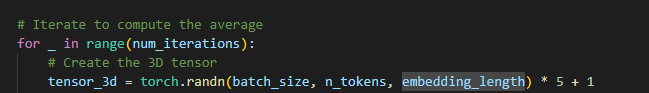
\includegraphics[width=0.8\textwidth]{./normalization_demo_tensor.png} % Adjust the width as needed
\end{figure}
Where batch size = 5, n tokens = 3, embedding length = 4. The following are its sample means and variances:
\begin{figure}[H]
    \centering
    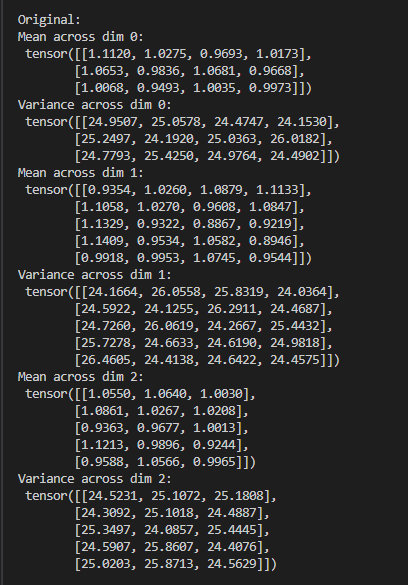
\includegraphics[width=0.8\textwidth]{./original_tensor.png} % Adjust the width as needed
\end{figure}
If we do batch normalization, the means and variances change to this: 

\begin{figure}[H]
    \centering
    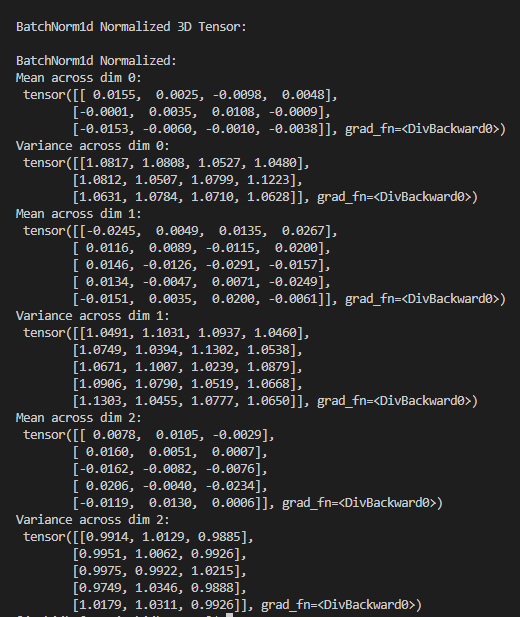
\includegraphics[width=0.8\textwidth]{./batchnormed.png} % Adjust the width as needed
\end{figure}

Note that in this case the means and variances of dimensions 1 and 2 also change, but that is because we generated this array from uncorrelated gaussian noise and therefore there's 0 covariance between any of the features (dimension 2) and also 0 covariance between the different tokens (dimension 1). this wouldn't be the case if we were dealing with tokenized natural language inputs already passed through an embedding layer. In that case, we'd see batchnorm normalizing across dimension 0 but not across 1 and 2, and layer normalization normalizing across dimension 2 but not across dimension 1 or 0. 


\subsubsection{Why Batchnorm Solves Exploding Gradients} 
The equation for batchnorm is:

\[ \hat{x}_i = \frac{x_i - \mu_B}{\sqrt{\sigma_B^2 + \epsilon}} \]
And typically the output \(\hat{x}\) is scaled and shifted with learnable parameters \(\gamma\) and \(\beta\):

\[y = \gamma \hat{x} + \beta\]

When we do backpropagation via the chain rule, it typically looks something like this: 

\[\frac{\partial \mathcal{L}}{\partial x} = \frac{\partial \mathcal{L}}{\partial y} \cdot \frac{\partial y}{\partial \hat{x}} \cdot \frac{\partial \hat{x}}{\partial x}\]

\[\frac{\partial y}{\partial \hat{x}}  = \gamma\]

And then:

\[\frac{\partial \hat{x}}{\partial x} = \frac{1}{\sqrt{\sigma_B^2 + \epsilon}}\left(1 - \frac{\hat{x}}{m} \right)\]

where m is the batch size. This will help stabilitze the gradient by continually scaling it by the variance of the batch. This will keep the variance in check and prevent gradients from exploding. 

\section{Layer Normalization}
Layer normalization is a technique in which each individual vector embedding within each individual sample gets normalized.  So if we have a tensor of shape:

\[\mathbb{T}\text{.shape} = (12, 1024, 768)\]

Where batch size is 12, block size (N tokens) is 1024, and the embedding dimension (N embd) is 768, then layer normalization would take each \((1024, 768)\) matrix and normalize each 768-length row of that matrix to have a mean of 0 and a variance of 1.

\begin{figure}[H]
    \centering
    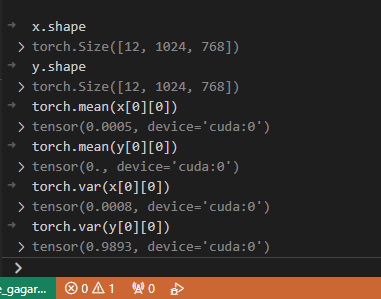
\includegraphics[width=0.8\textwidth]{./layer_norm_ex.png} % Adjust the Poidth as needed
    \caption{An example of layer normalization. Variable X is before LayerNorm, Y is after.}
\end{figure}



\textbf{Why is Layer Normalization used in Transformers?} \\
Layer Normalization is useful in transformers because we're normalizing across each token's individual vector embedding, to make sure that it has a mean of 0 and a variance of 1. If we were using batch normalization we'd be normalizing across all sequences in a batch, which is less useful. Batchnorm is more useful for CNNs because the variation between samples is likely to be a major source of unecessary noise. In language models, we can't really do batchnorm because sequences may be of different lengths, but also variation between token embeddings is more important to control.

\section{Natural Language Processing}
\subsection{Basic Paradigms}
There are three basic NLP paradigms: 
\begin{enumerate}
	\item \textbf{Vector to Sequence}: Input a vector of data, generate a natural language sequence of outputs (e.g: image captioning)
	\item \textbf{Sequence to Vector}: Given a natural language sequence as input, generate a vector as output (e.g: sentiment analysis)
	\item \textbf{Sequence to Sequence}: Given a natural language sequence as input, generate another sequence as output (e.g: translation, chatbots)
\end{enumerate}
RNNs, LSTMs, and Transformers can be used for all three of these. But their exact implementations will differ depending on which paradigm we're applying them to.

\section{Frechet Inception Distance}
Frechet Inception Distance (FID) is a metric used to evaluate the quality of images generated by models, particularly in generative adversarial networks (GANs). It measures the similarity between the distribution of generated images and the distribution of real images, utilizing the feature space of a specific layer in the Inception network. Frechet Inception Distance is based on Frechet Distance. The Frechet Distance between two Gaussians is given by:

\[FID = ||\mu_r - \mu_g ||^2 + \text{Tr}(\Sigma_r + \Sigma_g - 2(\Sigma_r\Sigma_g)^{\frac{1}{2}})\]



Where \(\mu_r, \Sigma_r\) Are the mean and variance of the real image, and \(\mu_g, \Sigma_g\), are the mean and covariance matrices of the generated image. Tr() denotes the trace operation. \textbf{Note}: the mean and covariance are calculated across the entire set of real and generated images, not for individual images. Also, it's worth noting that rather than computing a direct pixel-by-pixel mean, in practice, FID score is usually calculated on higher level feature vectors extracted via a prectrained Inception Network, which gives more meaningful distance metrics than we would get from raw pixels.

\subsection{Why this works}

Note the striking similarities between this equation and the loss function for Neural Style Transfer (Gatys et al.). There are deep connections in how information can be extracted from feature spaces in computer vision. Specifically, the first term \(||\mu_r - \mu_g ||^2\) captures global, large scale content differences between the real and generated images, while the 2nd term \(\text{Tr}(\Sigma_r + \Sigma_g - 2(\Sigma_r\Sigma_g)^{\frac{1}{2}})\) is almost exactly equivalent to the style component in neural style transfer. The more similarly the two matrices covariances are, then the more stylistic patterns are shared in common between the two images.\\

In other words, we have exactly the same principles at play in both Neural Style Transfer and FID (the capturing of both content and style differences between two images). in the former this is used as a loss function to drive a gradient descent process that results in style transfer between two domains; in the latter, this is used to quantify the extent to which a generated image diverges from how it should 'really' look. 

\section{Recurrent Neural Nets}

Traditional neural nets are very bad at making predictions on sequential or time series data. Why? Because traditional neural nets don't retain past or historical information, they treat each observation as independent. Recurrent Neural Nets attempt to solve this problem. Transformers really solve it (see above). But RNNs are important to understand too.

RNNs have both spatial and temporal dimensions. The spatial dimension is exactly the same as a normal neural net. It may be deep (multiple layers stacked atop each other) or shallow (just a single layer). It has an input \(x_t\) and an output \(\hat{y}_t\). The temporal dimension is what makes RNNs special. Mathematically, it is a recurrance relation (a function in which the output at the \(t^{th}\) timestep is a function of the outputs of the preceeding timesteps:

\[a_t = \varphi(t, a_{n-k}) \text{ for } t > 0, k = 1, \varphi: \mathbb{T}\times X \rightarrow X\]

Where k typically equals 1 (some fancier versions of RNNs utilize skip connections or other things to improve stability) and \(X\) is the set to which the elements \(a_{n-k}\) must belong. \\

Intuitively, RNNs can be thought of as a 'temporally deep' network. In the example of sentiment analysis, we feed the words through them sequentially, and each 'layer' (each timestep), the RNN cell accepts the output from the previous timestep as an input as well as the token at the current timestep. Each word is represented as a timestep. The temporal dimension is what enables RNNs to express complicated sequential relationships between timesteps despite the fact that they may only have one layer (they can be thought of as representing a 'temporally deep' network). However, it also makes them unstable, as we'll discuss shortly.

\begin{figure}[H]
    \centering
    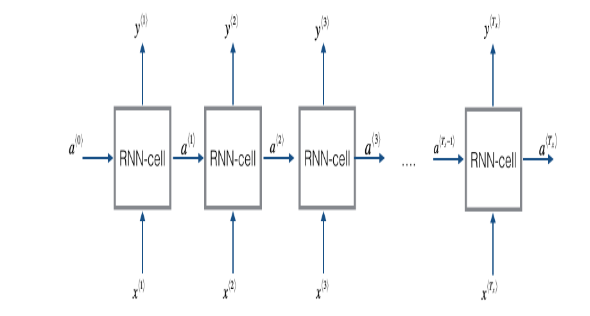
\includegraphics[width=0.8\textwidth]{./RNN_network.png} % Adjust the Poidth as needed
    \caption{Several timesteps of an RNN unfolded. Note that this is THE SAME network and that the timesteps are processed IN SERIAL. One cell (or one network if it is deep) symbolically represents each of the boxes. If this network were deep, the layers would be stacked vertically atop the cell at each timestep (note again that there is only one cell. it gets new information fed into it at each timestep.}
\end{figure}



\subsection{How it works}

This is the formula for a single-layer RNN cell:

\begin{figure}[H]
    \centering
    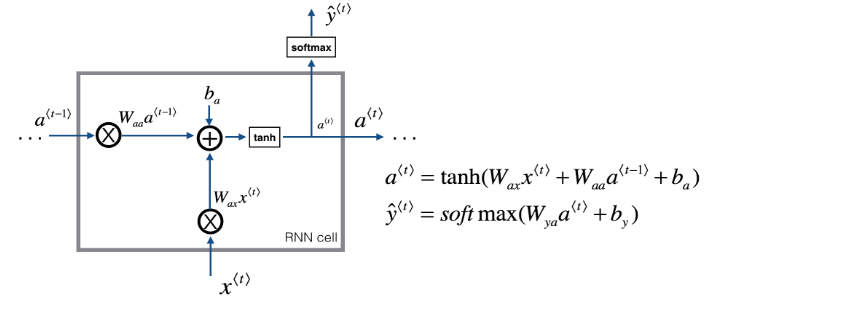
\includegraphics[width=0.8\textwidth]{./RNN_cell.png} % Adjust the Poidth as needed
\end{figure}

\(a^{\langle t-1\rangle}\) represents the activation function of that same cell at the previous timestep. \(x^{\langle t\rangle}\) is the input to the network at the current timestep. If we were processing the sentence "My name is Jared", and \(t=3\), then \(a^{\langle t-1\rangle} = \) RNN(is) and \(x^{\langle t\rangle} = \) Jared. \(W_{aa}\) is the weights matrix for the temporal input. \(W_{ax}\) are the weights for the normal input. \\

If we had multiple layers in our network, \(x_{l=0}^{\langle t\rangle} = \) Jared and then the next layer \(x_{l=1}^{\langle t\rangle} = a^{\langle t\rangle}\):

\[a_i^{\langle t \rangle} = tanh(W_{ax}^{[i]}x_{i-1}^{\langle t \rangle} + W_{aa}^{[i]}a_i^{\langle t-1 \rangle} + b_a^{[i]})\]

 Note that we only have softmax after the final vertical layer in the event of a Deep RNN. This means layer \(L_{i+1}^{\langle t \rangle}\) receives \(a_i^{\langle t \rangle}\) as its depthwise input \(x^{\langle t\rangle}\) and \(L_{i}^{\langle t+1 \rangle}\) also receives the same thing as its temporal input \(a^{\langle t- 1\rangle}\).\\

\textbf{Computations in a single-layer RNN temporal Step}:
\begin{enumerate}
\item Compute the hidden state with tanh activation \(a^{\langle t\rangle} = tanh(W_{aa}a^{\langle t-1\rangle} + W_{ax}x^{\langle t\rangle} + b_a)\)
\item Using your new hidden state \(a^{\langle t\rangle}\), compute the prediction \(\hat{y^{\langle t \rangle}} = softmax(W_{ya}a^{\langle t\rangle} + b_y)\)
\item store (\(a^{\langle t\rangle}, a^{\langle t-1\rangle}, x^{\langle t\rangle}, W_{aa}, W_{ax}, W_{ya}, b_a, b_y\)) in cache for backpropagation.
\item return \(a^{\langle t\rangle}\), \(\hat{y}^{\langle t \rangle}\), and cache
\end{enumerate}

\begin{figure}[H]
    \centering
    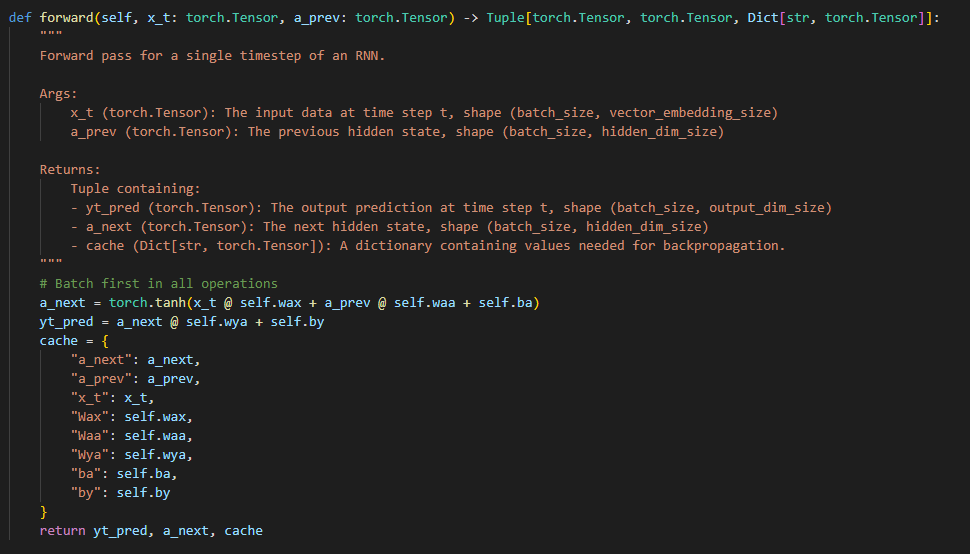
\includegraphics[width=1.0\textwidth]{./RNN_forward_pass_python.png} % Adjust the Poidth as needed
	\caption{A forward pass through a single timestep of a RNN}
\end{figure}

\begin{figure}[H]
    \centering
    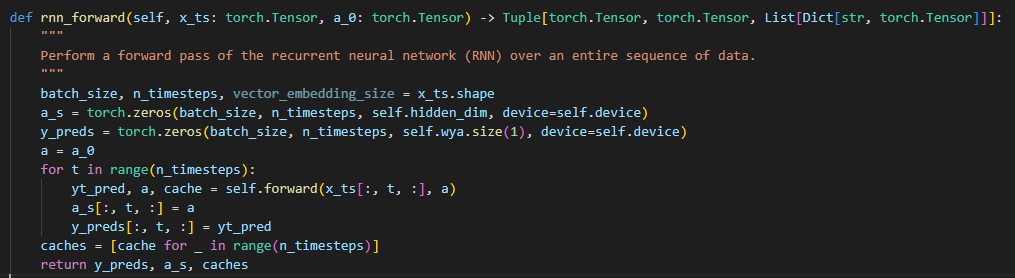
\includegraphics[width=1.0\textwidth]{./RNN_net_full_pass.png} % Adjust the Poidth as needed
	\caption{A forward pass through the full RNN}
\end{figure}



\subsection{Backpropagation Through Time}

In backgpropagation through time, we compute the total accumulated loss across all \(\tau\) timesteps and then update the weights once (only once! It may sound like we need to update the weights \(\tau\) times given that we have \(\tau\) timesteps, but no). Accordingly, the gradients for each of our learnable parameters can be expressed as a combination of sums and products:

\[
\frac{\partial \mathcal{J}}{\partial W_{ax}} = \sum_{k=1}^{\tau} \frac{\partial \mathcal{J}}{\partial a^{\langle \tau \rangle}} \left( \frac{\partial a^{\langle \tau \rangle}}{\partial a^{\langle k \rangle}} \right) \frac{\partial a^{\langle k \rangle}}{\partial W_{ax}}
\]

\[\frac{\partial J}{\partial W_{aa}} = \sum_{k=1}^\tau \frac{\partial J}{\partial a^{\langle \tau \rangle}} \left( \frac{\partial a^{\langle \tau \rangle}}{\partial a^{\langle k \rangle}} \right) \frac{\partial a^{\langle k \rangle}}{\partial W_{aa}}\]


\[\frac{\partial \mathcal{J}}{\partial b_{a}} = \sum_{k=1}^{\tau} \frac{\partial \mathcal{J}}{\partial a^{\langle \tau \rangle}} \left( \frac{\partial a^{\langle \tau \rangle}}{\partial a^{\langle k \rangle}} \right) \frac{\partial a^{\langle k \rangle}}{\partial b_{a}}
\]

Where 

\[\frac{\partial a^{\langle \tau \rangle}}{\partial a^{\langle k \rangle}} = \prod_{i=k+1}^{\tau} \frac{\partial a ^{\langle i \rangle}}{\partial a ^{\langle i - 1 \rangle}} = \prod_{i=k+1}^{\tau}W_{aa} \cdot (1-\tanh(W_{ax}x^{\langle i \rangle} +W_{aa}a^{\langle i-1\rangle}+b_a)^2) \]

Note that \(\frac{\partial \mathcal{J}}{\partial a^{\langle \tau \rangle}}\) is the gradient of the loss \(J\) with respect to the temporal output of our final timestep \(a^{(\tau)}\), \(\frac{\partial a^{\langle \tau \rangle}}{\partial a^{\langle k \rangle}}\) is the gradient of the temporal output of our final timestep with respect to the temporal output of our current timestep; and then the final term in each summation is the gradient of the temporal output of our current timestep with respect to the learnable parameters we wish to update. Each of these is: 

\[\frac{\partial a^{\langle k \rangle}}{\partial W_{ax}} = (1 - \tanh(W_{ax}x^{\langle k \rangle} + W_{aa}a^{\langle k-1\rangle} + b_a)^2) x^{\langle k \rangle T}\] 

\[\frac{\partial a^{\langle k \rangle}}{\partial W_{aa}}  = (1-tanh(W_{ax}x^{\langle k \rangle} +W_{aa}a^{\langle k-1\rangle}+b_a)^2)a^{\langle k- 1\rangle T}\]
\[\frac{\partial a^{\langle k \rangle}}{\partial b_{a}} = (1-tanh(W_{ax}x^{\langle k \rangle} +W_{aa}a^{\langle k-1\rangle}+b_a)^2)\]

Let's assume we're doing sentiment analysis (classification) and our loss function is categorical crossentropy with a softmax output following the final timestep. This means that the gradient of the loss with respect to the output of our \(\tau^{th}\) layer is:

\[\frac{\partial J}{\partial a^{\langle \tau \rangle}} = \hat{y}_c^{\langle t \rangle} - y_c^{\langle t \rangle} \]

Where \(c\) denotes the element-wise subtraction across each class \(c\) in our classification problem. Now, let's combine all of these terms together for just one of the parameters above so we can see what the full update equation for BPTT actually looks like: 

\[\frac{\partial \mathcal{J}}{\partial W_{ax}} = \sum_{k=1}^{\tau} \left( \hat{y}_c^{\langle \tau \rangle} - y_c^{\langle \tau \rangle}  \right) \left( \prod_{i=k+1}^{\tau}W_{aa} \cdot (1-\tanh(W_{ax}x^{\langle i \rangle} +W_{aa}a^{\langle i-1\rangle}+b_a)^2) \right) \frac{\partial a^{\langle k \rangle}}{\partial W_{ax}}\]

Where, as before: 
\[\frac{\partial a^{\langle k \rangle}}{\partial W_{ax}} = (1 - \tanh(W_{ax}x^{\langle k \rangle} + W_{aa}a^{\langle k-1\rangle} + b_a)^2) x^{\langle k \rangle T}\] 

This update gets applied ONCE across all timesteps. And that's how backpropagation through time works!

\subsection{Why RNNs tend to be unstable}

Notice that all our gradients above depend on 

\[\frac{\partial a^{\langle \tau \rangle}}{\partial a^{\langle k \rangle}} = \prod_{i=k+1}^{\tau} \frac{\partial a ^{\langle i \rangle}}{\partial a ^{\langle i - 1 \rangle}}\]


Substituting in the direct algebraic expression this gradient, we have

\begin{align*}
\frac{\partial a^{\langle \tau \rangle}}{\partial a^{\langle k \rangle}} &= \prod_{i=k+1}^{\tau}W_{aa} \cdot (1-\tanh(W_{ax}x^{\langle i \rangle} +W_{aa}a^{\langle i-1\rangle}+b_a)^2) \\
&= W_{aa}^{(\tau - k + 1)}\prod_{i=k+1}^{\tau}(1-\tanh(W_{ax}x^{\langle i \rangle} +W_{aa}a^{\langle i-1\rangle}+b_a)^2)
\end{align*}

As \(\tau - k + 1 \rightarrow \infty\), 
\[W_{aa}^{(\tau - k + 1)} = \begin{cases} \infty: & W > 1 \\ 0: & W<1 \end{cases}\]

And we have a vanishing/exploding gradient.\\

Why is this not a problem with all kinds of deep neural nets, why specifically is this a problem with RNNs? Because the weights \(W\) in an RNN are the same in all 'layers' of the network, which is different than in a CNN or MLP. This means RNNs frequently have problems with Vanishing/Exploding Gradients.\textbf{ This problem is what LSTMs were created to solve}.

\section{LSTMs}
LSTMS solve the vanishing/exploring gradient problem that plagues RNNs. They do this by controlling the flow of information between timesteps. LSTMs can have multiple spatial layers or just one, same as an RNN. Unlike an RNN, a single layer can consist of multiple cells that operate in parallel of each other. each one of these single-cell, multiple layer entities is a full independent recurrent neural network with a sophisticated gated function (as mentioned) regulating the flow of information across the temporal dimension. Let's start by just focusing on a single cell, single layer LSTM:

\subsection{The LSTM Cell}

\begin{figure}[H]
    \centering
    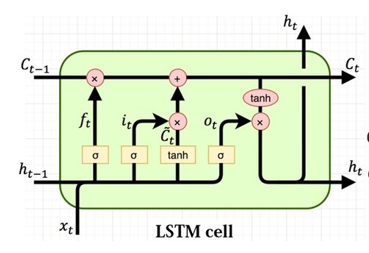
\includegraphics[width=0.8\textwidth]{./lstm_cell.png} % Adjust the Poidth as needed\end{figure}
\end{figure}
The key components of the LSTM cell at time step \(t\) include:

\textbf{Forget Gate} (\(f_t\)): Determines which parts of the cell state \(C_{t-1}\) should be forgotten.
\begin{equation}
    f_t = \sigma(W_f \cdot [h_{t-1}, x_t] + b_f)
\end{equation}

\textbf{Input Gate} (\(i_t\)): Decides which new information will be stored in the cell state.
\begin{equation}
    i_t = \sigma(W_i \cdot [h_{t-1}, x_t] + b_i)
\end{equation}

\textbf{Cell State Candidates} (\(\tilde{C}_t\)): Creates a vector of new candidate values that could be added to the cell state.
\begin{equation}
    \tilde{C}_t = \tanh(W_C \cdot [h_{t-1}, x_t] + b_C)
\end{equation}

\textbf{Cell State Update} (\(C_t\)): Updates the old cell state \(C_{t-1}\) into the new cell state \(C_t\).
\begin{equation}
    C_t = f_t \ast C_{t-1} + i_t \ast \tilde{C}_t
\end{equation}

\textbf{Output Gate} (\(o_t\)): Decides what part of the cell state will be outputted.
\begin{equation}
    o_t = \sigma(W_o \cdot [h_{t-1}, x_t] + b_o)
\end{equation}

\textbf{Hidden State} (\(h_t\)): The hidden state and output of the LSTM cell at time step \(t\).
\begin{equation}
    h_t = o_t \ast \tanh(C_t)
\end{equation}
 Each LSTM cell contains 3 gates: 
\begin{enumerate}
	\item \begin{figure}[H] \centering 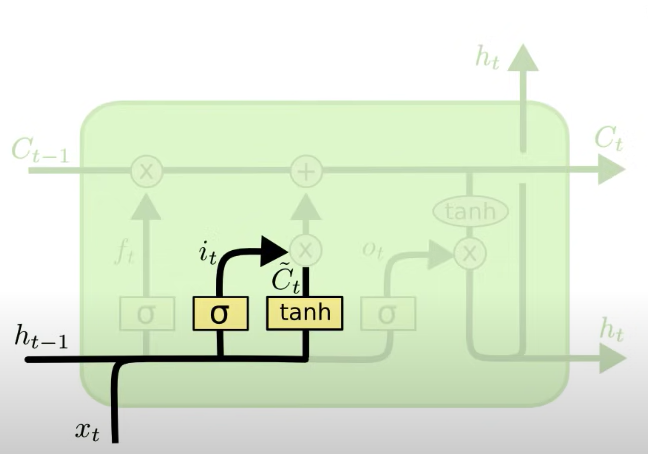
\includegraphics[width=0.7\textwidth]{./lstm_input_gate.png} \caption{\textbf{Input Gate}: Controls whether cell state is updated. Imagine if \(i_t\) were 0. Then obviously nothing new would be added to cell state} \end{figure}
	\item  \begin{figure}[H] \centering 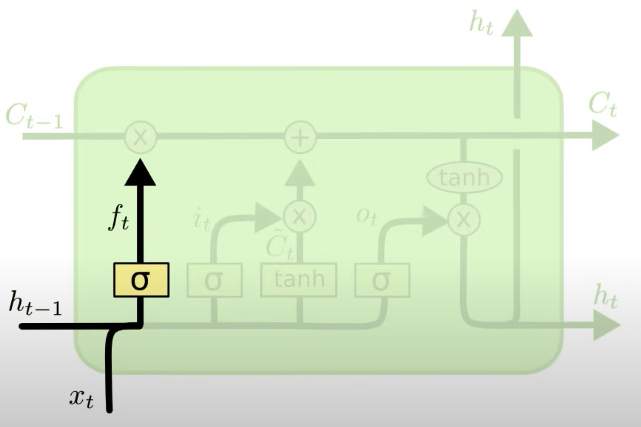
\includegraphics[width=0.7\textwidth]{./lstm_forget_gate.png} \caption{\textbf{Forget Gate}: Controls whether (and to what extent) elements of cell state are forgotten. Imagine if \(f_t\) were 0. Then obviously the old cell state \(C_{t-1}\) would be completely forgotten.} \end{figure}
	\item \begin{figure}[H] \centering 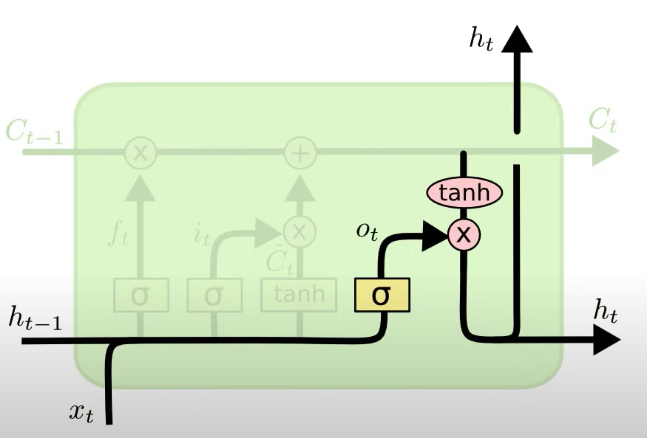
\includegraphics[width=0.7\textwidth]{./lstm_output_gate.png} \caption{\textbf{Output Gate}: Controls whether hidden state \(h_t\) is exported to next timestep. Imagine if \(o_t\) were 0. Then obviously the output hidden state \(h_t\) would be 0. Notice the output gate reads from \(C_t\) but does not write to it.} \end{figure}
\end{enumerate}
\(C_t\) Can be thought of as the long term memory. \(h_t\) can be thought of as the short term memory (it gets recalculated each timestep and while it may influence the computation of hidden values many layers in advance it cannot directly be propagated forward unmodified past timestep \(t+1\). \\

Each of the functions defining the gates is differentiable (because of the sigmoid function) and thus gradients flow through them. If gradients flow through them, then the weights will be updated in such a way that the loss will decrease as a result of the weight updates being applied. It doesn’t seem possible that this network could learn to use the gates. But it can.

\subsection{Why LSTMs work}

Consider the two pieces of information that get passed forward from timestep to timestep: cell state \(C_t\) and hidden state \(h_t\). As shown above, this is the equation for updating \(C_t\):

\[C_t = f_t \odot C_{t-1} + i_t \odot \tilde{C}_t\]

Where \(f_t\) is the computed value of the forget gate, \(i_t\) is the computed value of the input gate, and \(\tilde{C}_t\) is the computed value of the cell state candidates. The gradient of current cell state with respect to the previous is:
\[\frac{\partial C_t}{\partial C_{t-1}} = f_t\]

Because the 2nd term (\(i_t \odot \tilde{C}_t\)) does not directly depend on \(C_{t-1}\). This means that if we extent this propagation through \(\tau\) timesteps we get: 

\[\frac{\partial C_\tau}{\partial C_{t}} = \prod_{k=t}^\tau f_k\]

\(f_t\) can differ in each timestep \(t\) because \(f_t\) is a function of the input at timestep \(t\) \(x_t\). This means that the gradient won't explode even as \(\tau\) gets very large. Since \(f_t\) is the output of a sigmoid function, it is bounded between 0 and 1 and it can learn to set \(f_t\) values close to 1, allowing the gradient to pass through almost unchanged if information is relevant, meaning it will enither vanish nor explode. \\

Long Short-Term Memory (LSTM) networks are specifically designed to address the vanishing and exploding gradient problems that are common in vanilla Recurrent Neural Networks (RNNs). The core of this design lies in the LSTM's gating mechanisms, which regulate the flow of information. We will explore the mathematical foundation that provides LSTMs with their gradient stability.

The hidden state \( h_t \) in an LSTM is computed as:

\begin{equation}
h_t = o_t \odot \tanh(C_t)
\end{equation}

where \( o_t \) is the output gate's activation, and \( C_t \) is the cell state at time \( t \).

The gradient of \( h_t \) with respect to the previous hidden state \( h_{t-1} \) involves derivatives that are functions of both \( o_t \) and \( C_t \):

\begin{equation}
\frac{\partial h_t}{\partial h_{t-1}} = \frac{\partial h_t}{\partial o_t} \frac{\partial o_t}{\partial h_{t-1}} + \frac{\partial h_t}{\partial C_t} \frac{\partial C_t}{\partial h_{t-1}}
\end{equation}

This can be further decomposed into:

\begin{equation}
\frac{\partial h_t}{\partial o_t} = \tanh(C_t)
\end{equation}

\begin{equation}
\frac{\partial o_t}{\partial h_{t-1}} = o_t \odot (1 - o_t) \text{ (scaled by the relevant weights)}
\end{equation}

\begin{equation}
\frac{\partial h_t}{\partial C_t} = 1 - \tanh^2(C_t)
\end{equation}

The complexity of \( \frac{\partial C_t}{\partial h_{t-1}} \) is mitigated by the LSTM's structure, where each gate's activation function bounds the gradients.

When backpropagating over multiple timesteps, we compute:

\begin{equation}
\frac{\partial h_t}{\partial h_{t-n}} = \prod_{k=t-n+1}^{t} \left( \frac{\partial h_k}{\partial h_{k-1}} \right)
\end{equation}

The LSTM gates—\( f_t \), \( i_t \), and \( o_t \)—use sigmoid and tanh functions that inherently bound the values and gradients, thus stabilizing the backpropagated gradients:

\begin{itemize}
\item The \textit{forget gate} \( f_t \) allows the network to retain or forget information selectively, preventing gradients from diminishing too rapidly.
\item The \textit{output gate} \( o_t \) controls the impact of the cell state on the hidden state and the propagated gradients, preventing them from growing excessively.
\item The \textit{input gate} \( i_t \) integrates new input into the cell state, allowing the network to adapt to new information without being destabilized by past gradients.
\end{itemize}

Furthermore, because the gates are controlled by learnable parameters with gradients flowering through them, the network WILL learn to use them in such a way that minimizes loss (i.e inherently involves preventing vanishing/exploding gradients). Don't believe me? I didn't at first either, but a cool, very meta way of thinking about this helped me out: "Sure, it COULD learn this behavior. Why would it?" The answer is that the best way to operate the gates is going to be the one that minimizes the loss function. The behavior that minimizes the loss function will prevent vanishing/exploding gradients from messing up the performance of the network. Retaining useful information, discarding useless information, and making sure the gradients stay within reasonable bounds (i.e near 1) for info that needs to be propagated forward. Therefore, if you believe it is possible to use these gates to prevent vanishing/exploding gradients and believe that doing so would result in a network with better performance (lower loss) then you know how the gates will operate in such a way that minimizes loss.\\

Each of these functions is differentiable and thus gradients flow through them. If gradients flow through them, then the weights will be updated in such a way that the loss will decrease as a result of the weight updates being applied. It doesn’t seem possible that this network could learn to use the gates. But it can.

\section{Skewness}

Skewness is a measure of the asymmetry of the probability distribution of a real-valued random variable about its mean, offering insights into the distribution's shape.

\subsection{Mathematical Definition}

The skewness (\(S\)) of a random variable's probability distribution is defined as:

\[ S = \frac{E[(X - \mu)^3]}{\sigma^3} \]

where \(E[(X - \mu)^3]\) is the third statistical moment of the distribution, \(\mu\) is the mean, and \(\sigma\) is the standard deviation. Recall that: 
\[E[(X - \mu)^3] = \int (x - \mu)^3 f(x) dx\]
For continuous PDFs and 
\[E[(X - \mu)^3] = \sum_{i=1}^{n} (x_i - \mu)^3\]
For discrete PDFs

This means that if you really want to see all the math we can expand our definition of skewness to:

\[ S = \frac{\int (x - \mu)^3 f(x) dx}{(\int (x - \mu)^2 f(x) dx)^{\frac{3}{2}}} \]

And for a discrete distribution:

\[ S = \frac{\frac{1}{n}\sum_{i=1}^{n} (x_i - \mu)^3}{\left(\frac{1}{n}\sum_{i=1}^{n} (x_i - \mu)^2\right)^{\frac{3}{2}}} \]



Because the second statistical moment  \(E[(X - \mu)^2] = Var(X) = \sigma_X^2\). (Note: we multiply both Expectations by \(\frac{1}{n}\) because that's how we calculate the expectation for discrete pdfs. Also note that \(\frac{1}{n} \div \left(\frac{1}{n}\right)^{\frac{3}{2}} = \frac{1}{\sqrt{n}} \neq 1\).

\subsection{Explanation of What It Measures}

Skewness quantifies the degree of asymmetry of a distribution around its mean:
\begin{itemize}
    \item A \textbf{positive skewness} indicates a distribution with a tail that extends towards more positive values.
    \item A \textbf{negative skewness} shows a distribution with a tail that extends towards more negative values.
    \item A \textbf{skewness of 0} implies a perfectly symmetric distribution.
\end{itemize}

\subsection{When to Use It}

Skewness is utilized in data analysis to assess the distribution shape, in model assumptions to check for normality, and in outlier detection, providing a foundational understanding for statistical modeling and analysis.
\section{Hooks}
Hooks are functions that can be injected into a neural network an automatically perform logging, visualization, or other operations in the forward or back pass. They are directly attached to specific layer(s) of a neural network, and execute during that layer's foreward or back pass.\\

They are extremely useful as a debugging tool. Hooks can also be injected into trainer objects to enhance the modularity and extensibility of train loops. Here is sample code for defining a simple hook function and injecting it into the linear layers of a MLP: 

\begin{figure}[H] \centering \includegraphics[width=0.9\textwidth]{./add\_hook\_fn.png} \caption{After calling this method with a function handle, this will add the hook directly to the specified module of the MLP} 
\end{figure}

\begin{figure}[H] \centering \includegraphics[width=0.9\textwidth]{./call\_hook\_fn.png} \caption{The register\_hook method for torch.nn.Module is built-in, so this hook will automatically be called by pytorch.} 
\end{figure}

And here is code showing how to call this add\_hook method: 


\section{Kurtosis}

Kurtosis is a statistical measure that describes the shape of a probability distribution's tails in relation to its peak, often interpreted as a measure of the distribution's "tailedness."

\subsection{Mathematical Definition}

Kurtosis is defined as the normalized fourth central moment of a distribution:

\[ \text{Kurtosis} = \frac{E[(X - \mu)^4]}{\sigma^4} \]

where \(E[(X - \mu)^4]\) is the fourth central moment, \(\mu\) is the mean of the distribution, and \(\sigma\) is the standard deviation. This definition means that kurtosis is a dimensionless quantity, normalized by the square of the variance (\(\sigma^4\)), making it independent of the scale of the distribution.

\subsection{What It Measures}

Kurtosis captures the weight of a distribution's tails in comparison to its peak:
\begin{itemize}
    \item \textbf{High Kurtosis} (\(> 3\)) indicates a distribution with heavy tails and a sharp peak, suggesting the presence of outliers.
    \item \textbf{Low Kurtosis} (\(< 3\)) signifies a distribution with light tails and a more flat peak, implying fewer outliers.
    \item \textbf{Normal Kurtosis} (\(= 3\)) for a normal distribution. This value serves as a reference point, with excess kurtosis often calculated as \(\text{Kurtosis} - 3\) to measure deviation from normality.
\end{itemize}

\subsection{When to Use It}

Kurtosis is particularly useful in:
\begin{itemize}
    \item Identifying the presence of outliers, with higher kurtosis indicating a higher likelihood of outliers in the data.
    \item Assessing the risk in financial models, as distributions with higher kurtosis are associated with more extreme events.
    \item Comparing the tails of different distributions, to understand their propensity towards producing values far from the mean.
\end{itemize}
\section{Boosting}

Boosting is an ensemble meta-algorithm in machine learning that transforms a collection of weak learners into a strong learner, iteratively focusing on the errors of previous models to improve overall accuracy.

\subsection{Step-by-Step Process}

\begin{enumerate}
    \item \textbf{Initialization}: Begin with a dataset and assign equal weights to all data points.
    \item \textbf{Train the First Learner}: A weak learner, such as a decision stump, is trained on the data.
    \item \textbf{Evaluate and Update Weights}: The performance of the model is evaluated, and the weights of the misclassified data points are increased.
    \item \textbf{Train Subsequent Learners}: New models are trained on the reweighted data, each time focusing more on the previously misclassified instances.
    \item \textbf{Combine Learners}: The individual models are combined into a single model, where each one's vote is weighted by its accuracy.
    \item \textbf{Iterate}: Repeat steps 3–5 until the performance improvement is satisfactory or a predetermined number of models have been trained.
\end{enumerate}

\subsection{Mathematical Weighting of Misclassified Examples}

In boosting, the weighting of misclassified examples is adjusted mathematically by increasing their weights in the distribution on which subsequent learners are trained.In many boosting algorithms, such as AdaBoost, each training example contributes to the overall loss that the algorithm is trying to minimize. The weight of each example determines how much its contribution to the loss is. If a data point is misclassified, its weight is increased, thereby increasing its contribution to the total loss. If \(D_i\) is the distribution used to train the \(i\)-th model, and \(w_j\) is the weight of the \(j\)-th data point, then after training, the weights are updated using the rule:

\[ w_j := w_j \cdot \exp(\alpha_i \cdot I(y_j \neq h_i(x_j))) \]

where \(I\) is an indicator function that is 1 if the \(j\)-th data point is misclassified by the \(i\)-th model and 0 otherwise, \(h_i(x_j)\) is the prediction of the \(i\)-th model for the \(j\)-th data point, \(y_j\) is the true label, and \(\alpha_i\) is the performance weight of the \(i\)-th model.

\subsection{Weighting Models by Performance}

The final prediction of the boosted ensemble is typically a weighted sum of the predictions of the individual models, where the weights are determined by the models' accuracy. The weight \(\alpha_i\) for the \(i\)-th model can be calculated as:

\[ \alpha_i = \frac{1}{2} \log \left(\frac{1 - \text{error}_i}{\text{error}_i}\right) \]

where \(\text{error}_i\) is the weighted error rate of the \(i\)-th model on the training set. The logarithmic function ensures that models with lower error rates have higher weights.
\subsection{Pseudocode for Adaboost}

\begin{enumerate}
    \item \textbf{Input}: Training data $\{(x_i, y_i)\}_{i=1}^N$ where $x_i \in \mathbb{R}^d$ and $y_i \in \{-1, +1\}$
    \item \textbf{Initialize}:
    \begin{itemize}
        \item Initialize weights $w_i = \frac{1}{N}$ for all $i = 1, \ldots, N$
    \end{itemize}
    \item \textbf{For} $t = 1$ to $T$ \textbf{do}:
    \begin{enumerate}
        \item Train a weak learner $h_t(x)$ using the weighted training data
        \item Compute the weighted error of the weak learner:
        \[
        \epsilon_t = \frac{\sum_{i=1}^N w_i \cdot \mathbf{1}(y_i \neq h_t(x_i))}{\sum_{i=1}^N w_i}
        \]
        where $\mathbf{1}(\cdot)$ is the indicator function
        \item Compute the weight of the weak learner:
        \[
        \alpha_t = \frac{1}{2} \ln \left( \frac{1 - \epsilon_t}{\epsilon_t} \right)
        \]
        \item Update the weights for the training data:
        \[
        w_i \leftarrow w_i \cdot \exp(-\alpha_t y_i h_t(x_i)) \quad \text{for all } i = 1, \ldots, N
        \]
        \item Normalize the weights:
        \[
        w_i \leftarrow \frac{w_i}{\sum_{j=1}^N w_j}
        \]
    \end{enumerate}
    \item \textbf{End For}
    \item \textbf{Output}:
    \begin{itemize}
        \item The final strong classifier:
        \[
        H(x) = \text{sign} \left( \sum_{t=1}^T \alpha_t h_t(x) \right)
        \]
    \end{itemize}
\end{enumerate}

\subsection{When to Use and Not to Use Boosting}

\textbf{When to Use}:
\begin{itemize}
    \item When dealing with bias problems where a complex model is needed.
    \item In classification problems with imbalanced classes.
    \item When the dataset is relatively free of noise.
\end{itemize}

\textbf{When Not to Use}:
\begin{itemize}
    \item With noisy datasets, as it may lead to overemphasis on noise.
    \item Where computational efficiency is a primary concern.
    \item When a simpler model would be adequate.
\end{itemize}
\section {Dataset Contamination \& Detecting via Distance Distribution}
Dataset contamination occurs when test data leaks into the train dataset. There are two kinds of contamination:

\begin{enumerate}
\item \textbf{Explicit Contamination}: When some samples in the test data are literally just present in the training data
\item \textbf{Implicit Contamination}: When the model is trained on synthetic data generated from some other model which was trained on test data
\end{enumerate}
LLMs are particularly vulnerable to dataset contamination, because they are trained on such huge datasets and the documentation of such datasets is poor and often proprietary. Dataset contamination can lead to artificially high performance on test data and worse generalizability on real unseen data.\\ 

The method below (Edit Distance Distribution) offers a robust means of detecting Dataset contamination
\textbf{Edit Distance Distribution}:\\

Authors define a metric Edit Distrance Distribution, where Edit Distance equals the number of insertions, deletions, or substitution of a single character necessary to make two strings match:

\[s1 = abcabcd\quad s2 = abcaaaa\]
\[ED(s1, s2) = 3\]
The authors extend this to tokenized responses for LLMs: 

\[s1 = [1, 2, 3, 1, 2, 3, 4], \quad s2=[1,2,3,1,1,1,1]\]
\[ED(s1, s2) = 3\]

Then they say compute the Edit Distance Distribution \(\rho(d)\) by on \(n\) sequences of sampled texts as follows:

\[\rho(d) = \frac{\sum_{i=1}^{n-1}\sum_{j=i+1}^{n}\mathbb{I}(ED(s_i, s_j) = d)}{n*(n-1)/2}\]

Given n sampled sequences, P(d) gives fractoion of times two samples have edit distance = d. So it's basically just a histogram of all the Edit Distances between each pair of samples, except its been normalized to meet the requirements of a discrete PDF. \\

% figure

\textbf{But how do you actually use this to detect dataset contamination?}\\

Imagine we have some LLM \(\mathcal{M}\) and test samples from our dataset 

\[\langle x, y \rangle\]

Where \(x\) is the input to the model and \(y\) is the desired output. For each x and y, we plug x into the model, set the temperature of the model \(\tau=0\) and pass the input \(x\) through the model to get the following:

\[\mathcal{M}_{\tau=0}(x) = s_{\tau=0}\]

Then, with temperature \(\tau > 0\), we sample from the \(\mathcal{M}(s)\) \(n\) times and calculate the Edit Distance Distribution as follows:

\[\rho(d) = \frac{\sum_{i=1}^{n-1}\mathbb{I}(s_i, s_{\tau=0} = d)}{n}\]

The idea is that if the model is unduly confident of an exact response, many of its responses will have zero or low edit distance distribution even once the temperature is turned up. This distinction makes the CDD algorithm very similar to perplexity (but we don't need knonw clean and ditry benchmark datasets \(\mathcal{C}\) and \(\mathcal{D}\) to compare the perplexity of some test dataset \(\mathcal{T}\) against. Also, we calculate at the sample level rather than the dataset level, which i think allows for cleaning contaminated datasets). Once again, the idea is that the model is likely to be disproportionately confident in the output of the dataset (very low perplexity) when contamination occurs. \\

From here, the authors define the peakedness of the EDD as the proportion of samples that have an edit distance less than some cricitcal distance \(\alpha \cdot l\) using the CDF of their EDD function (which meets the definition of a PDF):

\[\text{Peak}(\mathcal{M};x) = F(d \leq \alpha \cdot l) = \sum_{d=0}^{\alpha \cdot l}\rho(d)\]

The term \(\alpha\) is a hyperparameter between 0 and 1 (they set it to \(\alpha = 0.05\) in their studies). The term \(l\) is the longest sequence length they sampled from the model. They decide whether dataset contamination has occurred by thresholding peakedness according to some parameter \(\upsilon\):

\[\text{Leaked if Peak}(\mathcal{M}, x)>\upsilon \]

This basically corresponds to deciding it is leaked if a certain proportion of the data is within some minimum distance \(d = \alpha \cdot l\).\\

Unsurprisingly, the authors perform an ablation study against other methods for evaluating dataset contamination and decide that theirs performs the best (though I believe them). It's noteworthy that perplexity actually does a better job detecting datasets with a very high degree of contamination (their method is better at detecting data with a low degree of contamination, which is harder to detect). Also, their method is the only one they surveyed that is robust to implicit contamination. 
\section{Siamese Networks}
A Siamese network is a kind of neural network that uses the same weights in tandem on two different input vectors to compute outputs, which are then compared with each other. The idea is for similar input vectors to produce similar outputs, while different input vectors produce different outputs. It is often used for things like facial recognition (matching a facial image against some pre-defined face to see if they are the same) and anomaly detection. 

\subsection{Mathematical Definition}
Given two input vectors, \(\mathbf{x}_1\) and \(\mathbf{x}_2\), a Siamese network processes these inputs through two identical subnetworks, denoted as \(f_{\theta}(\cdot)\). These subnetworks share the same parameters, \(\theta\), which ensures that they transform the inputs in the same way. Mathematically, this can be expressed as:
\[
\mathbf{h}_1 = f_{\theta}(\mathbf{x}_1), \quad \mathbf{h}_2 = f_{\theta}(\mathbf{x}_2)
\]
where \(\mathbf{h}_1\) and \(\mathbf{h}_2\) are the output vectors from the subnetworks for the inputs \(\mathbf{x}_1\) and \(\mathbf{x}_2\), respectively.

The outputs, \(\mathbf{h}_1\) and \(\mathbf{h}_2\), are then compared using a distance metric \(D(\cdot, \cdot)\), which quantifies the similarity or dissimilarity between the two input vectors. Common distance metrics include the Euclidean distance and the cosine similarity. For example, the Euclidean distance can be defined as:
\[
D(\mathbf{h}_1, \mathbf{h}_2) = \|\mathbf{h}_1 - \mathbf{h}_2\|_2 = \sqrt{\sum_{i} (\mathbf{h}_{1,i} - \mathbf{h}_{2,i})^2}
\]

The objective of training the Siamese network is to minimize a loss function that encourages similar input pairs to have a smaller distance (higher similarity) and dissimilar pairs to have a larger distance (lower similarity). This loss function is often referred to as the Contrastive Loss or Triplet Loss, depending on the specific formulation.

\subsection{Backpropagation and Learning}
Training a Siamese network involves updating the shared parameters, \(\theta\), of the subnetworks to minimize the loss function. The common approaches for defining the loss include:

1. \textbf{Contrastive Loss}: This loss function directly penalizes the network based on the distance \(D(\mathbf{h}_1, \mathbf{h}_2)\). It is typically formulated as:
\[
L(\mathbf{x}_1, \mathbf{x}_2, y) = (1 - y) \frac{1}{2} D(\mathbf{h}_1, \mathbf{h}_2)^2 + y \frac{1}{2} \max(0, m - D(\mathbf{h}_1, \mathbf{h}_2))^2
\]
where \(y\) is a binary label indicating whether the inputs are similar (\(y = 0\)) or dissimilar (\(y = 1\)), and \(m\) is a margin parameter that defines how far apart the outputs of dissimilar pairs should be.

2. \textbf{Triplet Loss}: This loss function considers three inputs: an anchor \(\mathbf{x}_a\), a positive \(\mathbf{x}_p\) (similar to the anchor), and a negative \(\mathbf{x}_n\) (dissimilar to the anchor). The loss encourages the distance between the anchor and the positive to be smaller than the distance between the anchor and the negative by at least a margin \(m\). It is defined as:
\[
L(\mathbf{x}_a, \mathbf{x}_p, \mathbf{x}_n) = \max(0, D(\mathbf{h}_a, \mathbf{h}_p) - D(\mathbf{h}_a, \mathbf{h}_n) + m)
\]
where \(\mathbf{h}_a\), \(\mathbf{h}_p\), and \(\mathbf{h}_n\) are the outputs of the network for the anchor, positive, and negative inputs, respectively.

During training, the gradients of the loss function with respect to the network parameters \(\theta\) are computed using backpropagation. Given that the subnetworks share weights, the gradients are accumulated and applied in a way that ensures the updates are consistent across both subnetworks. This is mathematically expressed as:
\[
\theta \leftarrow \theta - \eta \nabla_{\theta} L
\]
where \(\eta\) is the learning rate, and \(\nabla_{\theta} L\) represents the gradient of the loss function with respect to the shared parameters \(\theta\).


\section{Bagging (Random Forests)}

Bagging, or Bootstrap Aggregating, is an ensemble meta-algorithm in machine learning that increases the stability and accuracy of machine learning algorithms by training multiple models on random subsets of the original dataset and then averaging the predictions. When this method is applied specifically to \(n\) tree learners, it is referred to as a random forest.

\subsection{Detailed Description}

Bagging involves training a series of base learners, typically decision trees, on different randomly drawn bootstrap samples of the dataset. Let's consider a training dataset \(D\) of size \(n\). Bagging repeatedly (for \(B\) times) selects a random sample (with replacement) of the dataset and trains a new base model \(M_b\) on this sample. Each model generates predictions, and the final output prediction is typically an average (for regression) or a majority vote (for classification) of these models.

\subsection{Step-by-Step Process}

\begin{enumerate}
    \item \textbf{Bootstrap Sampling}: Generate \(B\) different bootstrap samples from the original dataset. Each sample is the same size as the original and is drawn with replacement.
    \item \textbf{Train Base Learners}: Independently train a base learner on each of these bootstrap samples.
    \item \textbf{Aggregate Predictions}: Combine the predictions from all the base learners. For a regression problem, calculate the average of the predictions. For a classification problem, use majority voting or averaging of probabilities.
    \item \textbf{Final Model}: The aggregated prediction forms the output of the bagging ensemble.
\end{enumerate}

\subsection{Why It Works}

The effectiveness of bagging comes from its ability to reduce variance without increasing bias. To see why, let's say we have \(n\) models and each model \(M_b \in (b=1,2...n)\) produces an output prediction \(Y_b(X)\) for some input. Each of these outputs \(Y_b(X)\)  is a random variable that hsa its own mean and variance. When you average the outputs of these \(n\) models, the variance of this averaged outupt is given by 

\[Var\left(\frac{1}{n}\sum_{b=1}^nY_b(X)\right)\]

If the \(n\) models are independent, the variance of the sum is the sum of the variances; however, since each model is trained on a bootstrap ssample of the same original dataset, they won't be completely indepednent. Therefore the variance of the sum is given by:

\[Var\left(\frac{1}{n}\sum_{b=1}^nY_b(X)\right) = \sum_{b=1}^nVar(Y_b(X)) + 2\sum_{i<j}Cov(Y_i(X), Y_j(X))\]

Assuming each \(Y_b\) has the same variance \(\sigma^2\) (and this is reasonable, because the expectation of the variance for each is the same given that all bootstrapped distributions are drawn from the same one, and hence have the same expectation), and also assuming that \(Cov(Y_i, Y_j) = \rho_{ij}\sigma^2 \quad \forall i \neq j\), then the formula above simplifies to:

\[Var\left(\frac{1}{n}\sum_{b=1}^nY_b(X)\right)  = \frac{1}{n^2}\left(n\sigma^2 + \sigma^2\cdot \rho \cdot n(n-1) \right)\]

Which then further simplifies to

\[Var\left(\frac{1}{n}\sum_{b=1}^nY_b(X)\right)  = \frac{1}{n}\sigma^2 + \frac{n-1}{n}\rho \sigma^2\]

This is guaranteed to be less than the variance of the output from a single model because \(\rho\) is strictly less than or equal to 1. However, if the learners are highly correlated the reduction in variance will be less significant. 

\subsection{When to Use and Not to Use Bagging}

\textbf{When to Use}:
\begin{itemize}
    \item With high variance, low bias models (e.g., deep decision trees), where the primary goal is to reduce variance.
    \item In scenarios where the model needs to be robust against the specific training set noise.
\end{itemize}

\textbf{When Not to Use}:
\begin{itemize}
    \item When the base models are biased; bagging may not effectively reduce error if the base learners are too weak.
    \item In cases where model interpretability is crucial, as the ensemble model can be more difficult to interpret than individual models.
\end{itemize}

\subsection{Differences Between Boosting and Bagging}
\begin{enumerate}
\item \textbf{bootstrapping}: In bagging, we bootstrap a sample training dataset from the full dataset, while in bagging we train each model on the full dataset
\item \textbf{weighting of misclassified examples}: In boosting, we increase the weight of missclassified examples, while in bagging we do nothing of the sort
\item \textbf{weighting of different models}: in boosting, we also increase the weight of models that perform more highly, while in bagging we weight all models equally
\item \textbf{Model Dependency and Training Sequence}: In bagging, models are trained independently of each other, while in boosting the models are trained in sequence and therefore the training of each model depends heavily on the performance of previously trained models
\end{enumerate}

\subsection{When to use boosting vs. bagging}
\begin{enumerate}
\item \textbf{boosting: High bias}: Boosting is particularly effective when you have a high bias problem — that is, when your models are too simple and underfit the data. It helps build a strong model by combining multiple weak learners.
\item \textbf{High Variance}: Bagging is ideal when you have a high variance problem — when your models are strong learners and overfit the data. This is particularly useful for decision trees, which are strong learners but tend to overfit.
\item \textbf{Noisiness of data}: Boosting can be sensitive to noisy data and outliers because it tries to fit all data points, including noise. Bagging is more robust to noise because the averaging process helps to dilute the effect of outliers
\end{enumerate}

\section {Teacher Forcing}
Teacher forcing is an algorithm for training the weights of recurrent neural networks (RNNs) or autoregressive models by feeding the ground truth token as the next input at each time step during training, rather than the model's own prediction from the previous time step. This approach accelerates convergence by ensuring that the training process is guided by correct tokens, reducing the cascading errors that might arise from model-generated incorrect predictions.

For an input sequence $X = \{x_1, x_2, \dots, x_{N-1}\}$ and corresponding ground truth sequence $Y = \{y_1, y_2, \dots, y_N\}$, teacher forcing works as follows:
\begin{enumerate}
    \item At each time step $t$, the model observes $\{x_1, x_2, \dots, x_t\}$ to predict the next token $y_t$.
    \item Instead of using the model's predicted token $\hat{y}_t$ as the input for the next time step, the true ground truth token $y_t$ is provided as the input.
    \item The loss is computed between the predicted output $\hat{y}_{t+1}$ and the true target $y_{t+1}$.
\end{enumerate}

While teacher forcing improves stability during training, it introduces a mismatch between training and inference. During inference, the model must generate tokens based solely on its previous predictions, without access to ground truth tokens. This mismatch can lead to poor generalization or compounding errors if the model has not learned to handle its own imperfect predictions.

In the context of large language models (LLMs), teacher forcing is typically used with a key modification: **label shifting**. For a causal language model, the input sequence $X$ contains tokens $\{x_1, x_2, \dots, x_{N-1}\}$, and the target sequence $Y$ is $\{x_2, x_3, \dots, x_N\}$. The model is trained to predict $x_{t+1}$ using tokens up to $x_t$, ensuring that it learns to infer future tokens autoregressively.

However, if label shifting is not applied and the model is trained to predict tokens at the same positions they appear in the input, the model effectively "sees" the ground truth tokens it is supposed to predict. In such cases:
\begin{itemize}
    \item The causal attention mask enforces that the model only attends to past tokens, but the presence of target tokens in the input means the model can trivially copy them without learning meaningful relationships.
    \item Training loss drops to near-zero, but the model fails to generalize to unseen data during inference because it has not learned to predict tokens incrementally.
\end{itemize}

\textbf{Example in LLMs:} Consider training a model to predict the next move in a chess game given the board state and a list of legal moves. If the correct move tokens are included in the input sequence alongside the prompt, the model can directly attend to those tokens and "memorize" them during training. This leads to perfect training accuracy but poor inference performance, as the model cannot generate the correct move token-by-token without seeing it upfront.

In summary, teacher forcing can lead to over-reliance on ground truth tokens during training if not handled properly. For autoregressive models, ensuring proper label shifting and causal masking is critical to prevent the model from trivially outputting ground truth values without learning meaningful context.


\section{Edited Nearest Neighbor}

Edited Nearest Neighbor (ENN) is an instance-based learning algorithm that enhances the basic K Nearest Neighbors (KNN) approach by preprocessing the training data to reduce noise and improve classification accuracy. It operates by selectively retaining or removing instances from the training dataset based on their consistency with neighboring instances.

\subsection{How it Works and Theoretical Foundations}

ENN works by examining each instance in the training dataset and deciding whether to keep or remove it based on its alignment with the predictions made by its neighbors. Here's a detailed explanation of its operation:

\begin{itemize}
    \item \textbf{Initial Neighbor Check}: For each instance in the training set, ENN considers the k nearest neighbors based on a chosen distance metric, typically Euclidean distance.
    \item \textbf{Consistency Check}: It then checks if the majority of these neighbors agree with the instance's class label. If most neighbors have the same label as the instance, it is retained; otherwise, it is removed from the training set.
    \item \textbf{Iterative Refinement}: This process can be repeated multiple times or until stability is reached (i.e., no more instances are being removed), resulting in a 'cleaned' dataset that is then used for future predictions.
\end{itemize}

The theoretical foundation of ENN assumes that by removing instances that disagree with their neighbors, the data becomes smoother and less noisy, which can improve the generalization ability of the nearest neighbor rule when making predictions.

\subsection{Pros and Cons}

\textbf{When to Use ENN:}
\begin{itemize}
    \item In noisy datasets where outlier reduction can enhance model performance.
    \item When model interpretability is crucial, and a cleaner, more robust dataset is preferred.
    \item In datasets where reducing the training size without significantly losing important information is beneficial.
\end{itemize}

\textbf{Pros:}
\begin{itemize}
    \item Reduces noise by eliminating misleading data points, potentially improving the prediction accuracy.
    \item Can decrease the computational cost during the testing phase by reducing the size of the training dataset.
    \item Helps to mitigate the effects of the curse of dimensionality by cleaning the dataset.
\end{itemize}

\textbf{Cons:}
\begin{itemize}
    \item The choice of 'k' and the number of editing iterations can significantly impact performance.
    \item Potentially removes useful or critical instances if not tuned properly, leading to underfitting.
    \item Computationally intensive during the training phase, especially with large datasets and multiple iterations.
\end{itemize}

\subsection{Comparison with K Nearest Neighbors}

While both ENN and KNN are instance-based learning algorithms, there are key differences:
\begin{itemize}
    \item \textbf{Preprocessing}: ENN uses a preprocessing step to edit the training dataset by removing instances that are likely to be noise or outliers, which is not a feature of standard KNN.
    \item \textbf{Storage of Data}: Post-editing, ENN often results in a smaller dataset than KNN, which retains all training instances. This can lead to faster query times during the testing phase for ENN.
    \item \textbf{Robustness}: By cleaning the dataset, ENN typically offers improved robustness to noise compared to KNN, which can be sensitive to noisy data and outliers.
    \item \textbf{Accuracy}: ENN has the potential to improve classification accuracy by focusing on the most consistent instances, whereas KNN's accuracy can suffer in the presence of noise.
\end{itemize}

Edited Nearest Neighbor provides an effective approach to refining training data, enhancing the predictive performance of the nearest neighbor technique in noisy settings or where data quality is a concern.
\section{Condensed Nearest Neighbor}

Condensed Nearest Neighbor (CNN) is an instance-based learning algorithm designed to reduce the storage requirements and improve the efficiency of the K Nearest Neighbors (KNN) approach. It operates by creating a minimal subset of the training dataset that guarantees the same classification accuracy as using the entire training set.

\subsection{How it Works and Theoretical Foundations}

CNN simplifies the dataset by retaining only those instances that are necessary for correctly classifying the training set. The process of creating this condensed set involves:

\begin{itemize}
    \item \textbf{Initialization}: Start with an empty condensed set and randomly select an instance from the original dataset to add to it.
    \item \textbf{Classification of Remaining Instances}: Use the current condensed set to classify the remaining instances in the original dataset.
    \item \textbf{Add Misclassified Instances}: If an instance is misclassified, add it to the condensed set. This instance is necessary for preserving the decision boundary.
    \item \textbf{Iteration}: Repeat the classification and addition steps until no further instances are misclassified, or a stopping criterion is met.
\end{itemize}

The underlying theory is that a smaller, representative training set can speed up the classification without sacrificing accuracy. This method leverages the core assumption of nearest neighbor classifiers—that similar instances lead to similar outputs. Notice that this method and Edited Nearest Neighbor both work in similar ways, but one starts from a full-scale dataset and removes points that don't aid in classification, while CNN starts with an empty dataset and adds points that do aid in classification.

\subsection{Pros and Cons}

\textbf{When to Use CNN:}
\begin{itemize}
    \item In large datasets to reduce computational and storage requirements.
    \item When the full training dataset is redundant or contains many non-critical instances.
    \item In real-time systems where fast response is crucial.
\end{itemize}

\textbf{Pros:}
\begin{itemize}
    \item Significantly reduces the size of the training dataset, decreasing memory usage and improving classification speed.
    \item Maintains classification accuracy while using a fraction of the original dataset.
    \item Helps in dealing with the curse of dimensionality by reducing the dataset density.
\end{itemize}

\textbf{Cons:}
\begin{itemize}
    \item The success of CNN depends heavily on the initial instance selected to start the condensed set.
    \item May exclude some informative instances, especially in cases where the data distribution is complex or not well-understood.
    \item The process of condensing the dataset can be computationally intensive initially.
\end{itemize}

\subsection{Comparison with K Nearest Neighbors}

Condensed Nearest Neighbor differentiates from K Nearest Neighbors primarily in terms of dataset management and computational efficiency:

\begin{itemize}
    \item \textbf{Dataset Size}: CNN reduces the dataset to a minimal subset that still ensures correct classification, whereas KNN uses the entire dataset for making predictions.
    \item \textbf{Efficiency}: By using a condensed set, CNN typically offers faster prediction times compared to KNN, especially as the size of the training dataset grows.
    \item \textbf{Setup Complexity}: CNN requires a potentially complex and computationally expensive setup phase to create the condensed dataset, unlike KNN which is straightforward but may be slower at query time due to the larger dataset size.
\end{itemize}

Condensed Nearest Neighbor is a strategic modification of the nearest neighbor technique that prioritizes efficiency and scalability, making it suitable for large-scale applications where real-time response and reduced storage are critical.


\section {Stupid Matrix Things You Should Know, But Don't}
\subsection{Rows vs. Columns}
\begin{figure}[H]
    \centering
    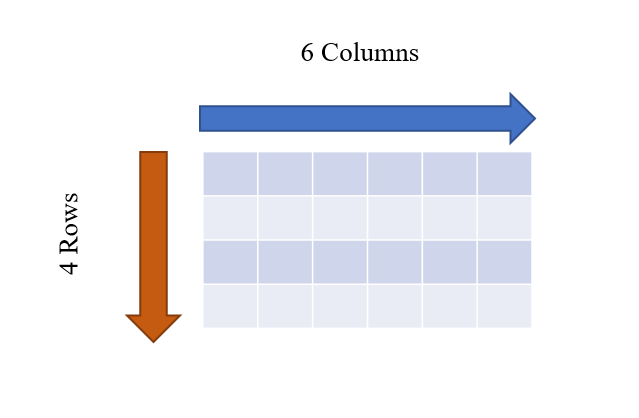
\includegraphics[width=0.8\textwidth]{./RowsAndColumns.png} % Adjust the Poidth as needed
	\caption{Confusingly, Columns are vertical, but you count them across a matrix; Rows are horizontal, but you count them vertically across a matrix}
\end{figure}

\begin{figure}[H]
    \centering
    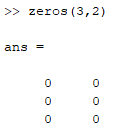
\includegraphics[width=0.3\textwidth]{./RowsColumnsCount.png} % Adjust the Poidth as needed
	\caption{\textbf{(Rows, Columns)}. Count Down, then across.}
\end{figure}

\subsection{Torch Templates}
\begin{figure}[H]
    \centering
    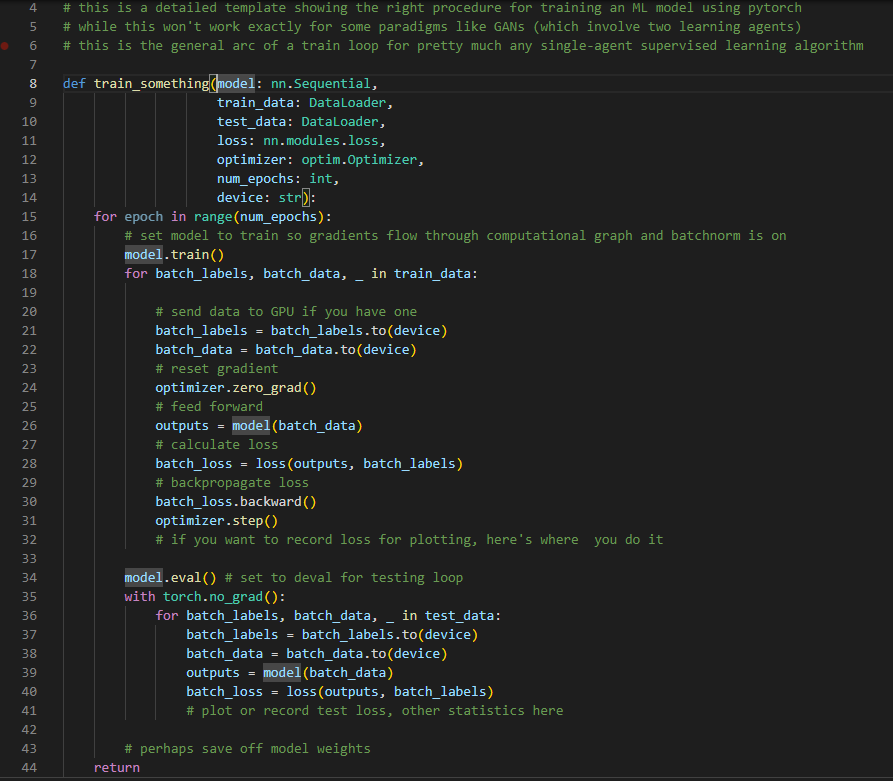
\includegraphics[width=1.0\textwidth]{./train_template_torch.png} % Adjust the Poidth as needed
	\caption{General Template for a train loop in a supervised single-agent learning algorithm.}
\end{figure}

\section{Review of Various Math Concepts}
\begin{itemize}
\item \textbf{Injection, Surjection, Bijection}: 
	\begin{figure}[H]
	    \centering
	    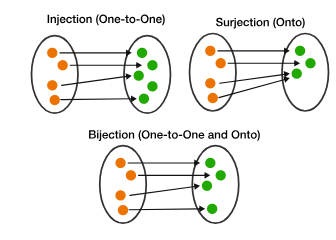
\includegraphics[width=0.6\textwidth]{./surjection.png} % Adjust the Poidth as needed
		\caption{\textbf{Injection}: Every element in input maps to a unique element in the  ouput. \\ \textbf{Surjection}: Every element in output is mapped to by at least one element in the input.\textbf{Bijection}: Every element in input maps to a unique element in the output, and every element in output has exactly one input mapping to it. Bijective functions are both injective and surjective.}
	\end{figure}
\item \textbf{Trace}: the trace of a square matrix is the sum of the diagonal elements of the matrix:\[\text{Tr}(A) = \sum_{i=1}^n A_{ii}\] Among other things, it is useful becuase the trace is used to calculate the derivative of the determinant of a matrix \(A\): \[\frac{d}{dt}\text{det}(A(t)) = \text{Tr}\left(\text{adj}(A(t)) \frac{dA(t)}{dt}\right)\] Where adj(\(A(t)\)) represents the adjugate of \(A\)
\item \textbf{Adjugate} The adjugate of a matrix is the transpose of its cofactor. For a \(2 \times 2\) matrix A: 

\[ A = 
\begin{pmatrix}
a & b \\
c & d
\end{pmatrix}
\]



\[ C =
\begin{pmatrix}
d & -c \\
-b & a
\end{pmatrix}
\]

\[ \text{Adj(A)} = C^T =
\begin{pmatrix}
d & -b \\
-c & a
\end{pmatrix}
\]

\item{Laplacian vs. Gradient}: For a twice-differentiable real-valued function \(f\), the Laplacian \(\Delta\) is the sum of the second partial derivatives with respect to each independent variable in the function. The gradient \(\nabla\) is the partial derivative of the equation with respect to each element of the vector: 
\[\nabla f = \left(\frac{\partial}{\partial x_1}, ... , \frac{\partial}{\partial x_n}\right)\]

\[\Delta f = \sum_{i=1}^n\frac{\partial^2f}{\partial x_i^2}\]
\end{itemize}
\section{Probing Classifiers (Advanced ML Concept)}
Probing classifiers are a methodology for interpreting deep neural network models for natural language processing, in particular LLMs. The basic idea is this: a simple classifier is trained to predict some challenging linguistic proprety from a model's internal representations, and the degree to which it learns to predict this proprety from the models internal representations offres us insight into the internal representations of the LLM itself. 
\subsection{Mathematical Formulation \& Justification}
Let some language model (I will say LLM from now on, because it is simpler to rely on that mental model and then attempt to generalize to other kinds of language models) be denoted like this:
\[f: x \rightarrow \hat{y}\]
Where LLM \(f\) is a function that maps input \(x\) to output \(y\). This is the original model. It is trained on some annotated dataset
\[\mathcal{D}_O = (x^{(i)}, y^{(i)})\]
Its performance is evaluated by some measure which we will denote as 
\[\mathcal{L}(f,\mathcal{D}_O )\]
The function \(f\) is typically a deep neural network that generates intermediate representations of x, for example, \( f_l(x) \) may denote the representation of x at layer l of f. A probing classifier \(z\) may map the immediate representation  \( f_l(x) \) to some property \(\hat{z}\), which is of linguistic interest:

\[g:f_l(x)\rightarrow \hat{z}\]
As a concrete example, f might be a sentiment analysis model, mapping a text x to a sentiment label y, while g might be a classifier mapping intermediate representations \( f_l(x) \) to part-of-speech tags z. The classifier \(g\) is then trained and evaluated on some other dataset
\[\mathcal{D}_P = (x^{(i)}, y^{(i)})\]
And some performance measure
\[\mathcal{L}(g,f,\mathcal{D}_O,\mathcal{D}_P )\]

\textbf{Important}: From an information theoretic perspective, the classifier \(g\) can be seen as estimating the mutual information \(I\) between the intermediate representations \(f_l(x)\) and the linguistic property \(z\): 
\[I(z, f_l(x)) = \mathbb{E}_{p(z,f_l(x))}\left[\log \frac{p(z, f_l(x))}{p(z)p(f_l(x))}\right]\]

\textbf{Why?}: If there having access to the residual stream \(f_l(x)\) does not improve the ability of the probing classifier to predict \(z\) at all, then \(p(z, f_l(x)) = p(z)p(f_l(x))\), which is the definition of statistical independence, and they have 0 mutual information. If on the other hand, the classifier is better at predicting \(z\) given access to the residual stream \(f_l(x)\), then  \(p(z, f_l(x)) > p(z)p(f_l(x))\) and we have positive statistical dependence and nonzero mutual information.

Where statistical independence is characterized  by this value being 0 and perfect statistical dependence being characterized as infinite (unreachable).

\section{Common ML Data Structures}
\subsection {Torch Dataloader}
Each element in a dataloader has structure: 

\[\text{[labels, data, indices]}\]
batchorm1d expects (N,C,L) by default, where 'C' is the channel/feature dimension it normalizes over
\subsection {Batchnorm}
\begin{figure}[H]
    \centering
    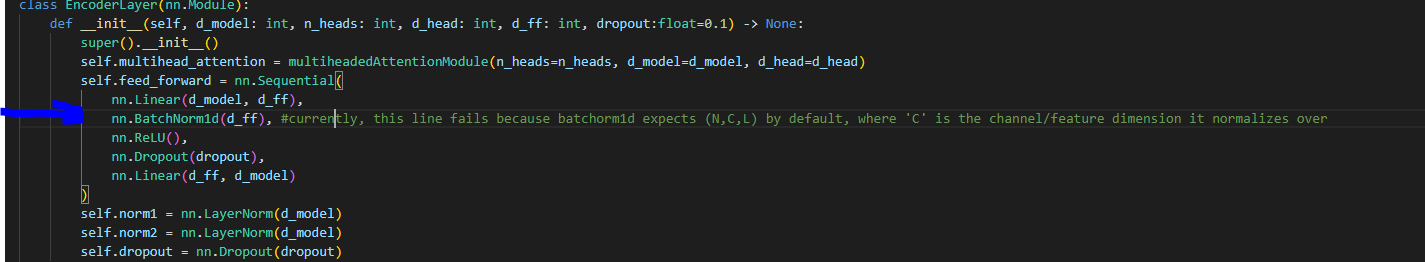
\includegraphics[width=1.0\textwidth]{./torch_batchnorm_error.png} % Adjust the Poidth as needed
	\caption{If input has shape [8,15,2048] and d\_ff is 2048, this will fail}
\end{figure}

\subsection{Einsum} Einsum is an extremely general way of performing tensor and ndarray operations. Can be used as a replacement for pretty much any tensor operation you can imagine and can combine multiple in a single einsum call.
\begin{figure}[H]
    \centering
    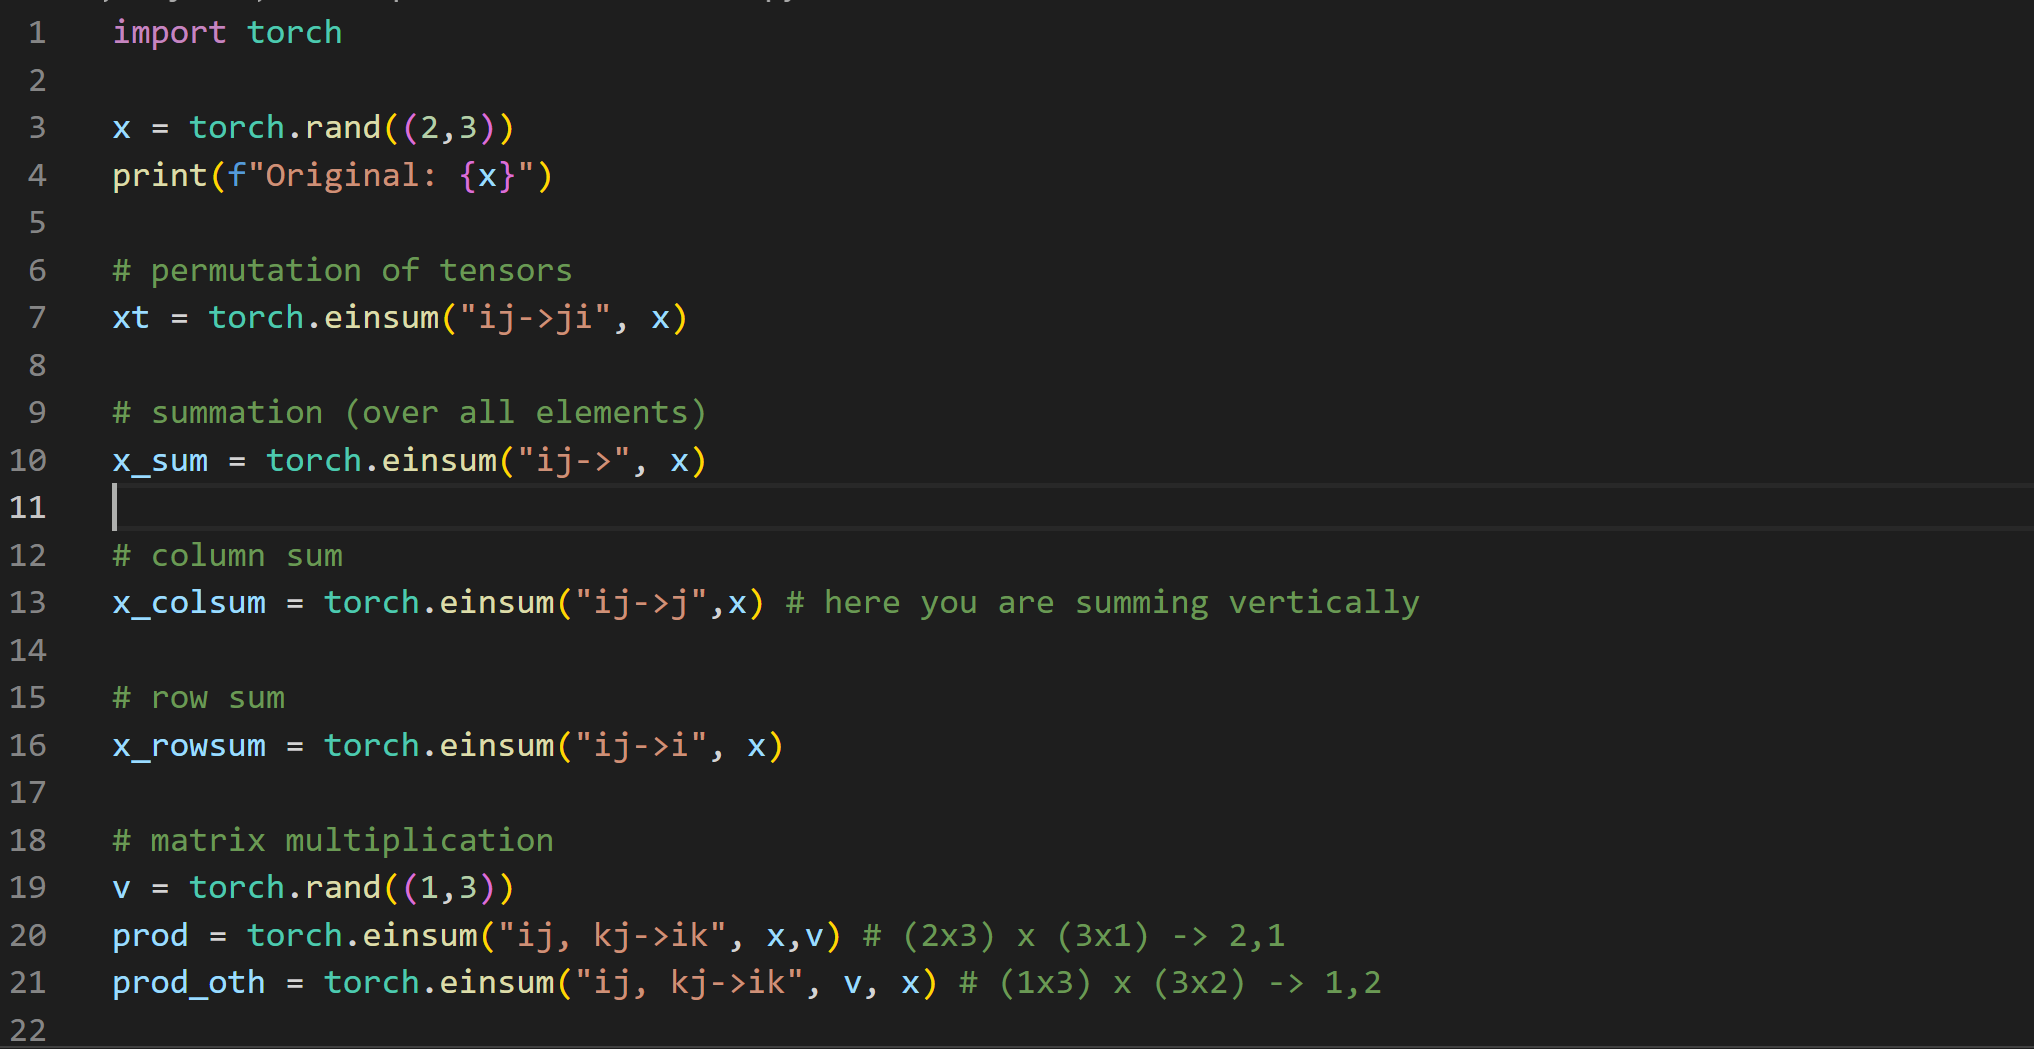
\includegraphics[width=1.0\textwidth]{./einsum_1.png} % Adjust the Poidth as needed
\end{figure}
\begin{figure}[H]
    \centering
    \includegraphics[width=1.0\textwidth]{./einsum_2.png} % Adjust the Poidth as needed
\end{figure}
\begin{figure}[H]
    \centering
    \includegraphics[width=1.0\textwidth]{./einsum_3.png} % Adjust the Poidth as needed
\end{figure}
\subsection{Numpy ufuncs}

Numpy is a python package designed to efficiently perfrom high-level mathematical functions on multidimensional arrays. \\


Ufuncs (universal functions) are functions that operate on ndarrays in an element-by-element fashion. Essentially, a ufunc is a vectorized wrapper for a function that takes a fixed number of specific inputs and produces a fixed number of specific outputs. For example, in the image below, add and multiply are both ufuncs. All ufuncs have a set of functionsthat operate on them including accumulate, reduce, etc. 
\begin{figure}[H]
    \centering
    \includegraphics[width=1.0\textwidth]{./ufunc.png} % Adjust the Poidth as needed
\end{figure}
Each on of these operators, wihch can be applied to any ufunc, has a serialized equivalent (like the one below for accumulate)

\begin{figure}[H]df
    \centering
    \includegraphics[width=1.0\textwidth]{./ufunc_eq.png} % Adjust the Poidth as needed
\end{figure}
\subsubsection{Time Complexity Analysis of Numpy Ufuncs}
For small array size, NumPy's additional optimizations and parallelization overhead outweigh the benefits of using its highly optimized C-backed functions. For larger arrays, NumPy outperforms my Python-based function due to its efficient use of vectorized operations and parallel computation.

\begin{figure}[H]
    \centering
    \includegraphics[width=1.0\textwidth]{./ufunc_analysis_code.png} % Adjust the Poidth as needed
\end{figure}

\begin{figure}[H]
    \centering
    \includegraphics[width=1.0\textwidth]{./ufunc_analysis_plot.png} % Adjust the Poidth as needed
	\caption{For small arrays, my serialized code is slightly faster. For larger arrays, Numpy's is much faster}
\end{figure}

\section {Definitions \& Tips}
\begin{itemize}
\item \textbf{One Shot Learning}: Learning paradigm in which we may only observe a single example of each possible class before having to make predictions about a test instance 
\item Batch size should be the first dimension of a tensor! \[Tensor = \{batchSize, inputs, outputs, channels\}\]
\item \textbf{Sufficient Statistic} In Detection \& Estimation Theory, a sufficient statistic for a parameter (or a set of parameters) of a statistical model is a function of the data if it provides as much information about the data as the parameter itself. That means a statistic \(T(X)\) is sufficient for some parameter \(\theta\) if the mutual information between  \(\theta\) and \(X\) is equal to the mutual information between  \(\theta\) and \(T(X)\):

\(I(\theta; T(X)) = I(\theta; X)\)

For example, a statistic \(T(X)\) is a sufficient statistic for some parameter \(\theta\) if the conditional probability of our observations \(X\)  given the statistic \(T(X)\) does not depend on \(\theta\): 
\[P(X=x | T(X)=t, \theta) = P(X=x|T(X)=t)\]
In other words, once \(T(X)\) is known, \(\theta\) provides no additional information abotu the dataset. \(T(X)\) is a sufficient statistic for \(\theta\) if and only if it obeys the Neyman-Fisher Factorization Theorem: 
\[f(x|\theta) = h(x)g(T(X)|\theta)\]
That is, \(T(X)\) is a sufficient statistic for \(\theta\) if and only if the conditional probability of observing x given our parameter \(f(x|\theta)\) can be decomposed into two functions: \(h(x)\): a function that does not depend on \(\theta\) at all; and \(g(T(x)|\theta)\): a functoin that depends on the data only through our statistic \(T(X)\). Sufficient statistics are important because they allow us to reduce the dimensionality of our estimation theory problem from \(n\) dimensions to 1 dimension without discarding any information. For example, if \(T(x) = \sum_{i=1}^n x_i\) is a sufficient statistic for some function, then we can make decisions based on the threshold of this single, one-dimensional value rather than having to try and make an n-dimensional decision threshold somehow. 

\item \textbf{Collinearity} Collinearity refers to a situation in statistics when two or more predictor variables in a multiple regresssion model are highly correlated. when variables are colinear, they provide redundant information about the dependent variable. PCA can eliminate collinearity concerns by projecting data into new feature space, but at the cost of creating less explainable features.
\item \textbf{Soft Classification}: refers to the process of assigning probabilities to each class rather than making a single, definitive class assignment.
\item \textbf{Stemming}: Stemming is a heuristic process from Natural Language Processing in which a word is reduced to its base or root form (the stem) by removing prefixes and suffixes. This is used to simplify the learning process by reducing the number of tokens, allowing the model to focus on the core meaning of the words rather than their different conjugations and forms. For example, "running", "runs", and "runner" might all be reduced to the stem "run". But it is a flawed process, because "better" likely will be reduced to "bet" and "university" and "universal" might be reduced to "univers".
\item \textbf{Lemmatization}: Lemmatization is a more advanced form of stemming that reduces a word to its lemma, or the base form that corresponds to a meaningful word in the language. Lemmatization uses morphological analysis to ensure that the root form is semantically valid. This usually means looking up the word in a dictionary and finding its canonical form (so now better becomes good rather than bet)

\item \textbf{YOLO}: YOLO Models (You Only Look Once) are a family of object detection and classification models which perform detection and classification in one forward pass, outputting both bounding boxes and class probabilities, rather than relying on Region Proposal Networks to perform detection, with an additional classification network layered on top. They are intended for real-time object detection and classification. 

\item \textbf{One-Shot Learning}: One-Shot Learning is a technique which aims to perform classification on classes with few (or even just 1) training sample per class. \\ 
\textbf{Procedure}: First, you train a classifier on a large, open source dataset like imagenet containing many different images and classes. You train it via contrastive loss or triplet loss, with the intent of learning a feature representation which groups images in the same class closely together and images in different classes farther apart. Then, you supply it with support images (to be used at inference time), one from each class you wish to peform inference on. Then you perform inference on the new class set with no additional training.\\
\textbf{Note}: You are training on one class set with many samples (e.g. dog, cat, giraffe) and then performing inference on images belonging to classes your model has never seen (e.g: palm tree, pine tree, cherry tree).
\item \textbf{Few-Shot Learning}: Few shot learning is the same premise as one shot learning, except now instead of just one support image per target class you have several (usually 2-10). The training procedure is exactly the same: you still train a model to learn feature representations on a base dataset, then use those (along with support images) to generalize to a new inference class set. The difference is taht in few shot learning there are some ways to leverage having multiple images to enhance the generalizeability of your feature representations. These include:
\begin{enumerate}
\item Averaging Embeddings / Prototypical Networks: For each target class, generate embeddings of the support examples and average them to produce a prototype for the class. then use this embedding as anchor at inference.
\item Nearest Neighbors: compare the query image to each individual support example and classify the query based on the nearest neigbhor.
\end{enumerate}
\end{itemize}

\section{Software Engineering Patterns}

\subsection{Data Structures}
\subsubsection{Linked Lists}
Linked Lists are a common data structure consisting of a sequence of elements whose order is not given by their placement in memory; rather, each element points to the next:
\begin{figure}[H]
    \centering
    \includegraphics[width=0.8\textwidth]{./linked_list.png} % Adjust the width as needed
    \caption{The basic linked list architecture}
\end{figure}
\textbf{Problem Solving Tips}
\begin{enumerate}
\item \textbf{Reversing Linked List}: When reversing linked lists, you should always physically write out your lines of code on a sheet of paper or (preferably) a whiteboard; it's far easier to keep track of exactly what the pointers are doing this way.
\begin{figure}[H]
    \centering
    \includegraphics[width=0.8\textwidth]{./reverse_linked_list.png} % Adjust the width as needed
    \caption{Basic function to reverse a linked list}
\end{figure}
\item \textbf{Tortoise and Hare}: Use a slow pointer that iterates 1 node at a time and a fast pointer that iterates two nodes at a time (e.g problem: finding midpoint of linked list).
\item \textbf{Dummy Nodes}: Initializing a dummy listnode such that dummy.next = head is useful for handling edge cases involving the head node.
\end{enumerate}
\subsubsection{Doubly Linked Lists}
A linked list but each node keeps track of  both the previous and next node:
\begin{figure}[H]
    \centering
    \includegraphics[width=0.7\textwidth]{./DLL.png} % Adjust the width as needed
\end{figure}
\subsection{Algorithms}
\subsubsection{Dynamic Programming}
Dynamic Programming is a programming technique where you simplify complicated problems by breaking them down into smaller subproblems. Typically, it includes both recursion and memoization.\\


\textbf{Memoization} Memoization is a technique used to optimize recursive algorithms by storing the results of expensive function calls and reusing them when the same inputs occur again. It involves creating a lookup table (often implemented using arrays or hash maps) that maps from the function's input parameters to the computed results.\\

So dynamic programming \(=\) Recursion + Memoization. \\
Fundamentally, there are two types of dynammic programming problems:\\
\begin{enumerate}
\item \textbf{Optimization Problems}: Find whether a given solution is possible, find the best solution possible
\item \textbf{Counting Problems}: Find the number of ways something can be done
\end{enumerate}



\subsubsection{Sliding Window Techniques}
Sliding windows problems are a dynamic programming technique used for finding subarrays in an array that satisfy given conditions. \\

Oftentimes (like dynammic programming problems), they can be used to solve problems in \(O(n)\) time and \(O(1)\) space that would require exponential time under a naive approach. \\

\textbf{Examples}
\begin{enumerate}
\item \textbf{Longest Unique Substring} Find the longest substring without repeating characters

\begin{figure}[H]
    \centering
    \includegraphics[width=0.8\textwidth]{./slidingwindow.png} % Adjust the width as needed
\end{figure}
\item \textbf{Minimium Size of Subarray Sum}: Given an array of positive interger
\end{enumerate}

\textbf{When you can use}
\textbf{Tips}
\begin{enumerate}
\item \textbf{Nested While loops are your friend}: Usually a bad idea. But in this case they work. Inner while loop controls when to shrink the array once the condition is met. Outer while loop controls growing the array. 
\item \textbf{Remember to make sure the subarray can grow/shrink properly throughout the entire array (especially at the end)}
\item \textbf{Use Two pointers}: You'll almost always want to use two pointers to keep track of your subarray. \textbf{These pointers can do more than you think}. If you find yourself instantiating a list to keep track of the subarray, the odds are quite good this is unecessary (that said, it's always good to implement a naive solution first and then optimize afterwards).
\item \textbf{Don't use recursion}: If you are corrent that a problem can be solved with a sliding window, you NEVER should use recursion. You'll likely get out of memory errors and in any case it will complicate your solution unecessarily. 
item \textbf{If dealing with ints and sums, you need positive intergers}: Kadane's algorithm works with arrays that contain 0's or negatives, but if you don't know that, solving this problem without Kadane's algorithm is extremely complicated. \textbf{Pro Tip}: if you are confronted with an array that has negatives, find the largest negative and add the absolute value of that negative plus 1 to the array so you don't need to deal with negatives. Not a good solution for production algorithms, but for coding interviews it will do the trick. 
\end{enumerate}

\section{Heaps}
Heaps are a fundamental data structure. They are a specialized kind of binary search tree that satisfy the \textbf{Heap Property}:
\begin{itemize}
\item \textbf{Max Heap Property} The key of each node is greater than or equal to the keys of its children
\item \textbf{Min Heap Property} The key of each node is less than or equal to the keys of its children
\end{itemize}
Beyond this property, heaps (max and min heaps) satisfy the following additional properties:
\begin{itemize}
\item \textbf{Complete Binary Tree}: Heaps are complete binary trees, meaning all levels are fully filled except possibly the last level, which is filled left to right
\item \textbf{O(1) Access}: Root element of a max heap is the largest, and the min-heap is the smallest, so there's O(1) lookup time for max/min
\item \textbf{O(log(n)) Insertion and Deletion}: Insertion and deletion involve maintaining the heap property and both have a time complexity of O(log n)
\end{itemize}

Heaps are represented as a list where the left child of node \(i\) is at \(2i+1\) and the right child of node \(i\) is at \(2i+2\).

\begin{figure}[H]
    \centering
    \includegraphics[width=0.8\textwidth]{./Heap-as-array.png} % Adjust the width as needed
\end{figure}

Here's how to code each key function in a max heap:
\begin{itemize}
\item \textbf{Insert}: Add new element to last index of array. Bubble up with heapify
\item \textbf{Remove}: Swap first and last element of array. Pop last element. Bubble Down with heapify
\item \textbf{Bubble Up Heapify}: For insertions. Start at -1st index. While \((i-1)>i//2\), swap indices (use \((i-1)>i//2\)) whenever you're in a 0-indexed language). When this ends,  you'll have all elements in array satisfying heap property. O(log n) time complexity.
\item \textbf{Bubble Down Heapify}: For deletions. Start at 0th index. If \(i\) has no children, return.If \(i\) is larger than its children, return. If \(i\) has one child, swap i and that child if the child is larger than the parent. If it has two children, swap the parent and the larger child. This will also preserve heap property once function terminates. Also O(log n) time complexity
\end{itemize}
\begin{figure}[H]
    \centering
    \includegraphics[width=0.8\textwidth]{./heapify.png} % Adjust the width as needed
\end{figure}
\section{LRU Caches}
A LRU (Least Recently Used) Cache is a data structure that combines a DLL (Doubly Linked List) and a hashmap to provide a cache that efficiently manages memory by retaining the \(n\) most recently used entries, while allowing for \(O(1)\) lookup, insert, and delete operations. Here are the implementation details in the form of four key operations a LRU Cache Must Perform:
\begin{itemize}
\item{Get(key)}: For returning value in \(\{\text{key, value}\}\) pair. Algorithm: If key in self.cache, get node at self.cache[key]. Remove it from the DLL and add it back as the 0th element. return node.val 
\item{Put(key, value)}: For inserting a new \(\{\text{key, value}\}\) pair into the LRU Cache. Algorithm: If key in self.cache, get node at self.cache[key]. Remove it from the DLL and add it back as the 0th element. Otherwise, and if we're at capacity, get the least recently used element at self.tail.prev, delete if from the cache (del self.cache[lru\_node.key]). then add the new element Node(key,value) into both the cache and the doubly linked list.
\item{Add and Remove}: both of these are just adding / removing an element from a doubly linked list. O(1) time both of them if implemented properly.
\end{itemize}
\begin{figure}[H]
    \centering
    \includegraphics[width=1.0\textwidth]{./LRU\_cache.png} % Adjust the width as needed
	\caption{Python Implementation of a LRU Cache. Node is a standard doubly linked list as defined above in DLL Section.}
\end{figure}
\section{Binary Search}
Binary Search is a \texttt{O(log n)} algorithm for performing search over a sorted list. In Binary Search, we progressively reduce the search space by \(\frac{1}{2}\) each time we search, ensuring a logarithmic number of iterations. \\

Below is the most elementary possible function for binary search. Note that there is a way to make this work without any return statement in the while loop that is slightly more elegant, but I don't understand that way super well because it involves a sophsticated understanding of the edge cases, which I don't really have:
\begin{figure}[H]
    \centering
    \includegraphics[width=1.0\textwidth]{./needleHaystack.png} % Adjust the width as needed
	\caption{Python Implementation of a Binary Search Algorithm.}
\end{figure}
\section{Binary Trees}
Binary Trees are a basic data structure where each node has a left child and a right child. Trees can be represented explicitly using a class definition:
\begin{figure}[H]
    \centering
    \includegraphics[width=1.0\textwidth]{./treedef.png} % Adjust the width as needed
	\caption{Python Implementation of Tree.}
\end{figure}
or implicitly in the form of a list (this is what heaps are). \textbf{Binary Search Trees} are trees that meet specific conditions which guarantee efficient lookup, insert, and delete operations: 
\begin{table}[H]
\centering
\resizebox{0.9\textwidth}{!}{%
\begin{tabular}{|c|c|c|}
\hline
\textbf{Feature}        & \textbf{Binary Tree}          & \textbf{BST}                  \\ \hline
\textbf{Node Order}     & No specific order.            & Left \(<\) Root \(<\) Right.          \\ \hline
\textbf{Search Time}    & \(O(n)\)                      & \(O(\log n)\) (balanced).     \\ \hline
\textbf{Insert Time}    & \(O(1)\) (arbitrary).         & \(O(\log n)\) (balanced).     \\ \hline
\textbf{Delete Time}    & \(O(n)\)                      & \(O(\log n)\) (balanced).     \\ \hline
\textbf{In-order}       & No specific order.            & Produces sorted output.       \\ \hline
\textbf{Duplicates}     & Allowed.                      & Typically not allowed.        \\ \hline
\end{tabular}%
}
\caption{Binary Tree vs. BST}
\end{table}

Here is C++ code for the in-order traversal of a binary tree:
\begin{figure}[H]
    \centering
    \includegraphics[width=1.0\textwidth]{./inorder.png} % Adjust the width as needed
	\caption{Python Implementation of Tree.}
\end{figure}

Note that post-order is literally the exact same algorithm except you add (left nodes, right nodes, root node). So the only thing you change is the position you add the root node in. EVERYTHING else is the same.
\begin{figure}[H]
    \centering
    \includegraphics[width=1.0\textwidth]{./postorder.png} % Adjust the width as needed
	\caption{Inorder Traversal of a Binary Tree in C++.}
\end{figure}

And same with preorder traversal. the only thing that is different is that you go (root node, left nodes, right nodes):
\begin{figure}[H]
    \centering
    \includegraphics[width=1.0\textwidth]{./preorder.png} % Adjust the width as needed
	\caption{Postorder Traversal of a Binary Tree in C++.}
\end{figure}
And here are the examples of what the in-order, pre-order, and post-order traversal of the following binary tree are:

\begin{figure}[H]
    \centering
    \includegraphics[width=1.0\textwidth]{./tree\_ex.png} % Adjust the width as needed
	\caption{Preorder Traversal of a Binary Tree in C++.}
\end{figure}
\begin{table}[H]
\centering
\begin{tabular}{|c|l|}
\hline
\textbf{Traversal Type} & \textbf{Traversal Order}                       \\ \hline
In-order                & [4, 2, 6, 5, 7, 1, 3, 9, 8]                   \\ \hline
Pre-order               & [1, 2, 4, 5, 6, 7, 3, 8, 9]                   \\ \hline
Post-order              & [4, 6, 7, 5, 2, 9, 8, 3, 1]                   \\ \hline
\end{tabular}
\caption{Traversals of the Binary Tree.}
\end{table}
\section{Kadane's Algorith \& Maximum Subarray Problem}
Kadane's algorithm is an algorithm for solving the maximum subarray problem: Given an array of \(n\) integers, find the sum of the maximum subarray:

\[m = [1, 2, -4, 3, 6, -2, 1, 6, -4]\]

This is the algorithm: 

\begin{figure}[H]
    \centering
    \includegraphics[width=1.0\textwidth]{./kadane.png} % Adjust the width as needed
\end{figure}

To find the maximum circular subarray, we simply take the maximum subarray using Kadane's algorithm, and the minimum subarray using kadane's algorithm. then we subtract the maximum and the minimum. Why does this work? One of two things must be true for the maximum circular subarray:
\begin{enumerate}
\item The max subarray does not rely on the circular property (in this case we just need the maximum subarray as described above)
\item The max subarray \emph{does} rely on the circular property. In this case the max sum is equal to tghe sum of the total array minus some minimal subarray that is 'taken out' in the middle. We can find the min subarray to remove using kadane's algorithm with the signs reversed.
\end{enumerate}

\section{Combinatorics}
\subsection{Combinations}
The number of ways to choose \(k\) items from a set of \(n\) items without regard to the order of selection:
\[
\binom{n}{k} = \frac{n!}{k!(n-k)!}
\]

\subsection{Permutations}
The number of ways to arrange \(k\) items from a set of \(n\) items where the order does matter:
\[
P(n,k) = \frac{n!}{(n-k)!}
\]

\textbf{Why is the number of permutations greater than or equal to the number of combinations?} Because permutations to combinations is a many-to-one surjection. Specifically, \(\binom{n}{k}\) and \(P(n,k)\) differ by a factor of \(k!\) because there are exactly \(k!\) ways to permute any given arrangement of \(k\) items.

How does adding an \((n+1)^{\text{th}}\) element impact \(\binom{n}{k}\)?

\[
\binom{n}{k} = \frac{n!}{k!(n-k)!}
\]

So adding an \((n+1)^{\text{th}}\) element:
\[
\binom{n+1}{k} = \frac{(n+1)!}{k!(n+1-k)!}
\]

This expands to:
\[
\frac{(n+1)\cdot n!}{k! \cdot (n-k)! \cdot (n+1-k)}
\]

This is equal to:
\[
\frac{n!}{k!(n-k)!} \cdot \frac{(n+1)}{(n+1-k)}
\]

So this means \(\binom{n+1}{k}\) differs from \(\binom{n}{k}\) by a factor of \(\frac{n+1}{n+1-k}\).

Example: \(\binom{5}{3} = 10\).  
\(\binom{6}{3} = \binom{5}{3} \cdot \frac{5+1}{5+1-3} = \binom{5}{3} \cdot 2 = 20\).

\subsection{Catalan Numbers}
Catalan Numbers are a sequence of natural numbers that occur in many different kinds of counting problems. The formula for the \(n^{th}\) Catalan number is given by

\[
C_n = \frac{1}{n+1} \binom{2n}{n} = \frac{1}{n+1} \frac{(2n)!}{n!(2n - n)!}
\]

Simplifying, the \(n^{th}\) Catalan number is

\[
C_n = \frac{(2n)!}{(n+1)!n!}
\]
so the first Catalan numbers for \(n=0, 1, 2, 3, \ldots\) are
\[1, 1, 2, 5, 14, 42, 132, 429, 1430, 4862, 16796, 58786, \ldots\]

\subsubsection{Problems}
\begin{enumerate}
\item \textbf{Dyck Words}: 
    \(C_n\) is the number of Dyck words of length \(2n\). A Dyck word is a string consisting of \(n\) \(X\)'s and \(n\) \(Y\)'s such that no initial segment of the string has more \(Y\)'s than \(X\)'s. For example, the following are the Dyck words up to length 6:
    \[
    XY,
    \]
    \[
    XXYY, \quad XYXY,
    \]
    \[
    XXXYYY, \quad XXYXYY, \quad XYXXYY, \quad XYXYXY, \quad XXYYXY.
    \]

    Re-interpreting the symbol \(X\) as an open parenthesis and \(Y\) as a close parenthesis, \(C_n\) counts the number of expressions containing \(n\) pairs of parentheses which are correctly matched:
    \[
    (()()), \quad (())(), \quad ()(()), \quad ()()(), \quad ((()))
    \]

\item \textbf{Number of Structurally Unique Binary Search Trees}: \(C_n\) is the number of structurally unique BSTs with exactly \(n\) internal nodes, or equivalently, with \(n+1\) leaves. 
\end{enumerate}

\subsection{Stars and Bars (or balls and bins) problem}
How many different ways can you distribute \(n\) identical balls into \(k\) identical bins? Answer: 
\[\binom{n+k-1}{k-1}\]
Proof by induction:\\

Base Case: Distribute \(n=1\) balls across \(k\) bins. The answer to  this should be k.\\

\[\binom{1+k-1}{k-1} = \binom{k}{k-1}\]
\[\binom{k}{k-1} = \frac{k!}{(k-1)! \cdot (k - k + 1)!} = \frac{k!}{(k-1)! \cdot (1)!} = \frac{k!}{(k-1)!} = k \]
Inductive Case: Assume the inductive hypothesis is true for \(n\) balls distributed into \(k\) bins:
\[\binom{n+k-1}{k-1}\]
Prove it is true for \(n+1\) balls distributed into \(k\) bins. Proof:\\

Imagine we put \(i\) balls in box \#1. The remaining \((n+1)-i\) balls must go into the other \(k-1\) boxes. Under the inductive hypothesis, the number of ways to put \(m = (n+1)-i\) balls into \(k-1\) boxes is:
\[\binom{m+(k-1) - 1}{(k-1)-1} = \binom{(n+1)-i+k - 2}{k-2} =  \binom{n+k - i - 1}{k-2}\]
Because the choice of the number \(i\) is \textbf{mutually exclusive} (non-overlapping) and \textbf{collectivel exhaustive} (cover every possibility), the sum across all \(i\) of the number of ways to distribute the remaining \(n-i\) balls gives us the number of ways to distribute \(n+1\) balls:
\[\binom{n+k}{k-1}  = \sum_{i=0}^n \binom{n+k - i - 1}{k-2}\]
It can be shown that the identity above is true using the hockey stick identity (I don't really understand how that works though and I think this is enough detail for our purposes). so we've proven that the answer to the \(n\) balls and \(k\) bins problem is:
\[\binom{n+k-1}{k-1}\]
\subsection{Knapsack Problems}
Knapsack problems are a class of combinatoric optimization problem. Imagine you have a knapsack with a maximal weight capacity of \(\mathcal{C}\), a list of \(n\) items each with weight and value \((v_i, w_i)\), and your goal is to get the highest total value of items into the knapsack without exceeding its weight capacity. \\

The key to solving knapsack problems is finding the DP State Transition Relation, which governs the rule for updating the \texttt{DP[j]} based on \texttt{DP[0:j]}. For the \emph{Unbounded Knapsack Problem}, in which any item can be included arbitrarily many times, the relation is this:
\[DP[j] = \max \left(DP[j], DP[j-w[i]]+v[i]\right)\]

Where \((v_i, w_i)\) gives the weight and value of the \(i^{th}\) item we could include. Note that we have to iterate over each of the \(i\) items each time we fill in a new index \(j\) in our DP Table. Also note that with the unbounded problem this is a 1D DP Table. The bounded problem has a 2D DP Table:
\[
DP[j][i] = 
\begin{cases} 
\max\left(DP[j][i-1], DP[j - w[i]][i-1] + v[i]\right) & \text{if } w[i-1] \leq j, \\
DP[j][i-1] & \text{if } w[i-1] > j.
\end{cases}
\]

Here, \(DP[j][i]\) represents the maximum value achievable using the first \(i\) items (sequentially) and a knapsack capacity of \(j\). Note that with the bounded problem, this is a 2D DP Table because we track both the number of items considered (\(i\)) and the knapsack capacity (\(j\)). \\

The final solution for the bounded knapsack problem is found at:
\[
DP[n][\mathcal{C}]
\]
where \(n\) is the total number of items, and \(\mathcal{C}\) is the maximum capacity of the knapsack. It's worth noting that the dp table does not guarantee every entry is the global optimum, just that the final column for each capacity is an optimum. \\

\textbf{Question}: "I don't believe this works. show me it would work for both [7, 5, 3] and [7, 3, 5] with a capacity of 8. How will it avoid the local maximum." \\
\textbf{Answer}: I'm glad you asked. First, it will work for both of these because the dp table will correctly take \(\max\left(dp[8][1]=7, dp[8-5][2-1]+v[2]\right)\) where \(dp[3][1]\) will correctly give \(3\) and \(v[2]\) will be \(5\), so it will take \(\max(7,8)\) when we have items=\([(7,7),(3,3),(5,5)]\). And if we flip the 5 and the 3 then \(v[2]=3\) instead.
\section{Intro to Pandas}
Pandas is a data science package in python that is popular for machine learing and data science projects. it has lots of useful functions and in many ways is the pythonic answer to R. Here are some loose and disogranized notes with a few useful techniques for pandas:
\begin{enumerate}
\item \texttt{.apply()}: The  \texttt{.apply()} method will apply a function to each member of a pandas series (a column of a dataframe). It accepts a callable as its input and can handle built-in functions like len, anonymous functions, or custom function handles. Here's a quick chatGPT generated screenshot of an example with an anonymous function:
\begin{figure}[H]
    \centering
    \includegraphics[width=0.8\textwidth]{./apply.png} % Adjust the width as needed
\end{figure}
\end{enumerate}

\section{Glossary of C++ Terms}
Developing in C++ is a completely different experience from python. In my mind, it is the purest kind of SWE experience. In higher level languages you have so little control over the hardware it's easy to lose sight of the fact that you're really working intimately with a machine, and lower level languages like C and fortran are so enmeshed in the hardware that you lose sight of the higher level SWE things that matter in the real world. C++ is a happy medium, but it is harder to develop in than python. Here is a glossary of common terms and concepts and what they mean/do:\\
\begin{itemize}
\item \textbf{Namespace}: A namespace is a way to organize and group related code elements. It provides a \emph{named scope} for your variables, functions, and other identifiers. This means if you have, for examle, two different functions with the same name like this:
\begin{figure}[H]
    \centering
    \includegraphics[width=0.8\textwidth]{./namespace.png} % Adjust the width as needed
\end{figure}
If you imported both these in another file, there's ambiguity, and you don't know which \(\texttt{printMessage()}\) function will call:
\begin{figure}[H]
    \centering
    \includegraphics[width=0.8\textwidth]{./namespace\_prob.png} % Adjust the width as needed
\end{figure}
But if instead we encapsulate each of these functions inside its own namespace, we resolve the ambiguity
\begin{figure}[H]
    \centering
    \includegraphics[width=0.8\textwidth]{./namespace\_soln.png} % Adjust the width as needed
\end{figure}
\item \textbf{CMakeLists.txt}: CMakeLists.txt is a kind of configuration file used by CMake, a powerful build-system generator. It defines how your C++ file should be built: what source files should be compiles, what libraries it should link against, and what build options to use.
\item \textbf{Link Against}: What does it mean to "link against" something? If you "link against" a library when building your project, binary from that library is included in your project and can be directly called by methods in your project. 
\item \textbf{Allocating Memory}: Use Malloc/free together; use new/delete together. Malloc/free is c-style memory allocation where you're just given a pointer to an unstructured hunk of memory you can do whatever you want with; new gives you a hunk of memory that \texttt{new} then strucutres to the type that you want to populate it. In fact, new will also dynamically populate it. \texttt{Node* x = new Node(0,1);} will put 0 and 1 in the appropriate fields of \texttt{Node}. Actually, this isn't totally correct. What  actually does is 
\begin{enumerate}
\item create a strucutred block of memory 
\item Then the constructor \texttt{Node(0,1);} gets called. It populates that memory. This \texttt{new} doesn't explicitly do that part. 
\end{enumerate}
\item \textbf{Calloc vs. Malloc and Memset}: Calloc is similar to malloc but initializes all allocated memory to 0:
\[\texttt{int* dp = (int*)calloc(k, sizeof(int));}\]
Note that it only works for ints and because of that you don't have to do \texttt{k * sizeof(int)} as you would with malloc. Both return \texttt{void*} objects. you can do the same as above with the following two lines: 
\[\texttt{int* dp = (int*)malloc(k*sizeof(int));}\]
\[\texttt{memset(dp, 0, k*sizeof(int));}\]
Note that \texttt{Memset} sets all bytes in an already-allocated block to a specific value. 

\[\texttt{void* memset(void* ptr, int value, size\_t num);}\]

You can use it for other primitives such as \texttt{char} (but only primitives! trying to do \texttt{memset(str, 0, 5 * sizeof(std::string))} would result in undefined behavior):
\[
\begin{array}{l}
\texttt{// Example: Allocate memory and set everything to 'c'} \\
\texttt{char* buffer = (char*)malloc(10 * sizeof(char));} \\
\texttt{memset(buffer, 'c', 10 * sizeof(char));} \\
\texttt{// Now buffer contains: ['c', 'c', 'c', ..., 'c']}
\end{array}
\]
\end{itemize}
\end{document}
